% LaTeX Appendix - CFD Simulation Results
% Generated automatically from AppendixPlots directory
% Use with subfiles package: \subfile{path/to/this/file}

\appendix
\part{Appendices}

\chapter{CFD Simulation Results}
\label{chap:cfd_results}

% Increase TOC depth to show detailed navigation
\setcounter{tocdepth}{4}

This appendix presents the complete set of CFD simulation results organized by experiment type, Reynolds number, mesh resolution, and discretization scheme.

\section*{Channelflow Results}
\addcontentsline{toc}{section}{Channelflow Results}
\label{sec:channelflow_results}

\subsection*{Reynolds Number 10}
\addcontentsline{toc}{subsection}{Reynolds Number 10}
\label{subsec:channelflow_re10}

\subsubsection*{Medium Mesh}
\addcontentsline{toc}{subsubsection}{Medium Mesh}
\label{subsubsec:channelflow_re10_medium}

\paragraph*{Unstructured Mesh with TVD Scheme}
\addcontentsline{toc}{paragraph}{Unstructured Mesh with TVD Scheme}
\label{para:channelflow_re10_medium_unstructured_TVD}

\begin{figure}[H]
    \centering
    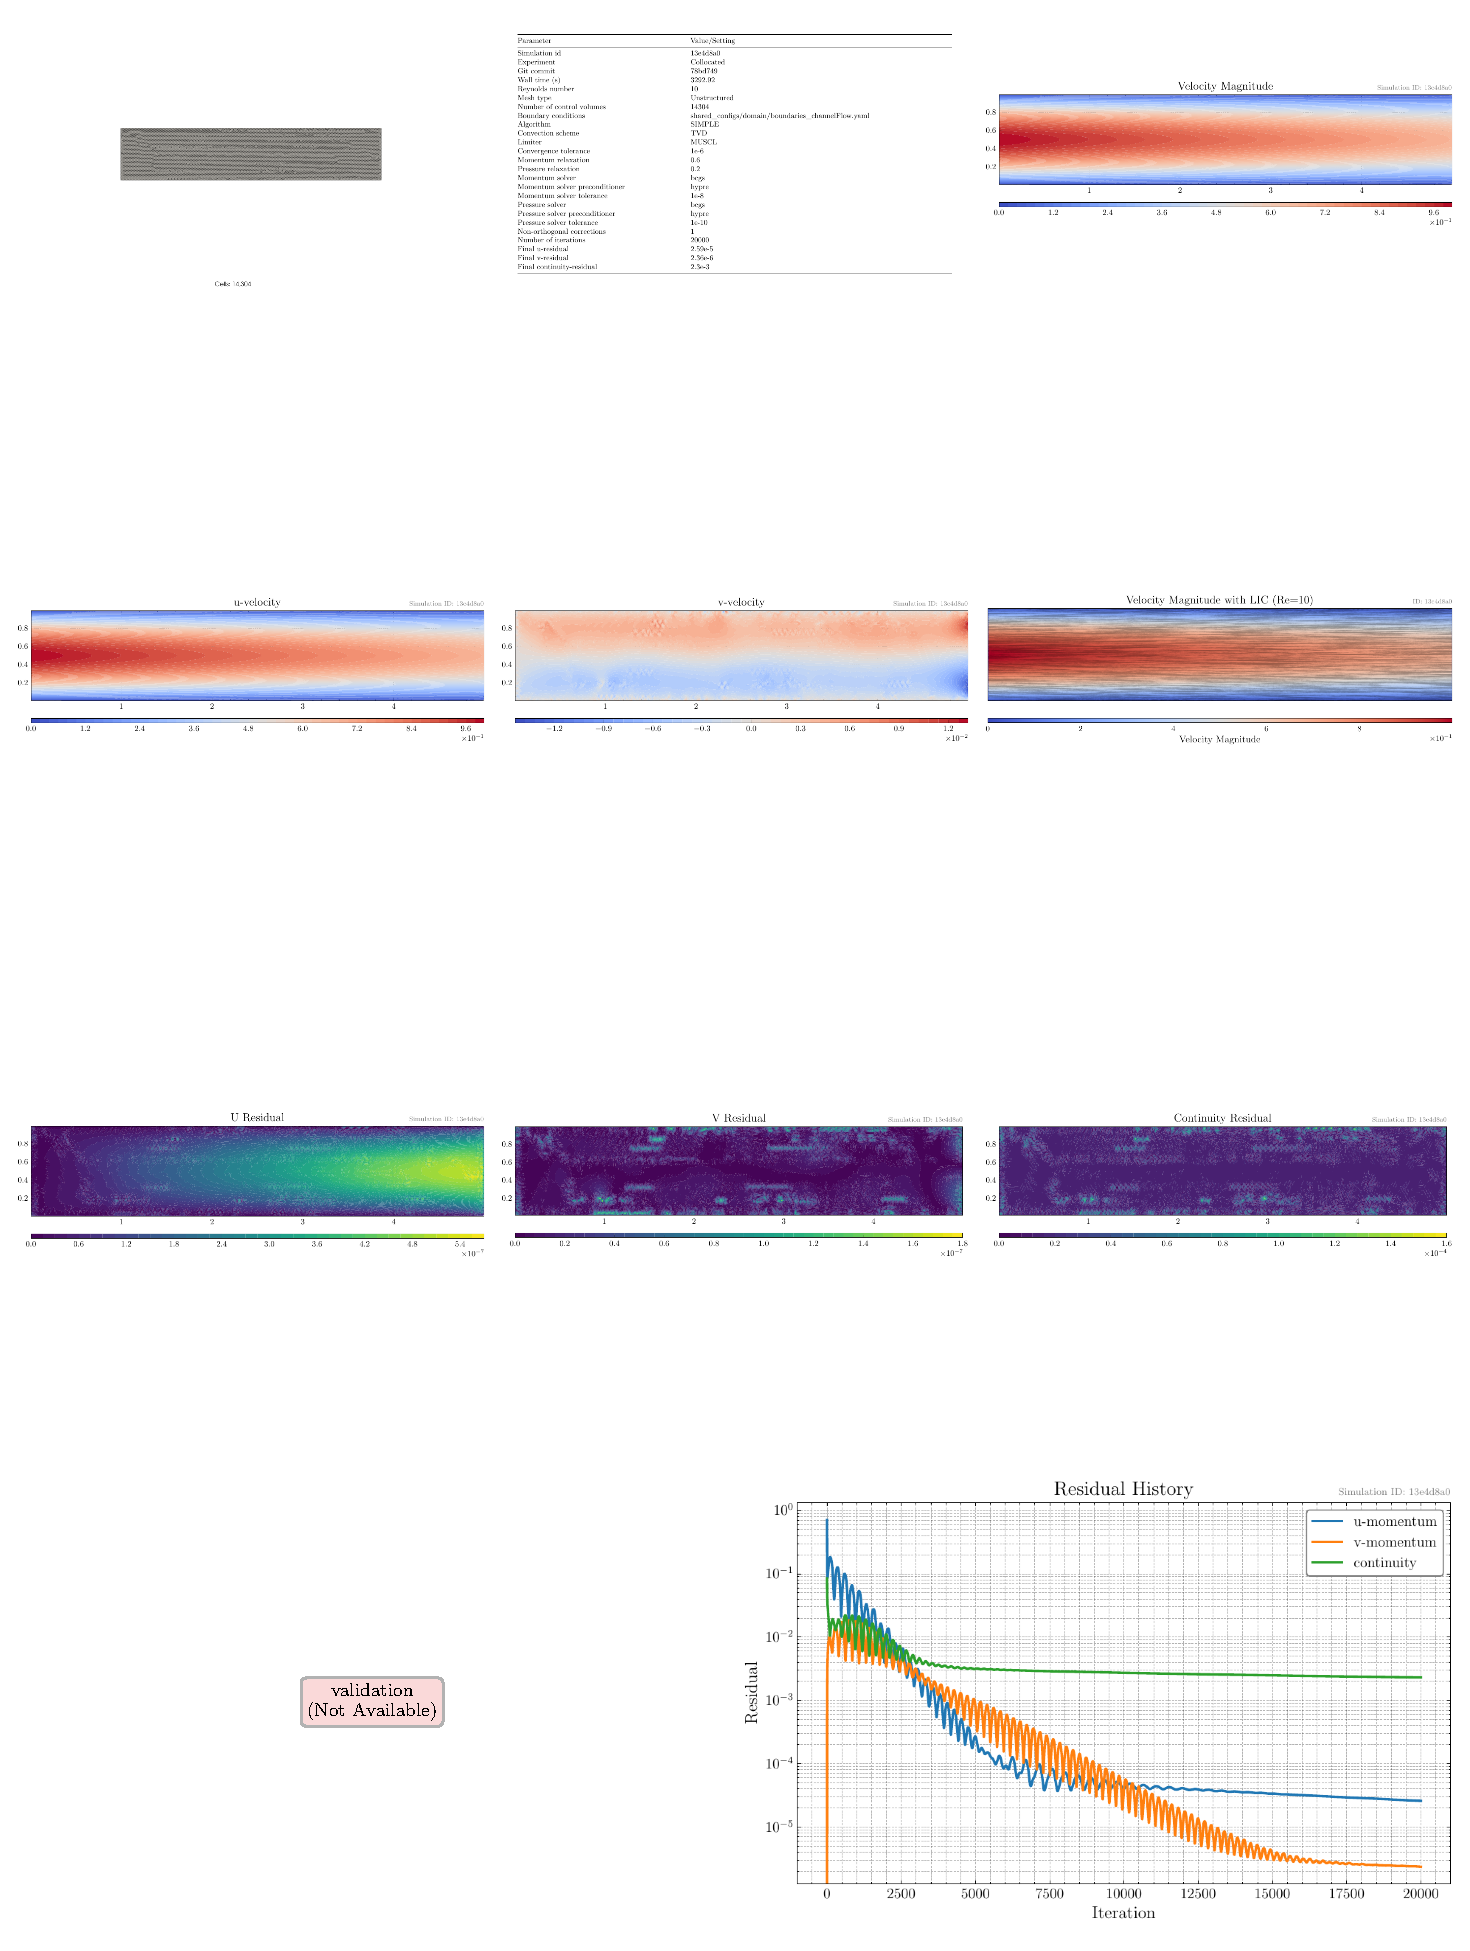
\includegraphics[width=0.85\linewidth]{AppendixPlots/channelFlow/Re_10/medium/channelFlow_Re10_unstructured_medium_TVD_13e4d8a0.pdf}
    \caption{Channelflow simulation at Re=10 using unstructured medium mesh with TVD discretization scheme (Simulation ID: 13e4d8a0)}
    \label{sim.cf.re10.unstruct.med.tvd}
\end{figure}

\clearpage

\section*{Cylinderflow Results}
\addcontentsline{toc}{section}{Cylinderflow Results}
\label{sec:cylinderflow_results}

\subsection*{Reynolds Number 3}
\addcontentsline{toc}{subsection}{Reynolds Number 3}
\label{subsec:cylinderflow_re3}

\subsubsection*{Medium Mesh}
\addcontentsline{toc}{subsubsection}{Medium Mesh}
\label{subsubsec:cylinderflow_re3_medium}

\paragraph*{Unstructured Mesh with TVD Scheme}
\addcontentsline{toc}{paragraph}{Unstructured Mesh with TVD Scheme}
\label{para:cylinderflow_re3_medium_unstructured_TVD}

\begin{figure}[H]
    \centering
    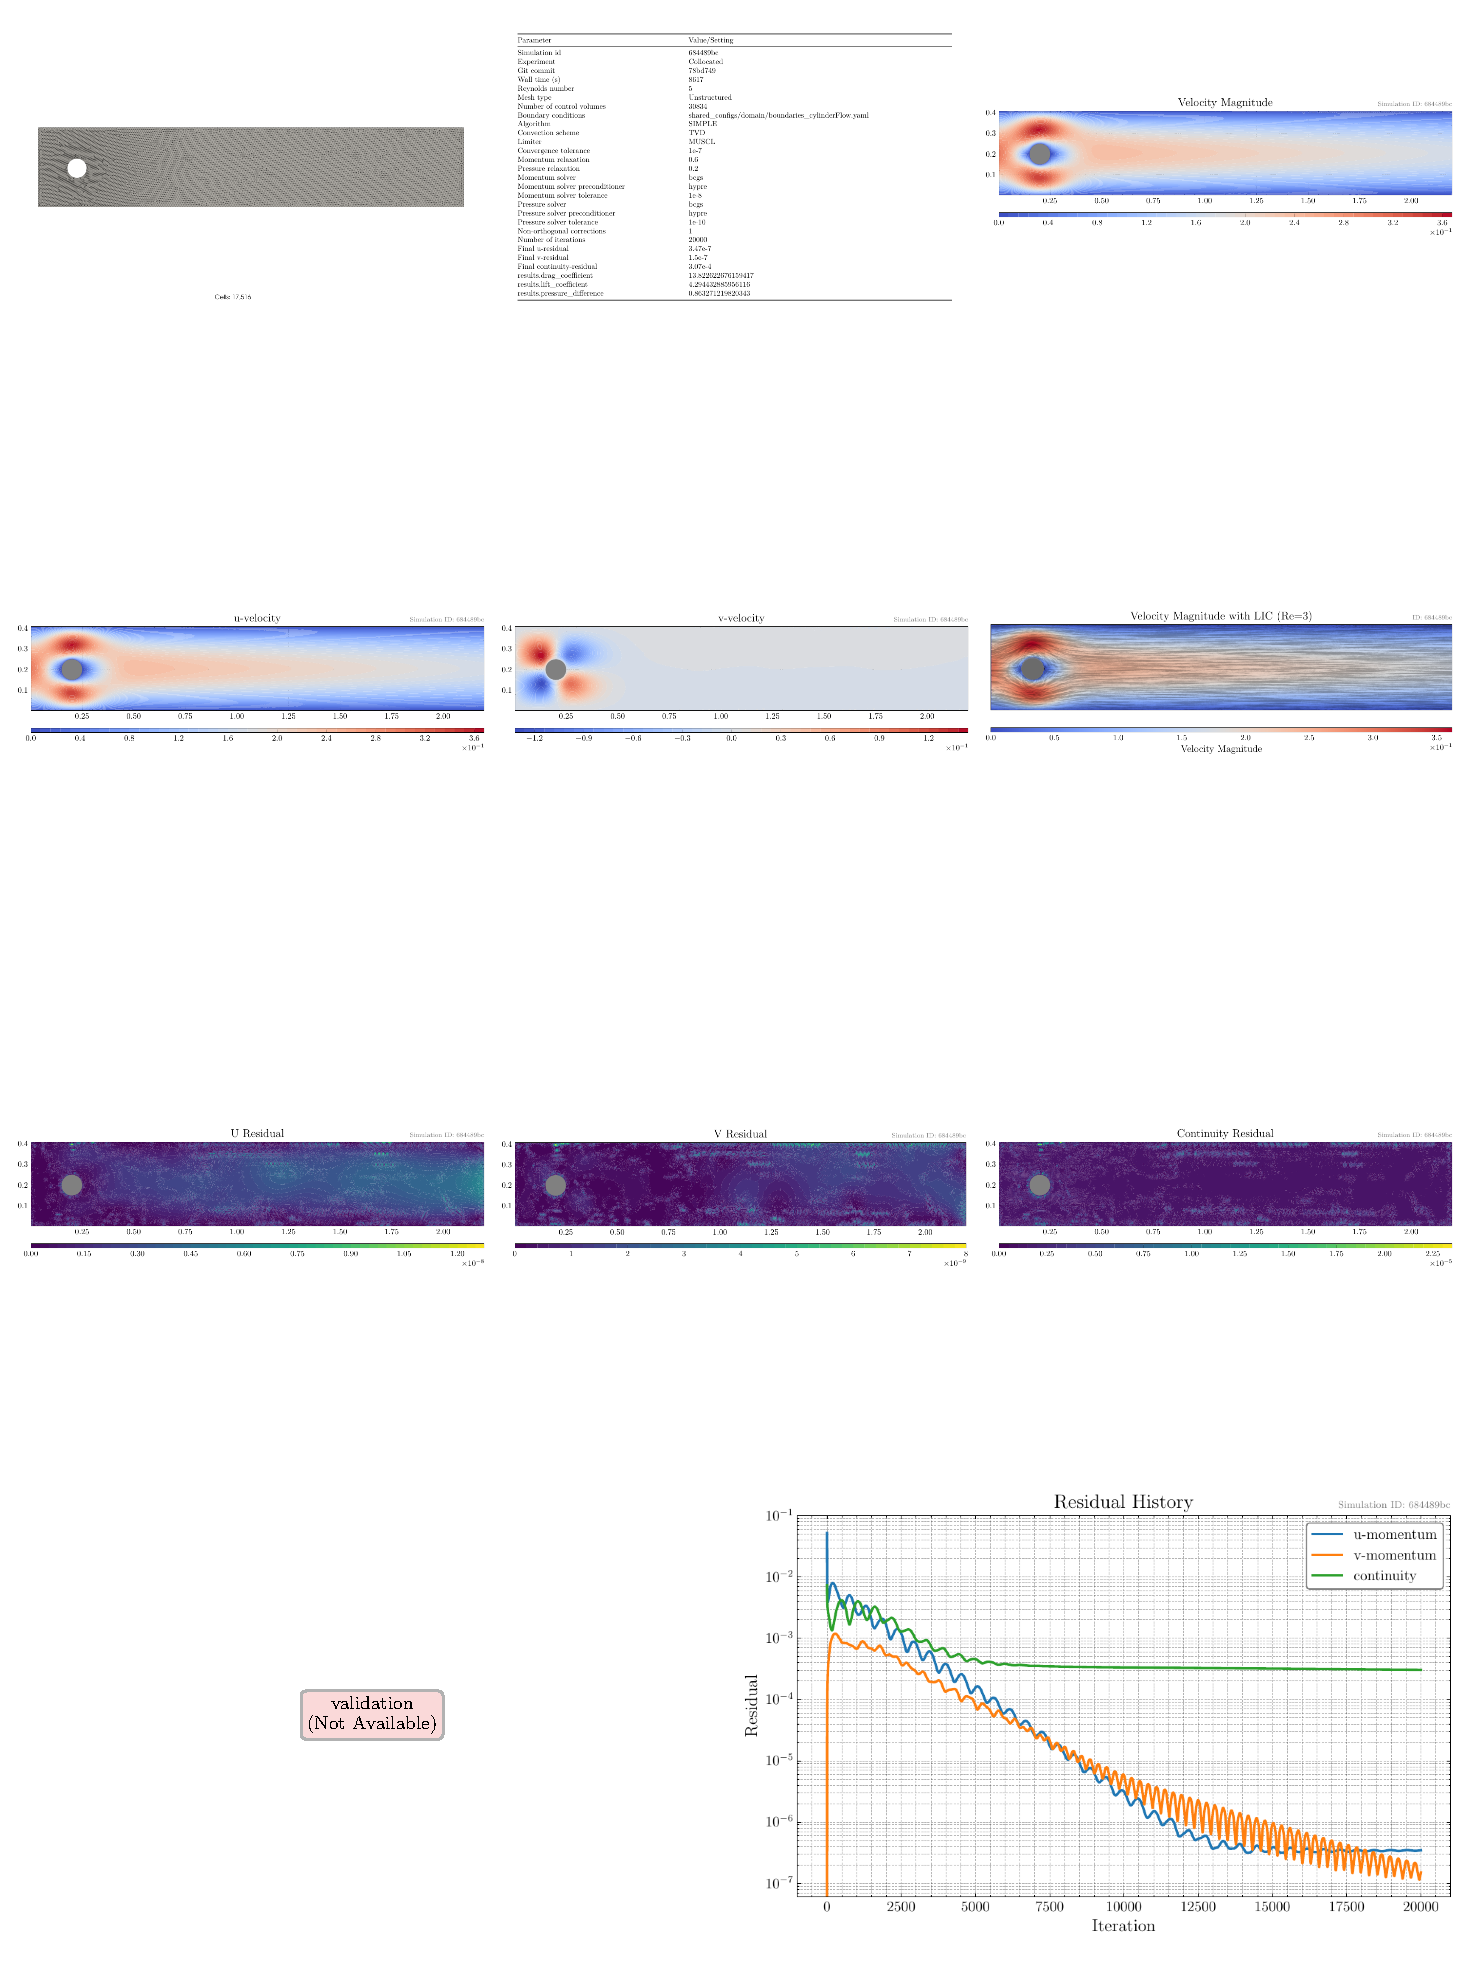
\includegraphics[width=0.85\linewidth]{AppendixPlots/cylinderFlow/Re_3/medium/cylinderFlow_Re3_unstructured_medium_TVD_684489bc.pdf}
    \caption{Cylinderflow simulation at Re=3 using unstructured medium mesh with TVD discretization scheme (Simulation ID: 684489bc)}
    \label{sim.cyl.re3.unstruct.med.tvd}
\end{figure}

\subsection*{Reynolds Number 5}
\addcontentsline{toc}{subsection}{Reynolds Number 5}
\label{subsec:cylinderflow_re5}

\subsubsection*{Fine Mesh}
\addcontentsline{toc}{subsubsection}{Fine Mesh}
\label{subsubsec:cylinderflow_re5_fine}

\paragraph*{Unstructured Mesh with TVD Scheme}
\addcontentsline{toc}{paragraph}{Unstructured Mesh with TVD Scheme}
\label{para:cylinderflow_re5_fine_unstructured_TVD}

\begin{figure}[H]
    \centering
    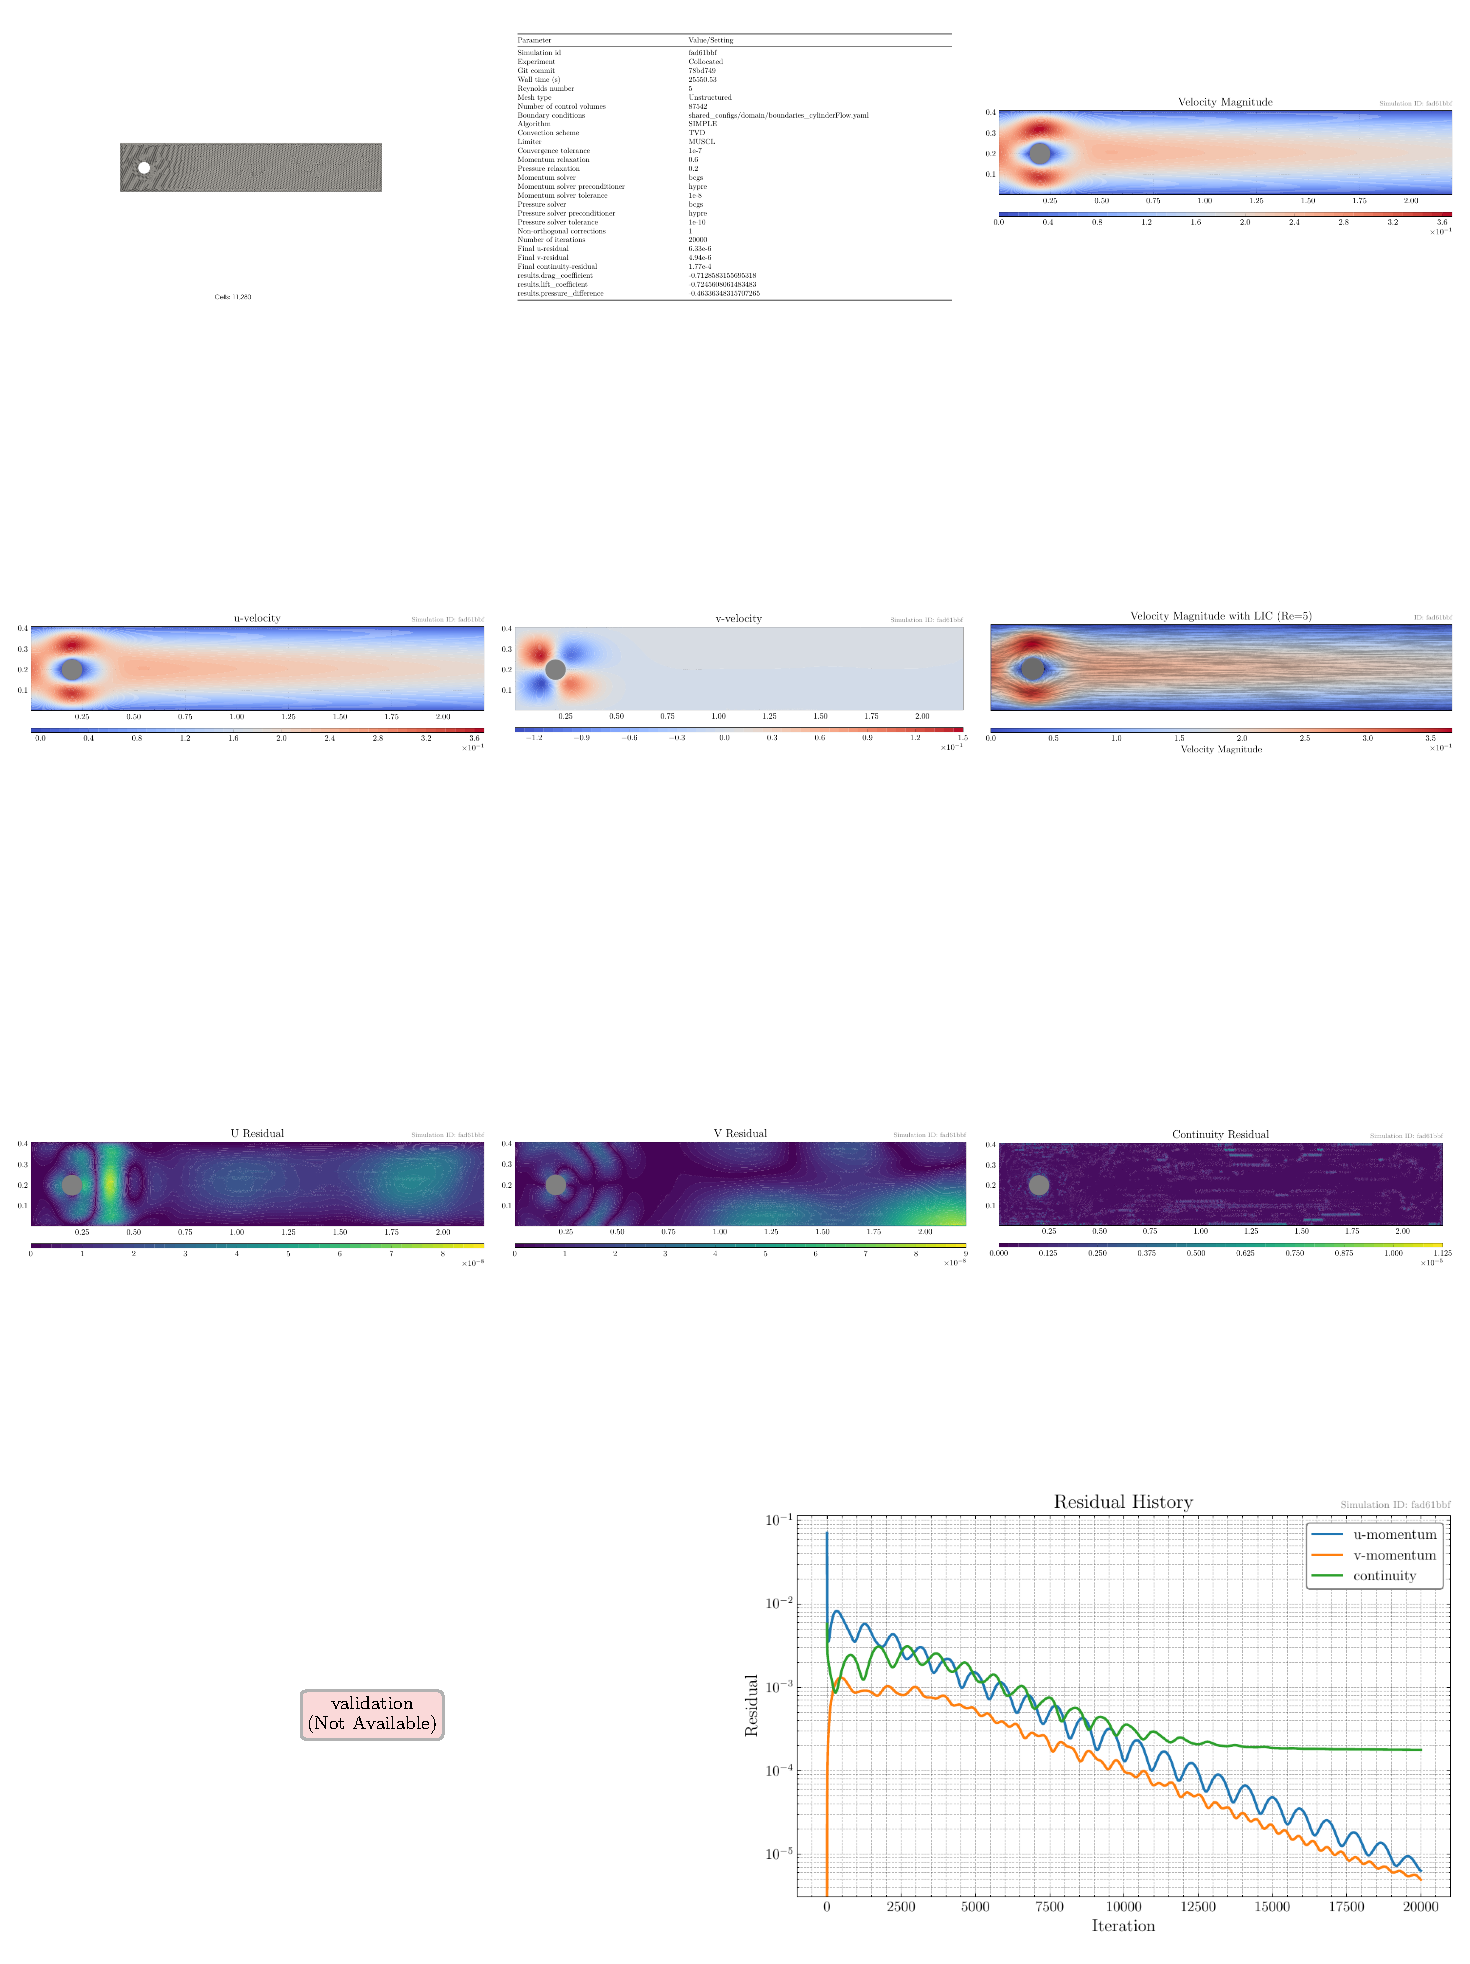
\includegraphics[width=0.85\linewidth]{AppendixPlots/cylinderFlow/Re_5/fine/cylinderFlow_Re5_unstructured_fine_TVD_fad61bbf.pdf}
    \caption{Cylinderflow simulation at Re=5 using unstructured fine mesh with TVD discretization scheme (Simulation ID: fad61bbf)}
    \label{sim.cyl.re5.unstruct.fine.tvd}
\end{figure}

\subsection*{Reynolds Number 20}
\addcontentsline{toc}{subsection}{Reynolds Number 20}
\label{subsec:cylinderflow_re20}

\subsubsection*{Coarse Mesh}
\addcontentsline{toc}{subsubsection}{Coarse Mesh}
\label{subsubsec:cylinderflow_re20_coarse}

\paragraph*{Unstructured Mesh with TVD Scheme}
\addcontentsline{toc}{paragraph}{Unstructured Mesh with TVD Scheme}
\label{para:cylinderflow_re20_coarse_unstructured_TVD}

\begin{figure}[H]
    \centering
    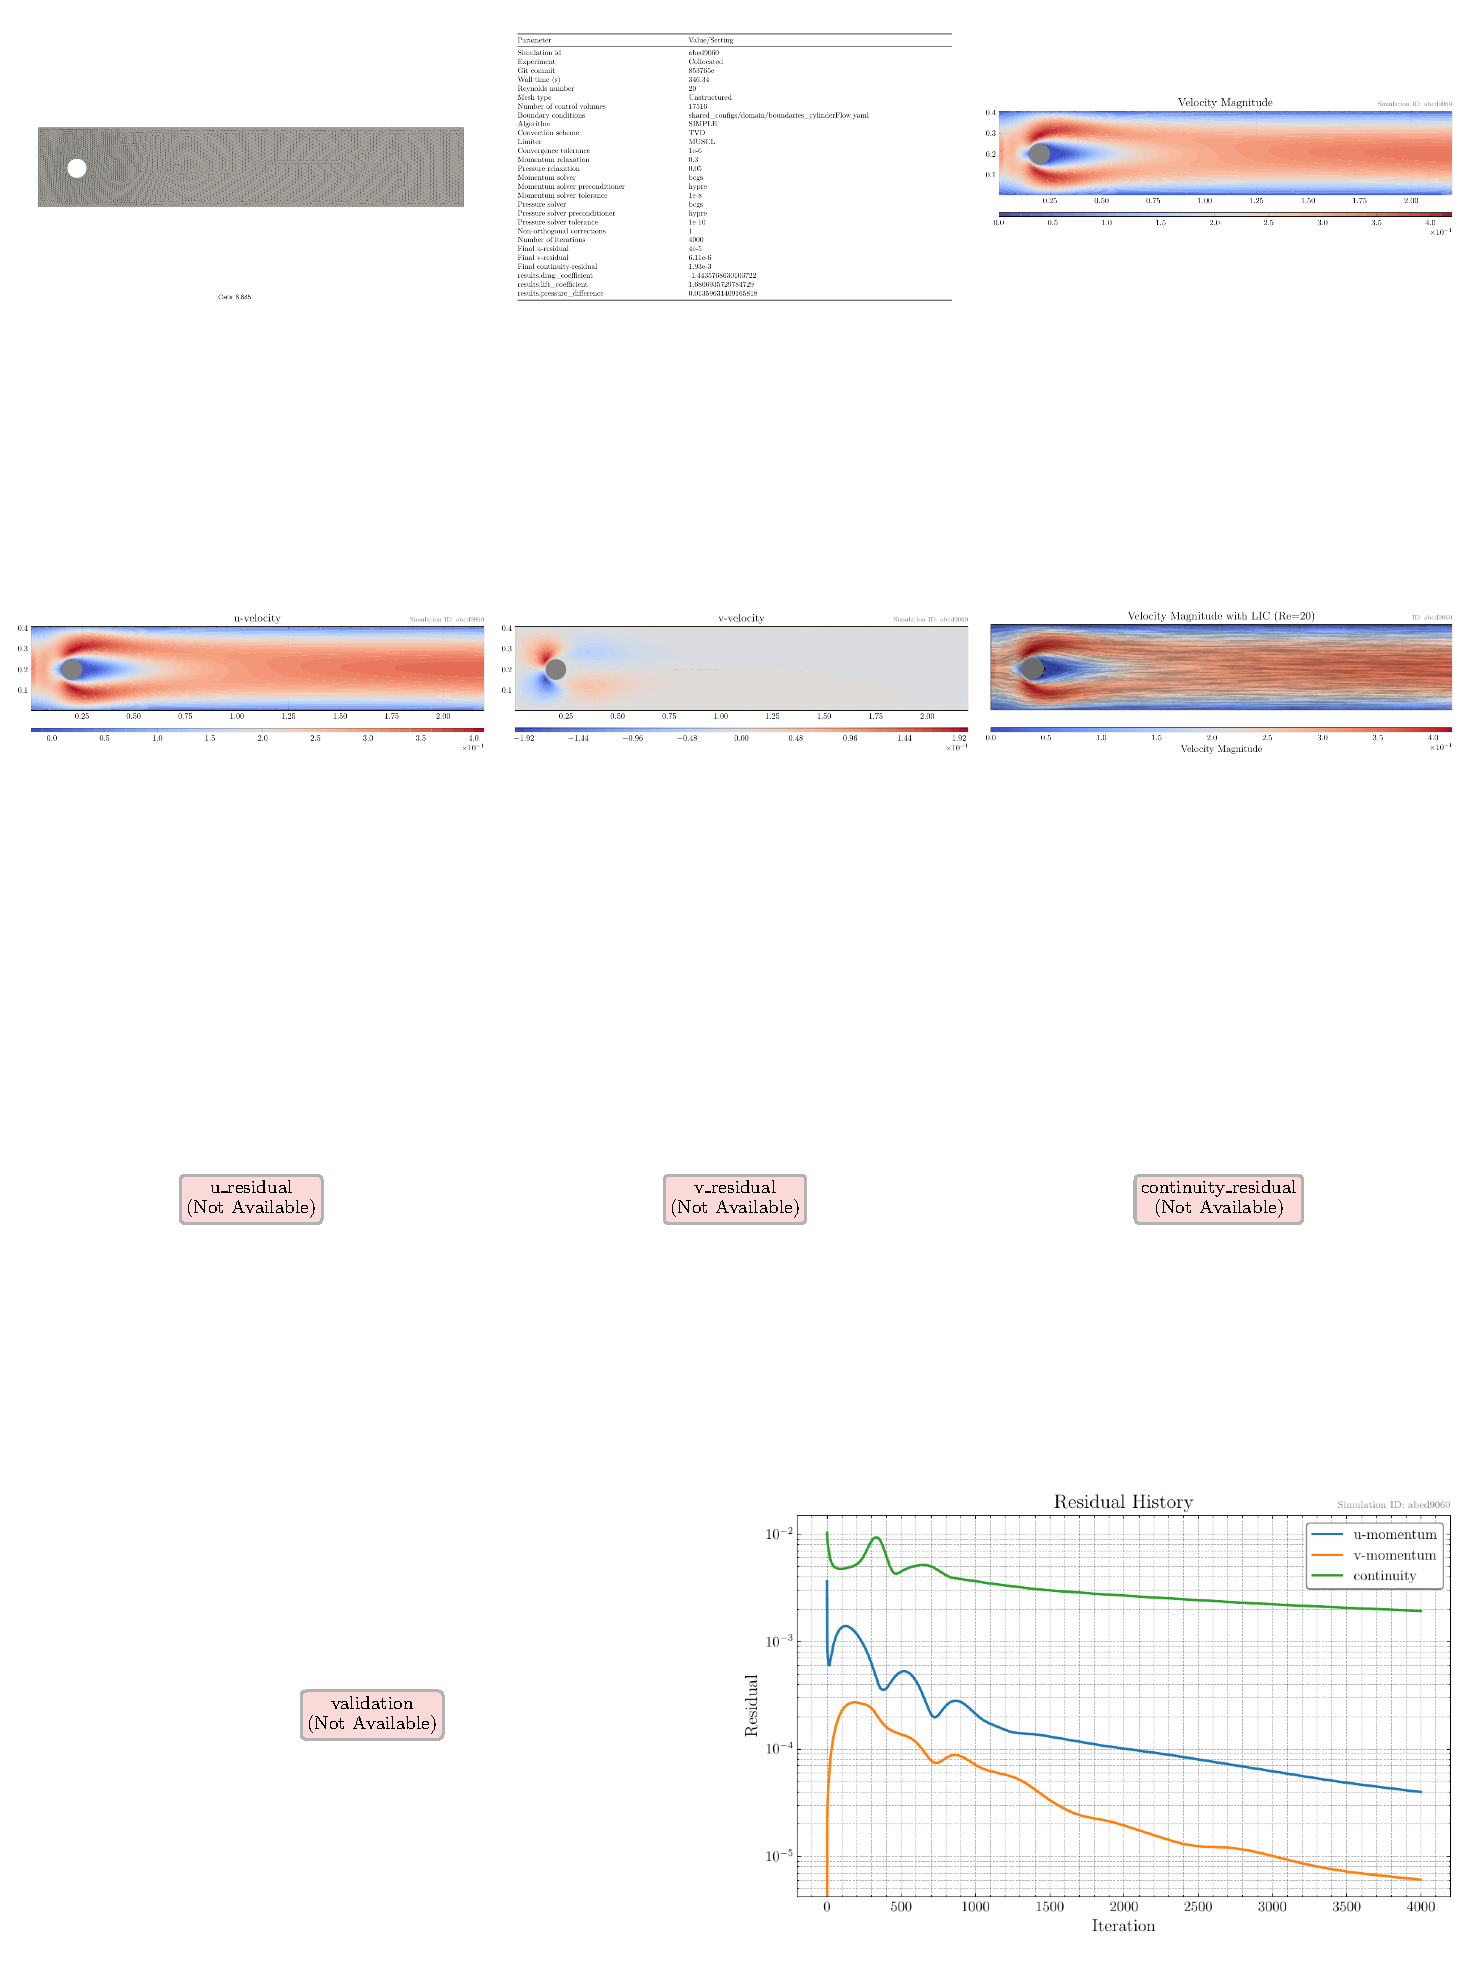
\includegraphics[width=0.85\linewidth]{AppendixPlots/cylinderFlow/Re_20/coarse/cylinderFlow_Re20_unstructured_coarse_TVD_abed9060.pdf}
    \caption{Cylinderflow simulation at Re=20 using unstructured coarse mesh with TVD discretization scheme (Simulation ID: abed9060)}
    \label{sim.cyl.re20.unstruct.coarse.tvd}
\end{figure}

\clearpage

\subsubsection*{Medium Mesh}
\addcontentsline{toc}{subsubsection}{Medium Mesh}
\label{subsubsec:cylinderflow_re20_medium}

\paragraph*{Unstructured Mesh with TVD Scheme}
\addcontentsline{toc}{paragraph}{Unstructured Mesh with TVD Scheme}
\label{para:cylinderflow_re20_medium_unstructured_TVD}

\begin{figure}[H]
    \centering
    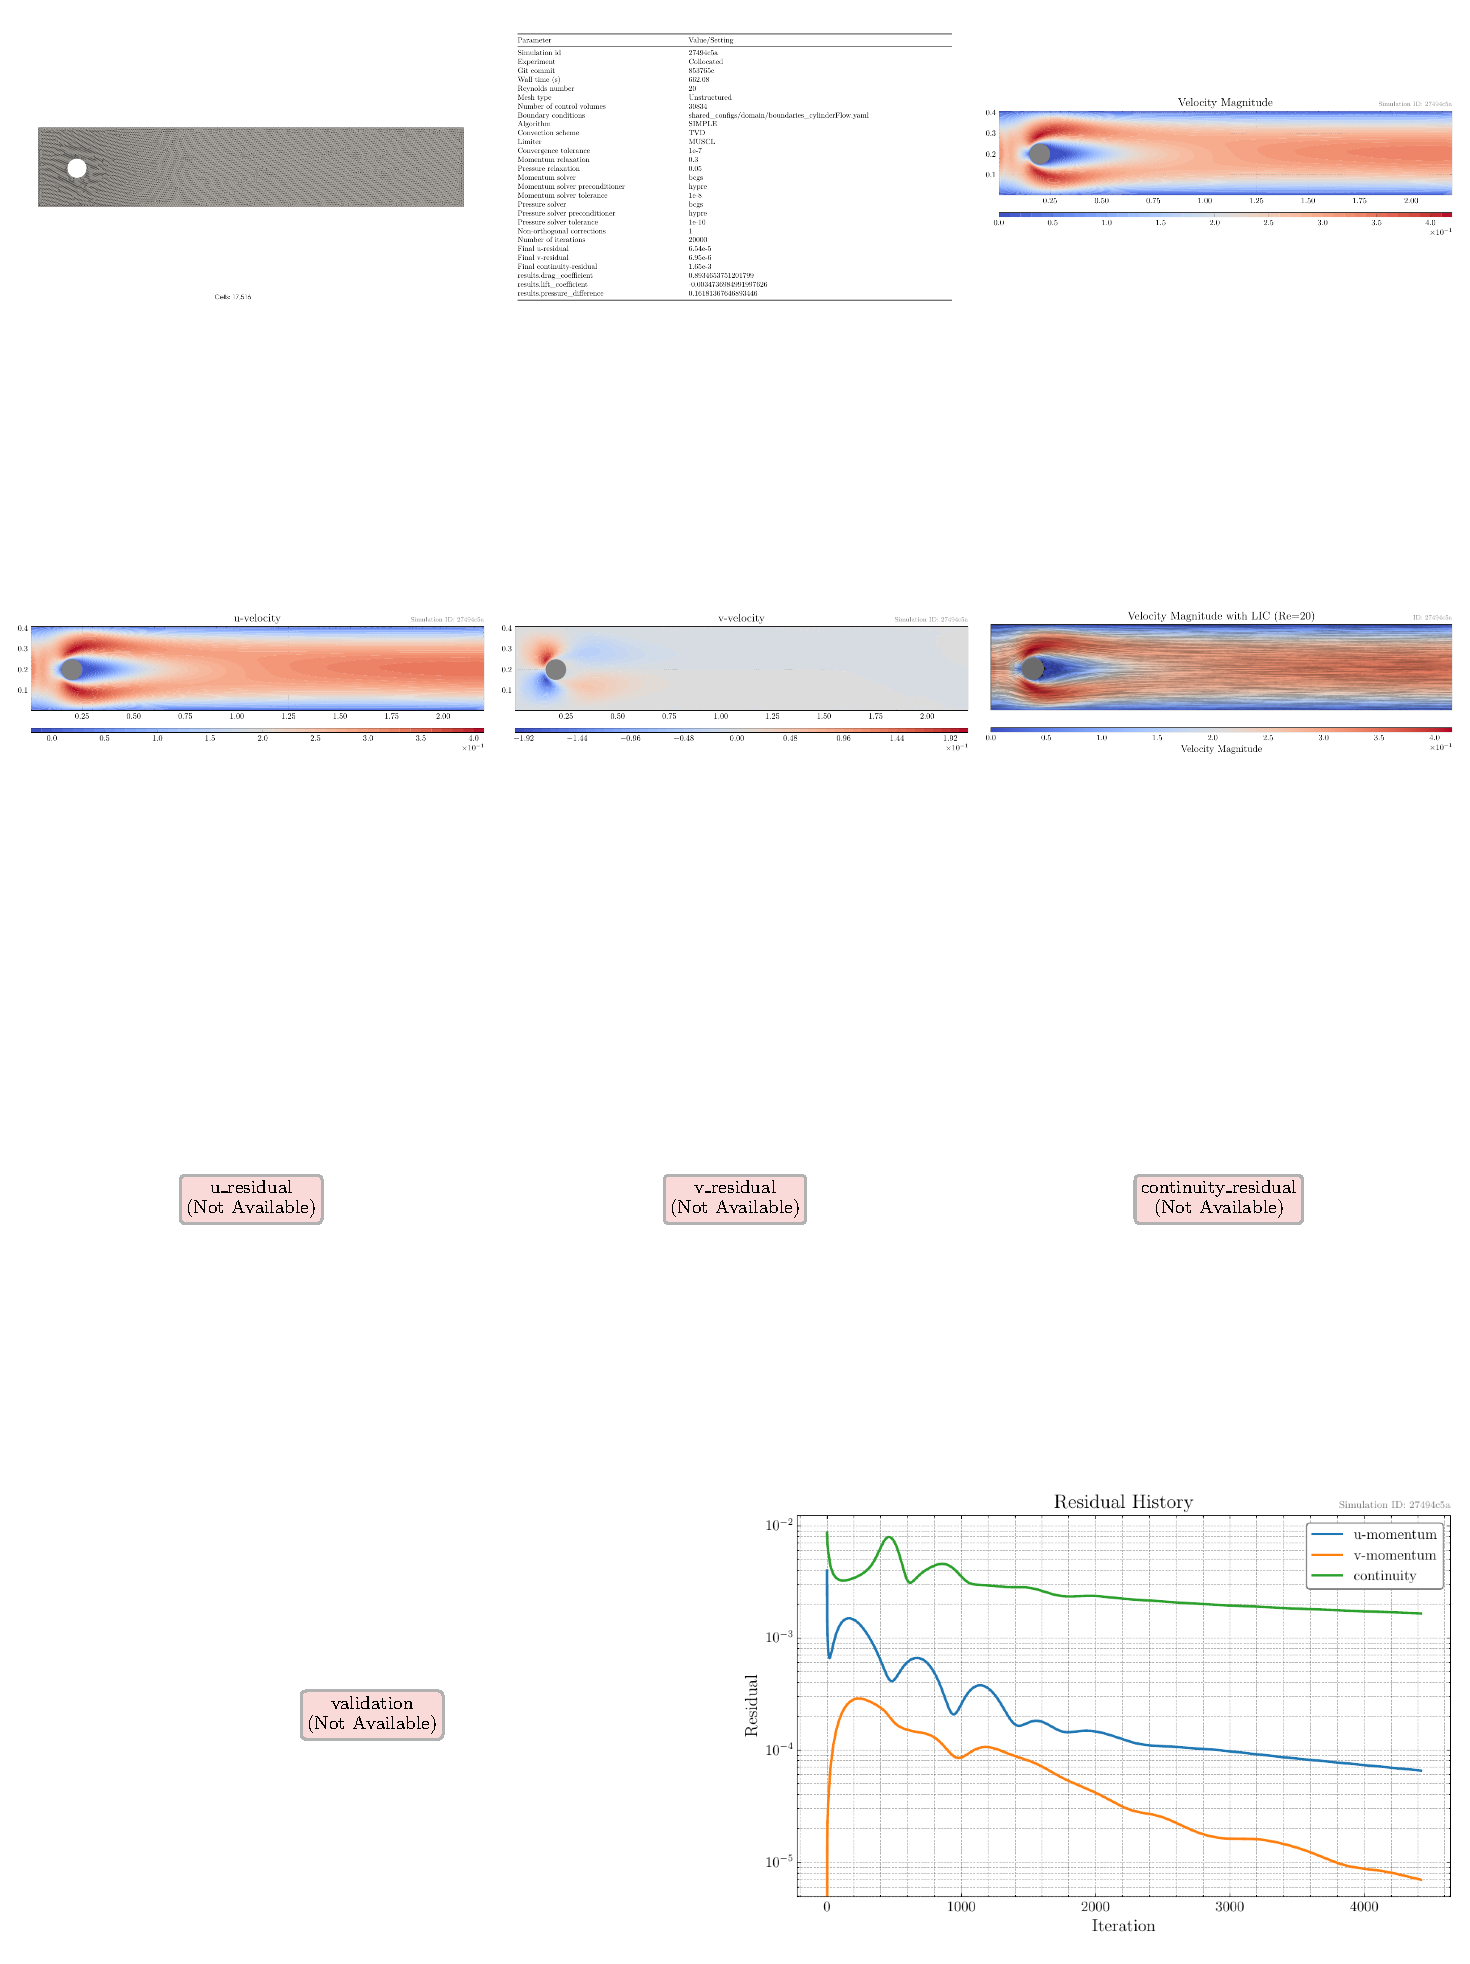
\includegraphics[width=0.85\linewidth]{AppendixPlots/cylinderFlow/Re_20/medium/cylinderFlow_Re20_unstructured_medium_TVD_27494c5a.pdf}
    \caption{Cylinderflow simulation at Re=20 using unstructured medium mesh with TVD discretization scheme (Simulation ID: 27494c5a)}
    \label{sim.cyl.re20.unstruct.med.tvd}
\end{figure}

\clearpage

\subsubsection*{Fine Mesh}
\addcontentsline{toc}{subsubsection}{Fine Mesh}
\label{subsubsec:cylinderflow_re20_fine}

\paragraph*{Unstructured Mesh with TVD Scheme}
\addcontentsline{toc}{paragraph}{Unstructured Mesh with TVD Scheme}
\label{para:cylinderflow_re20_fine_unstructured_TVD}

\begin{figure}[H]
    \centering
    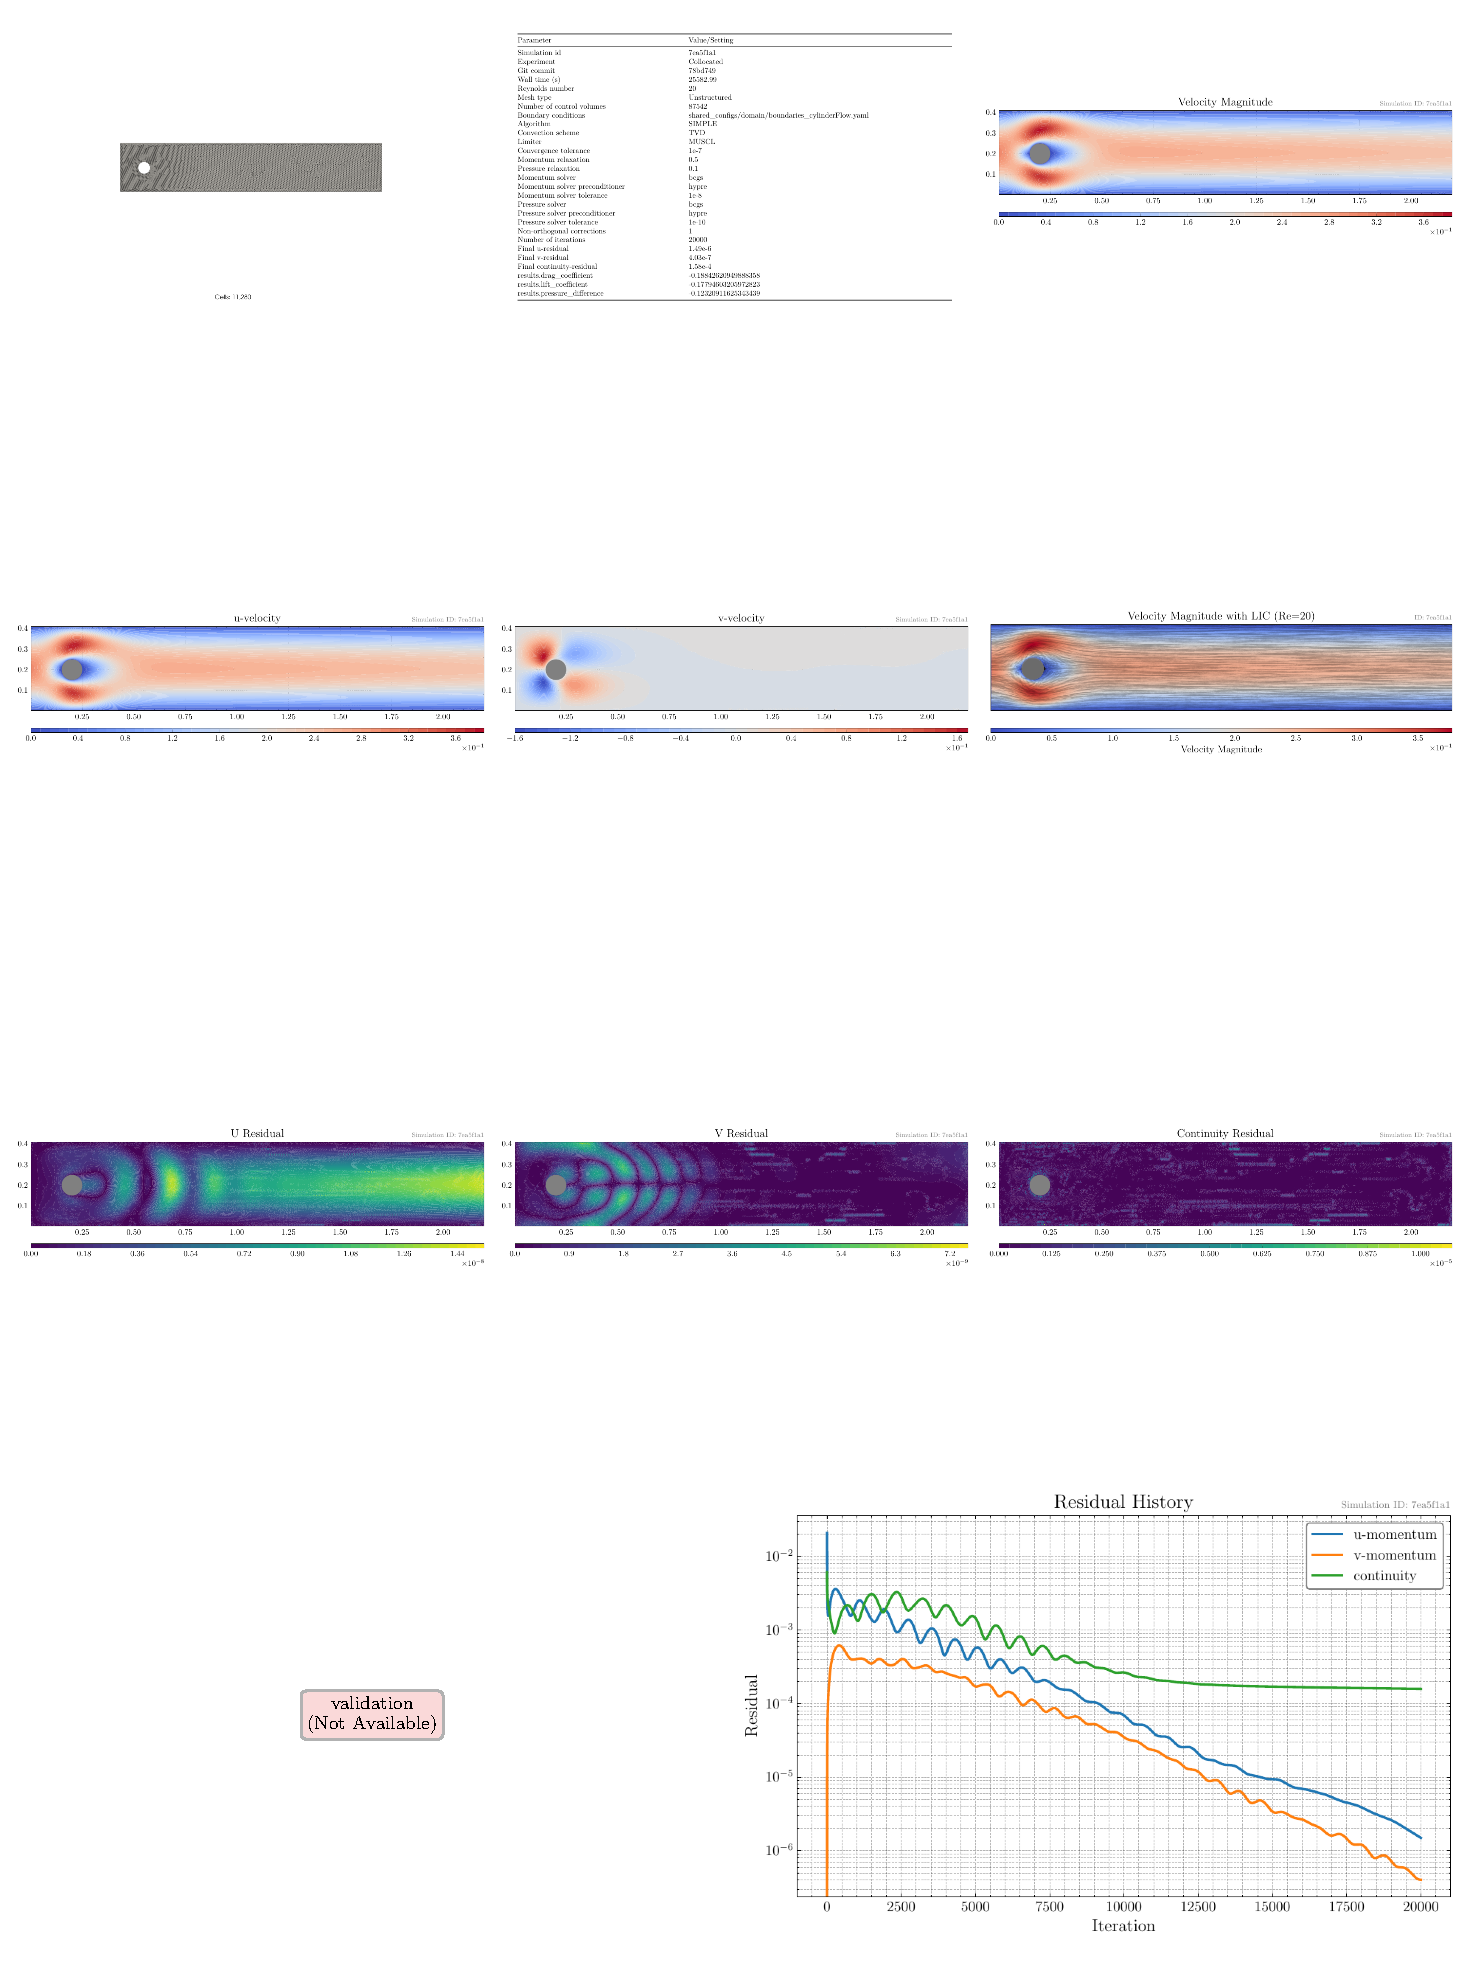
\includegraphics[width=0.85\linewidth]{AppendixPlots/cylinderFlow/Re_20/fine/cylinderFlow_Re20_unstructured_fine_TVD_7ea5f1a1.pdf}
    \caption{Cylinderflow simulation at Re=20 using unstructured fine mesh with TVD discretization scheme (Simulation ID: 7ea5f1a1)}
    \label{sim.cyl.re20.unstruct.fine.tvd}
\end{figure}

\subsection*{Reynolds Number 100}
\addcontentsline{toc}{subsection}{Reynolds Number 100}
\label{subsec:cylinderflow_re100}

\subsubsection*{Medium Mesh}
\addcontentsline{toc}{subsubsection}{Medium Mesh}
\label{subsubsec:cylinderflow_re100_medium}

\paragraph*{Unstructured Mesh with TVD Scheme}
\addcontentsline{toc}{paragraph}{Unstructured Mesh with TVD Scheme}
\label{para:cylinderflow_re100_medium_unstructured_TVD}

\begin{figure}[H]
    \centering
    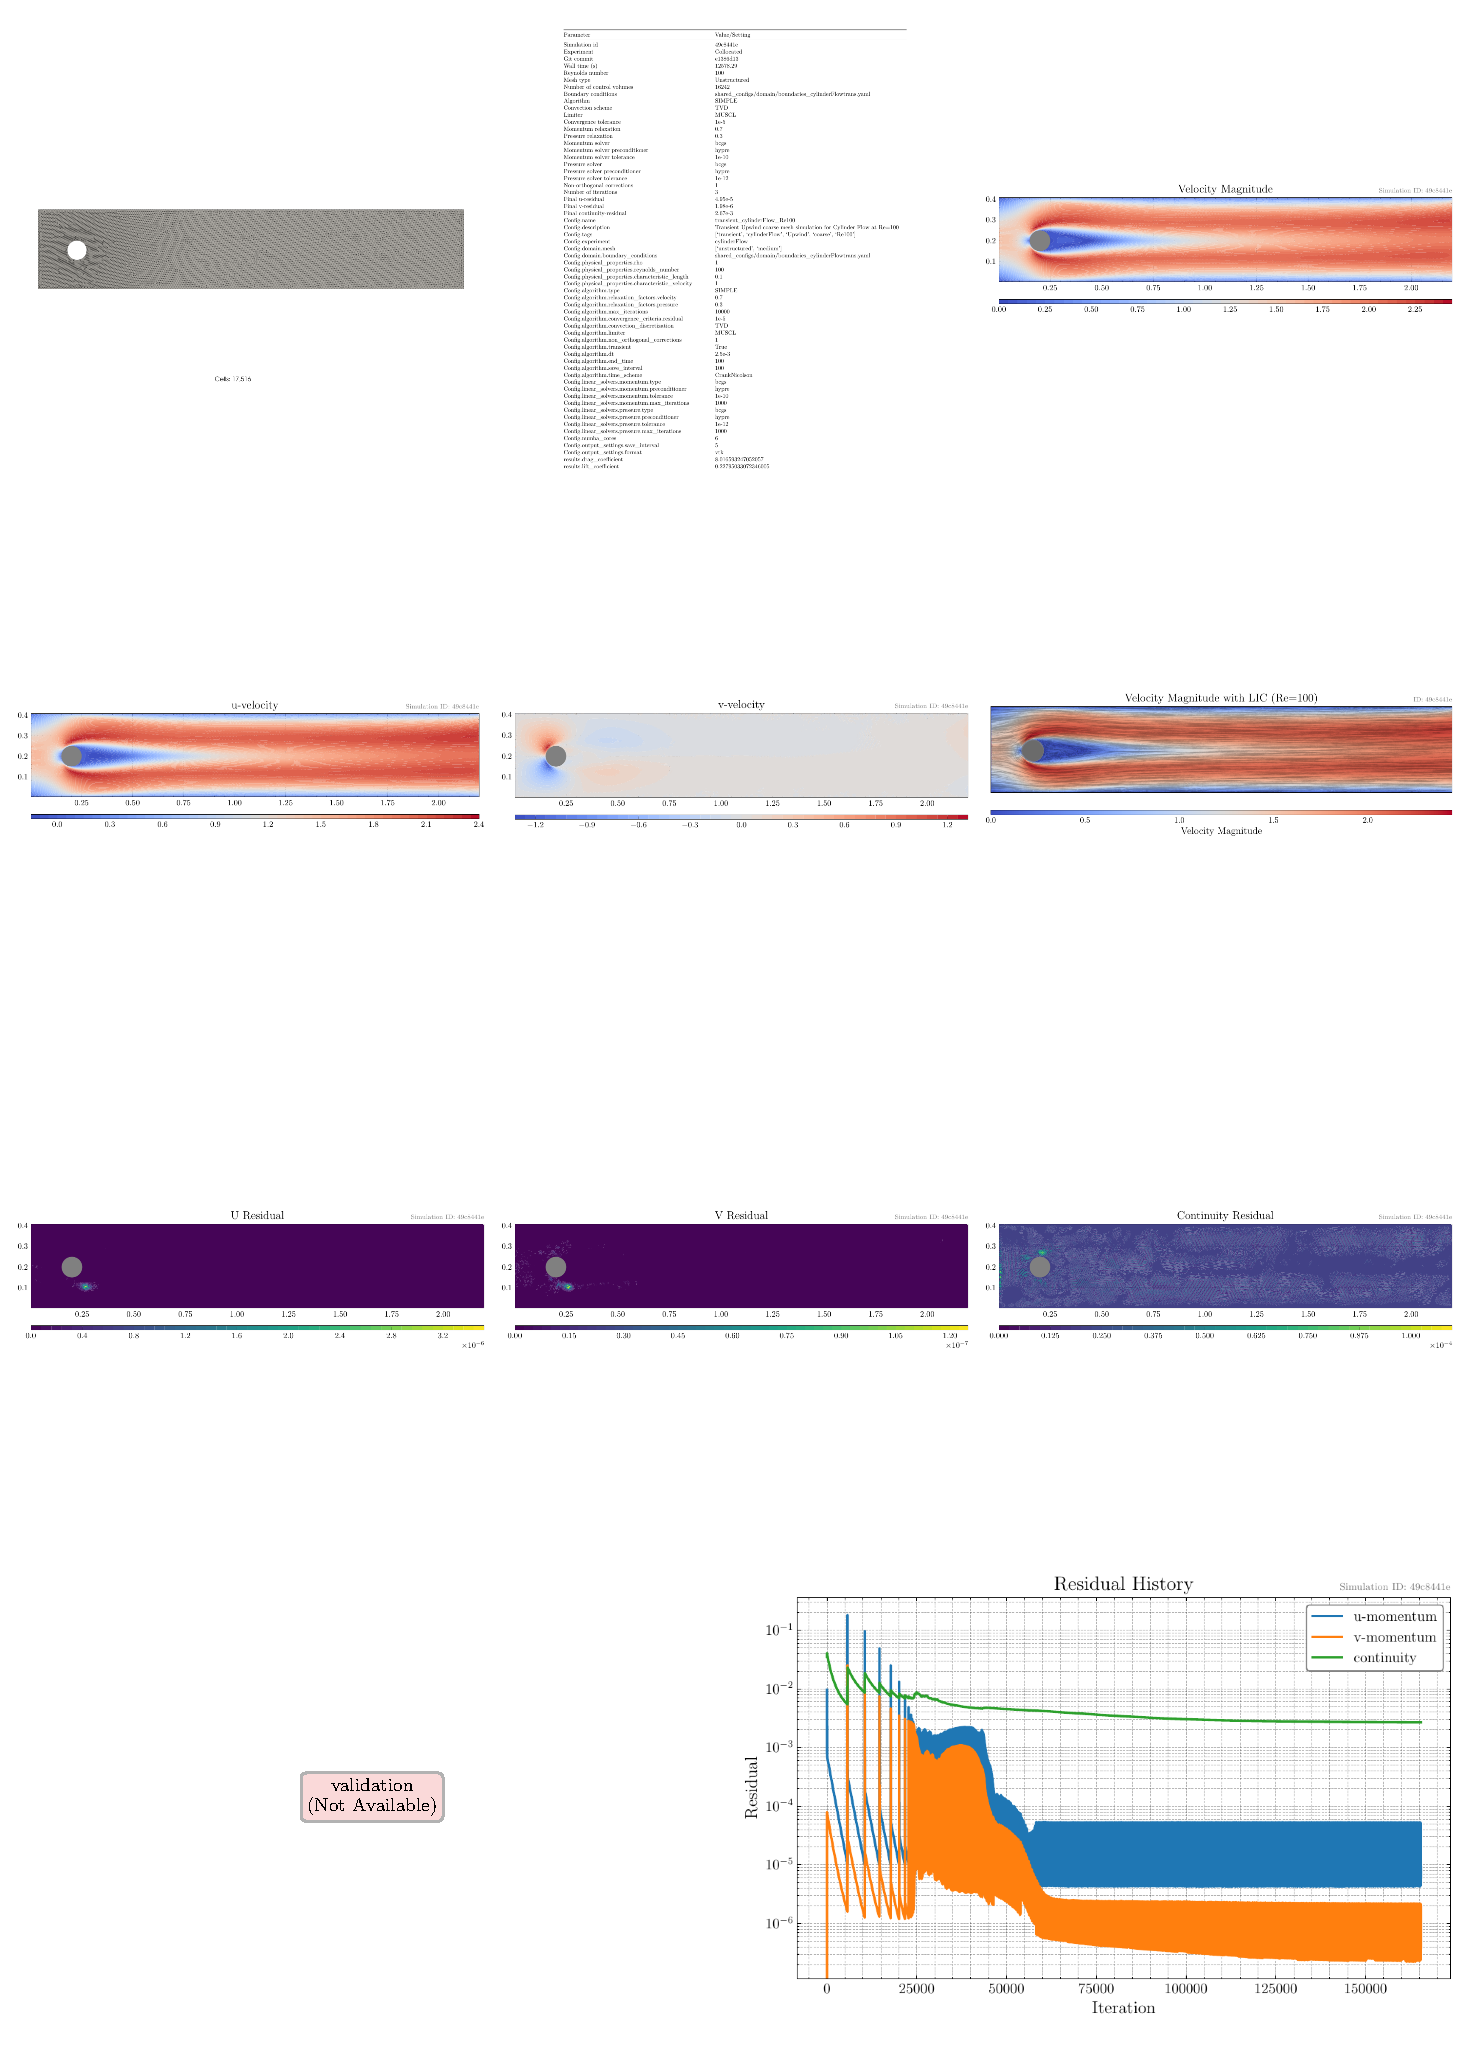
\includegraphics[width=0.85\linewidth]{AppendixPlots/cylinderFlow/Re_100/medium/cylinderFlow_Re100_unstructured_medium_TVD_49c8441e.pdf}
    \caption{Cylinderflow simulation at Re=100 using unstructured medium mesh with TVD discretization scheme (Simulation ID: 49c8441e)}
    \label{sim.cyl.re100.unstruct.med.tvd}
\end{figure}

\clearpage

\subsubsection*{Fine Mesh}
\addcontentsline{toc}{subsubsection}{Fine Mesh}
\label{subsubsec:cylinderflow_re100_fine}

\paragraph*{Unstructured Mesh with TVD Scheme}
\addcontentsline{toc}{paragraph}{Unstructured Mesh with TVD Scheme}
\label{para:cylinderflow_re100_fine_unstructured_TVD}

\begin{figure}[H]
    \centering
    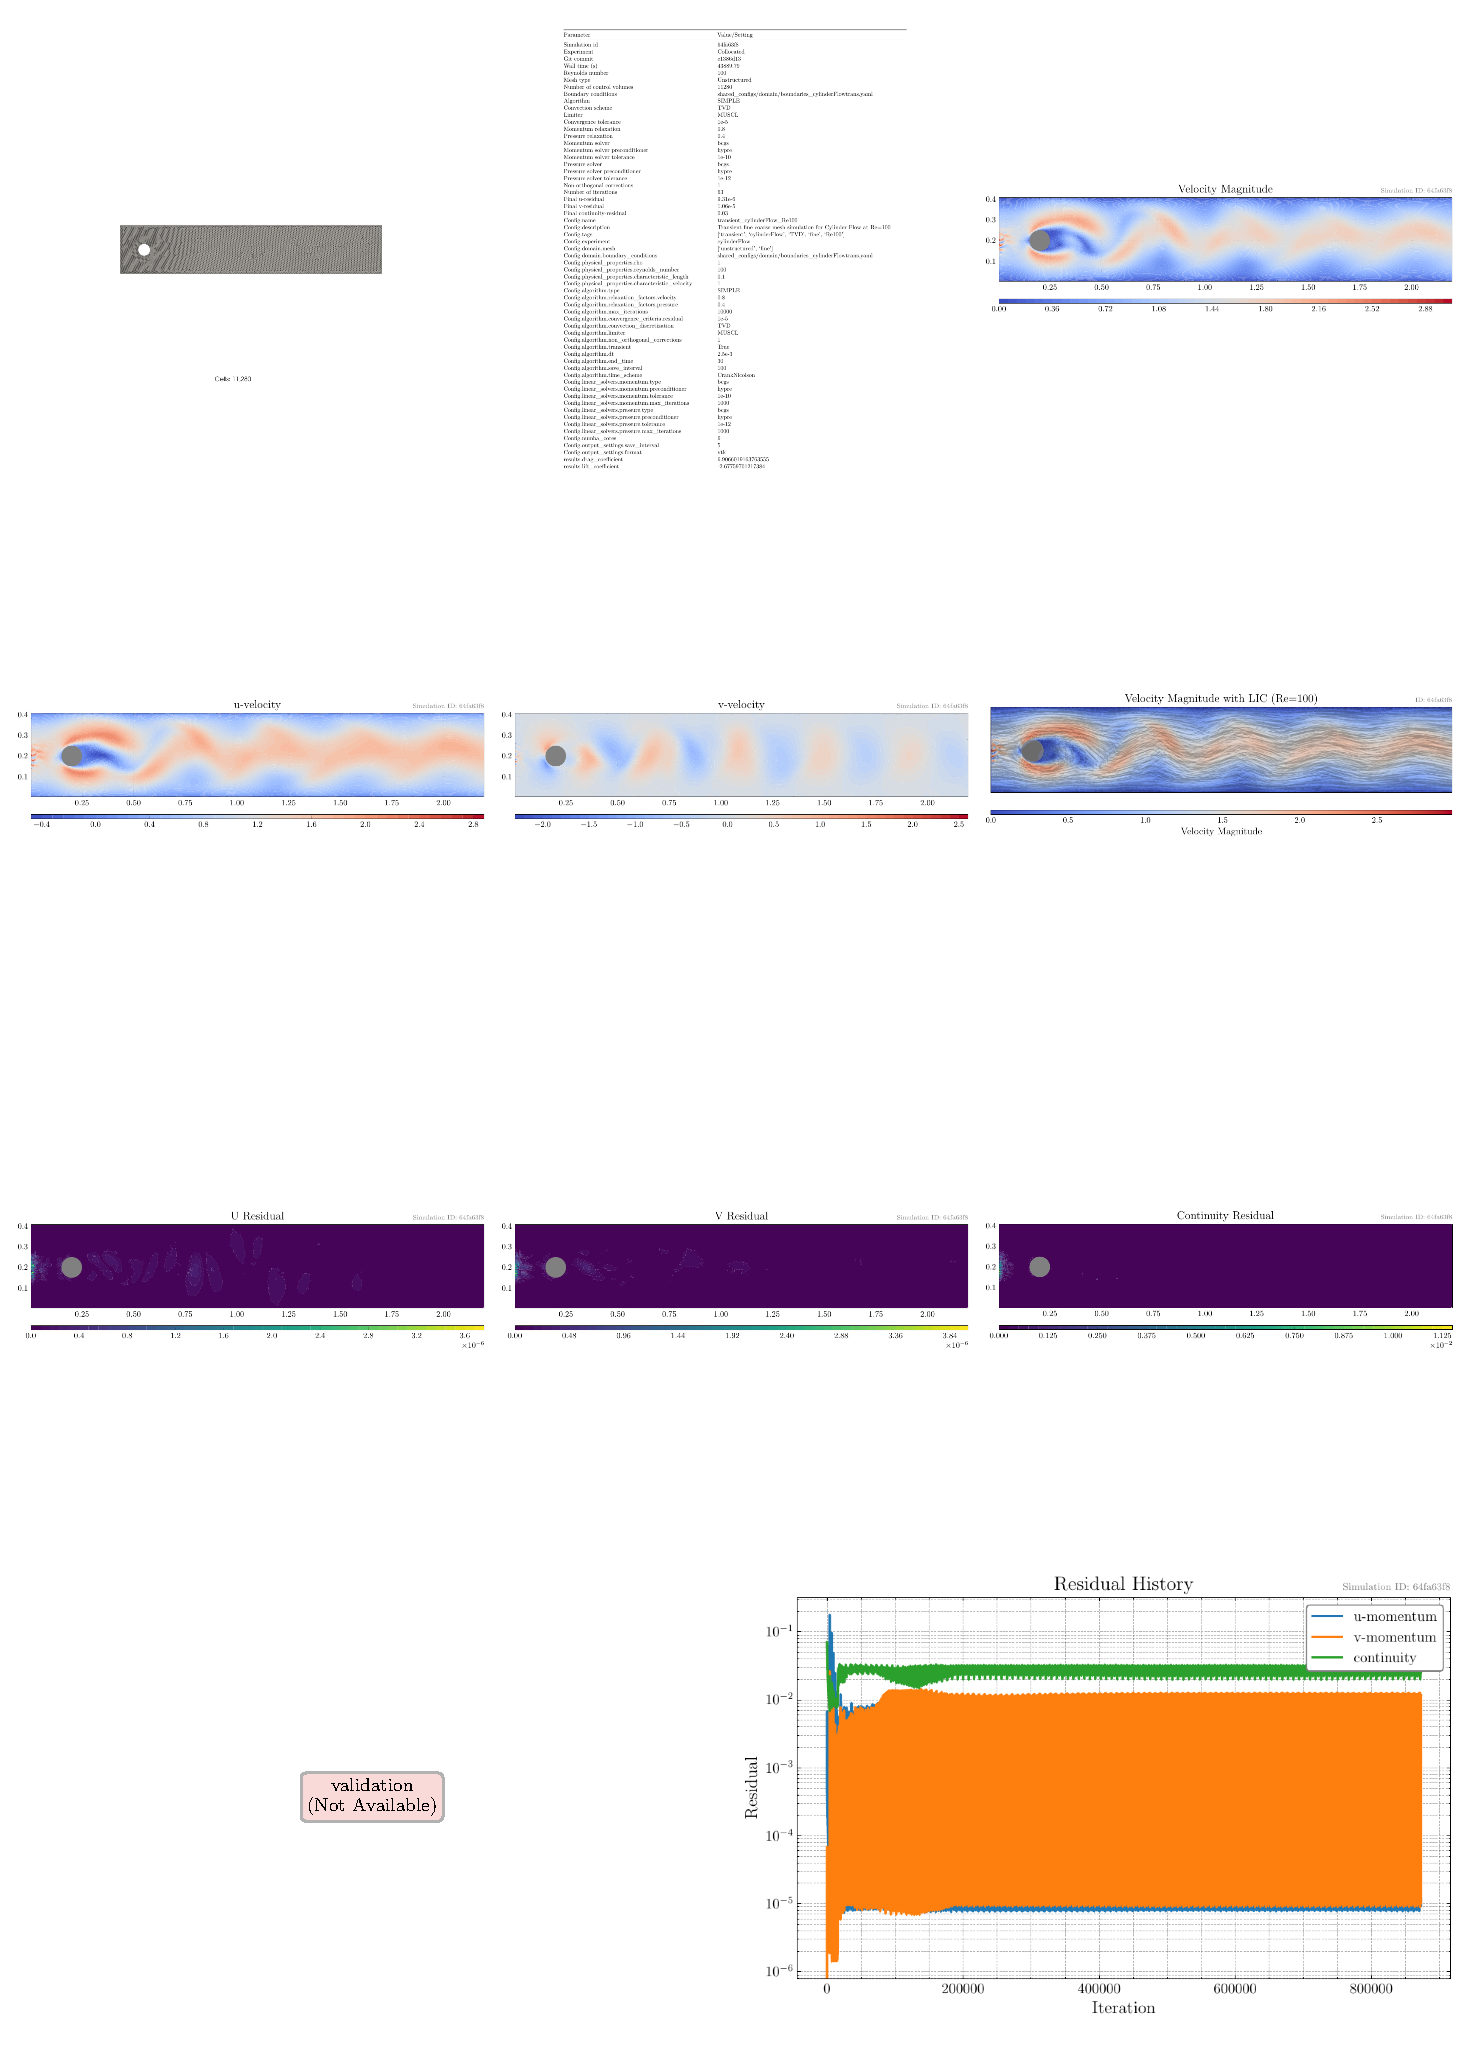
\includegraphics[width=0.85\linewidth]{AppendixPlots/cylinderFlow/Re_100/fine/cylinderFlow_Re100_unstructured_fine_TVD_64fa63f8.pdf}
    \caption{Cylinderflow simulation at Re=100 using unstructured fine mesh with TVD discretization scheme (Simulation ID: 64fa63f8)}
    \label{sim.cyl.re100.unstruct.fine.tvd}
\end{figure}

\subsection*{Reynolds Number 125}
\addcontentsline{toc}{subsection}{Reynolds Number 125}
\label{subsec:cylinderflow_re125}

\subsubsection*{Medium Mesh}
\addcontentsline{toc}{subsubsection}{Medium Mesh}
\label{subsubsec:cylinderflow_re125_medium}

\paragraph*{Unstructured Mesh with TVD Scheme}
\addcontentsline{toc}{paragraph}{Unstructured Mesh with TVD Scheme}
\label{para:cylinderflow_re125_medium_unstructured_TVD}

\begin{figure}[H]
    \centering
    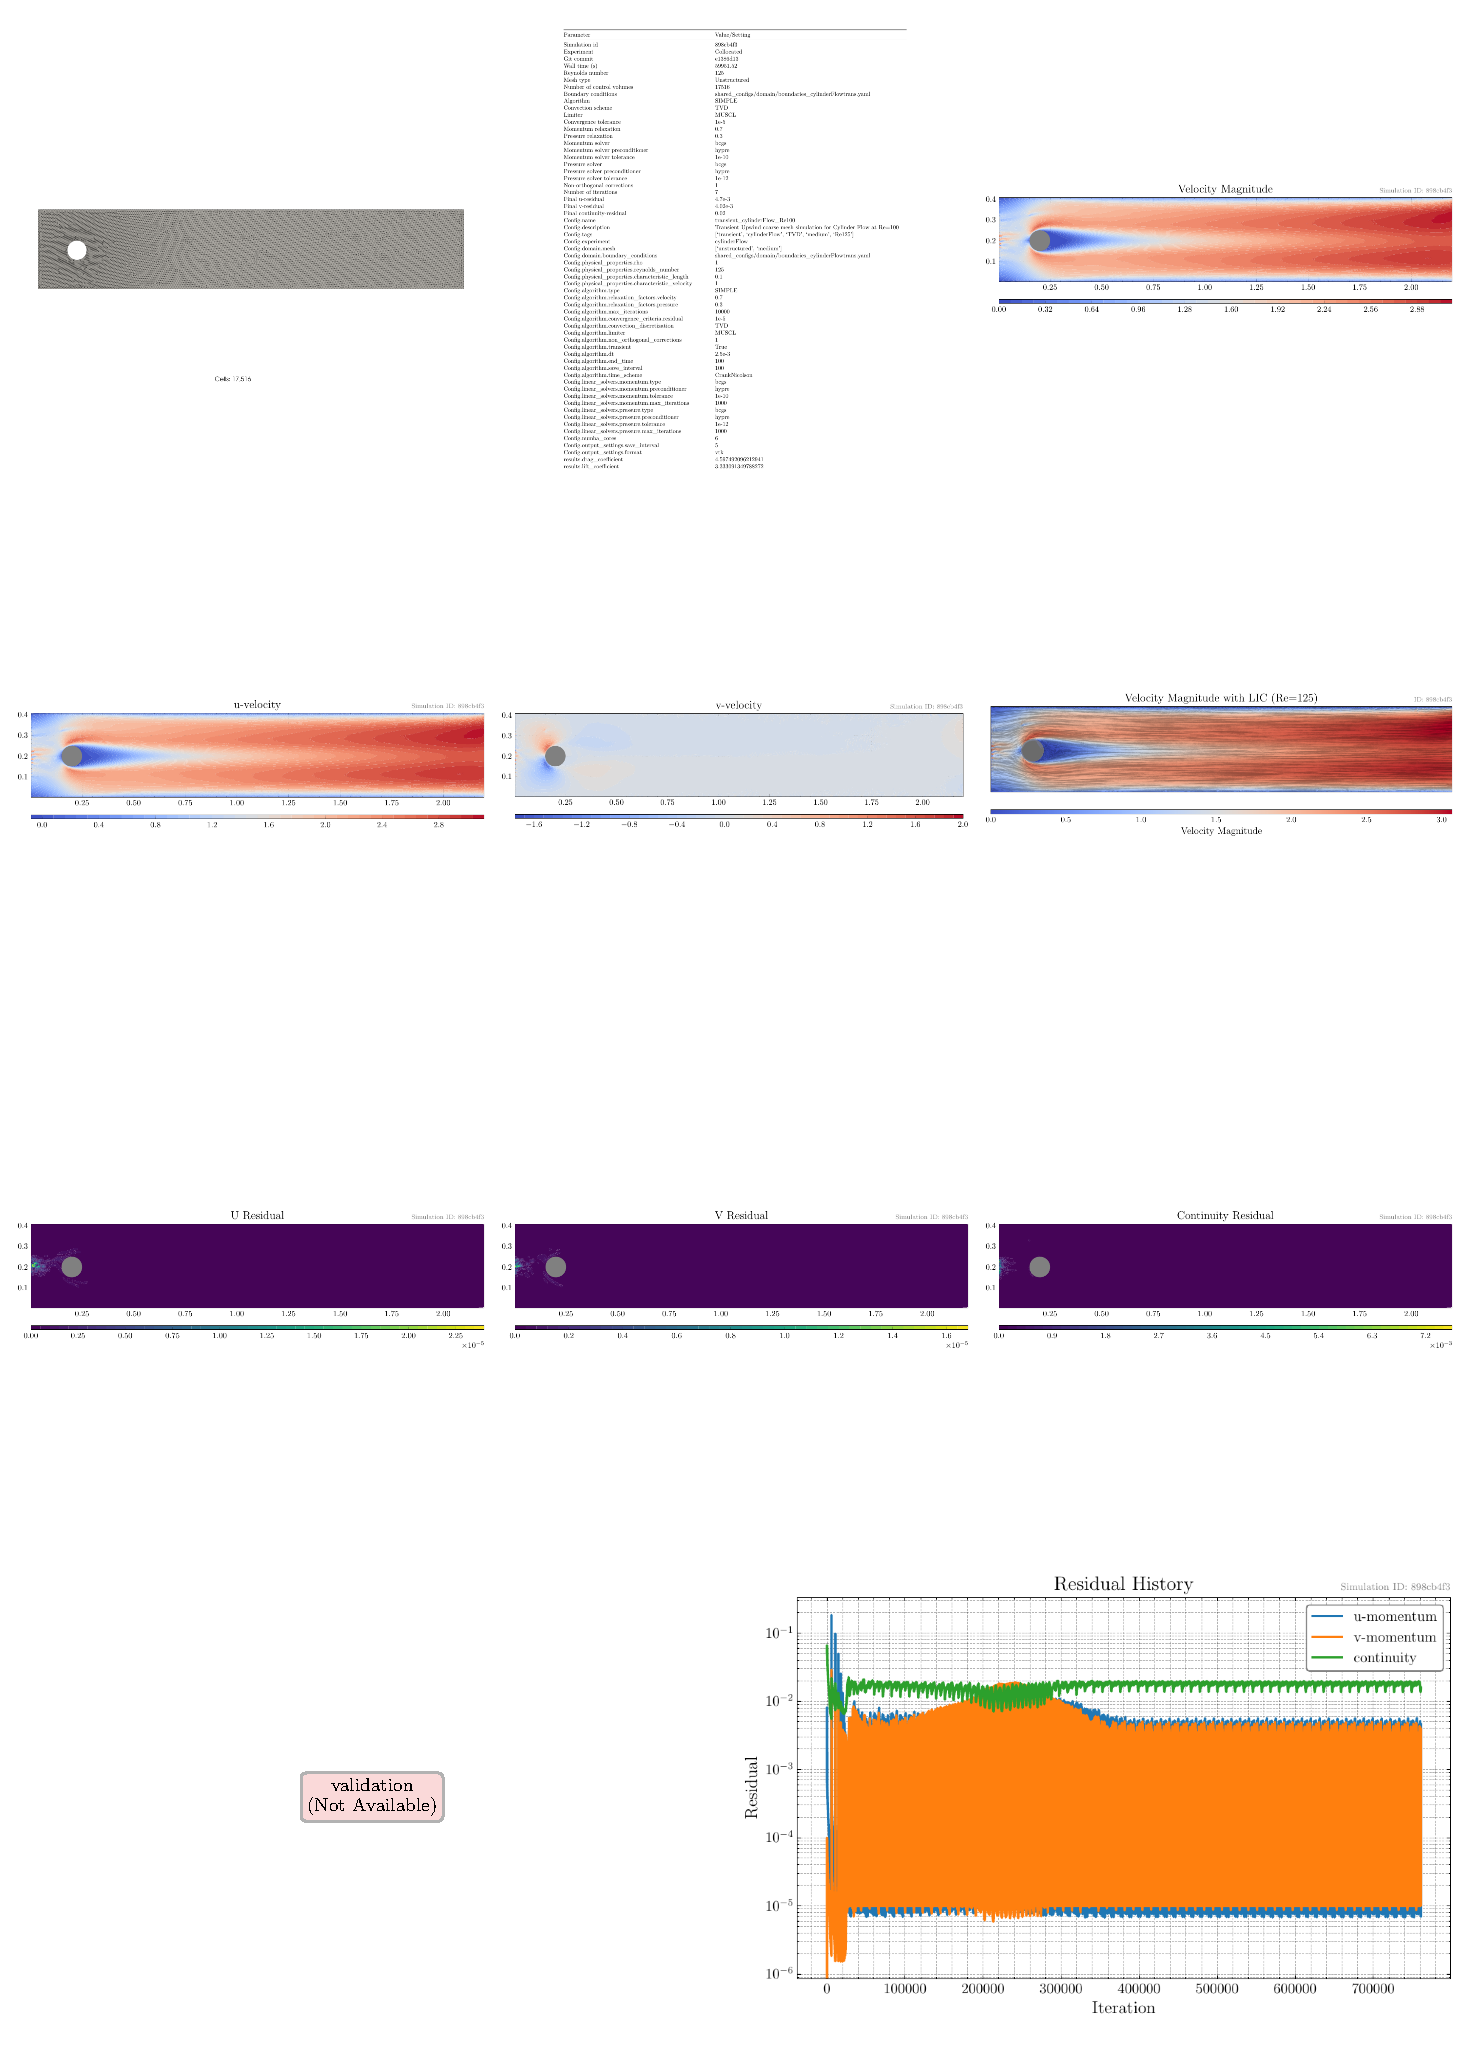
\includegraphics[width=0.85\linewidth]{AppendixPlots/cylinderFlow/Re_125/medium/cylinderFlow_Re125_unstructured_medium_TVD_898cb4f3.pdf}
    \caption{Cylinderflow simulation at Re=125 using unstructured medium mesh with TVD discretization scheme (Simulation ID: 898cb4f3)}
    \label{sim.cyl.re125.unstruct.med.tvd}
\end{figure}

\clearpage

\section*{Liddrivencavity Results}
\addcontentsline{toc}{section}{Liddrivencavity Results}
\label{sec:liddrivencavity_results}

\subsection*{Reynolds Number 100}
\addcontentsline{toc}{subsection}{Reynolds Number 100}
\label{subsec:liddrivencavity_re100}

\subsubsection*{Coarse Mesh}
\addcontentsline{toc}{subsubsection}{Coarse Mesh}
\label{subsubsec:liddrivencavity_re100_coarse}

\paragraph*{Uniform Mesh with QUICK Scheme}
\addcontentsline{toc}{paragraph}{Uniform Mesh with QUICK Scheme}
\label{para:liddrivencavity_re100_coarse_uniform_QUICK}

\begin{figure}[H]
    \centering
    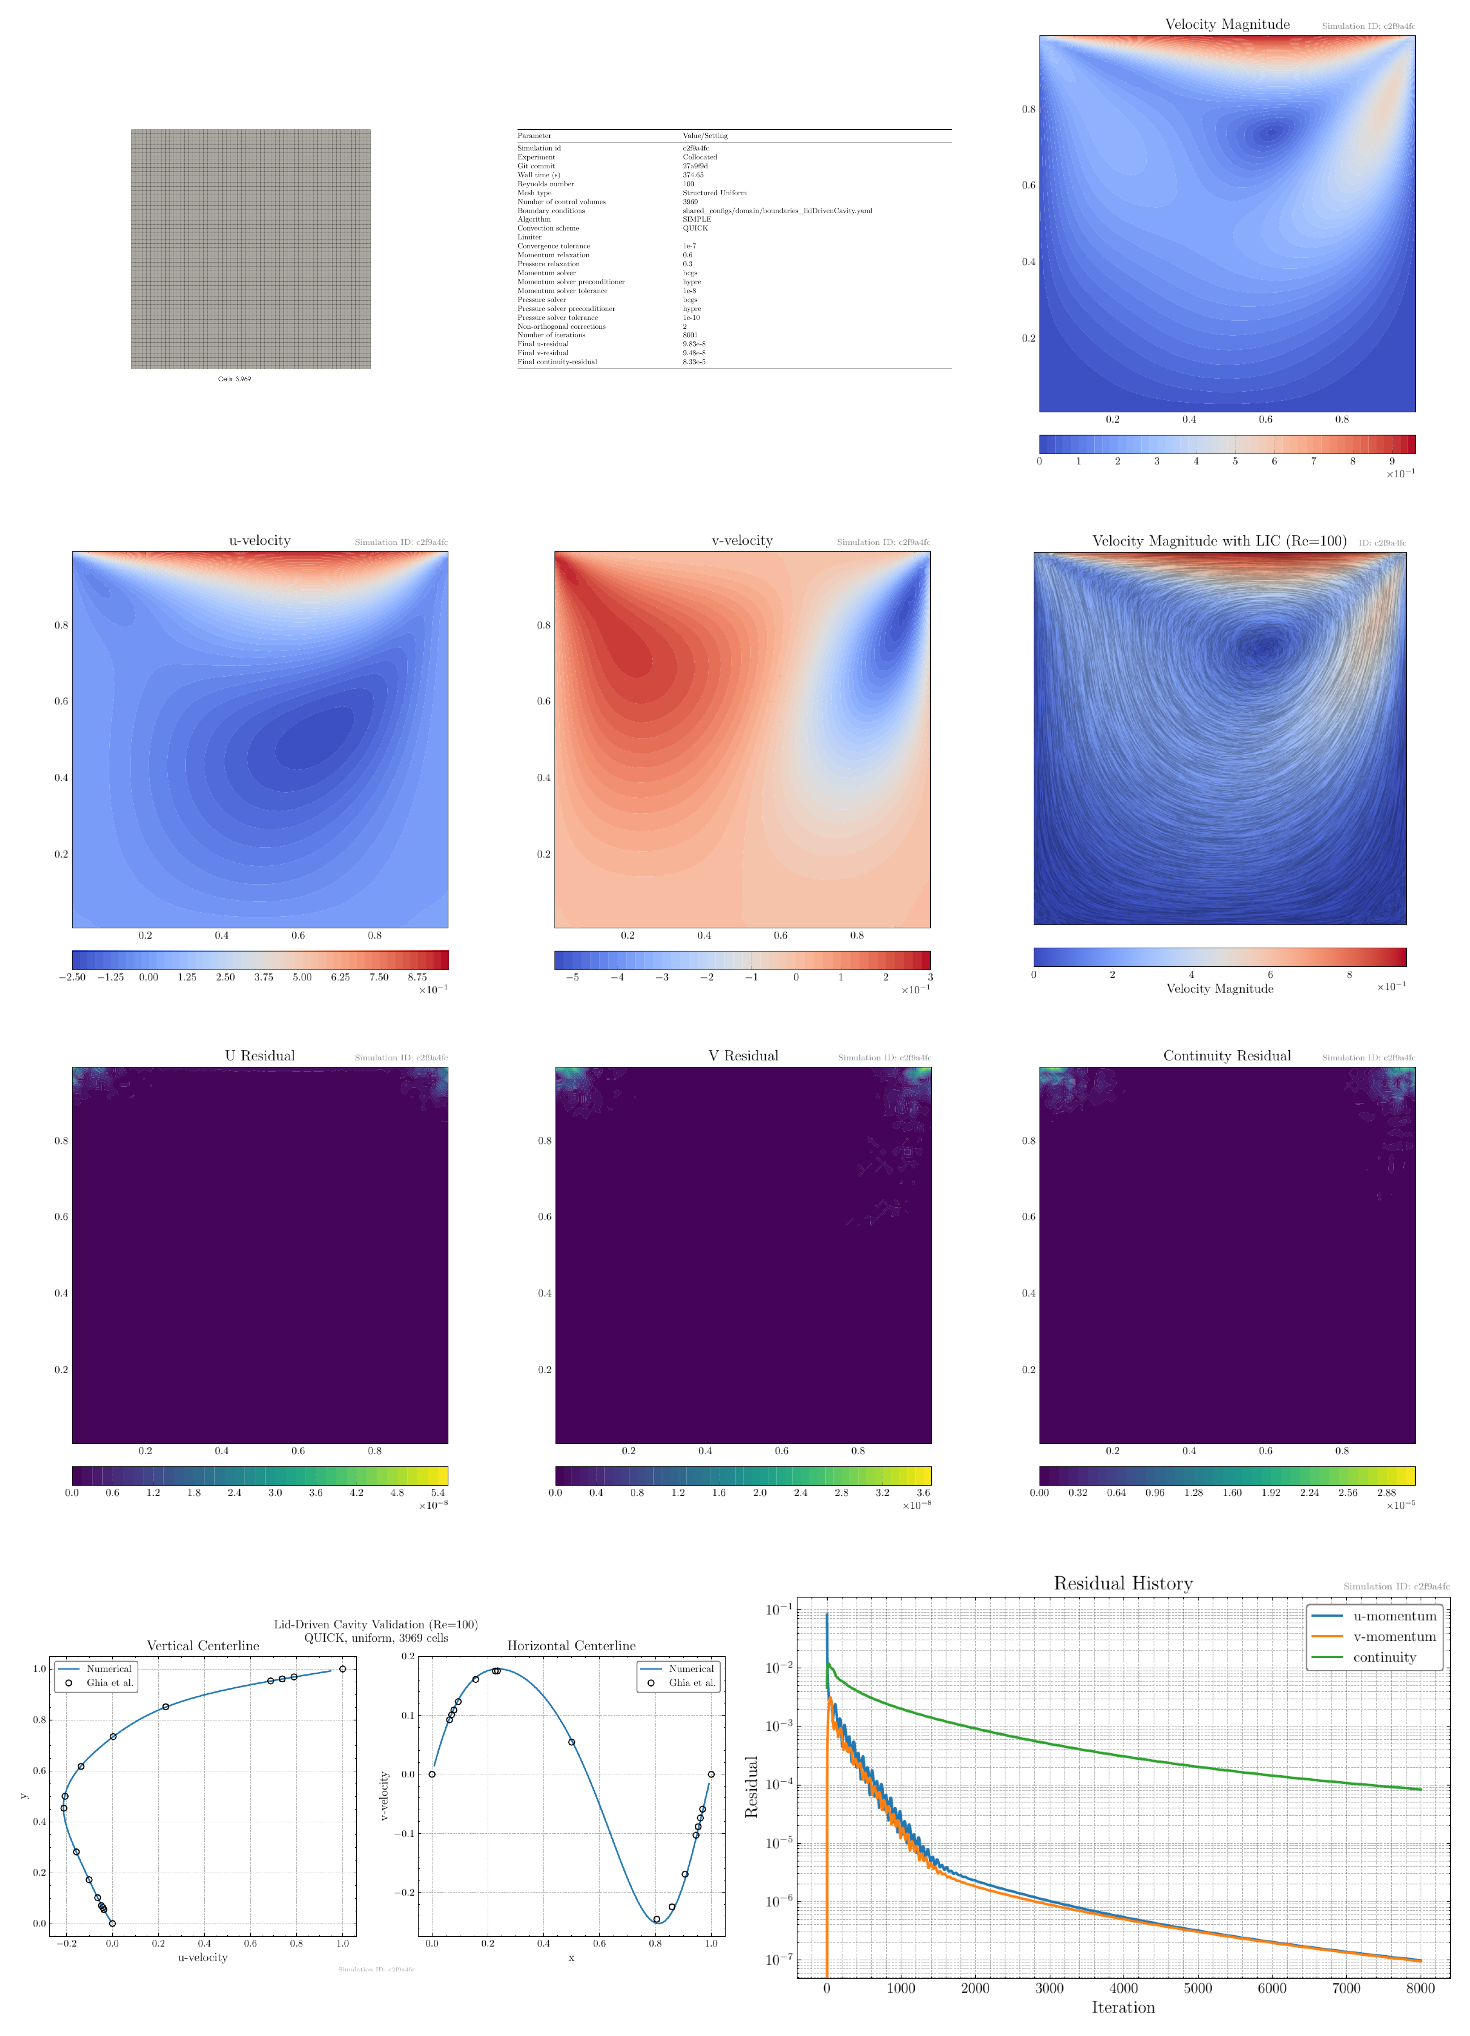
\includegraphics[width=0.85\linewidth]{AppendixPlots/lidDrivenCavity/Re_100/coarse/lidDrivenCavity_Re100_uniform_coarse_QUICK_c2f9a4fc.pdf}
    \caption{Liddrivencavity simulation at Re=100 using uniform coarse mesh with QUICK discretization scheme (Simulation ID: c2f9a4fc)}
    \label{sim.ldc.re100.unif.coarse.quick}
\end{figure}

\paragraph*{Uniform Mesh with TVD Scheme}
\addcontentsline{toc}{paragraph}{Uniform Mesh with TVD Scheme}
\label{para:liddrivencavity_re100_coarse_uniform_TVD}

\begin{figure}[H]
    \centering
    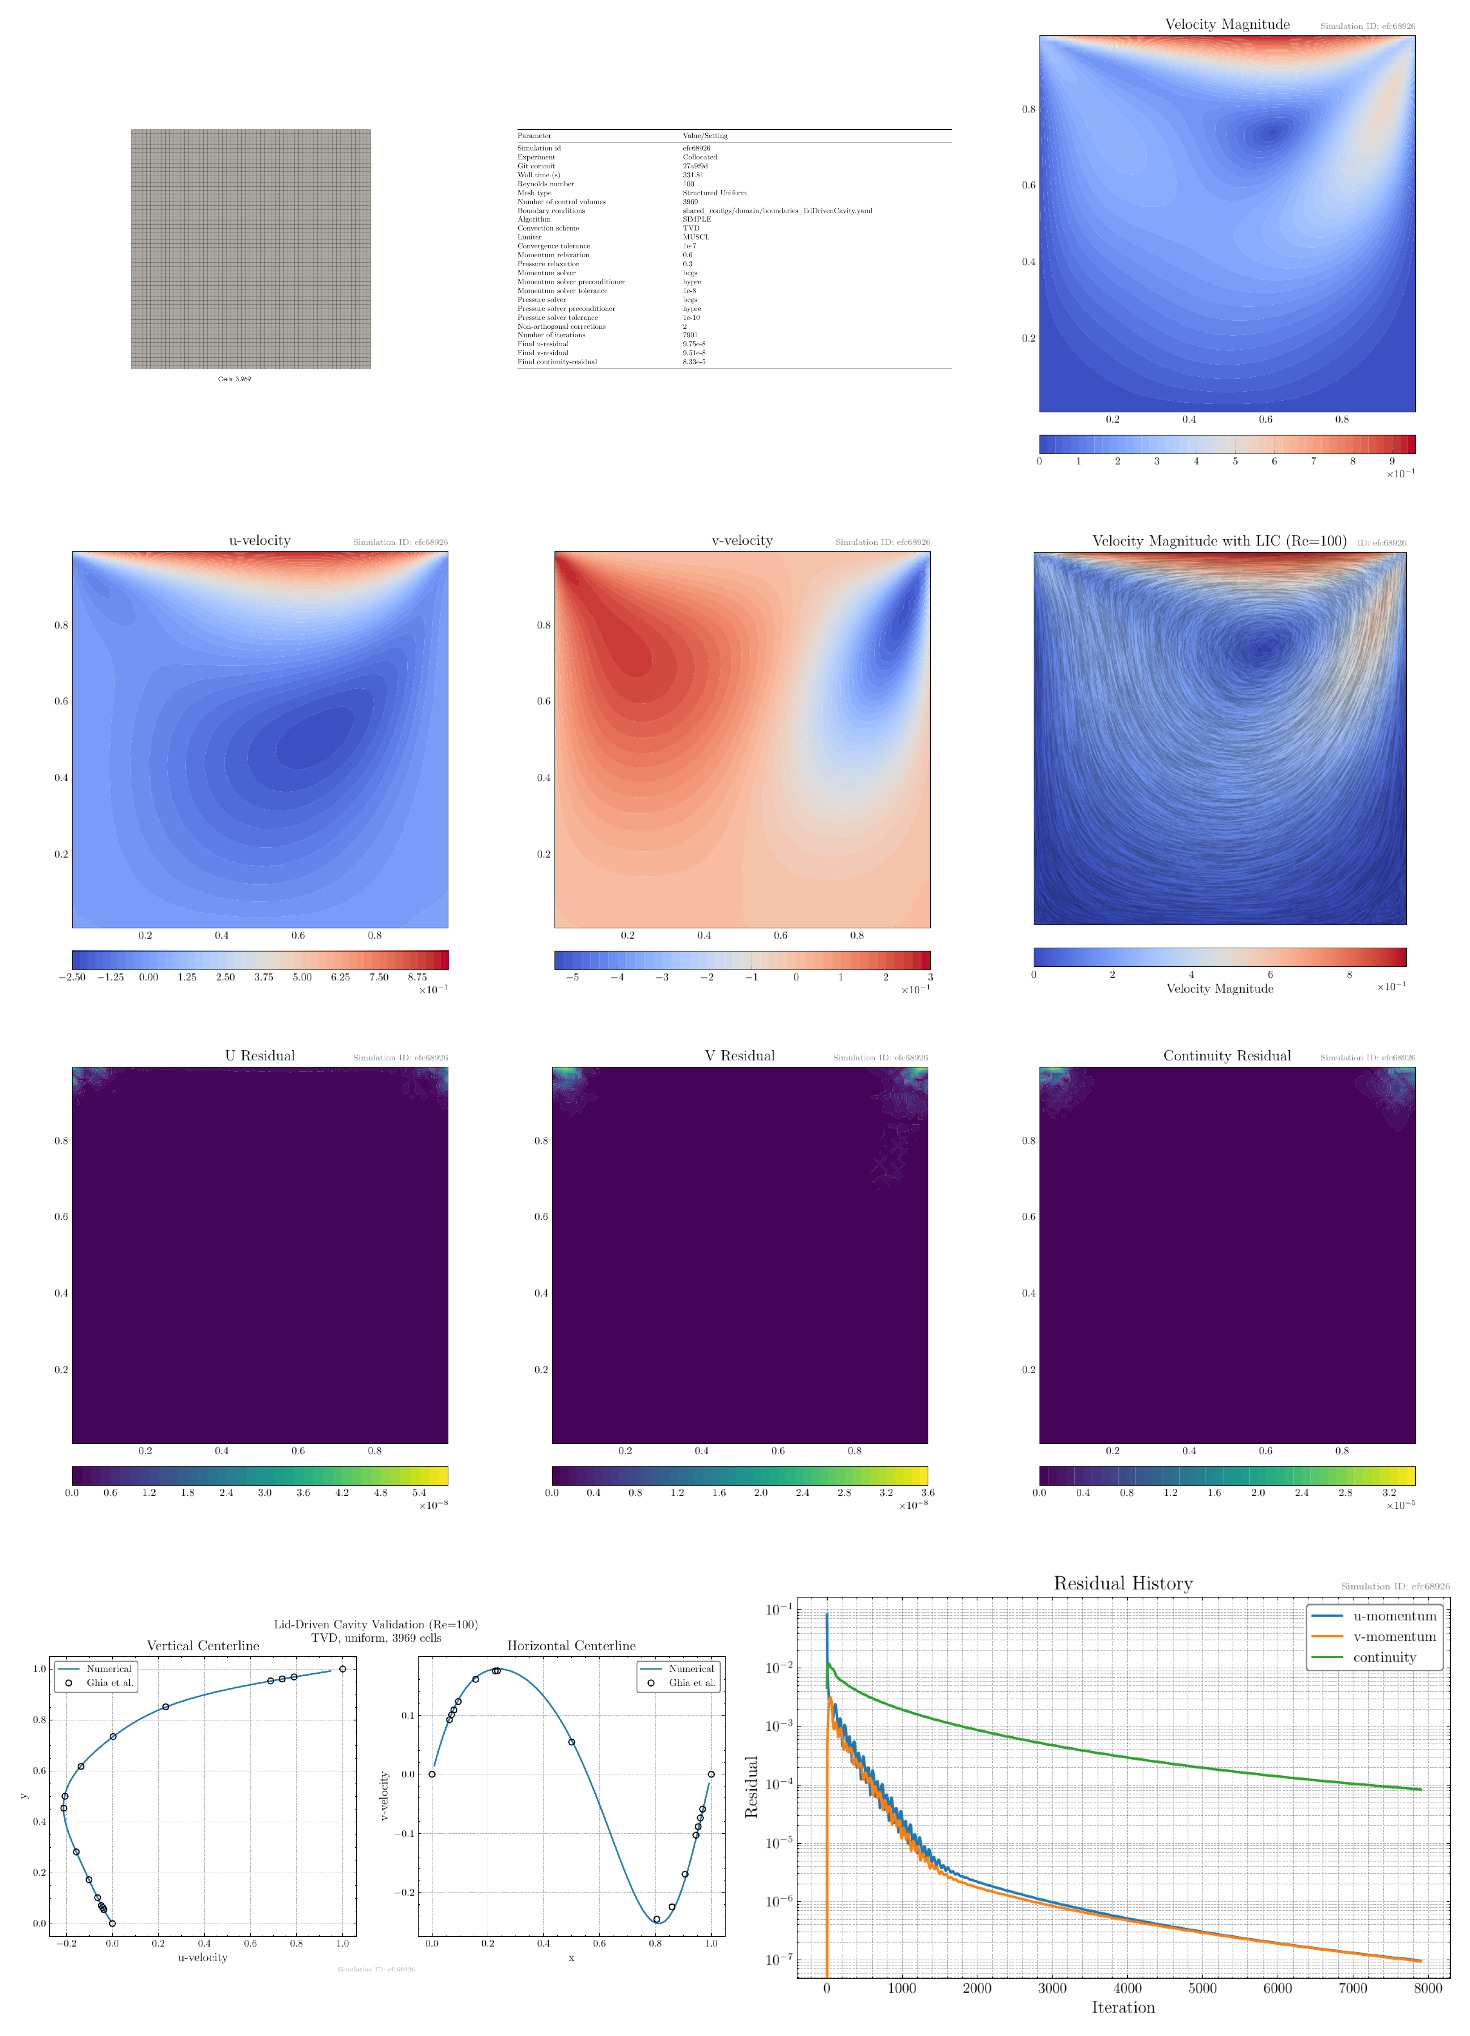
\includegraphics[width=0.85\linewidth]{AppendixPlots/lidDrivenCavity/Re_100/coarse/lidDrivenCavity_Re100_uniform_coarse_TVD_efc68926.pdf}
    \caption{Liddrivencavity simulation at Re=100 using uniform coarse mesh with TVD discretization scheme (Simulation ID: efc68926)}
    \label{sim.ldc.re100.unif.coarse.tvd}
\end{figure}

\paragraph*{Uniform Mesh with Upwind Scheme}
\addcontentsline{toc}{paragraph}{Uniform Mesh with Upwind Scheme}
\label{para:liddrivencavity_re100_coarse_uniform_Upwind}

\begin{figure}[H]
    \centering
    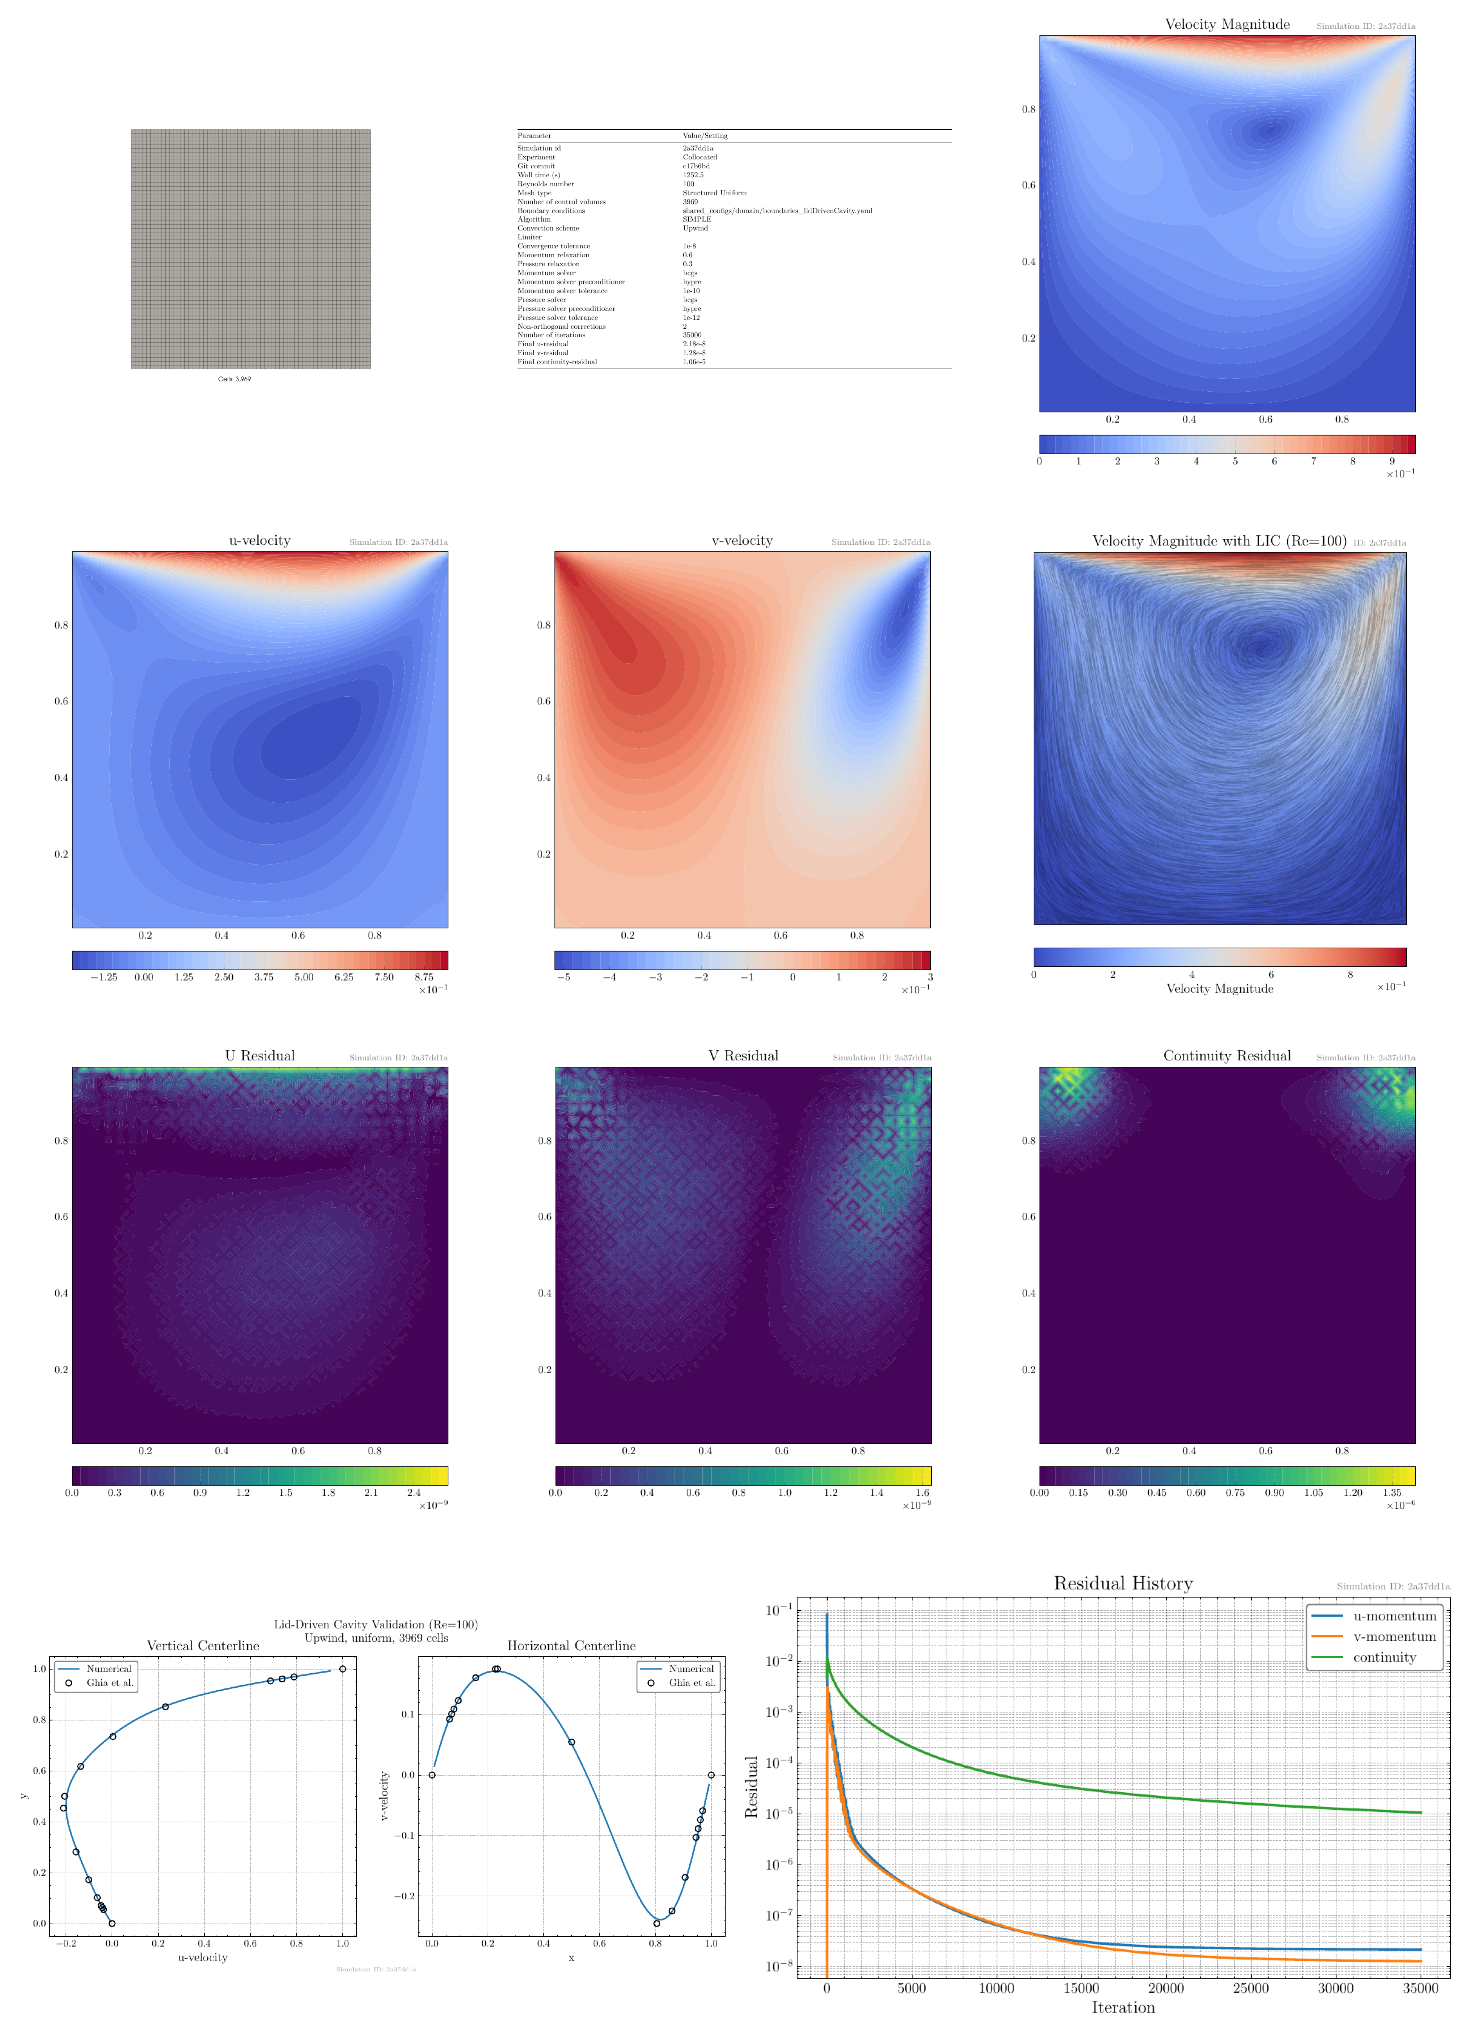
\includegraphics[width=0.85\linewidth]{AppendixPlots/lidDrivenCavity/Re_100/coarse/lidDrivenCavity_Re100_uniform_coarse_Upwind_2a37dd1a.pdf}
    \caption{Liddrivencavity simulation at Re=100 using uniform coarse mesh with Upwind discretization scheme (Simulation ID: 2a37dd1a)}
    \label{sim.ldc.re100.unif.coarse.upwind}
\end{figure}

\paragraph*{Unstructured Mesh with QUICK Scheme}
\addcontentsline{toc}{paragraph}{Unstructured Mesh with QUICK Scheme}
\label{para:liddrivencavity_re100_coarse_unstructured_QUICK}

\begin{figure}[H]
    \centering
    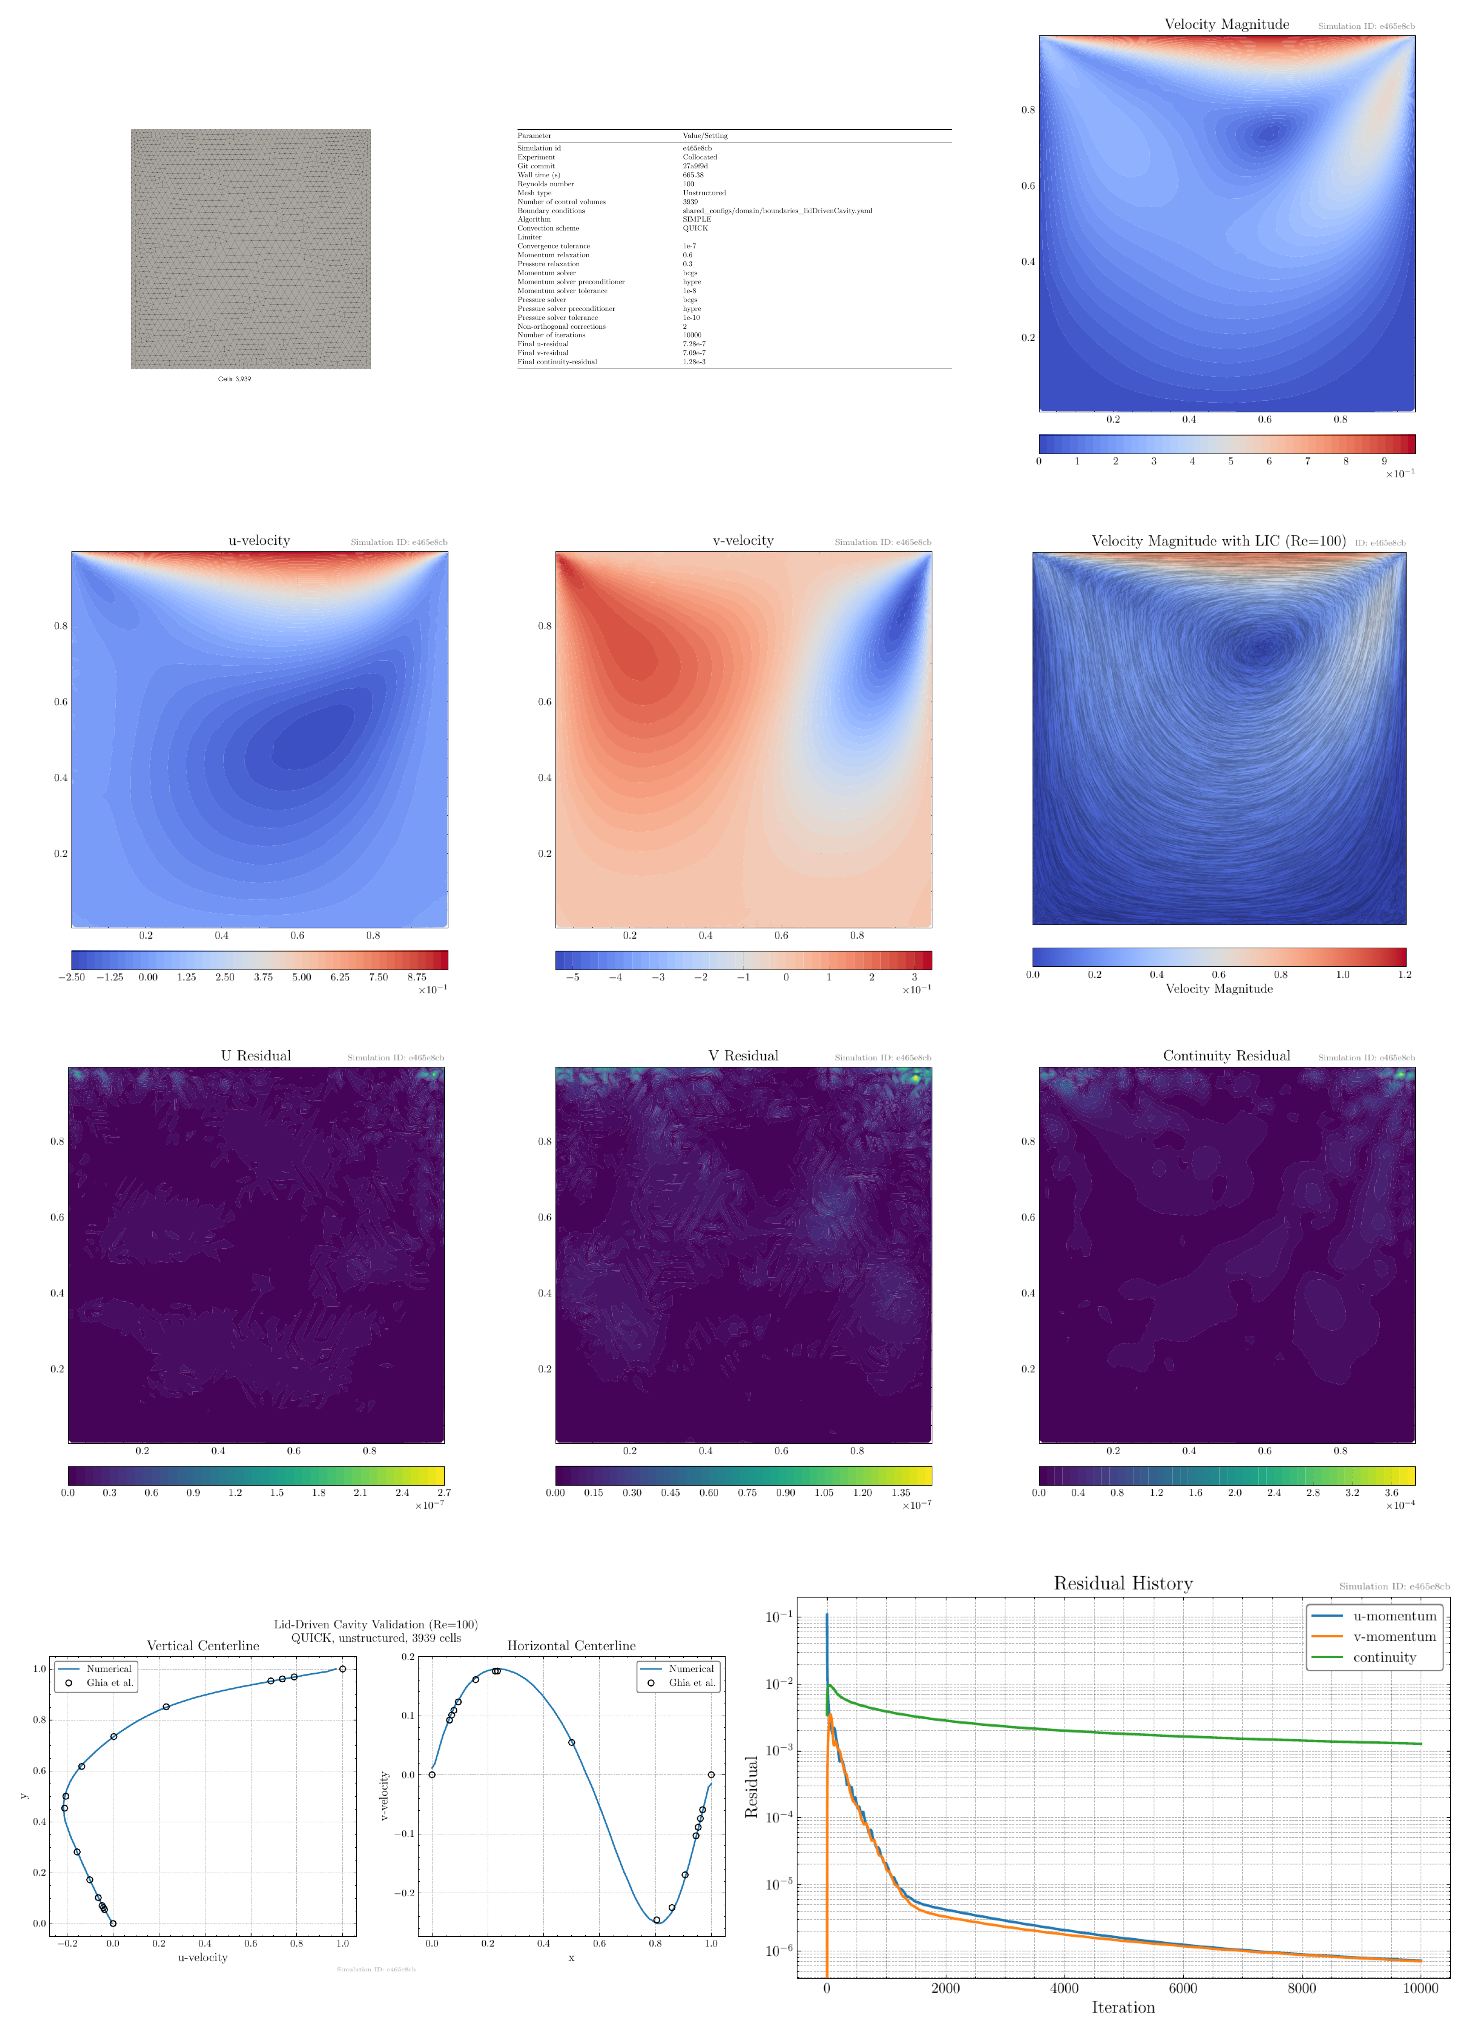
\includegraphics[width=0.85\linewidth]{AppendixPlots/lidDrivenCavity/Re_100/coarse/lidDrivenCavity_Re100_unstructured_coarse_QUICK_e465e8cb.pdf}
    \caption{Liddrivencavity simulation at Re=100 using unstructured coarse mesh with QUICK discretization scheme (Simulation ID: e465e8cb)}
    \label{sim.ldc.re100.unstruct.coarse.quick}
\end{figure}

\paragraph*{Unstructured Mesh with TVD Scheme}
\addcontentsline{toc}{paragraph}{Unstructured Mesh with TVD Scheme}
\label{para:liddrivencavity_re100_coarse_unstructured_TVD}

\begin{figure}[H]
    \centering
    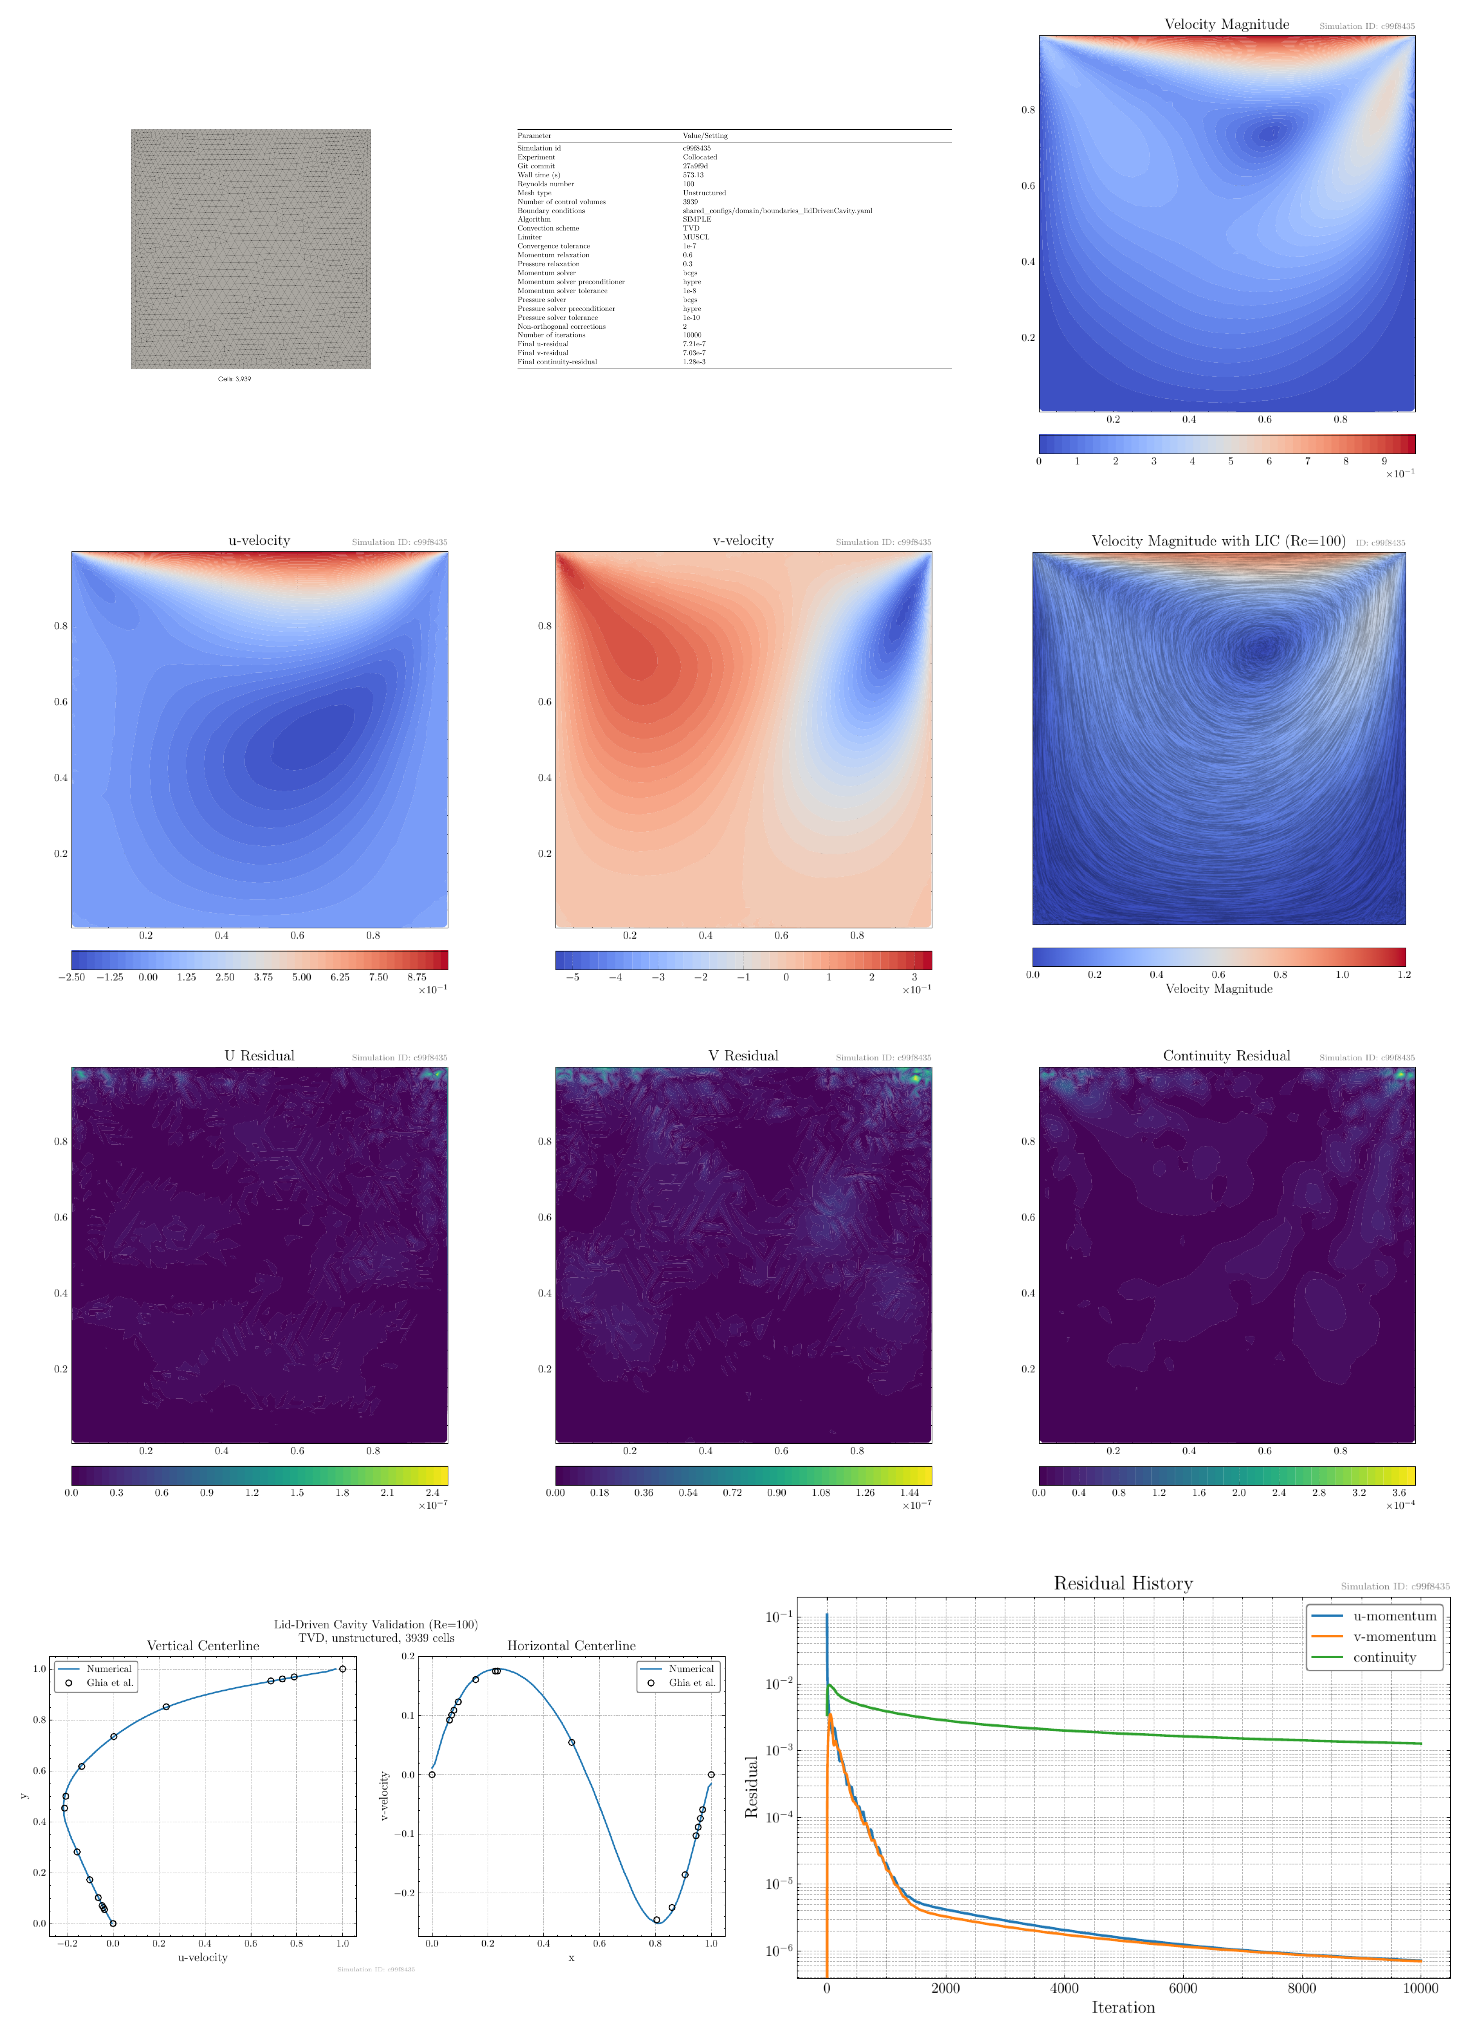
\includegraphics[width=0.85\linewidth]{AppendixPlots/lidDrivenCavity/Re_100/coarse/lidDrivenCavity_Re100_unstructured_coarse_TVD_c99f8435.pdf}
    \caption{Liddrivencavity simulation at Re=100 using unstructured coarse mesh with TVD discretization scheme (Simulation ID: c99f8435)}
    \label{sim.ldc.re100.unstruct.coarse.tvd}
\end{figure}

\paragraph*{Unstructured Mesh with Upwind Scheme}
\addcontentsline{toc}{paragraph}{Unstructured Mesh with Upwind Scheme}
\label{para:liddrivencavity_re100_coarse_unstructured_Upwind}

\begin{figure}[H]
    \centering
    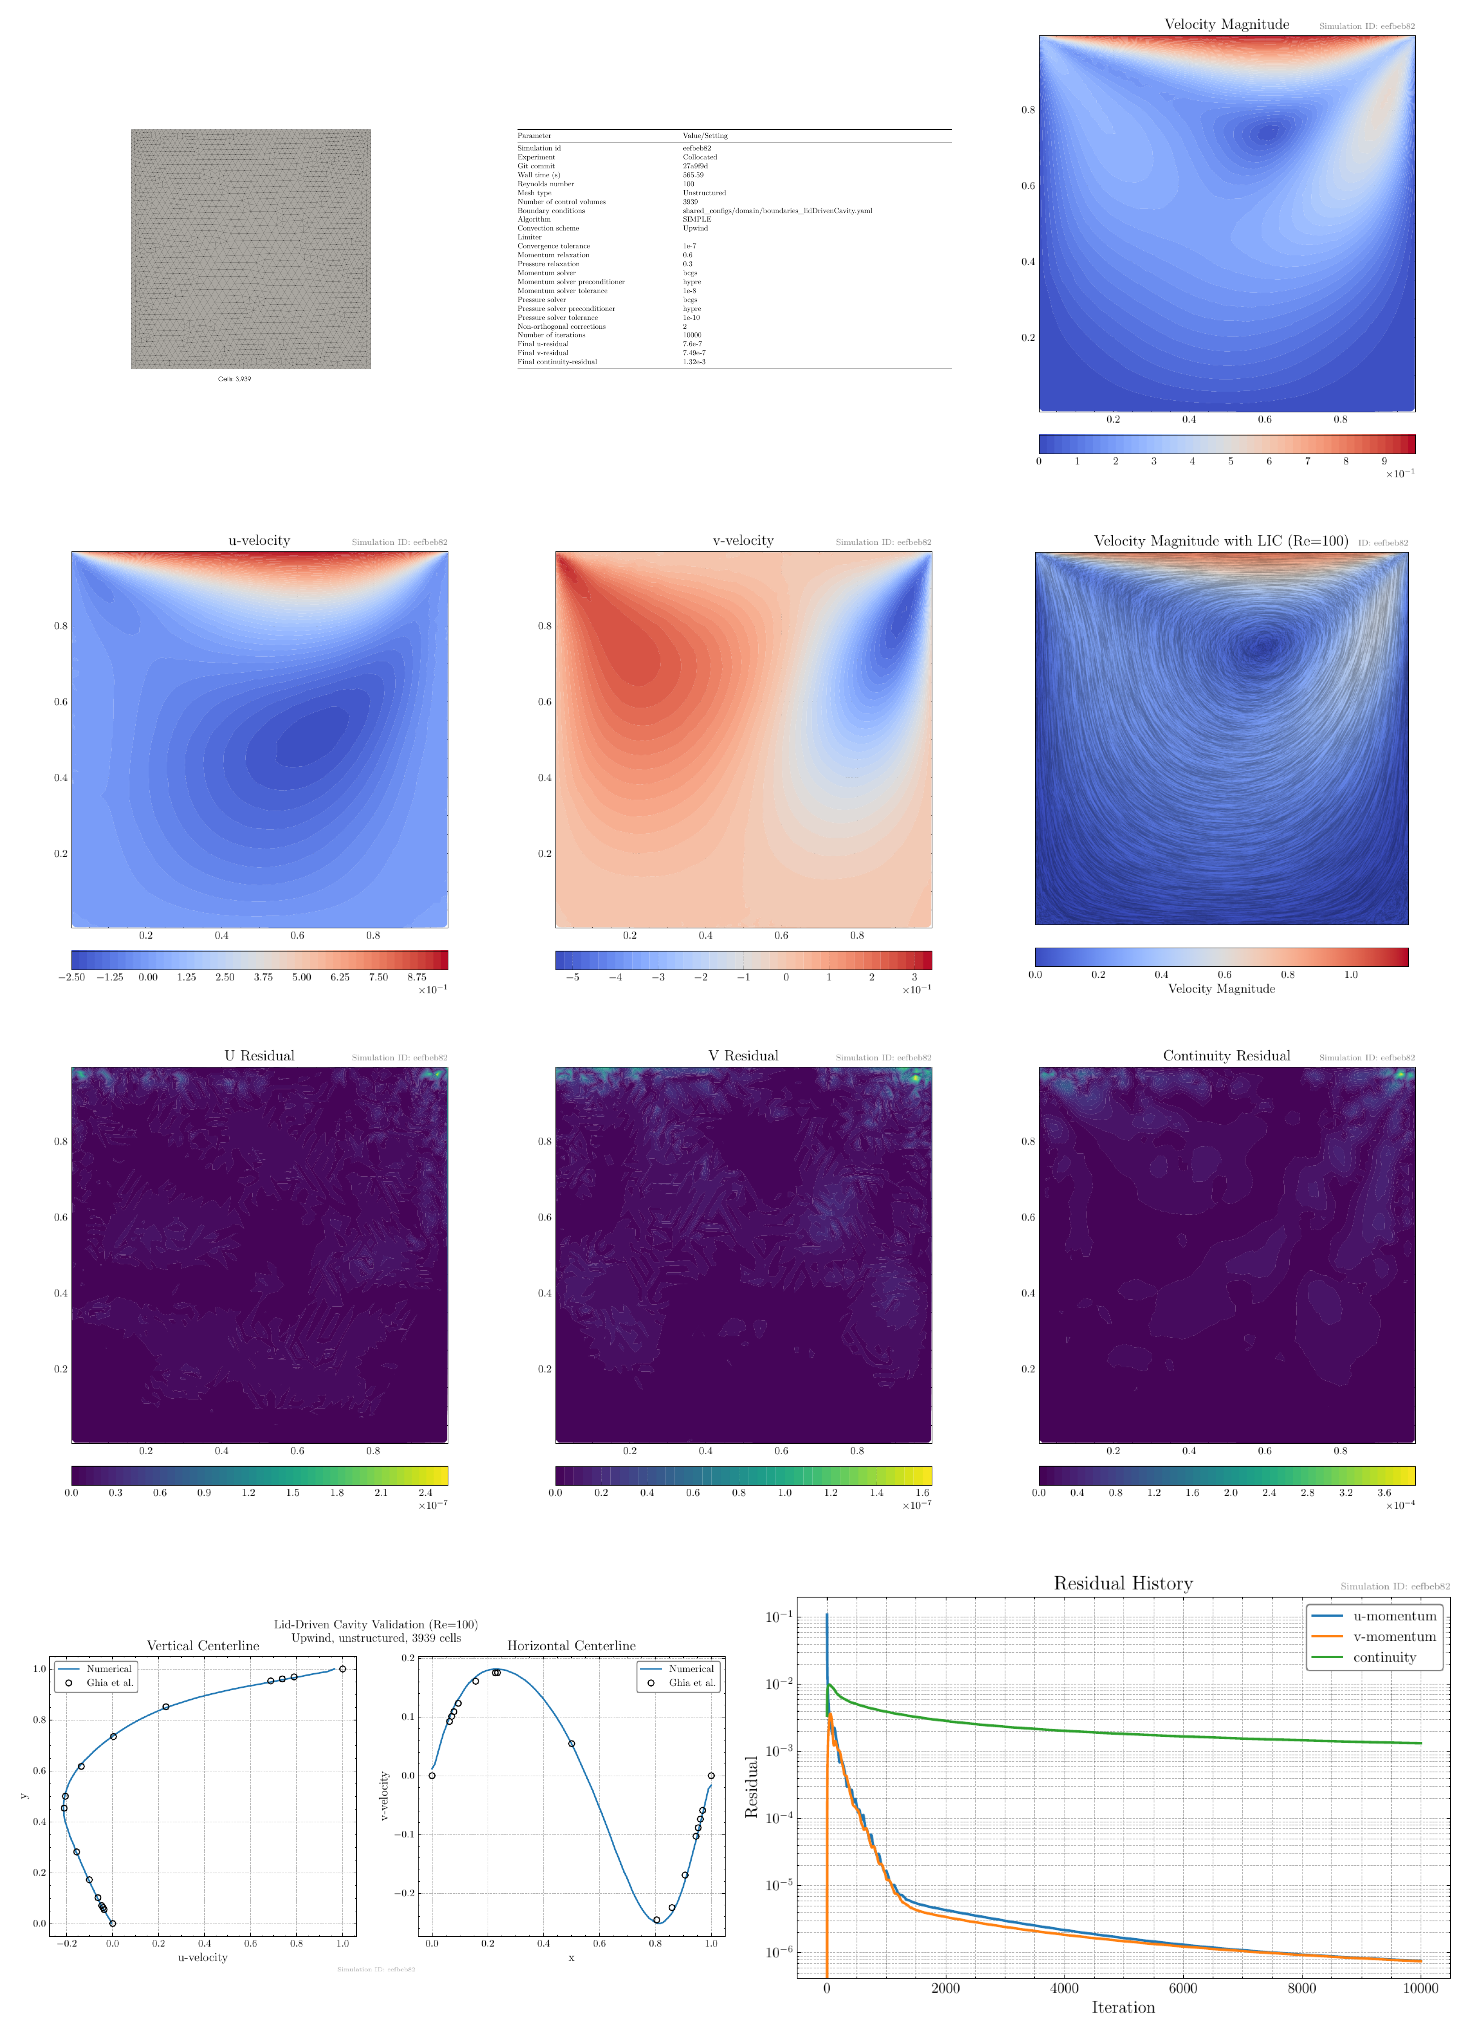
\includegraphics[width=0.85\linewidth]{AppendixPlots/lidDrivenCavity/Re_100/coarse/lidDrivenCavity_Re100_unstructured_coarse_Upwind_eefbeb82.pdf}
    \caption{Liddrivencavity simulation at Re=100 using unstructured coarse mesh with Upwind discretization scheme (Simulation ID: eefbeb82)}
    \label{sim.ldc.re100.unstruct.coarse.upwind}
\end{figure}

\clearpage

\subsubsection*{Medium Mesh}
\addcontentsline{toc}{subsubsection}{Medium Mesh}
\label{subsubsec:liddrivencavity_re100_medium}

\paragraph*{Uniform Mesh with QUICK Scheme}
\addcontentsline{toc}{paragraph}{Uniform Mesh with QUICK Scheme}
\label{para:liddrivencavity_re100_medium_uniform_QUICK}

\begin{figure}[H]
    \centering
    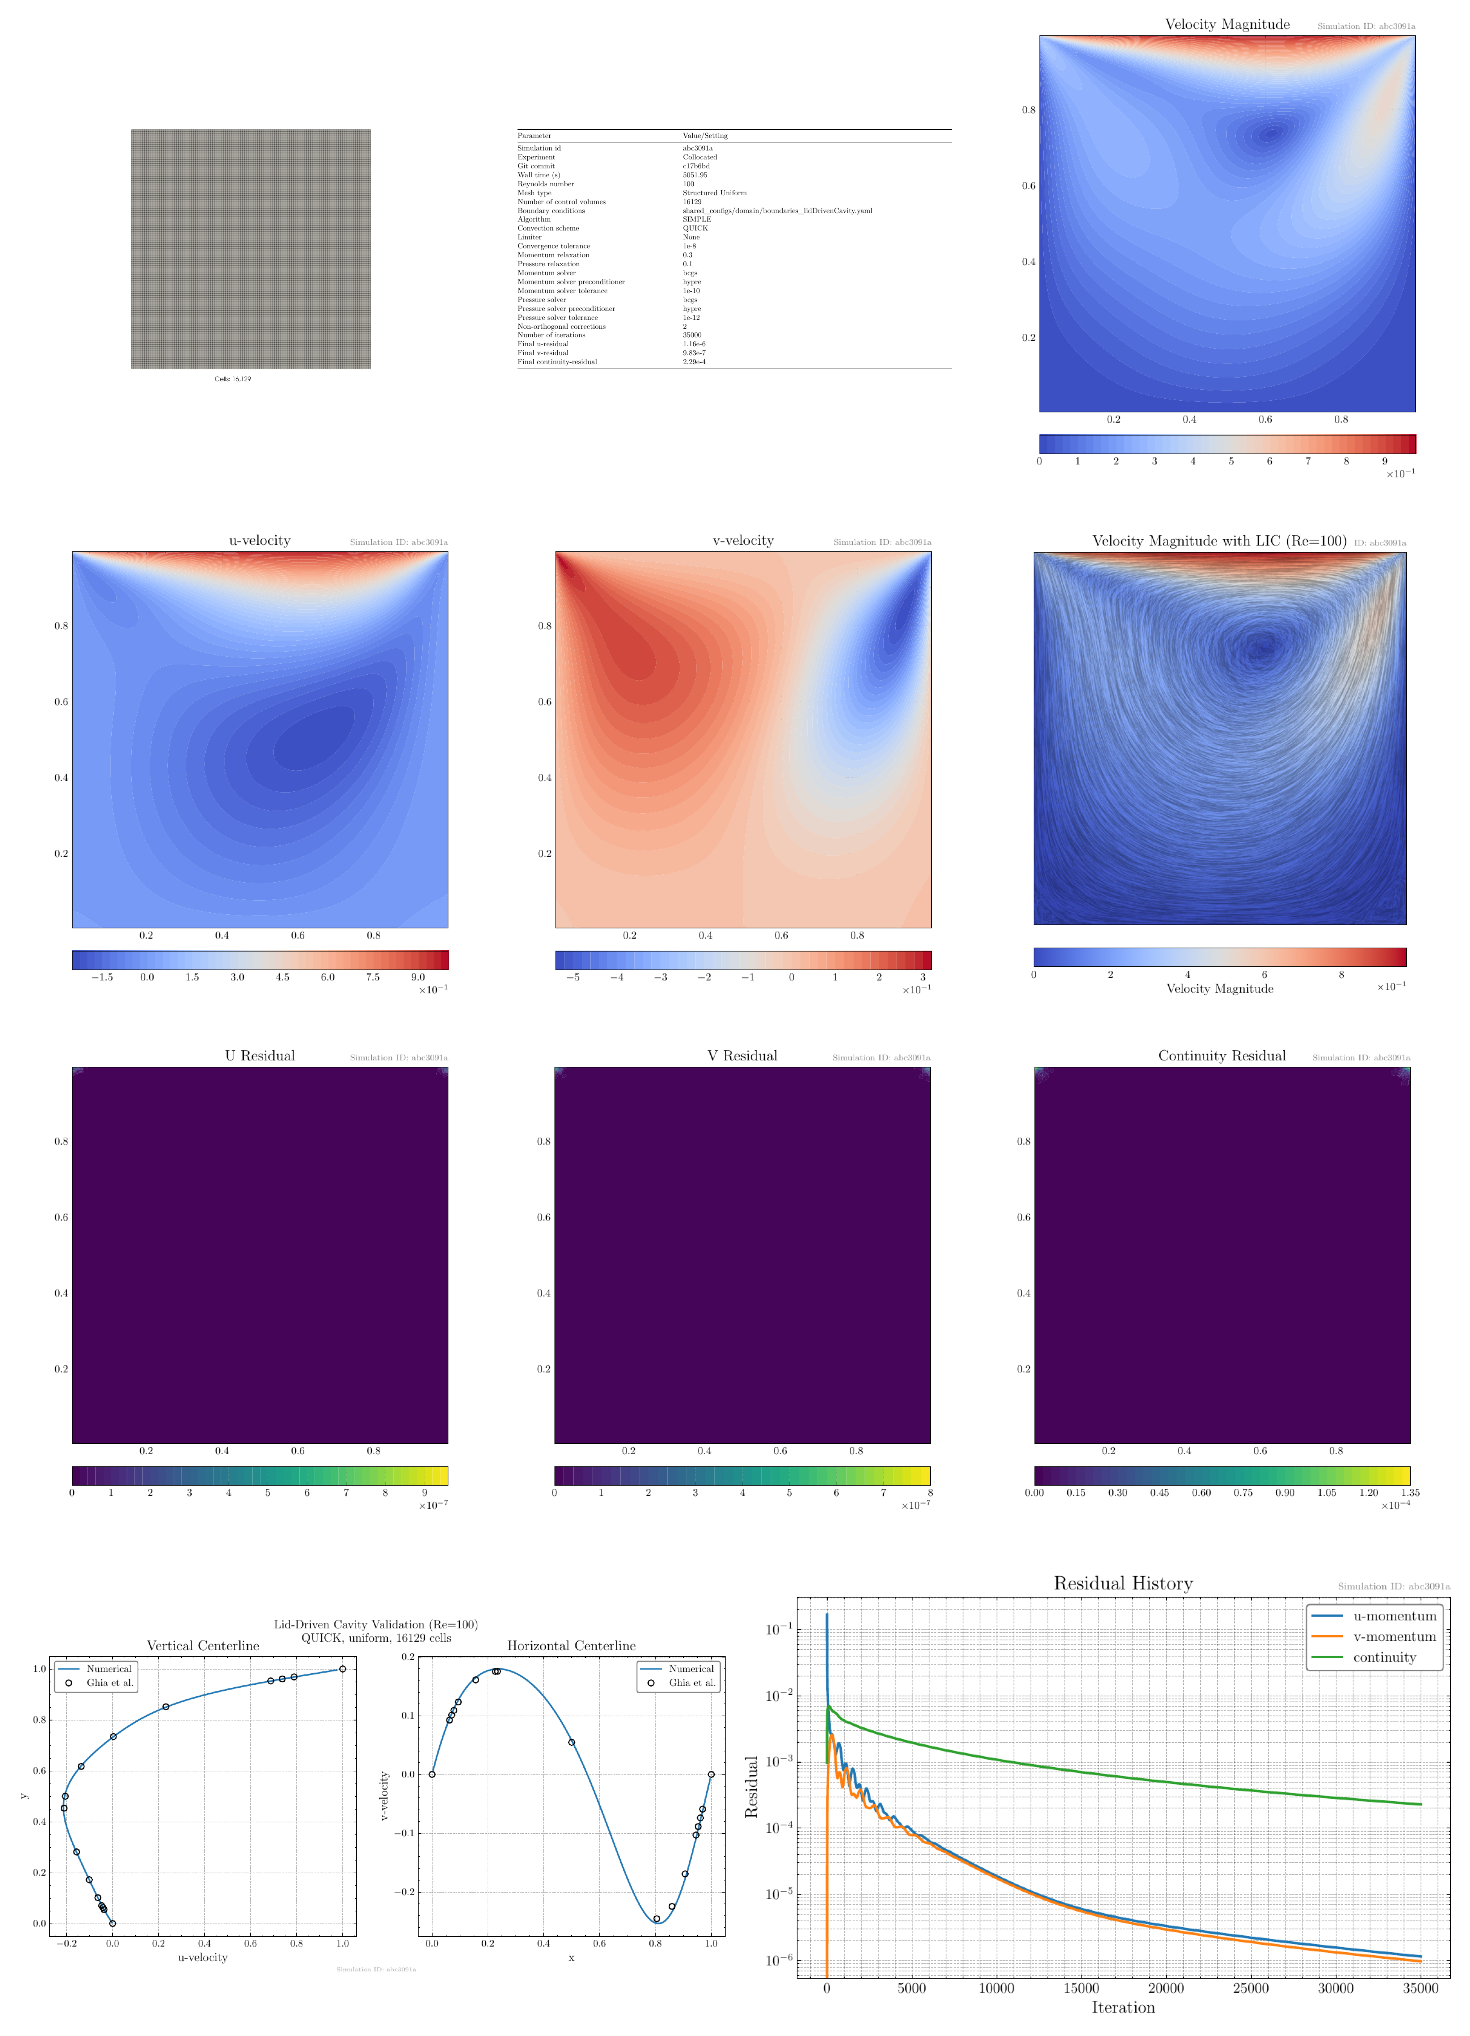
\includegraphics[width=0.85\linewidth]{AppendixPlots/lidDrivenCavity/Re_100/medium/lidDrivenCavity_Re100_uniform_medium_QUICK_abc3091a.pdf}
    \caption{Liddrivencavity simulation at Re=100 using uniform medium mesh with QUICK discretization scheme (Simulation ID: abc3091a)}
    \label{sim.ldc.re100.unif.med.quick}
\end{figure}

\paragraph*{Uniform Mesh with TVD Scheme}
\addcontentsline{toc}{paragraph}{Uniform Mesh with TVD Scheme}
\label{para:liddrivencavity_re100_medium_uniform_TVD}

\begin{figure}[H]
    \centering
    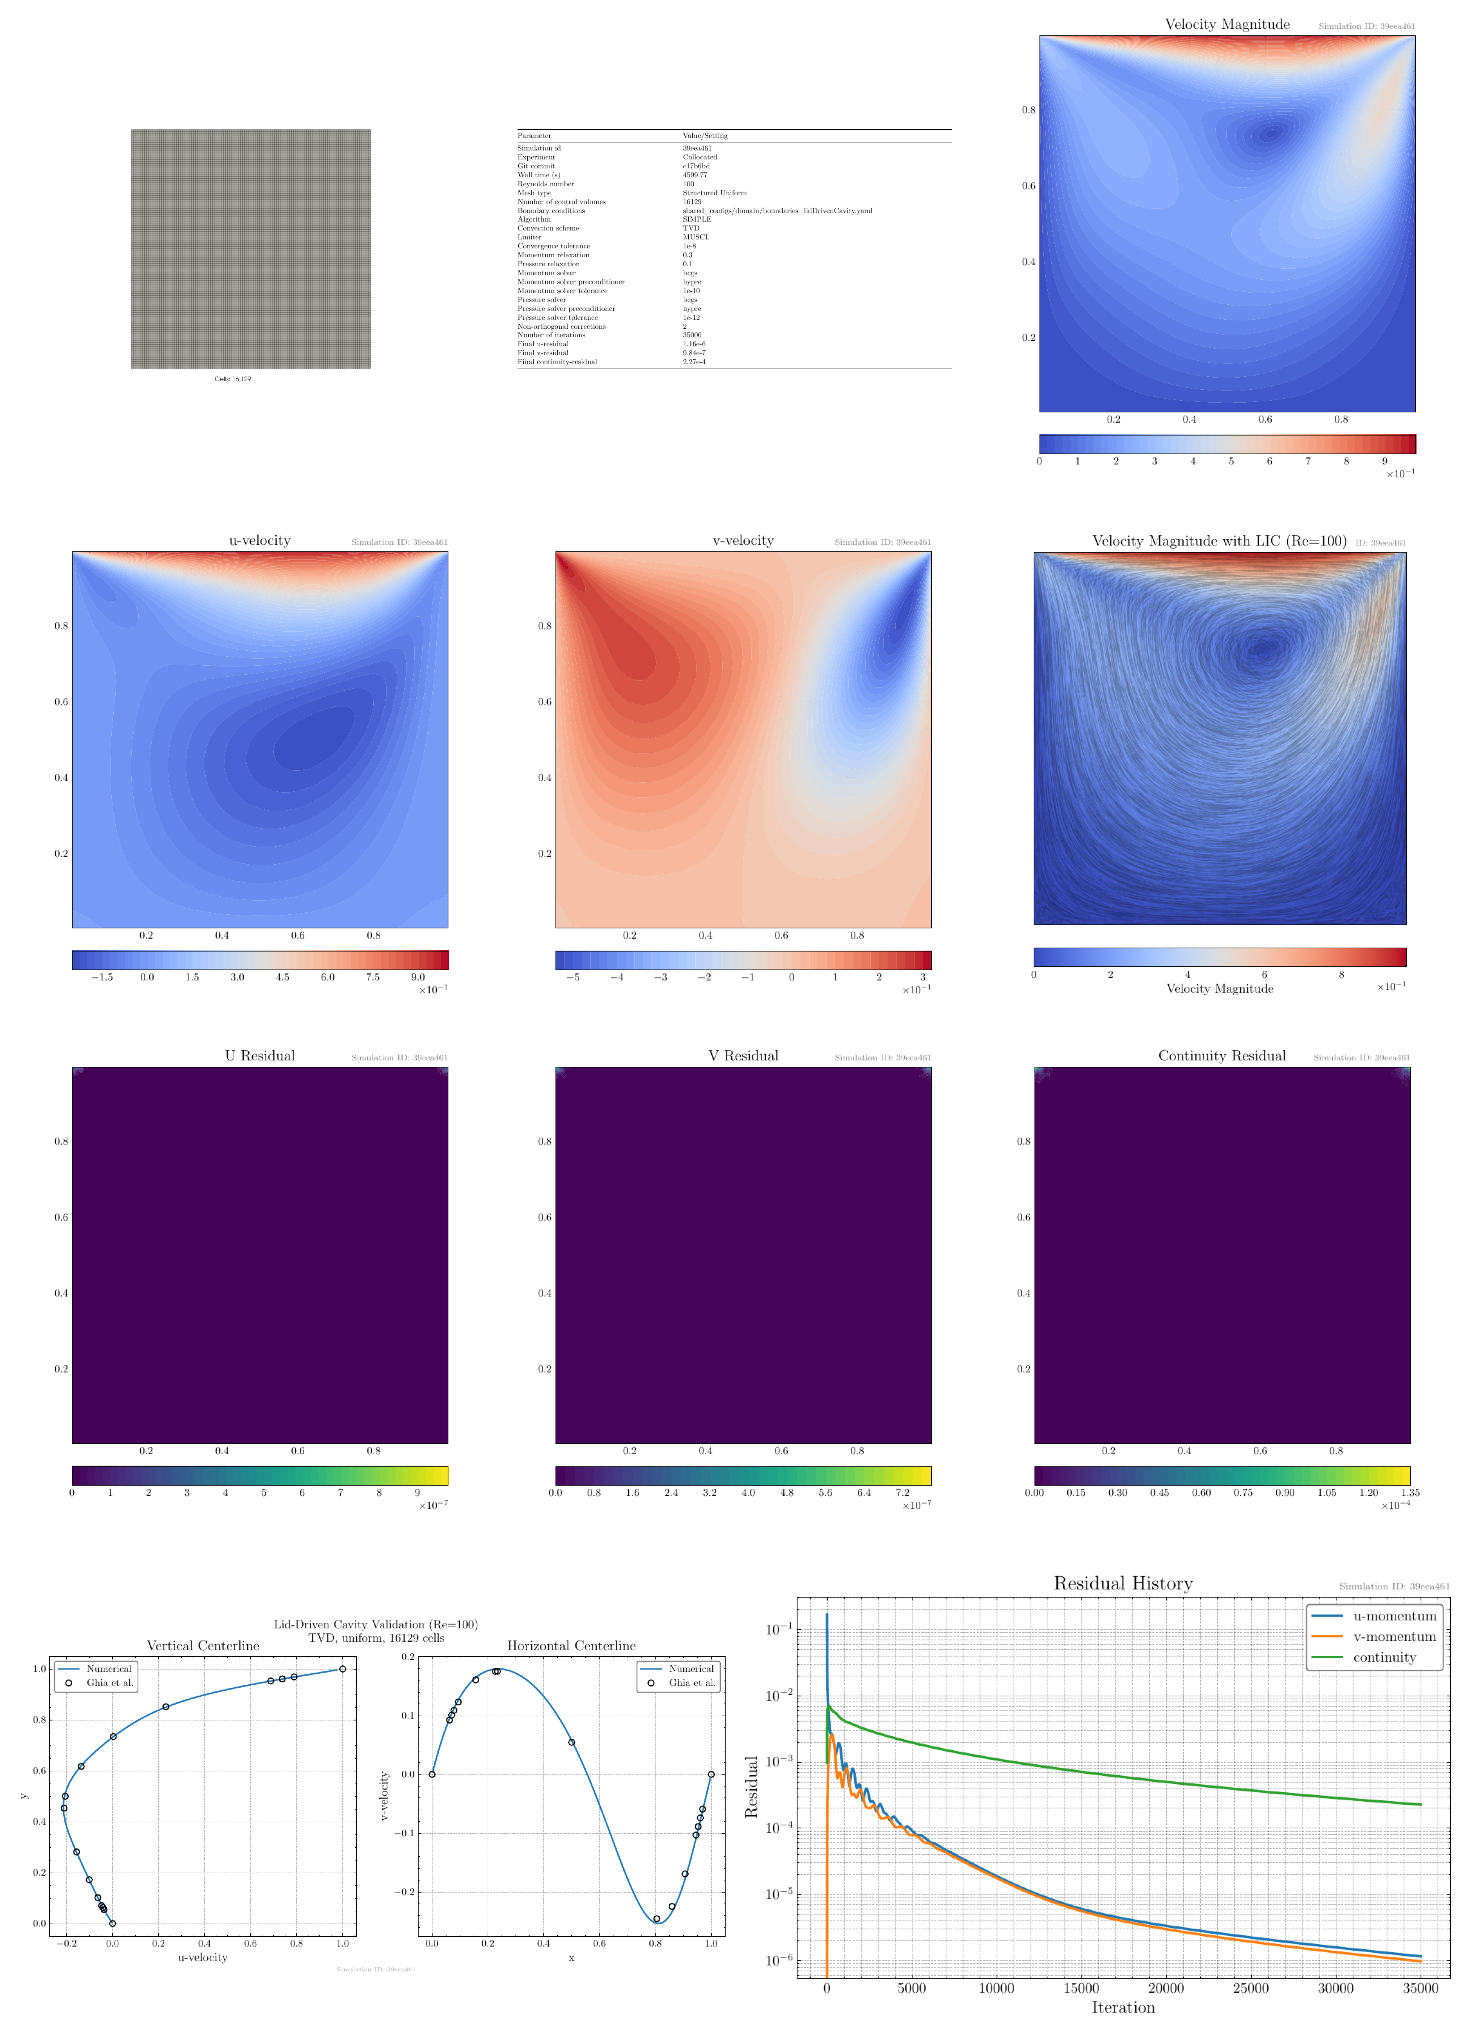
\includegraphics[width=0.85\linewidth]{AppendixPlots/lidDrivenCavity/Re_100/medium/lidDrivenCavity_Re100_uniform_medium_TVD_39eea461.pdf}
    \caption{Liddrivencavity simulation at Re=100 using uniform medium mesh with TVD discretization scheme (Simulation ID: 39eea461)}
    \label{sim.ldc.re100.unif.med.tvd}
\end{figure}

\paragraph*{Uniform Mesh with Upwind Scheme}
\addcontentsline{toc}{paragraph}{Uniform Mesh with Upwind Scheme}
\label{para:liddrivencavity_re100_medium_uniform_Upwind}

\begin{figure}[H]
    \centering
    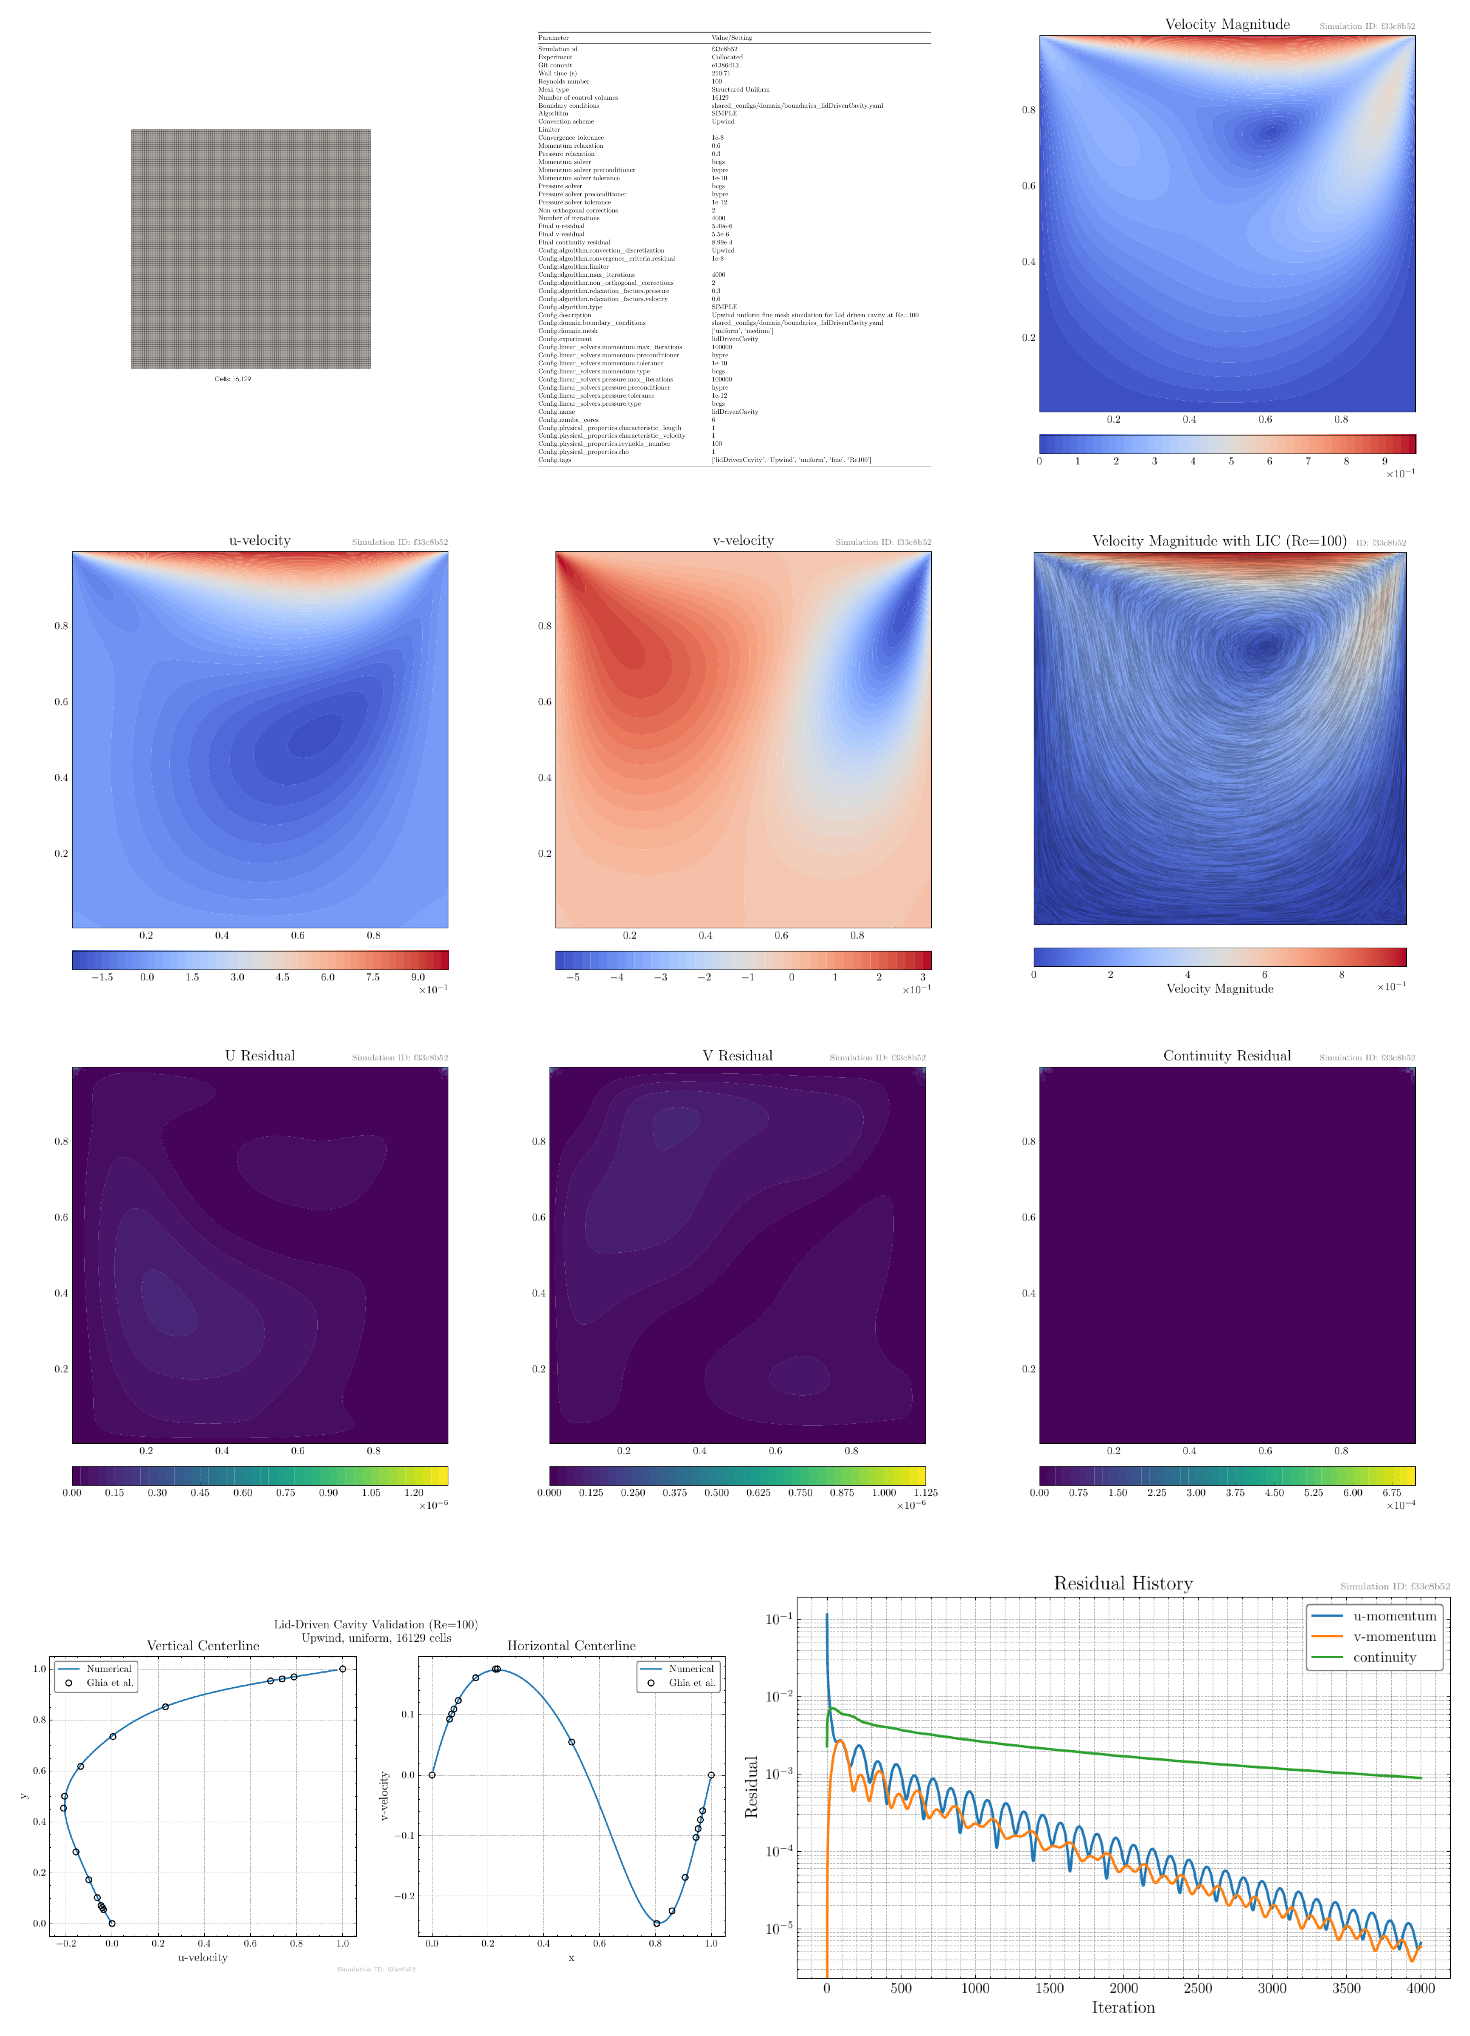
\includegraphics[width=0.85\linewidth]{AppendixPlots/lidDrivenCavity/Re_100/medium/lidDrivenCavity_Re100_uniform_medium_Upwind_f33c8b52.pdf}
    \caption{Liddrivencavity simulation at Re=100 using uniform medium mesh with Upwind discretization scheme (Simulation ID: f33c8b52)}
    \label{sim.ldc.re100.unif.med.upwind}
\end{figure}

\begin{figure}[H]
    \centering
    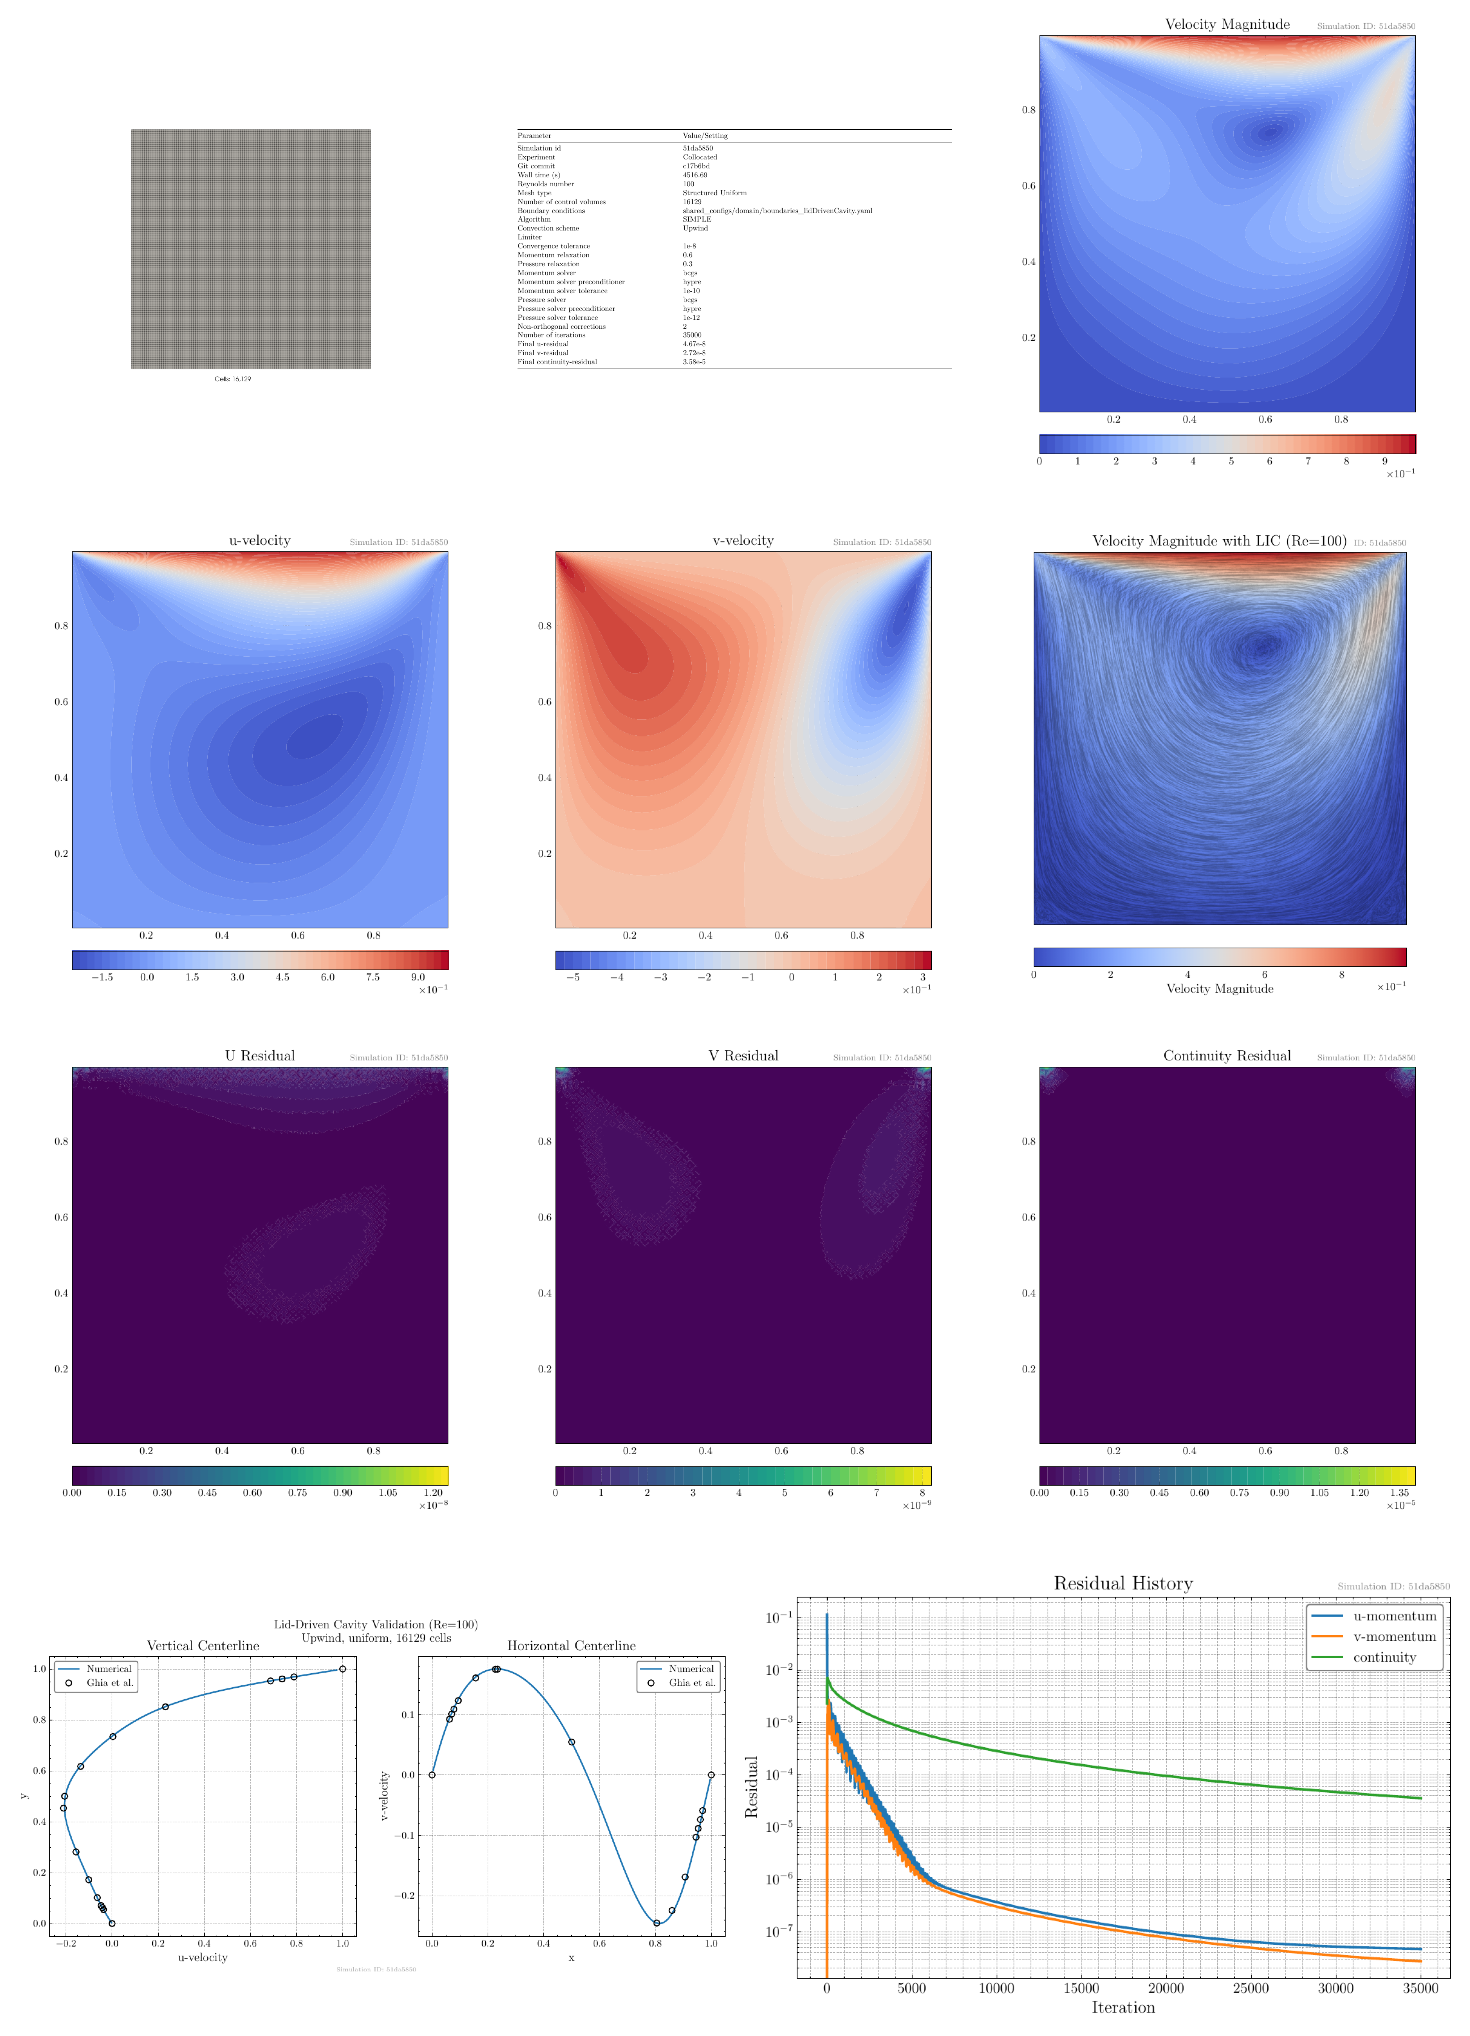
\includegraphics[width=0.85\linewidth]{AppendixPlots/lidDrivenCavity/Re_100/medium/lidDrivenCavity_Re100_uniform_medium_Upwind_51da5850.pdf}
    \caption{Liddrivencavity simulation at Re=100 using uniform medium mesh with Upwind discretization scheme (Simulation ID: 51da5850)}
    \label{sim.ldc.re100.unif.med.upwind}
\end{figure}

\paragraph*{Unstructured Mesh with QUICK Scheme}
\addcontentsline{toc}{paragraph}{Unstructured Mesh with QUICK Scheme}
\label{para:liddrivencavity_re100_medium_unstructured_QUICK}

\begin{figure}[H]
    \centering
    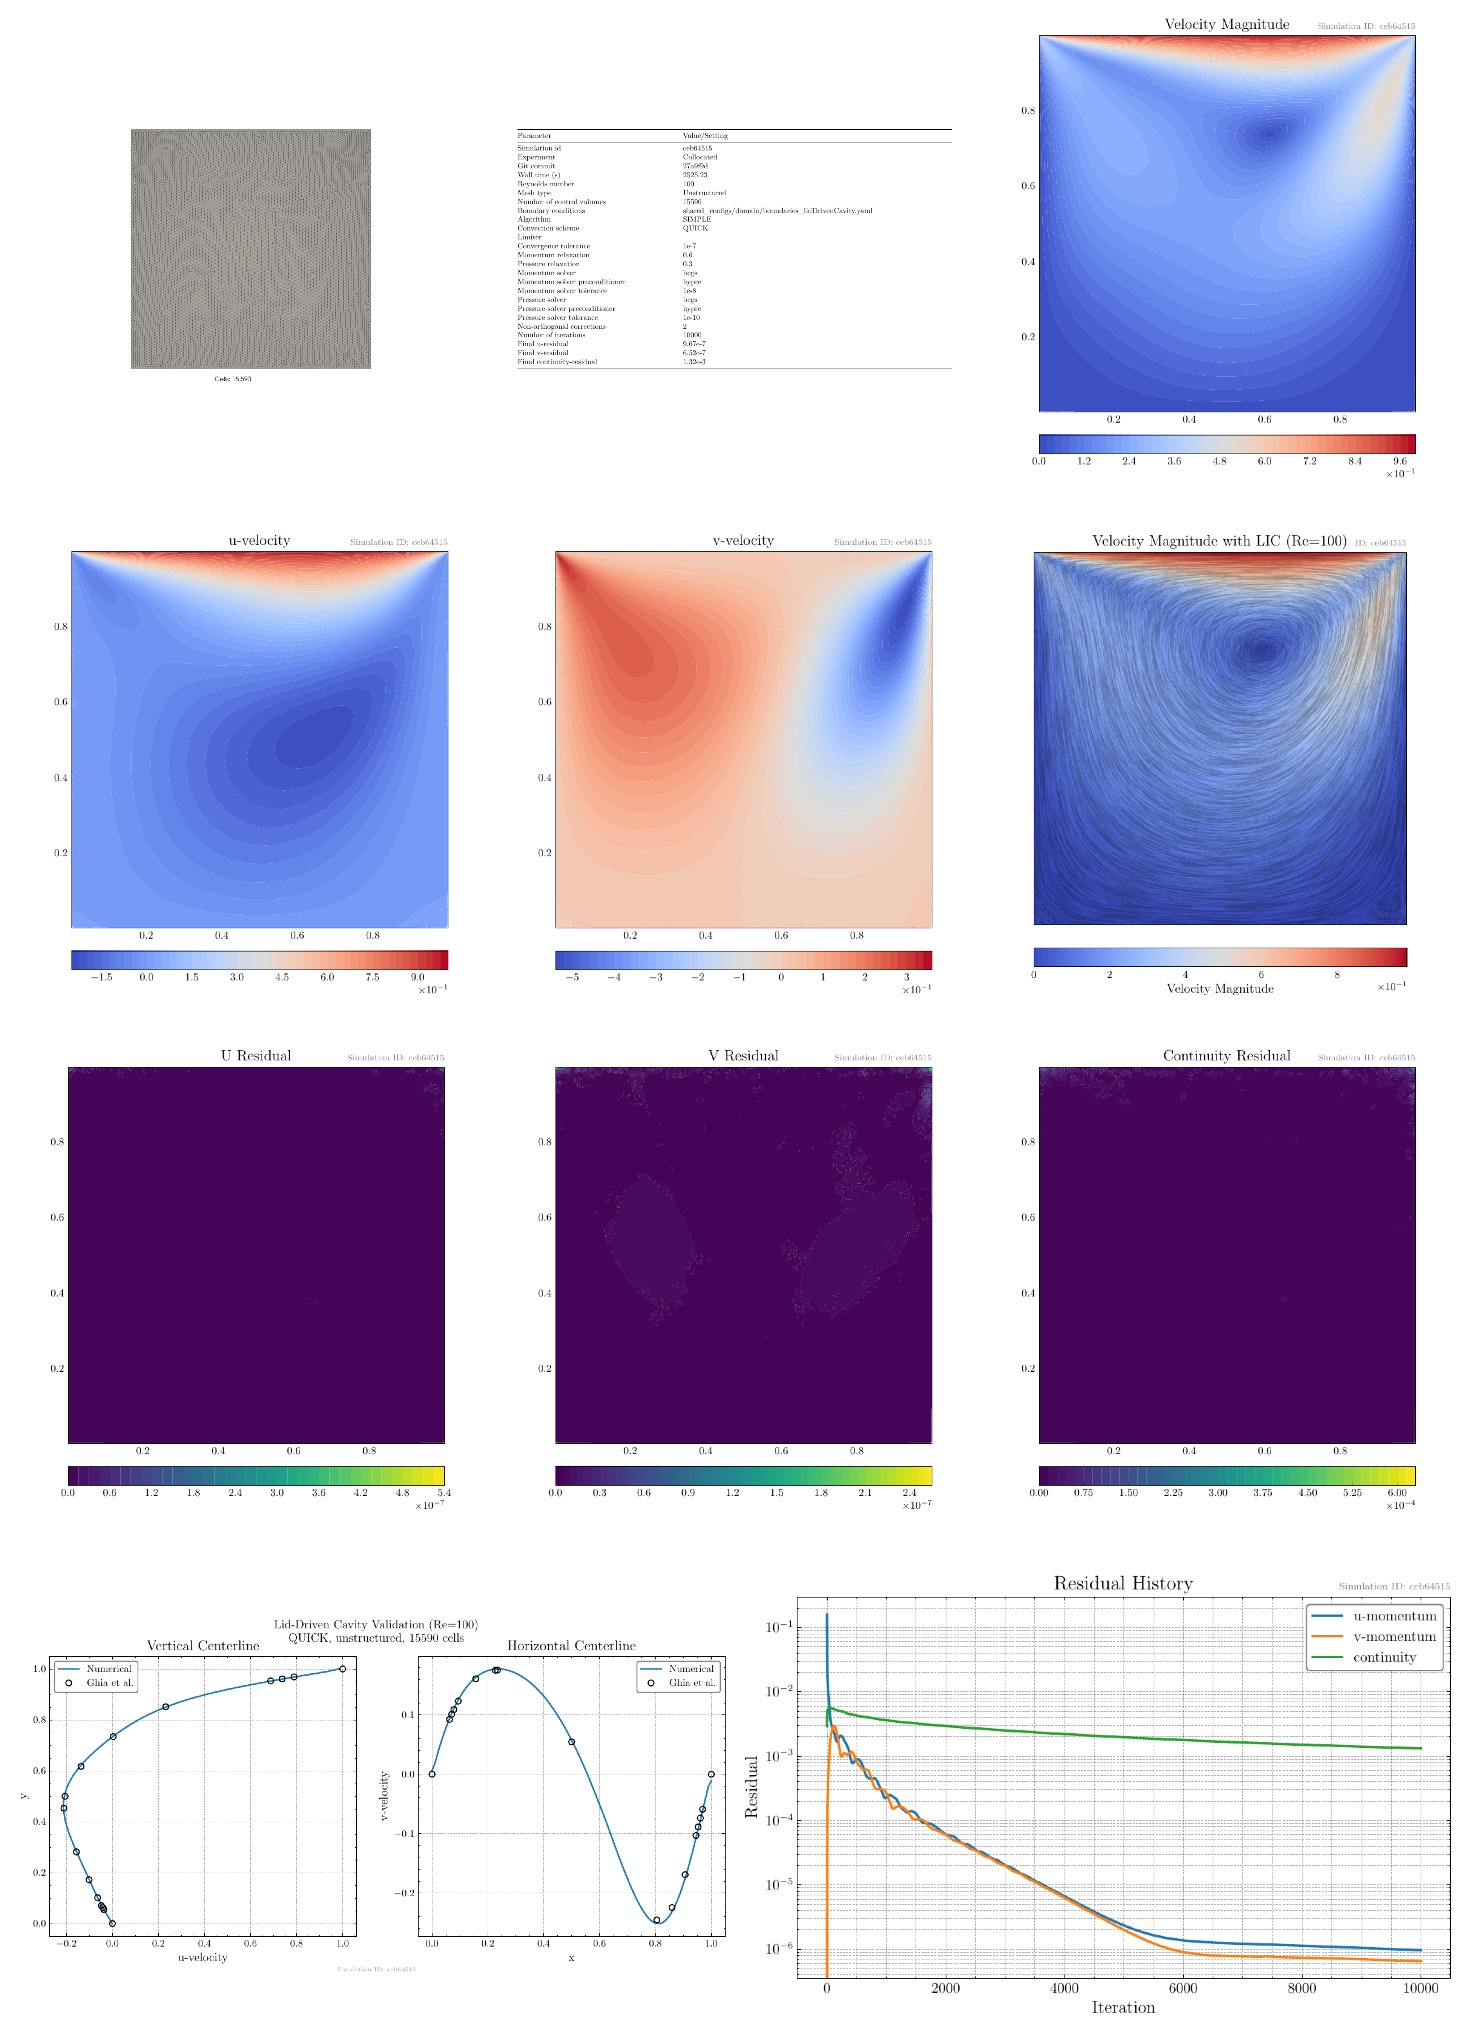
\includegraphics[width=0.85\linewidth]{AppendixPlots/lidDrivenCavity/Re_100/medium/lidDrivenCavity_Re100_unstructured_medium_QUICK_ceb64515.pdf}
    \caption{Liddrivencavity simulation at Re=100 using unstructured medium mesh with QUICK discretization scheme (Simulation ID: ceb64515)}
    \label{sim.ldc.re100.unstruct.med.quick}
\end{figure}

\paragraph*{Unstructured Mesh with TVD Scheme}
\addcontentsline{toc}{paragraph}{Unstructured Mesh with TVD Scheme}
\label{para:liddrivencavity_re100_medium_unstructured_TVD}

\begin{figure}[H]
    \centering
    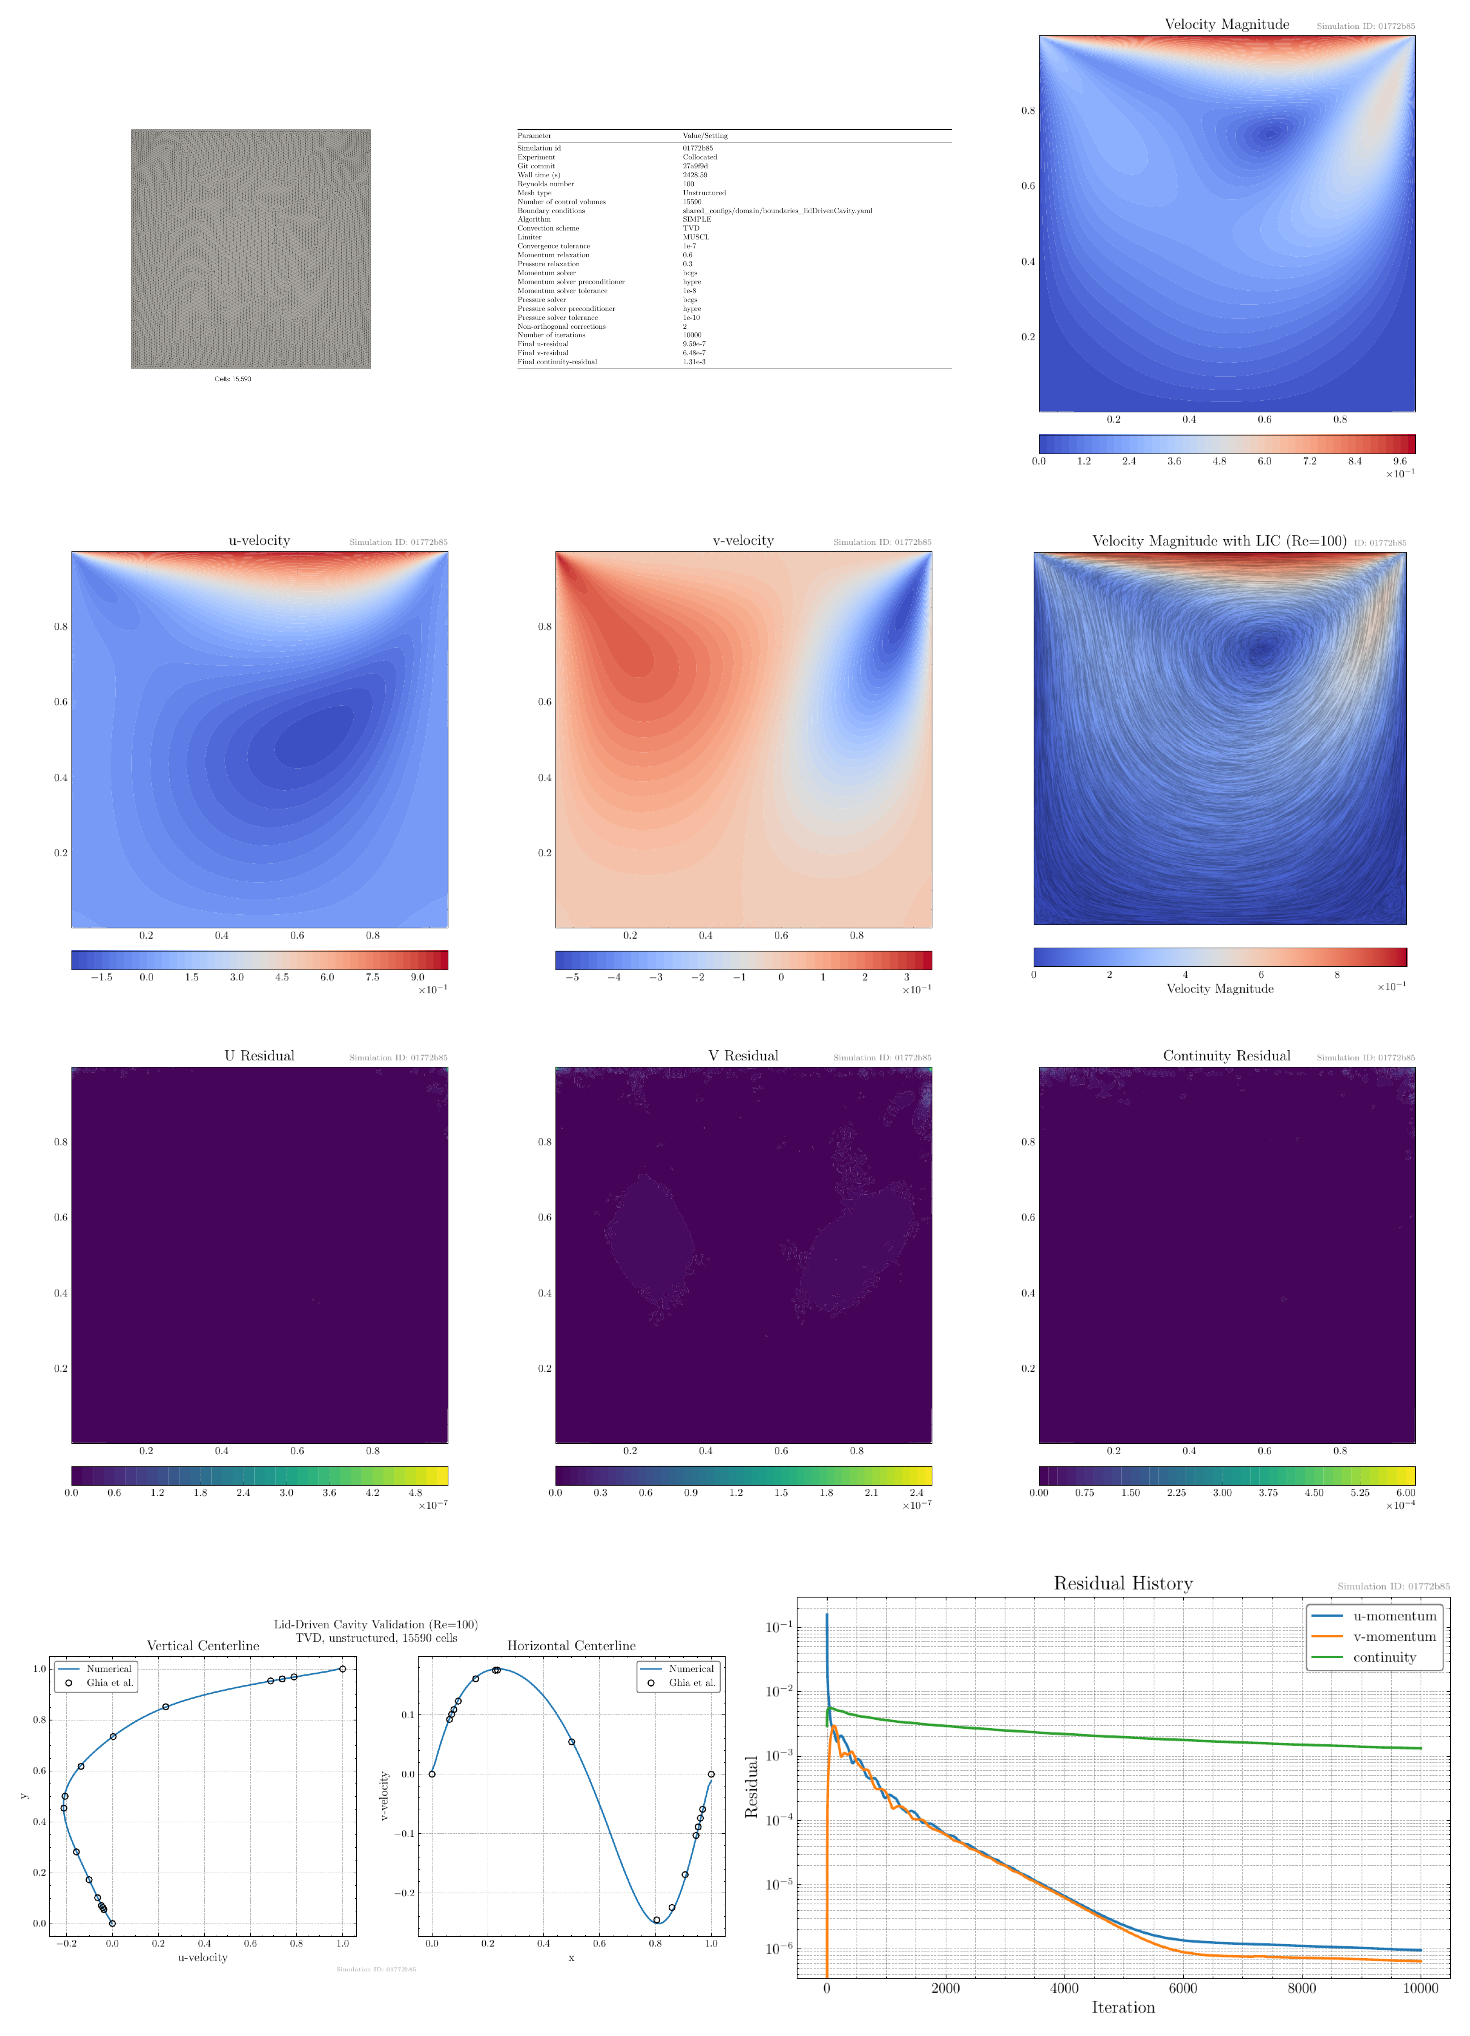
\includegraphics[width=0.85\linewidth]{AppendixPlots/lidDrivenCavity/Re_100/medium/lidDrivenCavity_Re100_unstructured_medium_TVD_01772b85.pdf}
    \caption{Liddrivencavity simulation at Re=100 using unstructured medium mesh with TVD discretization scheme (Simulation ID: 01772b85)}
    \label{sim.ldc.re100.unstruct.med.tvd}
\end{figure}

\paragraph*{Unstructured Mesh with Upwind Scheme}
\addcontentsline{toc}{paragraph}{Unstructured Mesh with Upwind Scheme}
\label{para:liddrivencavity_re100_medium_unstructured_Upwind}

\begin{figure}[H]
    \centering
    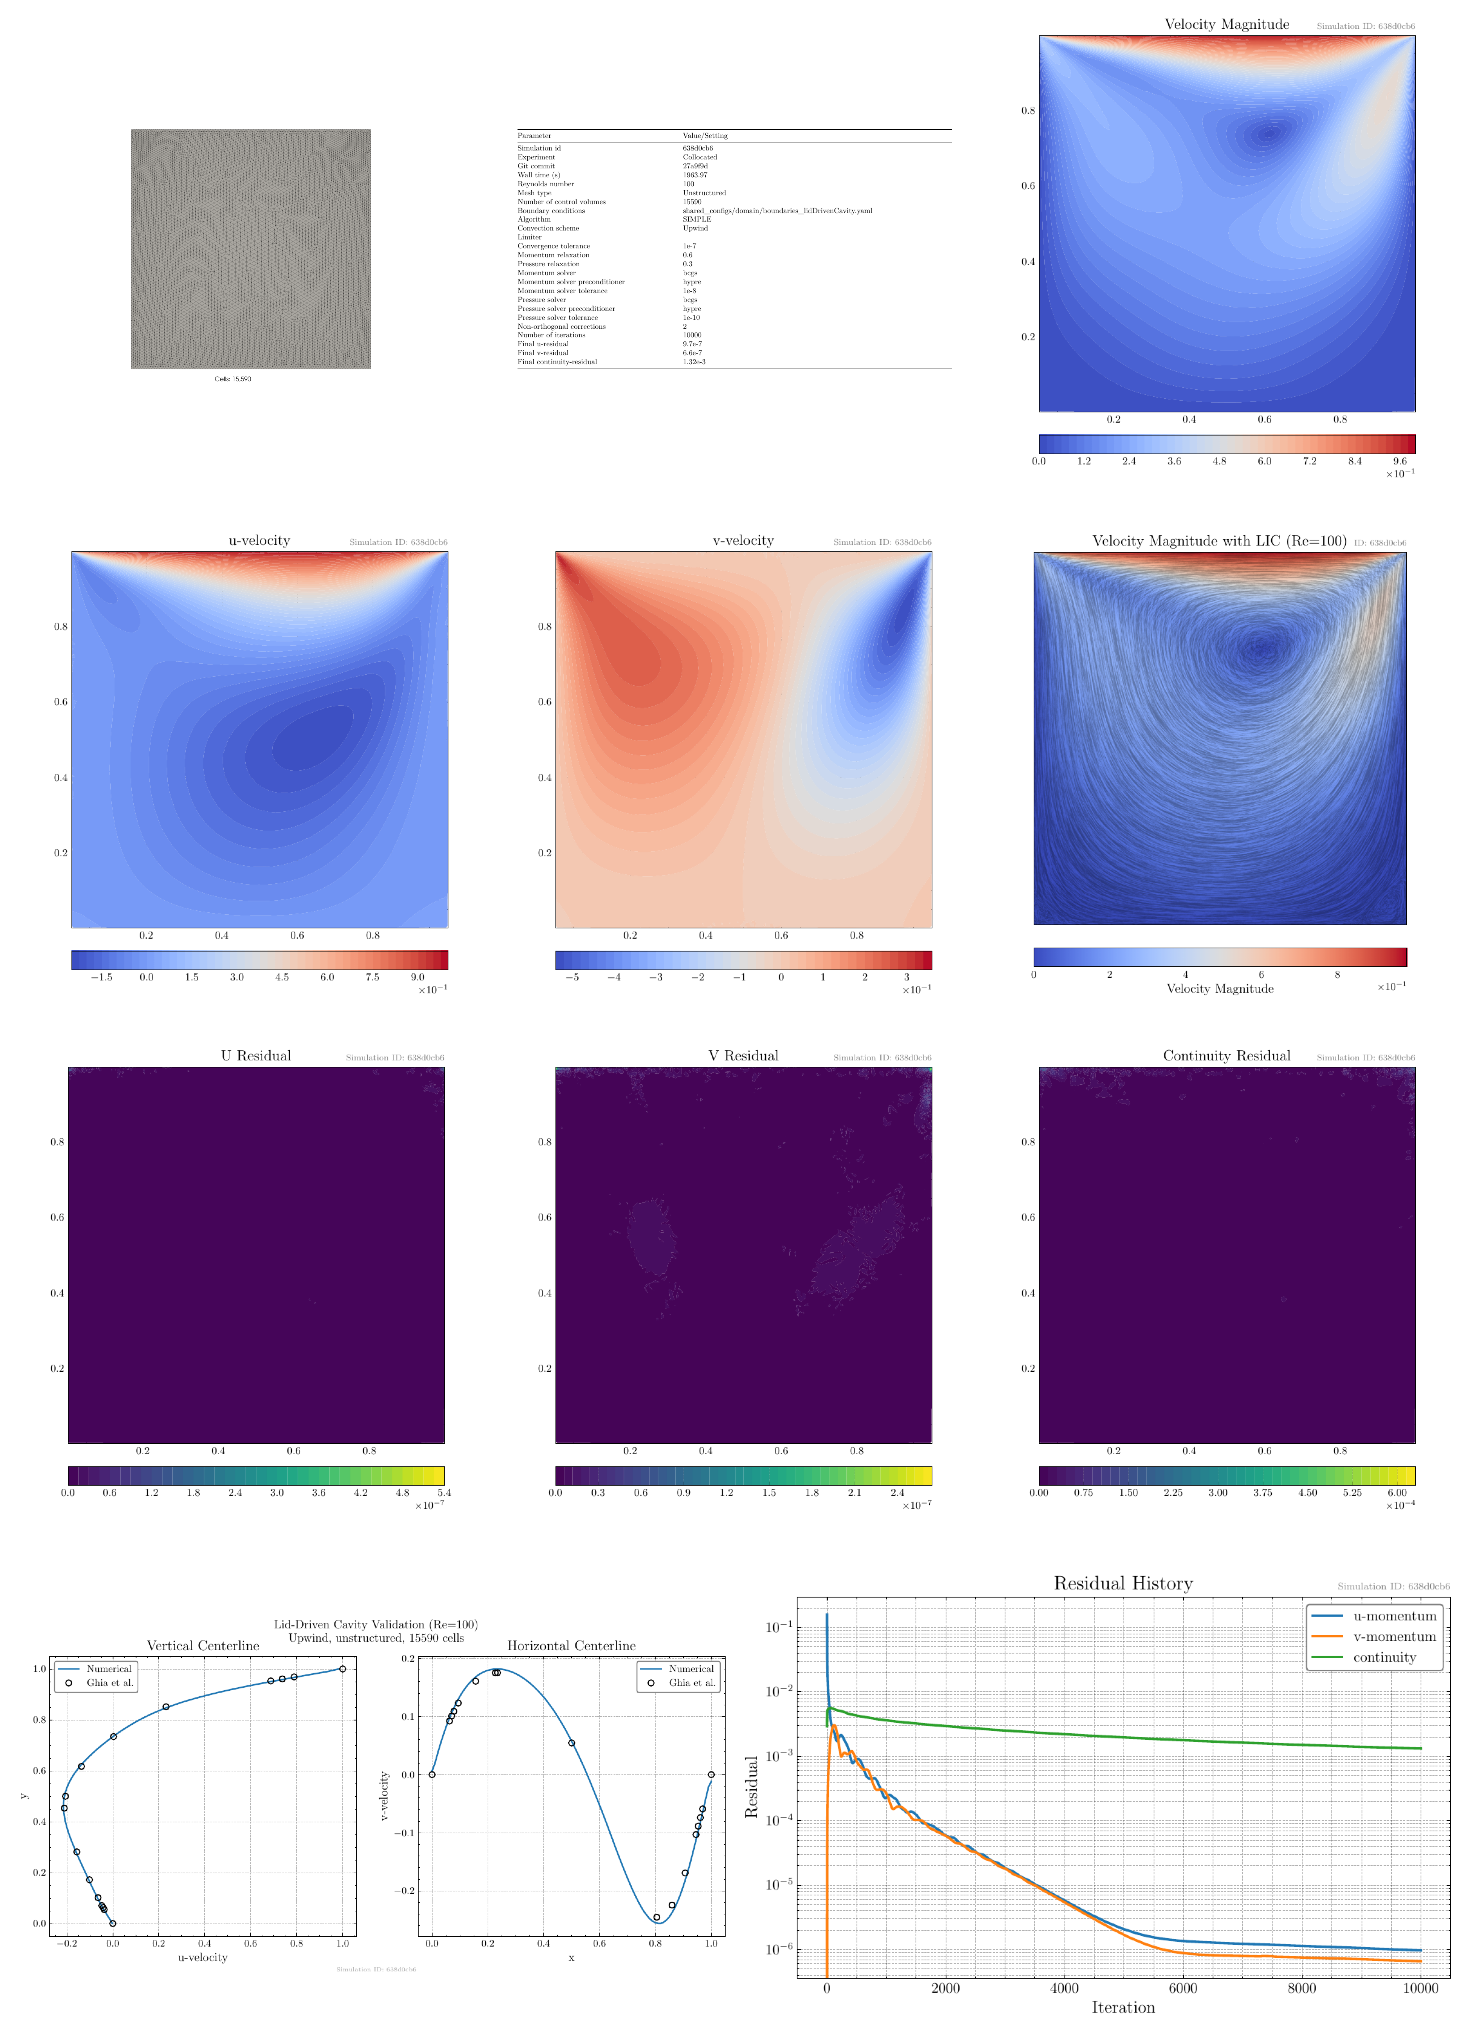
\includegraphics[width=0.85\linewidth]{AppendixPlots/lidDrivenCavity/Re_100/medium/lidDrivenCavity_Re100_unstructured_medium_Upwind_638d0cb6.pdf}
    \caption{Liddrivencavity simulation at Re=100 using unstructured medium mesh with Upwind discretization scheme (Simulation ID: 638d0cb6)}
    \label{sim.ldc.re100.unstruct.med.upwind}
\end{figure}

\clearpage

\subsubsection*{Fine Mesh}
\addcontentsline{toc}{subsubsection}{Fine Mesh}
\label{subsubsec:liddrivencavity_re100_fine}

\paragraph*{Uniform Mesh with QUICK Scheme}
\addcontentsline{toc}{paragraph}{Uniform Mesh with QUICK Scheme}
\label{para:liddrivencavity_re100_fine_uniform_QUICK}

\begin{figure}[H]
    \centering
    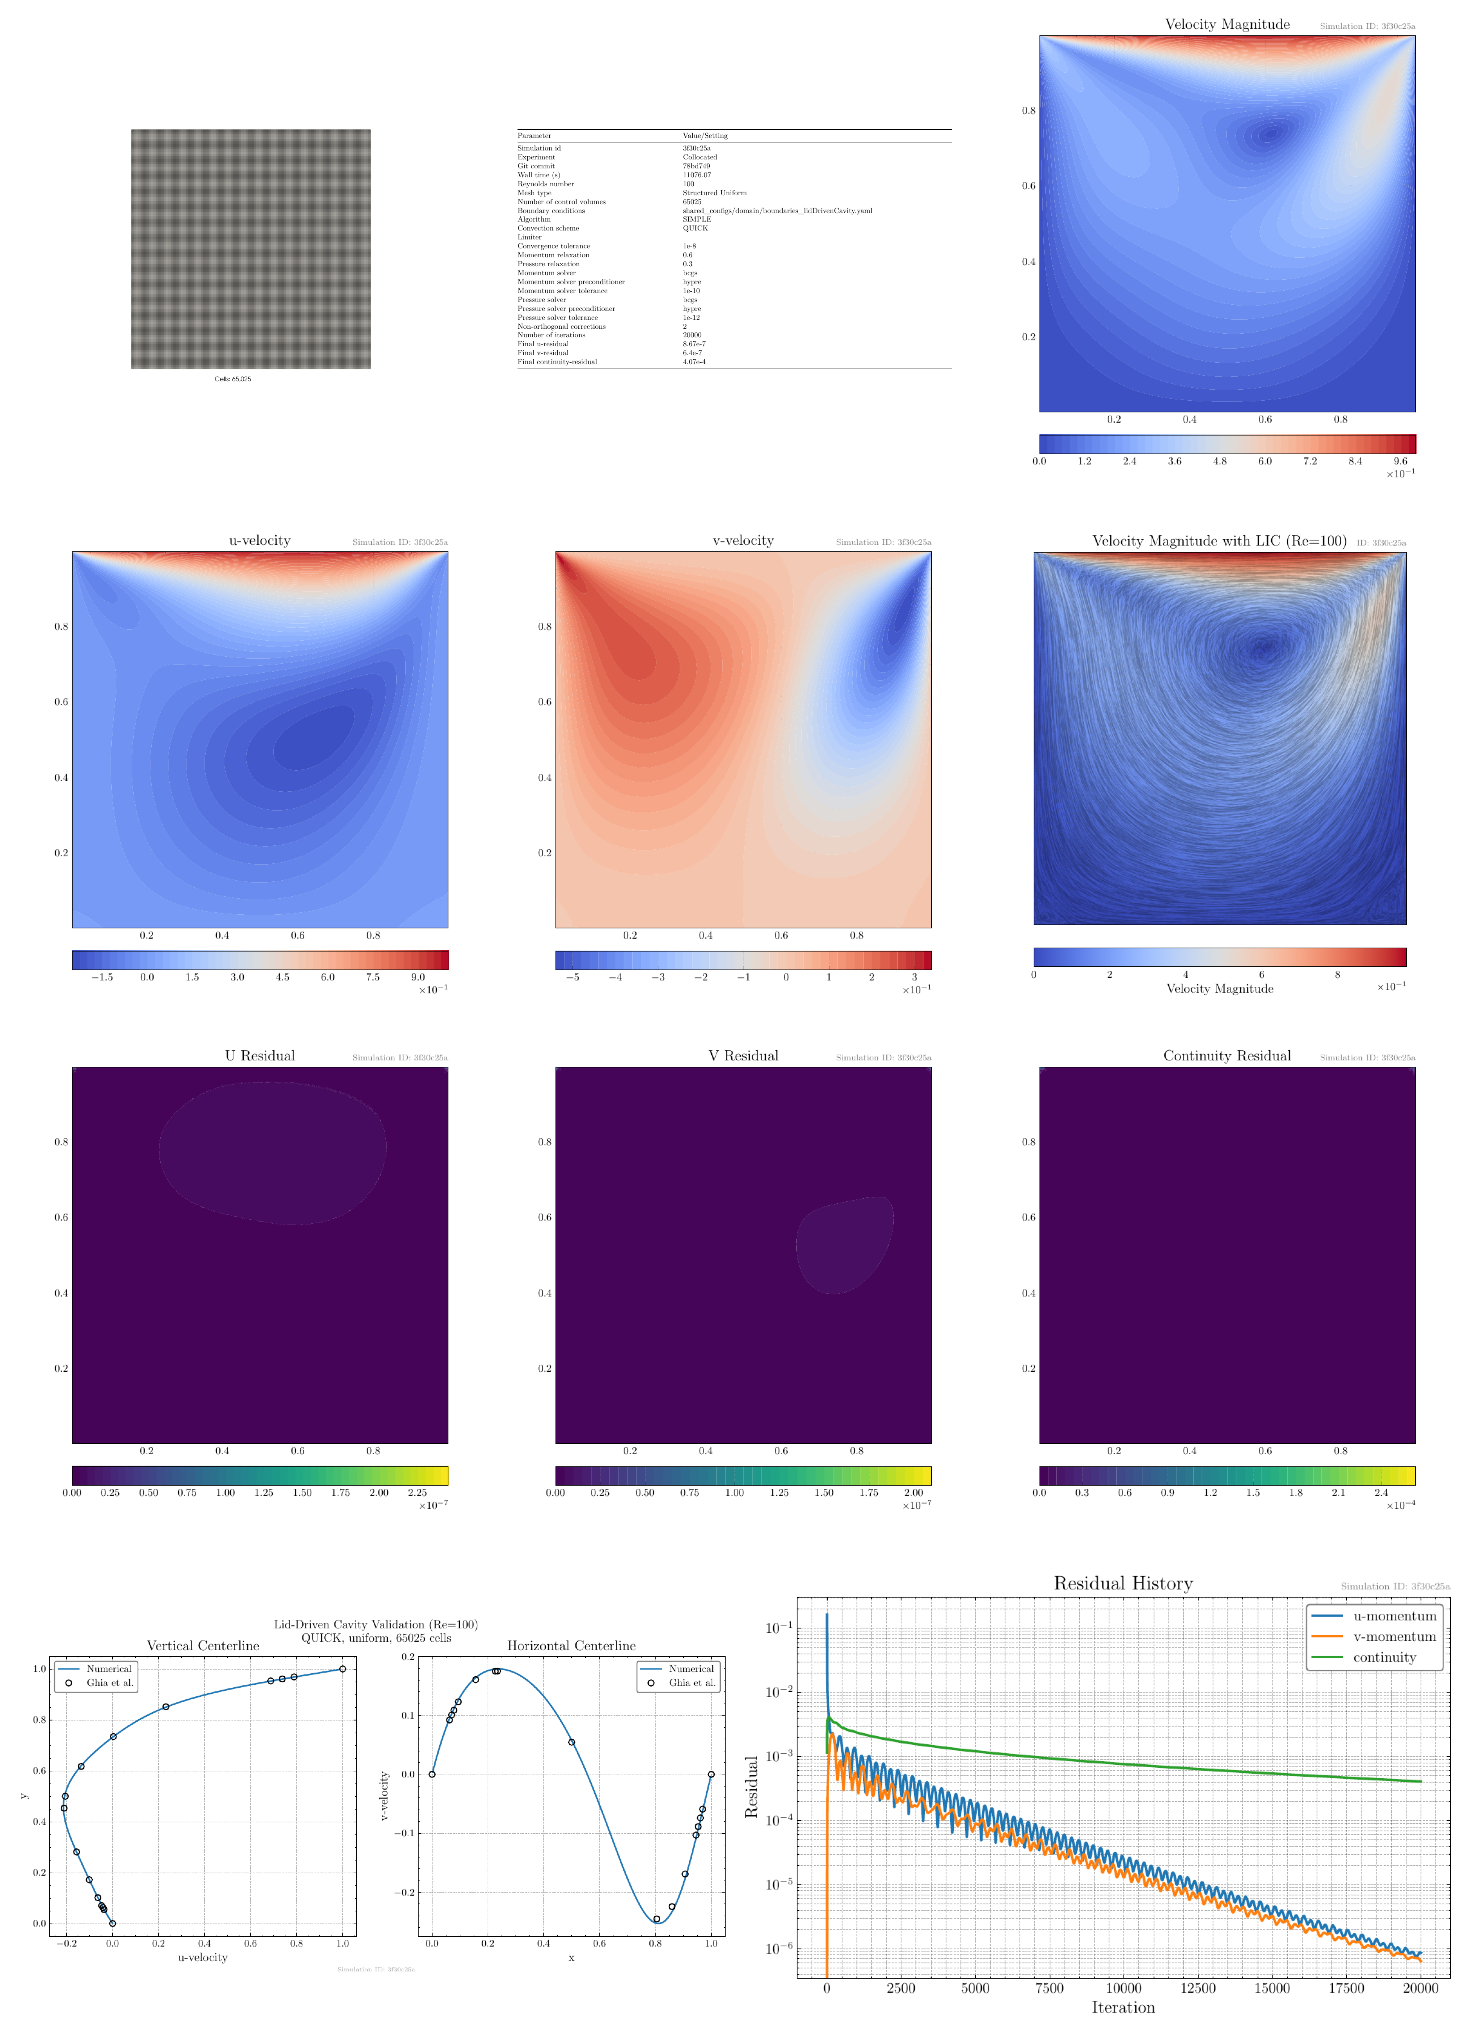
\includegraphics[width=0.85\linewidth]{AppendixPlots/lidDrivenCavity/Re_100/fine/lidDrivenCavity_Re100_uniform_fine_QUICK_3f30c25a.pdf}
    \caption{Liddrivencavity simulation at Re=100 using uniform fine mesh with QUICK discretization scheme (Simulation ID: 3f30c25a)}
    \label{sim.ldc.re100.unif.fine.quick}
\end{figure}

\paragraph*{Uniform Mesh with TVD Scheme}
\addcontentsline{toc}{paragraph}{Uniform Mesh with TVD Scheme}
\label{para:liddrivencavity_re100_fine_uniform_TVD}

\begin{figure}[H]
    \centering
    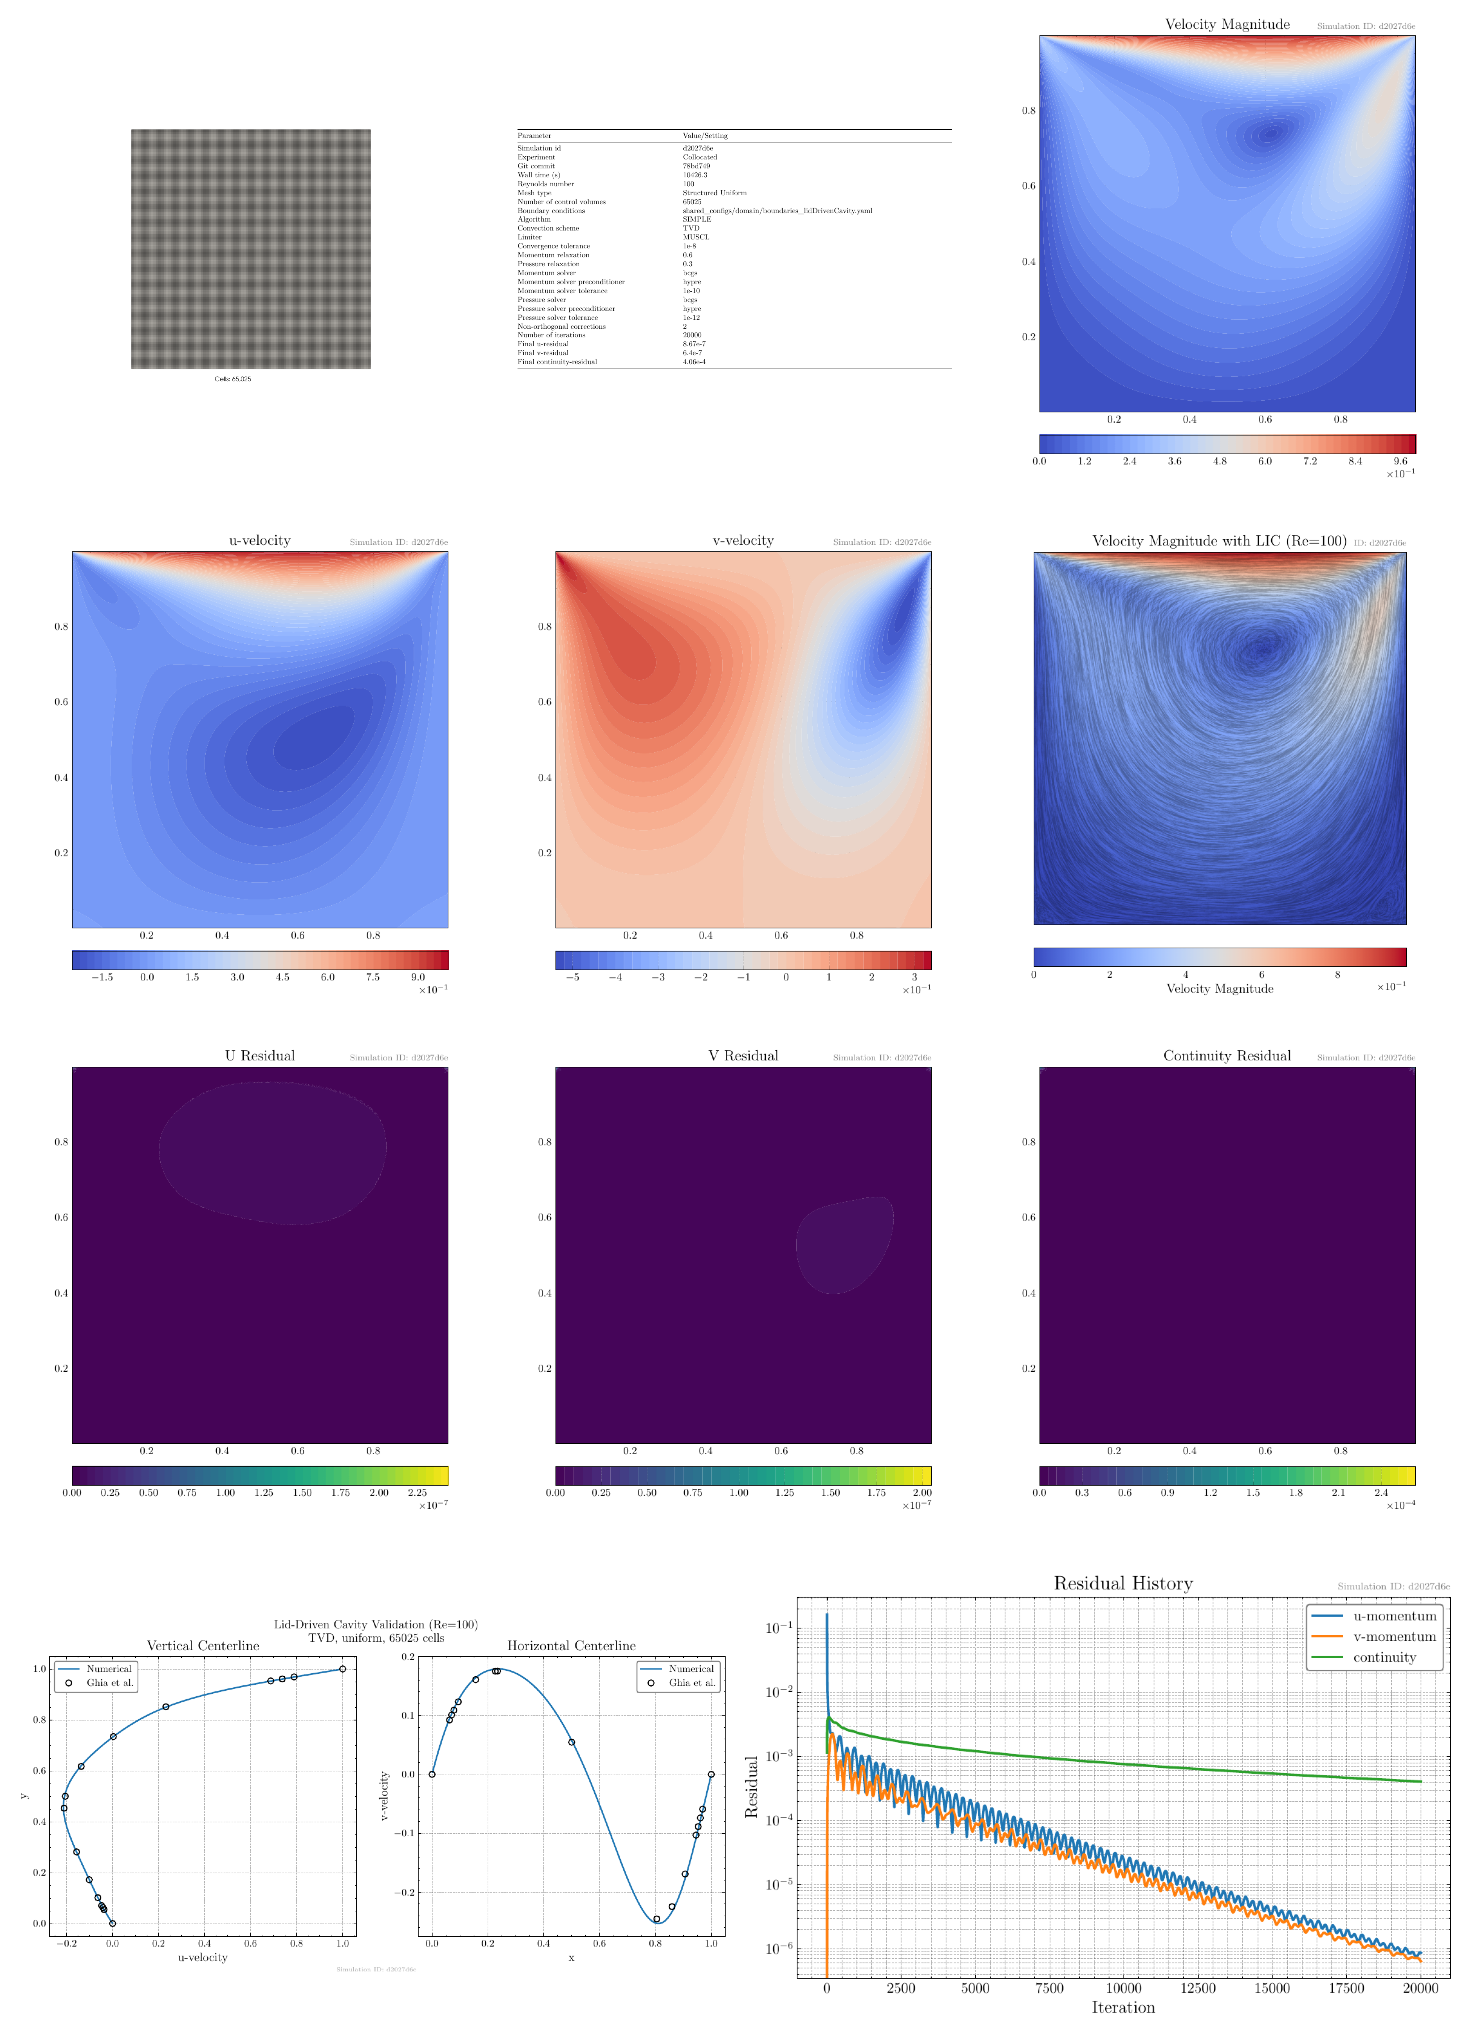
\includegraphics[width=0.85\linewidth]{AppendixPlots/lidDrivenCavity/Re_100/fine/lidDrivenCavity_Re100_uniform_fine_TVD_d2027d6e.pdf}
    \caption{Liddrivencavity simulation at Re=100 using uniform fine mesh with TVD discretization scheme (Simulation ID: d2027d6e)}
    \label{sim.ldc.re100.unif.fine.tvd}
\end{figure}

\paragraph*{Unstructured Mesh with QUICK Scheme}
\addcontentsline{toc}{paragraph}{Unstructured Mesh with QUICK Scheme}
\label{para:liddrivencavity_re100_fine_unstructured_QUICK}

\begin{figure}[H]
    \centering
    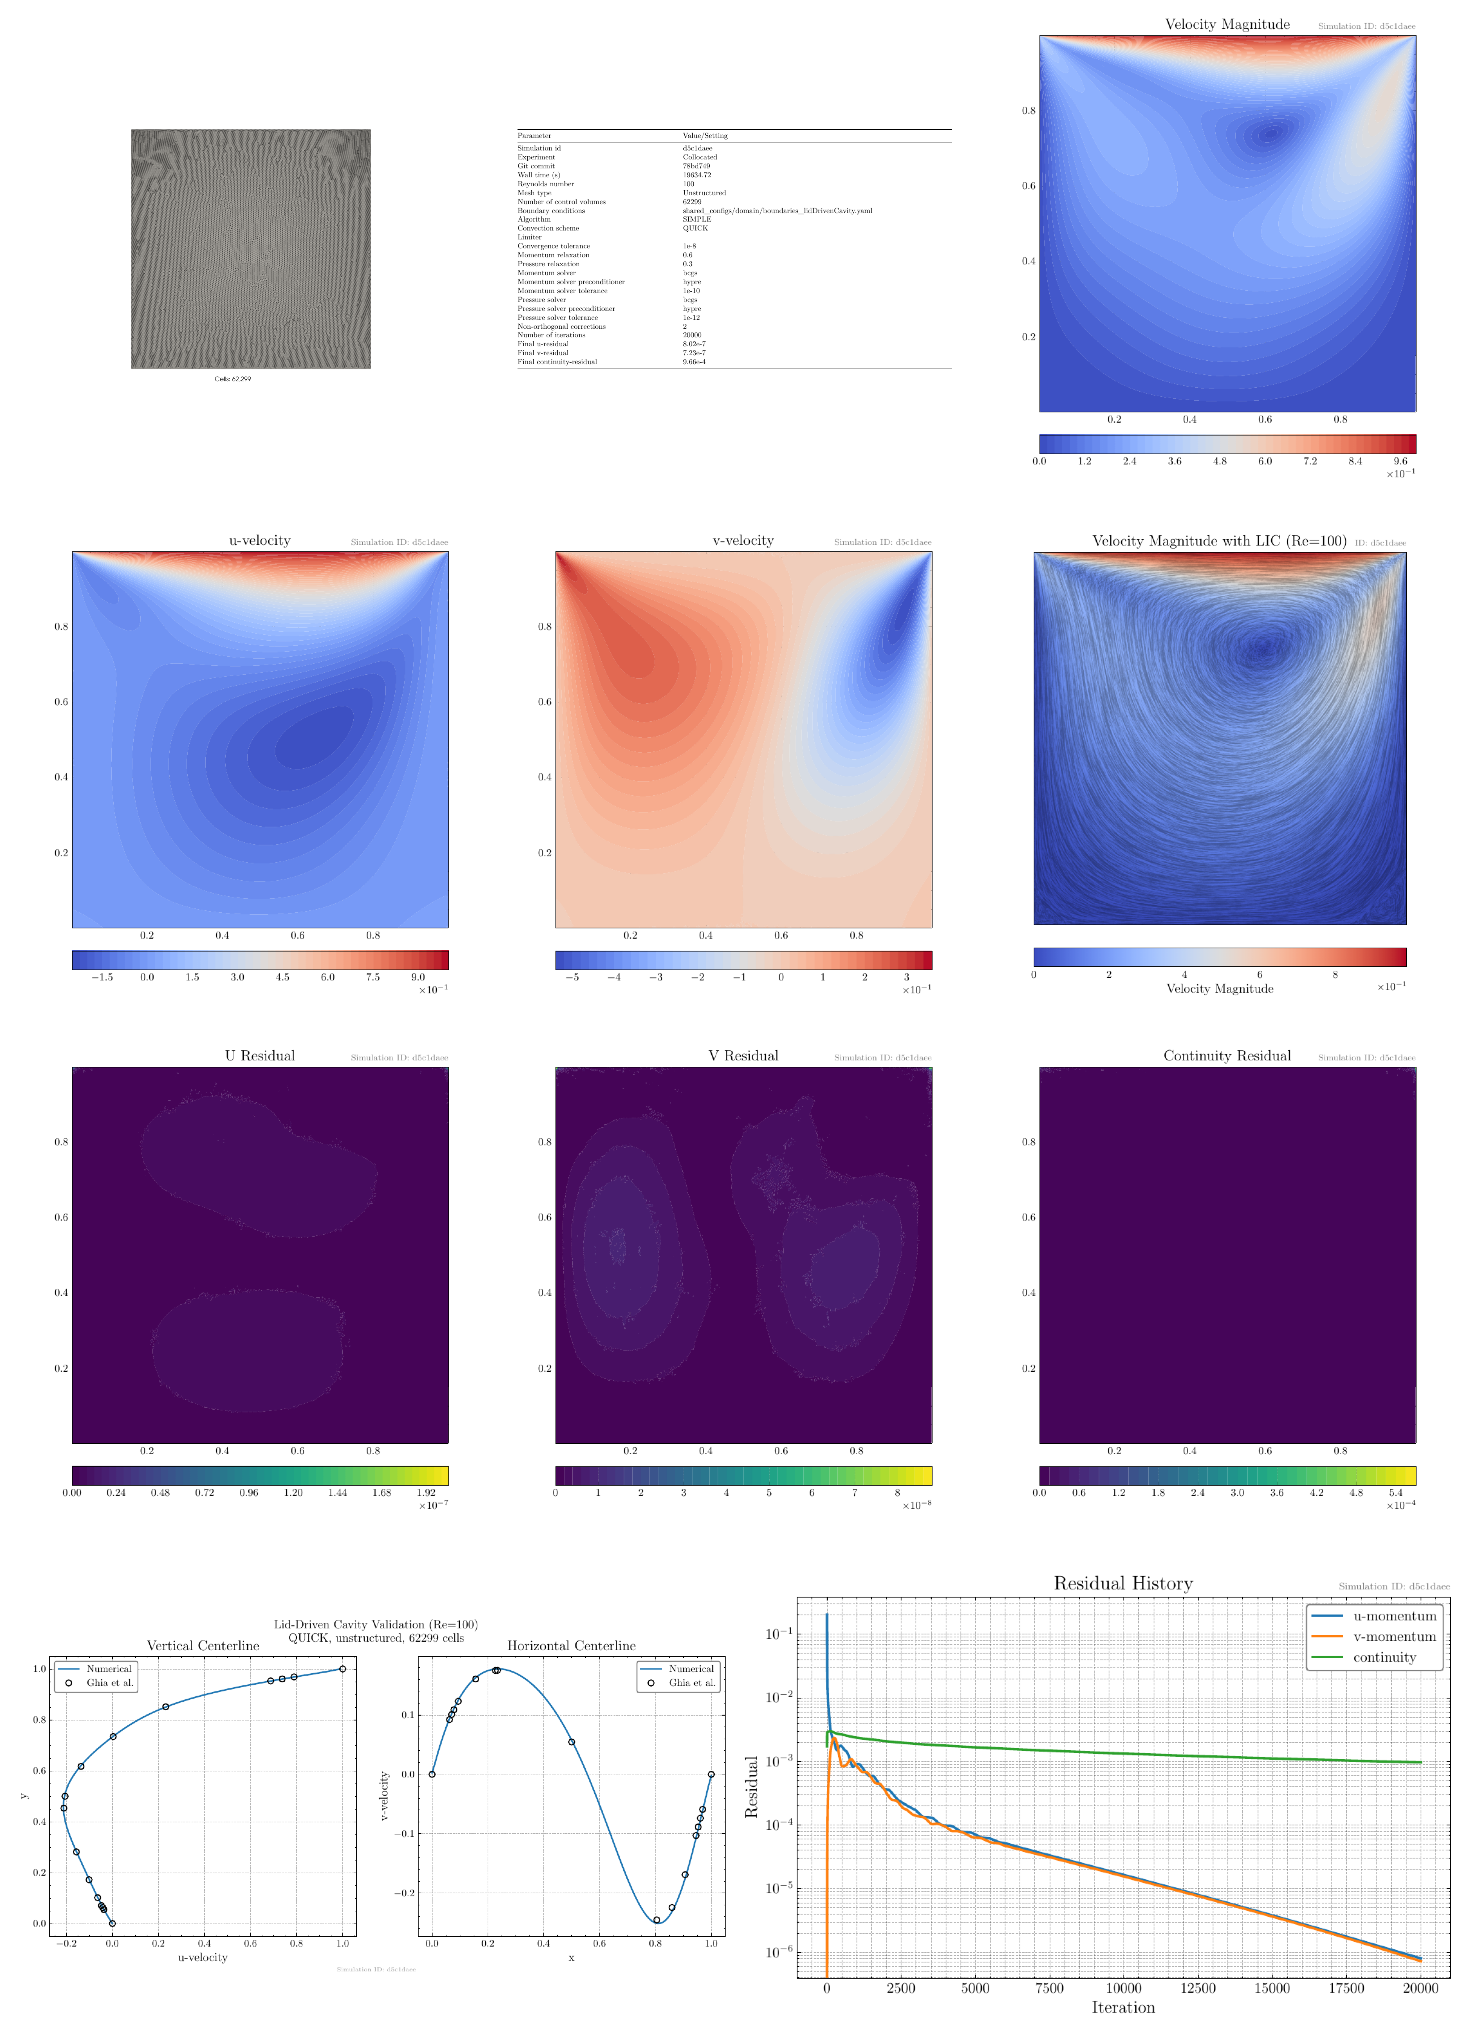
\includegraphics[width=0.85\linewidth]{AppendixPlots/lidDrivenCavity/Re_100/fine/lidDrivenCavity_Re100_unstructured_fine_QUICK_d5c1daee.pdf}
    \caption{Liddrivencavity simulation at Re=100 using unstructured fine mesh with QUICK discretization scheme (Simulation ID: d5c1daee)}
    \label{sim.ldc.re100.unstruct.fine.quick}
\end{figure}

\paragraph*{Unstructured Mesh with TVD Scheme}
\addcontentsline{toc}{paragraph}{Unstructured Mesh with TVD Scheme}
\label{para:liddrivencavity_re100_fine_unstructured_TVD}

\begin{figure}[H]
    \centering
    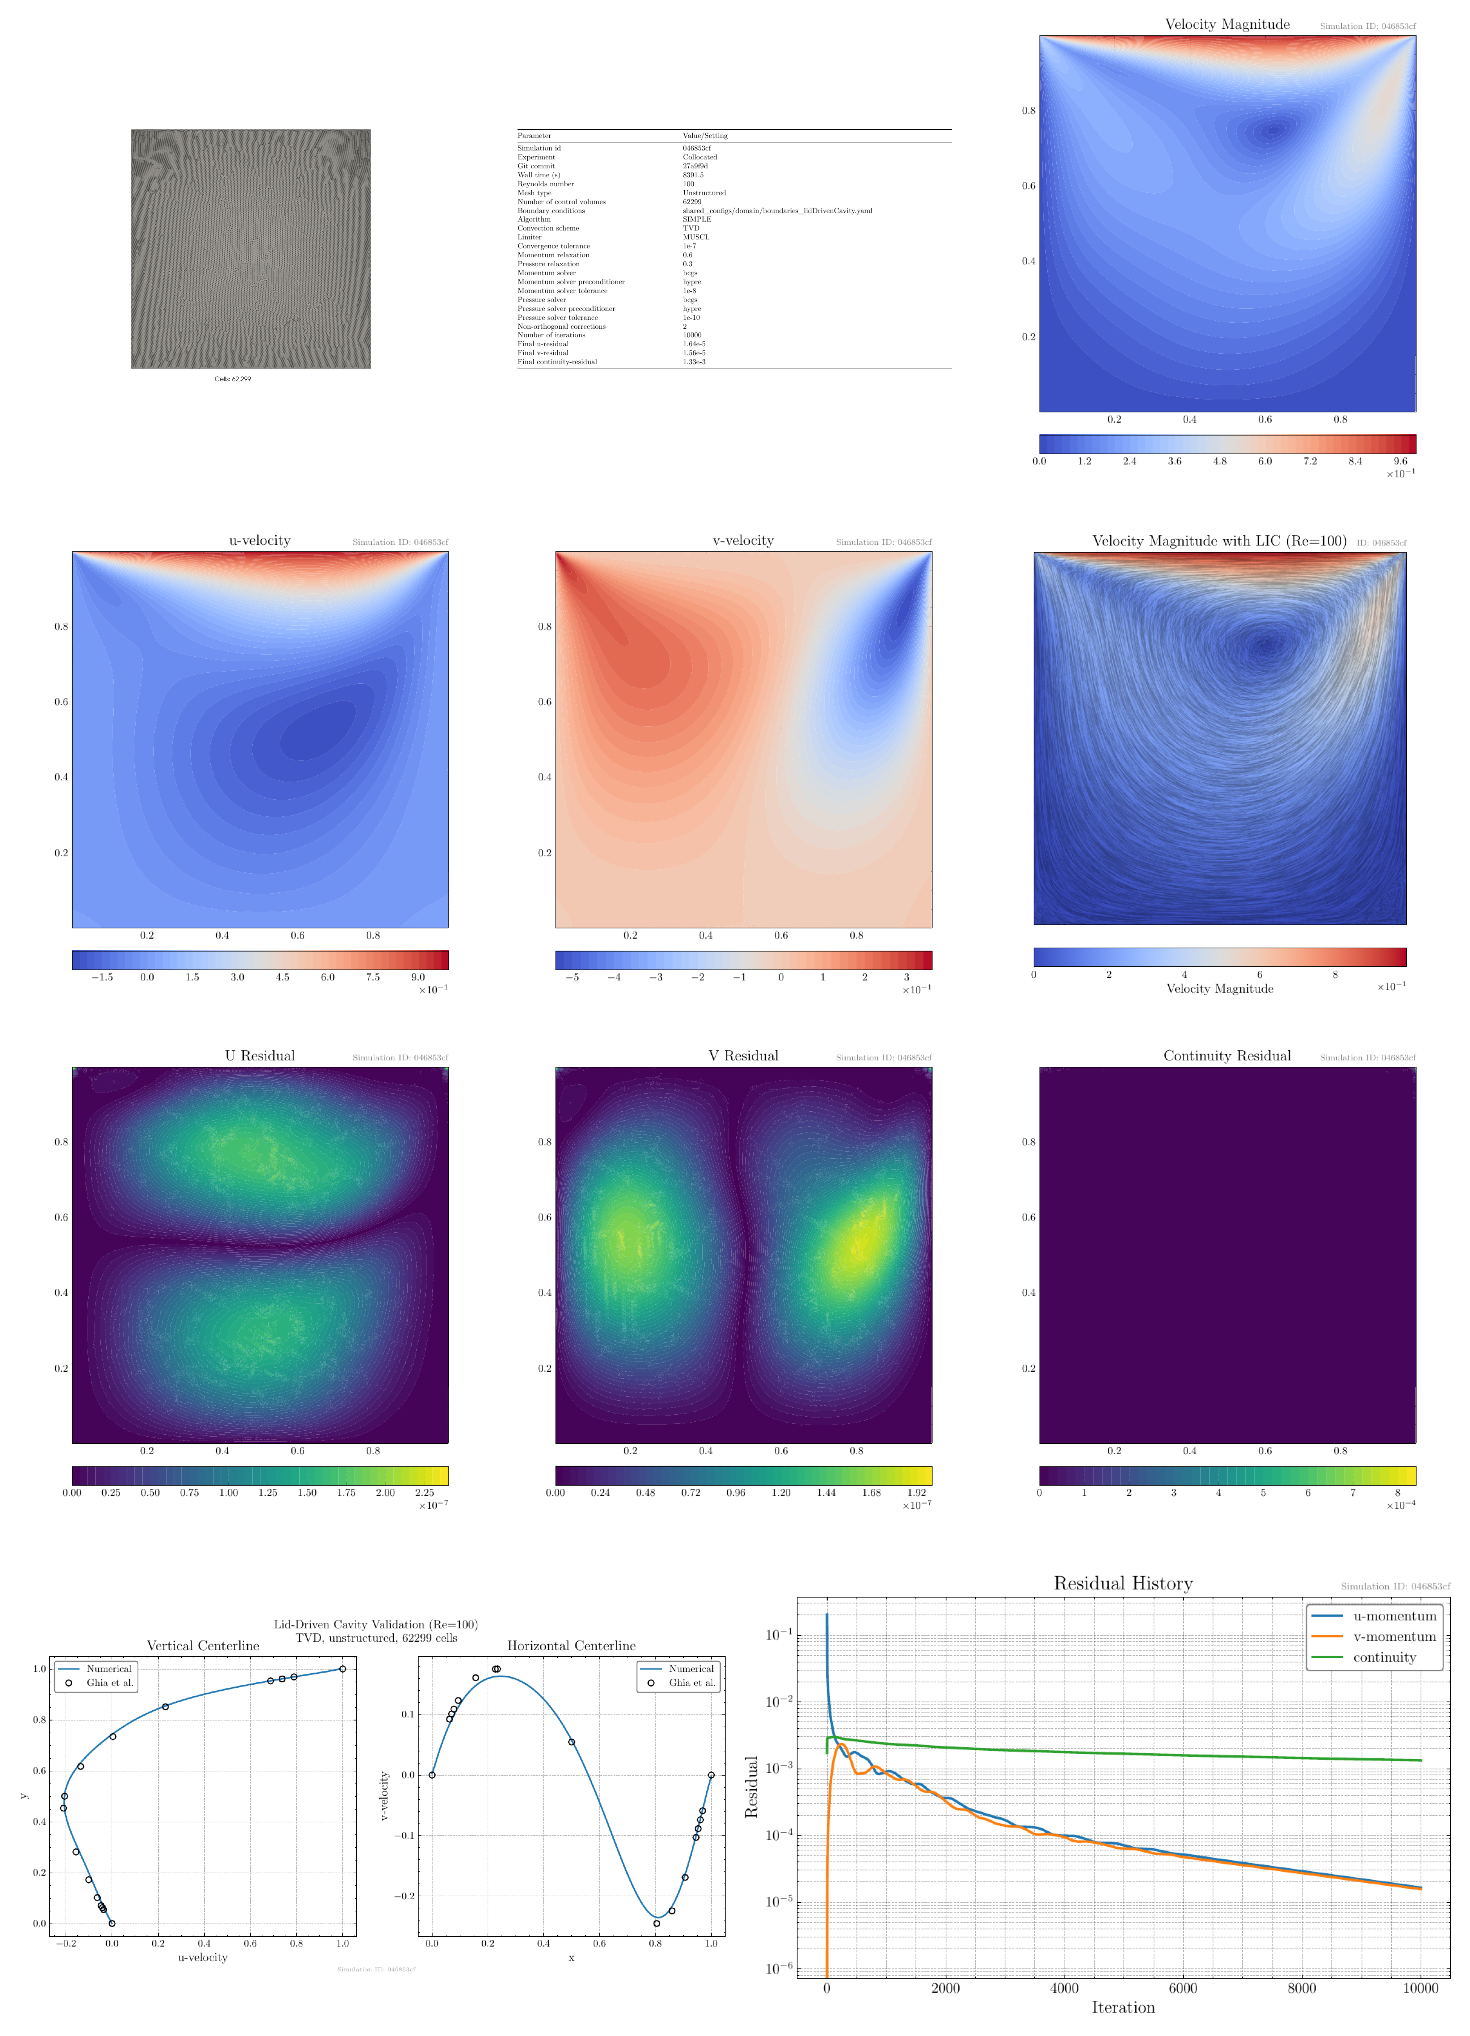
\includegraphics[width=0.85\linewidth]{AppendixPlots/lidDrivenCavity/Re_100/fine/lidDrivenCavity_Re100_unstructured_fine_TVD_046853cf.pdf}
    \caption{Liddrivencavity simulation at Re=100 using unstructured fine mesh with TVD discretization scheme (Simulation ID: 046853cf)}
    \label{sim.ldc.re100.unstruct.fine.tvd}
\end{figure}

\paragraph*{Unstructured Mesh with Upwind Scheme}
\addcontentsline{toc}{paragraph}{Unstructured Mesh with Upwind Scheme}
\label{para:liddrivencavity_re100_fine_unstructured_Upwind}

\begin{figure}[H]
    \centering
    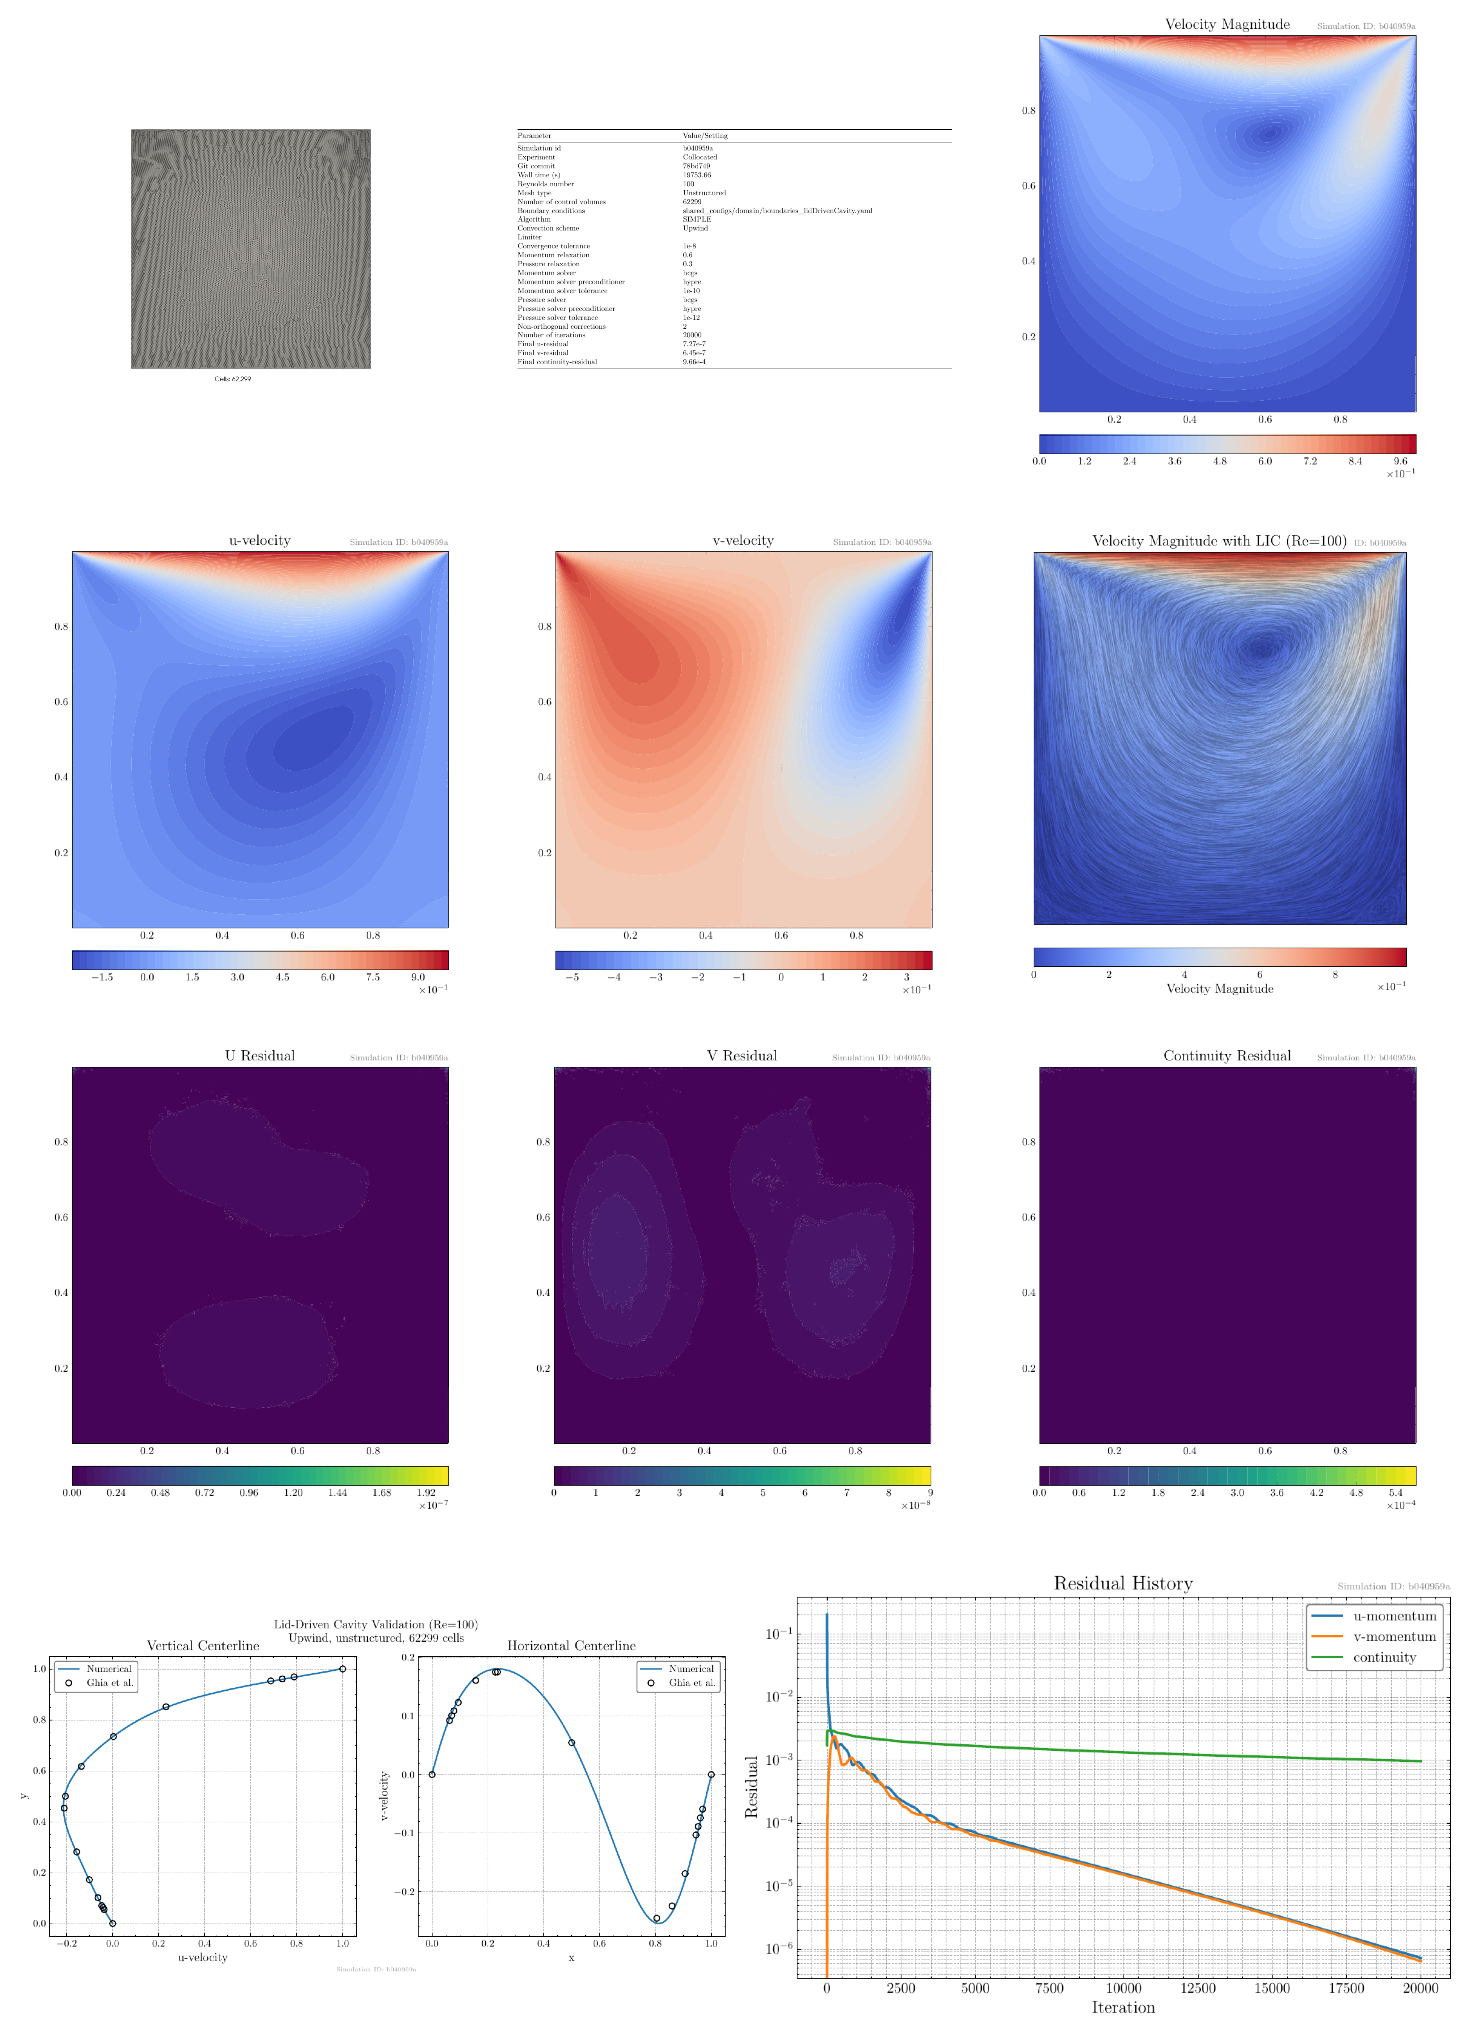
\includegraphics[width=0.85\linewidth]{AppendixPlots/lidDrivenCavity/Re_100/fine/lidDrivenCavity_Re100_unstructured_fine_Upwind_b040959a.pdf}
    \caption{Liddrivencavity simulation at Re=100 using unstructured fine mesh with Upwind discretization scheme (Simulation ID: b040959a)}
    \label{sim.ldc.re100.unstruct.fine.upwind}
\end{figure}

\clearpage

\subsubsection*{127X127 Mesh}
\addcontentsline{toc}{subsubsection}{127X127 Mesh}
\label{subsubsec:liddrivencavity_re100_127x127}

\paragraph*{Structured Mesh with Power Law Scheme}
\addcontentsline{toc}{paragraph}{Structured Mesh with Power Law Scheme}
\label{para:liddrivencavity_re100_127x127_structured_Power Law}

\begin{figure}[H]
    \centering
    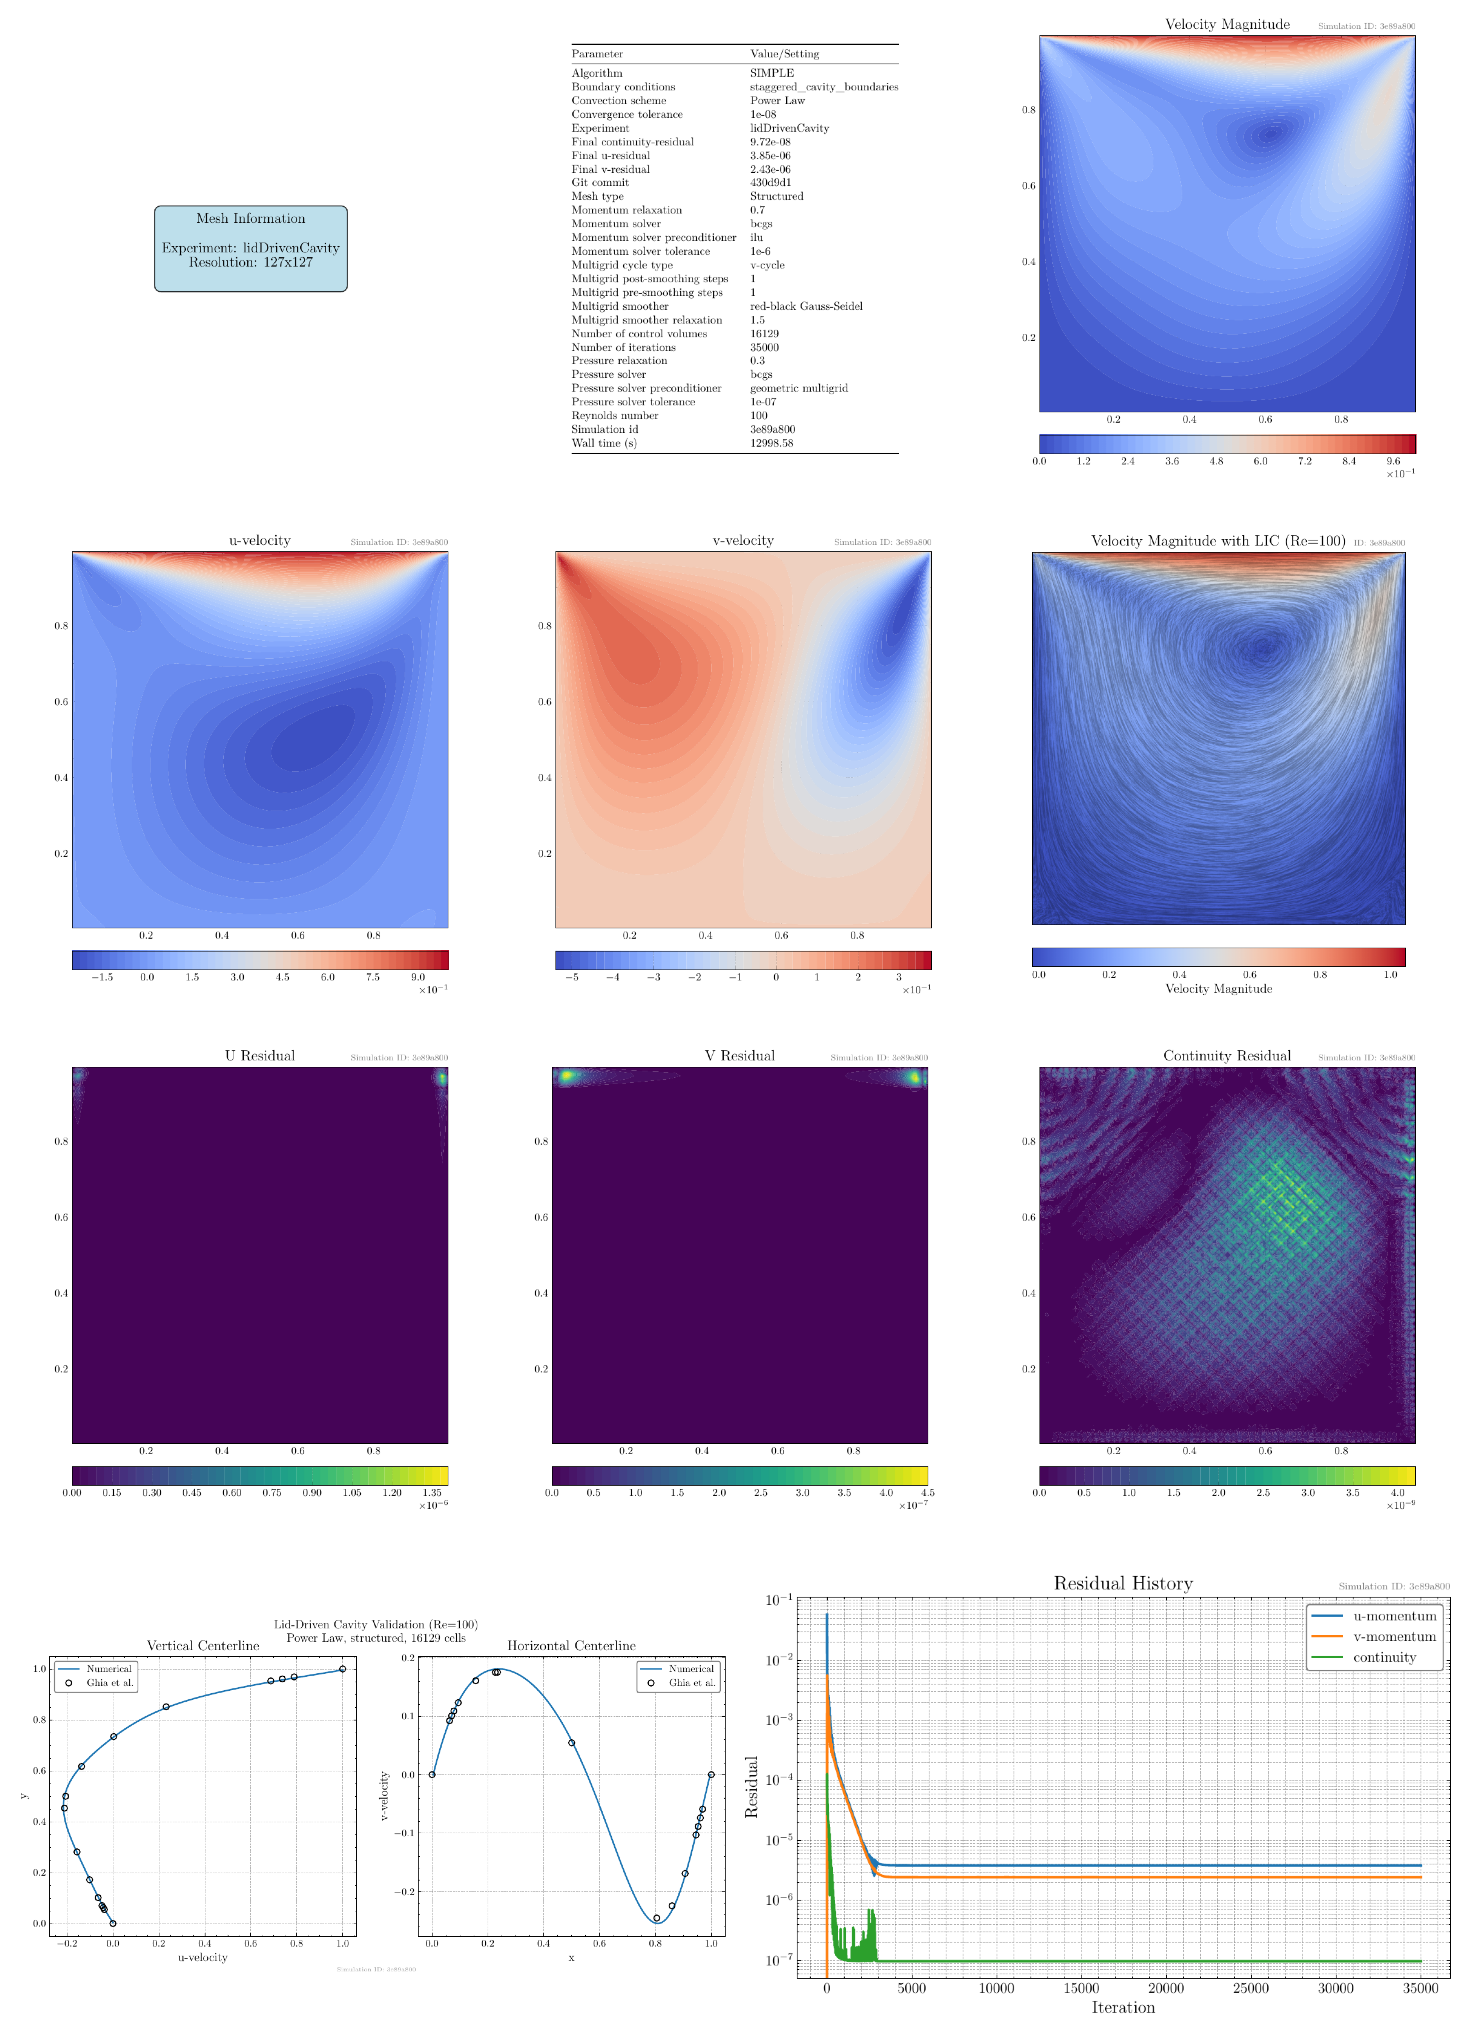
\includegraphics[width=0.85\linewidth]{AppendixPlots/lidDrivenCavity/Re_100/127x127/lidDrivenCavity_Re100_structured_127x127_Power Law_3e89a800.pdf}
    \caption{Liddrivencavity simulation at Re=100 using structured 127x127 (medium) mesh with Power Law discretization scheme (Simulation ID: 3e89a800)}
    \label{sim.ldc.re100.struct.med.powe}
\end{figure}

\subsection*{Reynolds Number 400}
\addcontentsline{toc}{subsection}{Reynolds Number 400}
\label{subsec:liddrivencavity_re400}

\subsubsection*{Coarse Mesh}
\addcontentsline{toc}{subsubsection}{Coarse Mesh}
\label{subsubsec:liddrivencavity_re400_coarse}

\paragraph*{Uniform Mesh with Upwind Scheme}
\addcontentsline{toc}{paragraph}{Uniform Mesh with Upwind Scheme}
\label{para:liddrivencavity_re400_coarse_uniform_Upwind}

\begin{figure}[H]
    \centering
    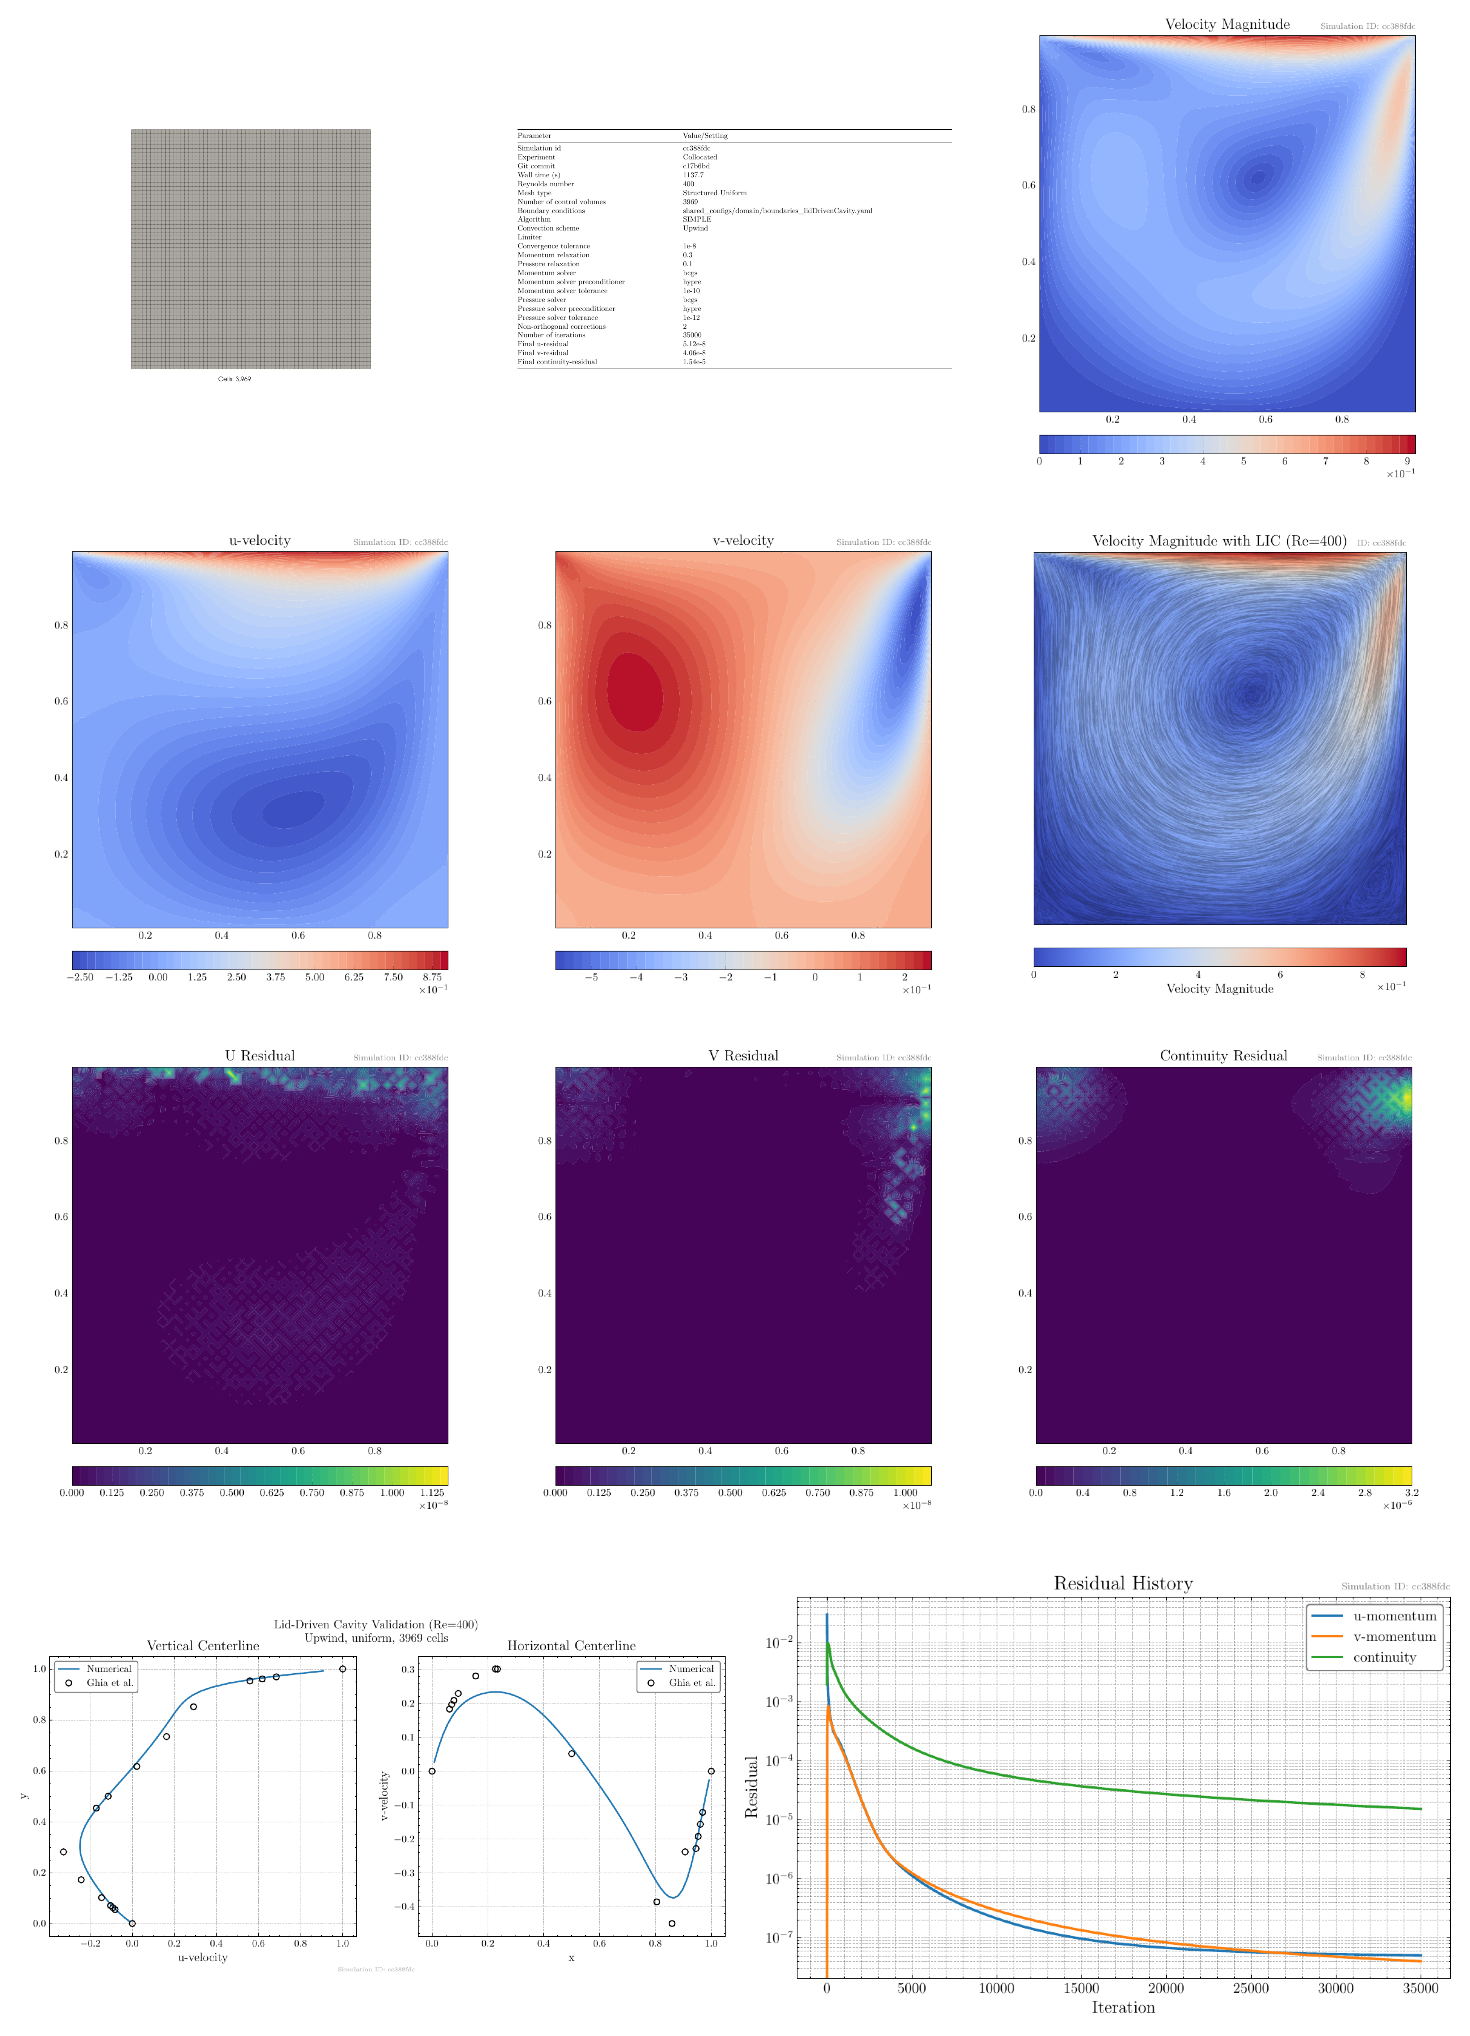
\includegraphics[width=0.85\linewidth]{AppendixPlots/lidDrivenCavity/Re_400/coarse/lidDrivenCavity_Re400_uniform_coarse_Upwind_cc388fdc.pdf}
    \caption{Liddrivencavity simulation at Re=400 using uniform coarse mesh with Upwind discretization scheme (Simulation ID: cc388fdc)}
    \label{sim.ldc.re400.unif.coarse.upwind}
\end{figure}

\clearpage

\subsubsection*{Medium Mesh}
\addcontentsline{toc}{subsubsection}{Medium Mesh}
\label{subsubsec:liddrivencavity_re400_medium}

\paragraph*{Uniform Mesh with QUICK Scheme}
\addcontentsline{toc}{paragraph}{Uniform Mesh with QUICK Scheme}
\label{para:liddrivencavity_re400_medium_uniform_QUICK}

\begin{figure}[H]
    \centering
    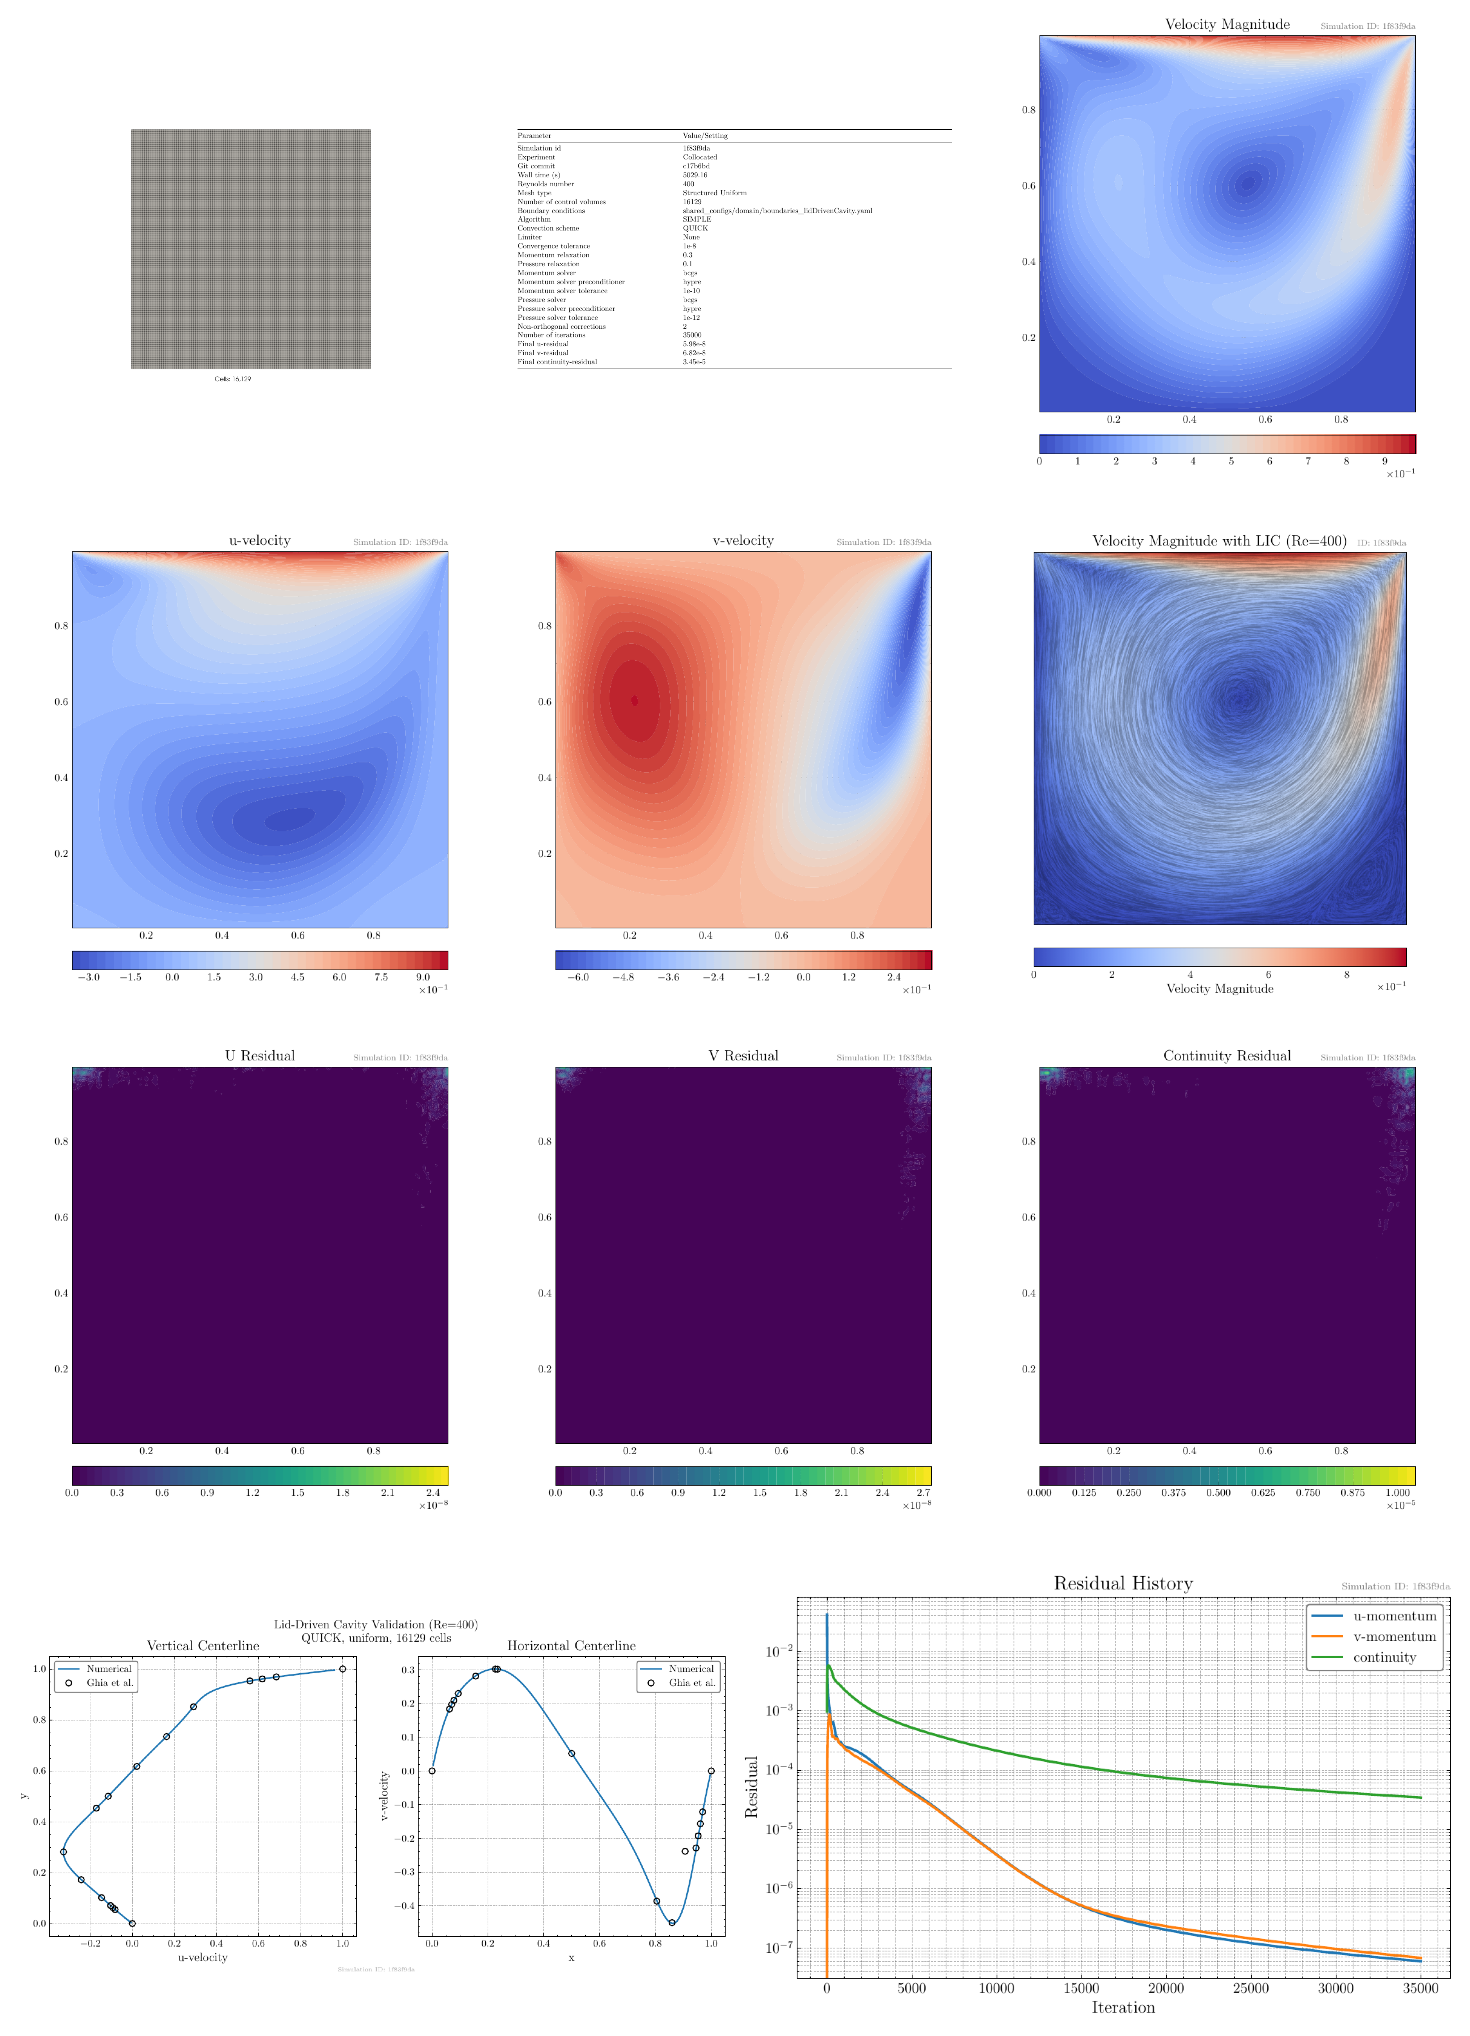
\includegraphics[width=0.85\linewidth]{AppendixPlots/lidDrivenCavity/Re_400/medium/lidDrivenCavity_Re400_uniform_medium_QUICK_1f83f9da.pdf}
    \caption{Liddrivencavity simulation at Re=400 using uniform medium mesh with QUICK discretization scheme (Simulation ID: 1f83f9da)}
    \label{sim.ldc.re400.unif.med.quick}
\end{figure}

\paragraph*{Uniform Mesh with TVD Scheme}
\addcontentsline{toc}{paragraph}{Uniform Mesh with TVD Scheme}
\label{para:liddrivencavity_re400_medium_uniform_TVD}

\begin{figure}[H]
    \centering
    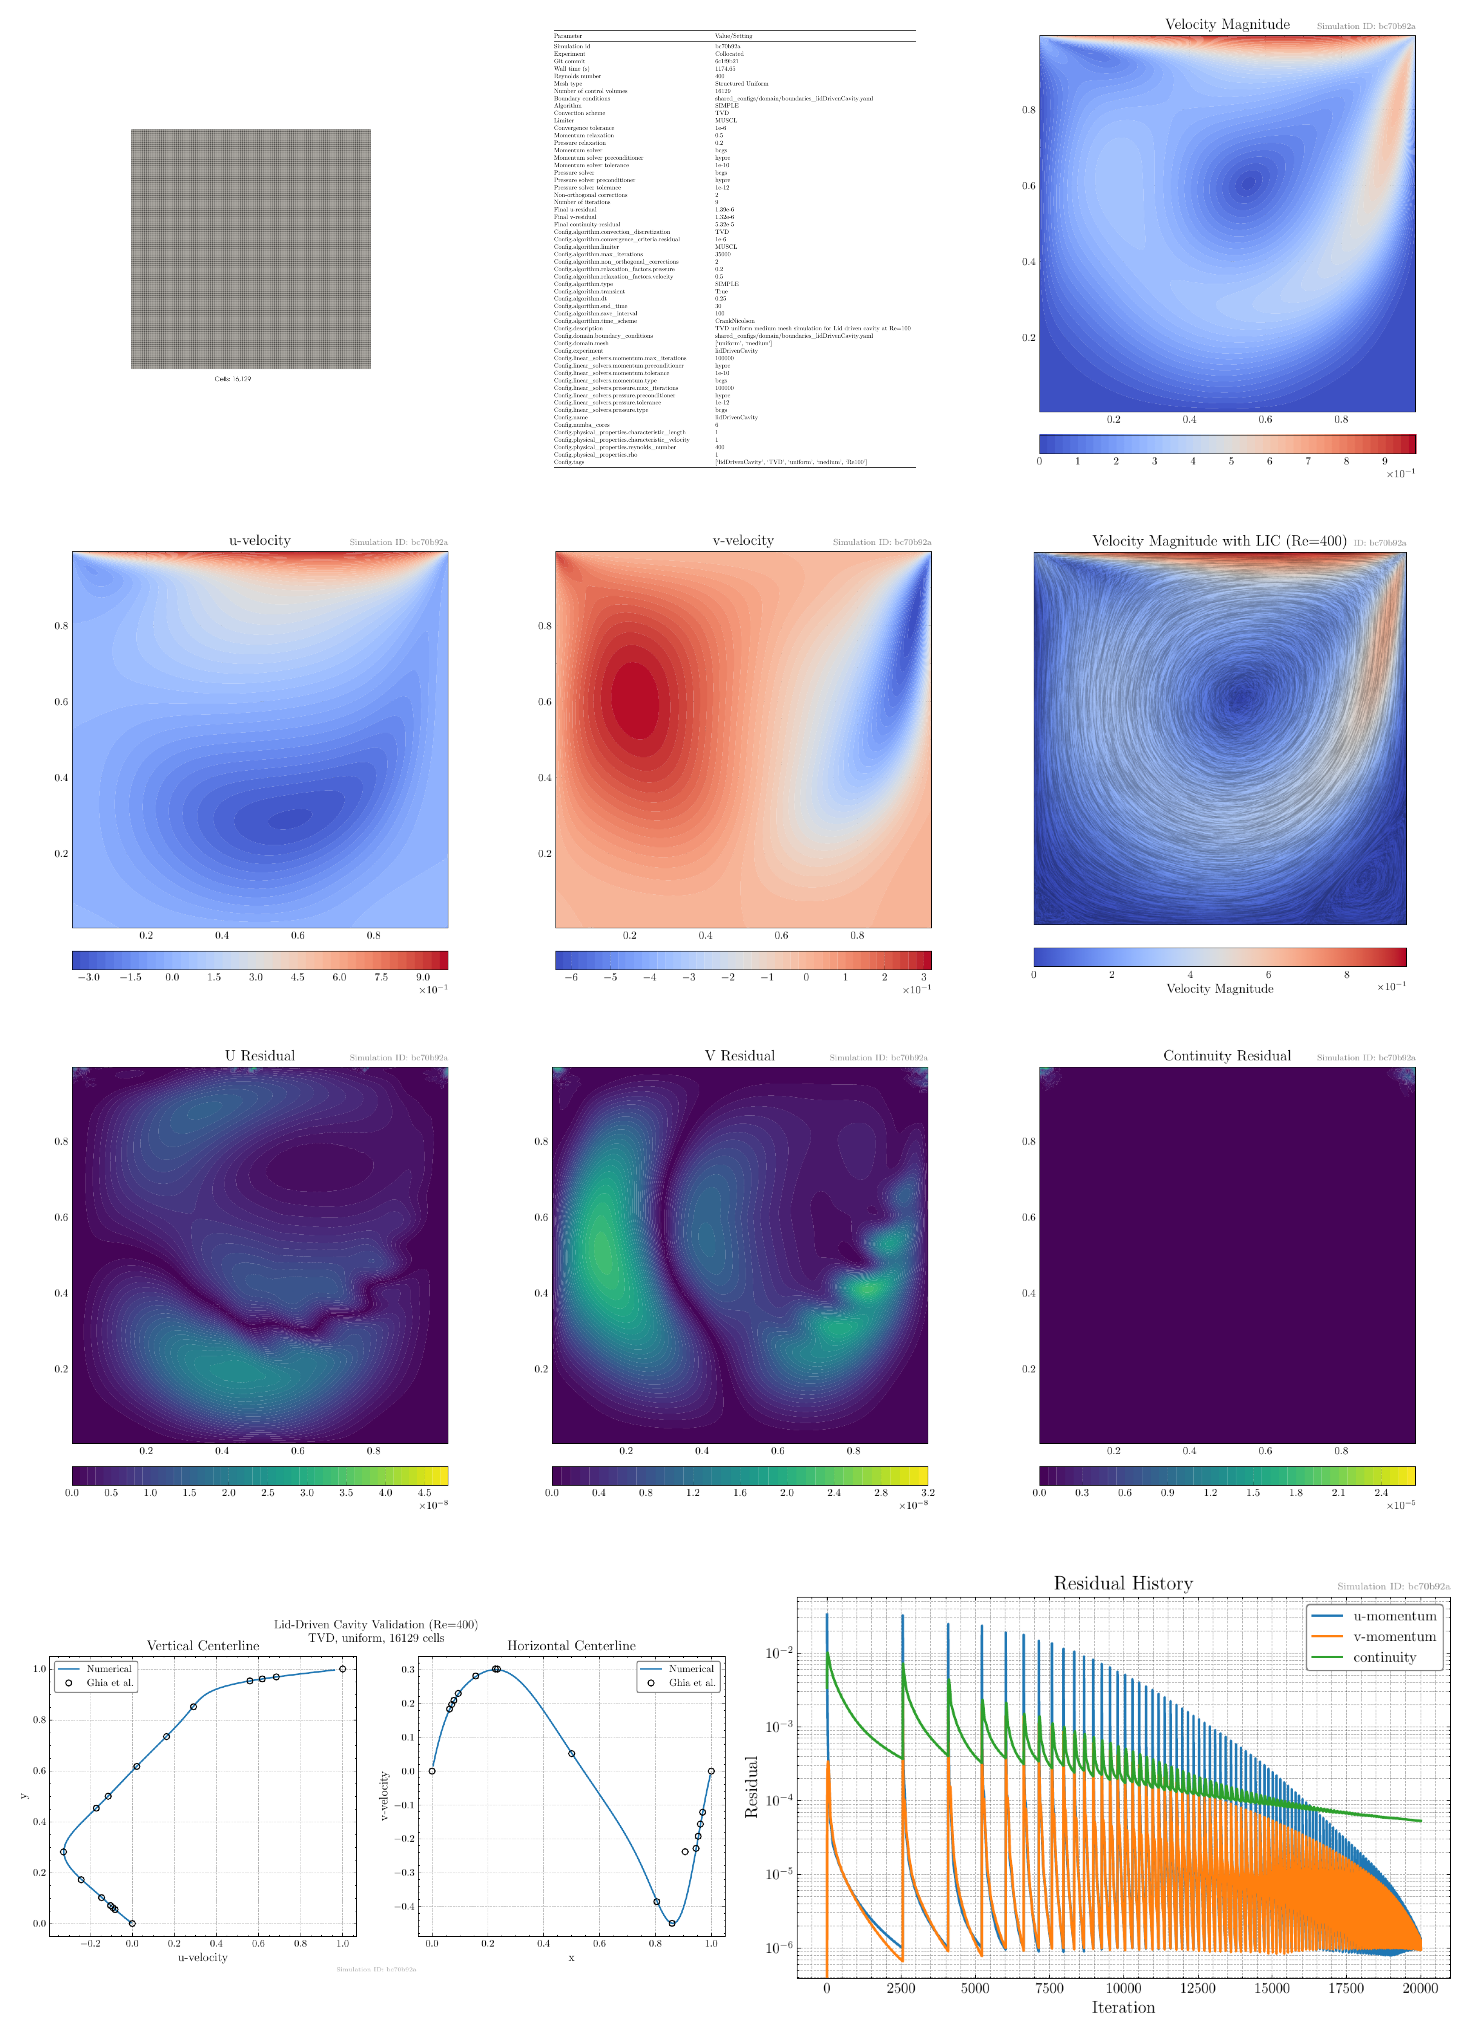
\includegraphics[width=0.85\linewidth]{AppendixPlots/lidDrivenCavity/Re_400/medium/lidDrivenCavity_Re400_uniform_medium_TVD_bc70b92a.pdf}
    \caption{Liddrivencavity simulation at Re=400 using uniform medium mesh with TVD discretization scheme (Simulation ID: bc70b92a)}
    \label{sim.ldc.re400.unif.med.tvd}
\end{figure}

\begin{figure}[H]
    \centering
    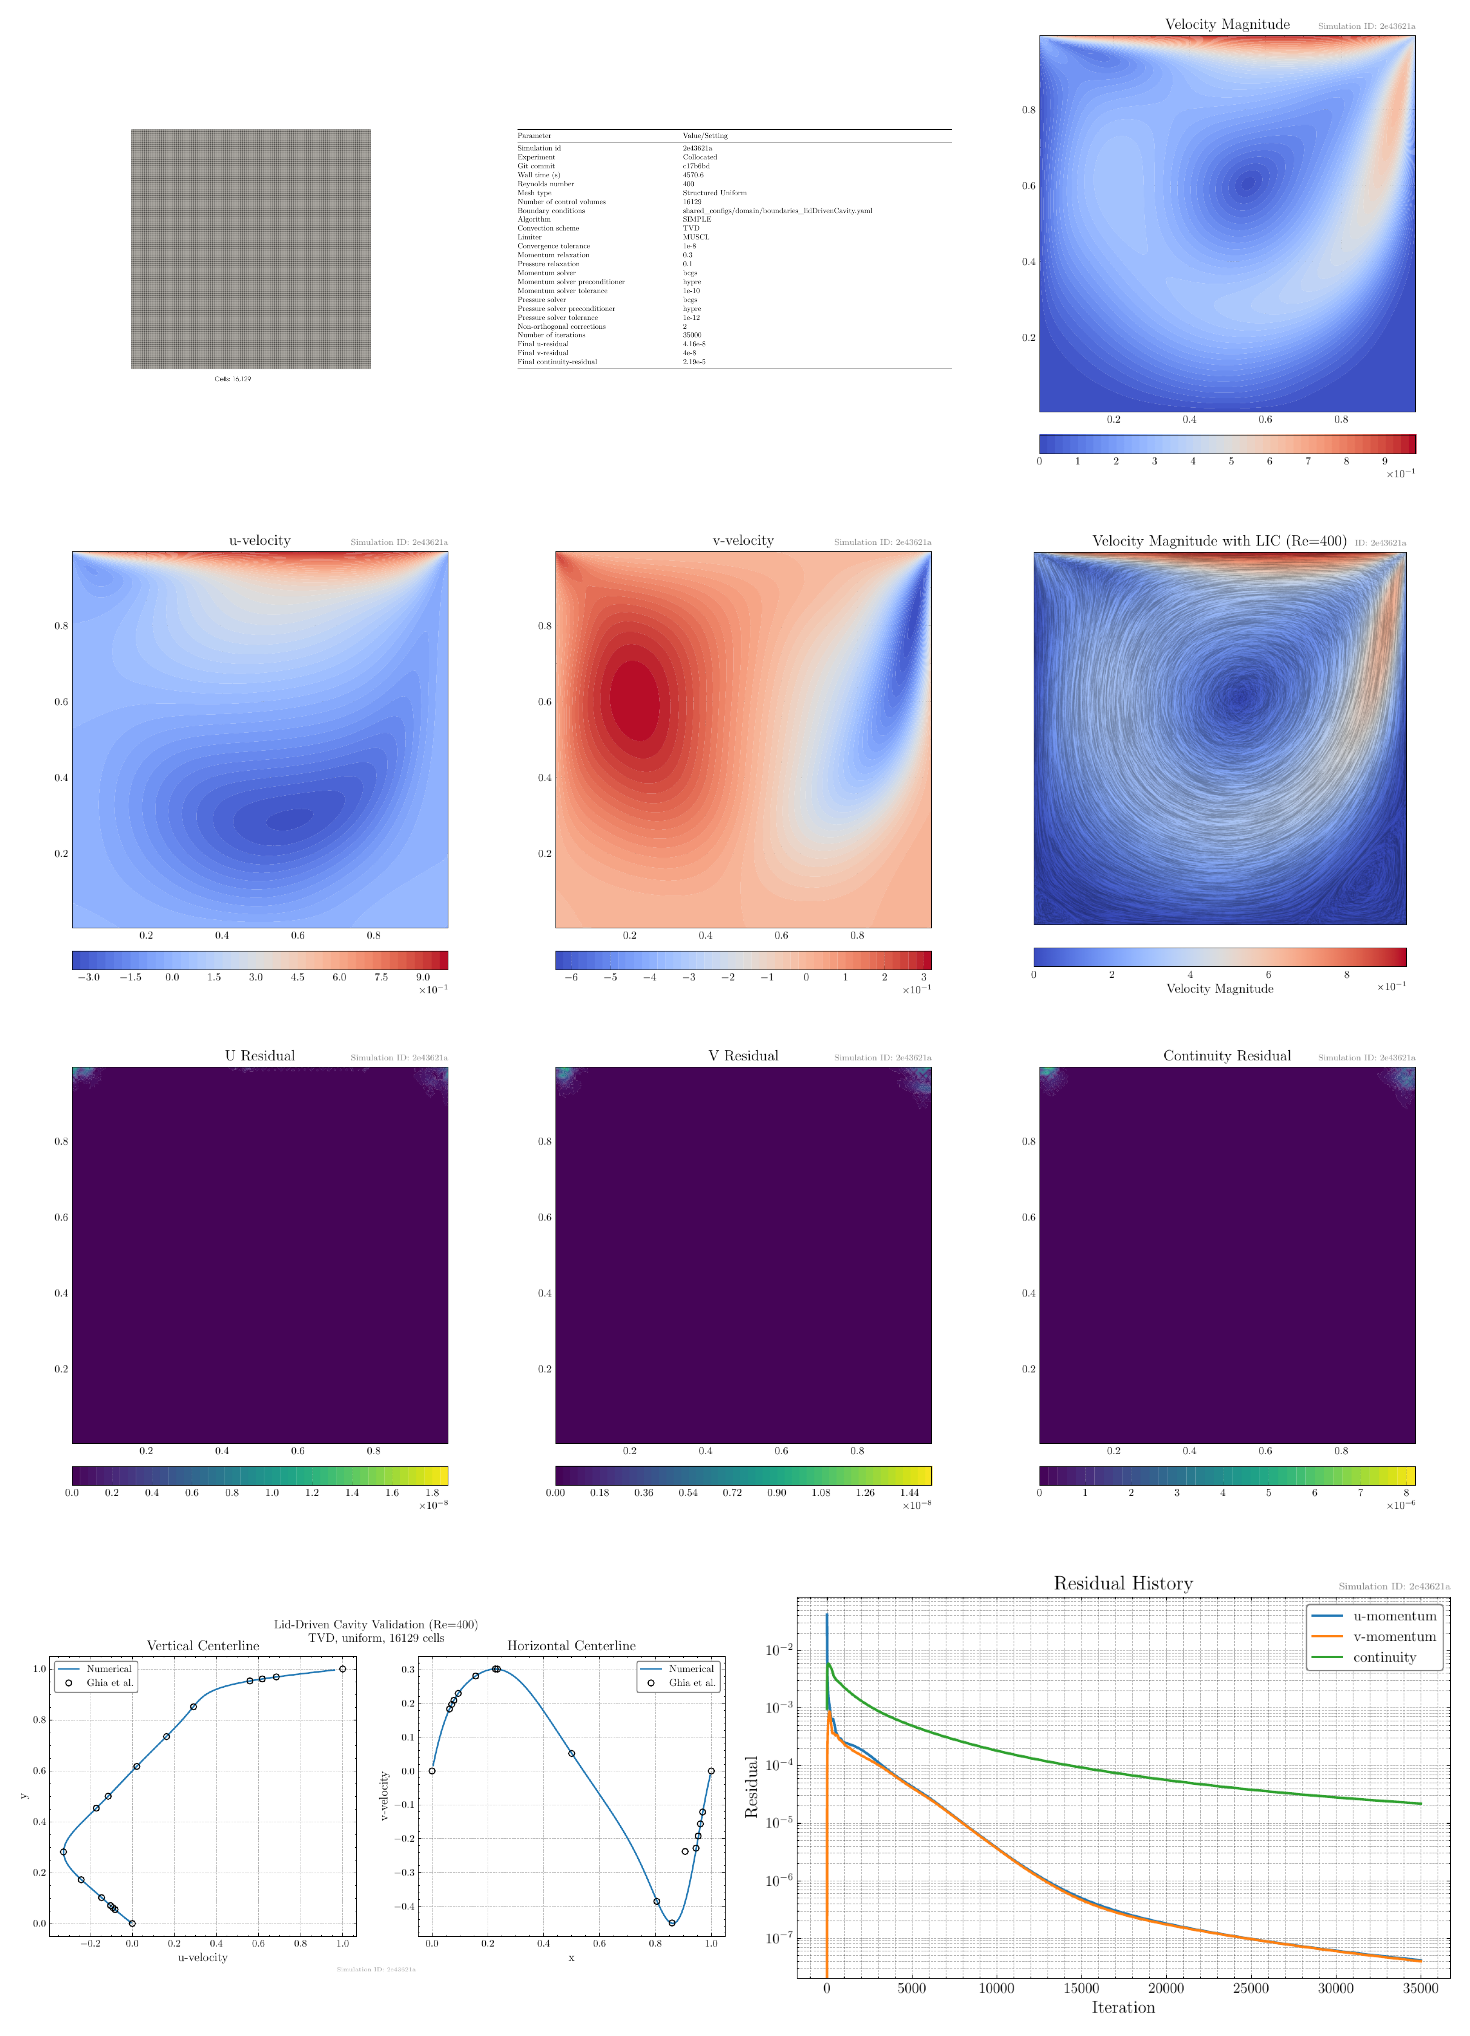
\includegraphics[width=0.85\linewidth]{AppendixPlots/lidDrivenCavity/Re_400/medium/lidDrivenCavity_Re400_uniform_medium_TVD_2e43621a.pdf}
    \caption{Liddrivencavity simulation at Re=400 using uniform medium mesh with TVD discretization scheme (Simulation ID: 2e43621a)}
    \label{sim.ldc.re400.unif.med.tvd}
\end{figure}

\paragraph*{Uniform Mesh with Upwind Scheme}
\addcontentsline{toc}{paragraph}{Uniform Mesh with Upwind Scheme}
\label{para:liddrivencavity_re400_medium_uniform_Upwind}

\begin{figure}[H]
    \centering
    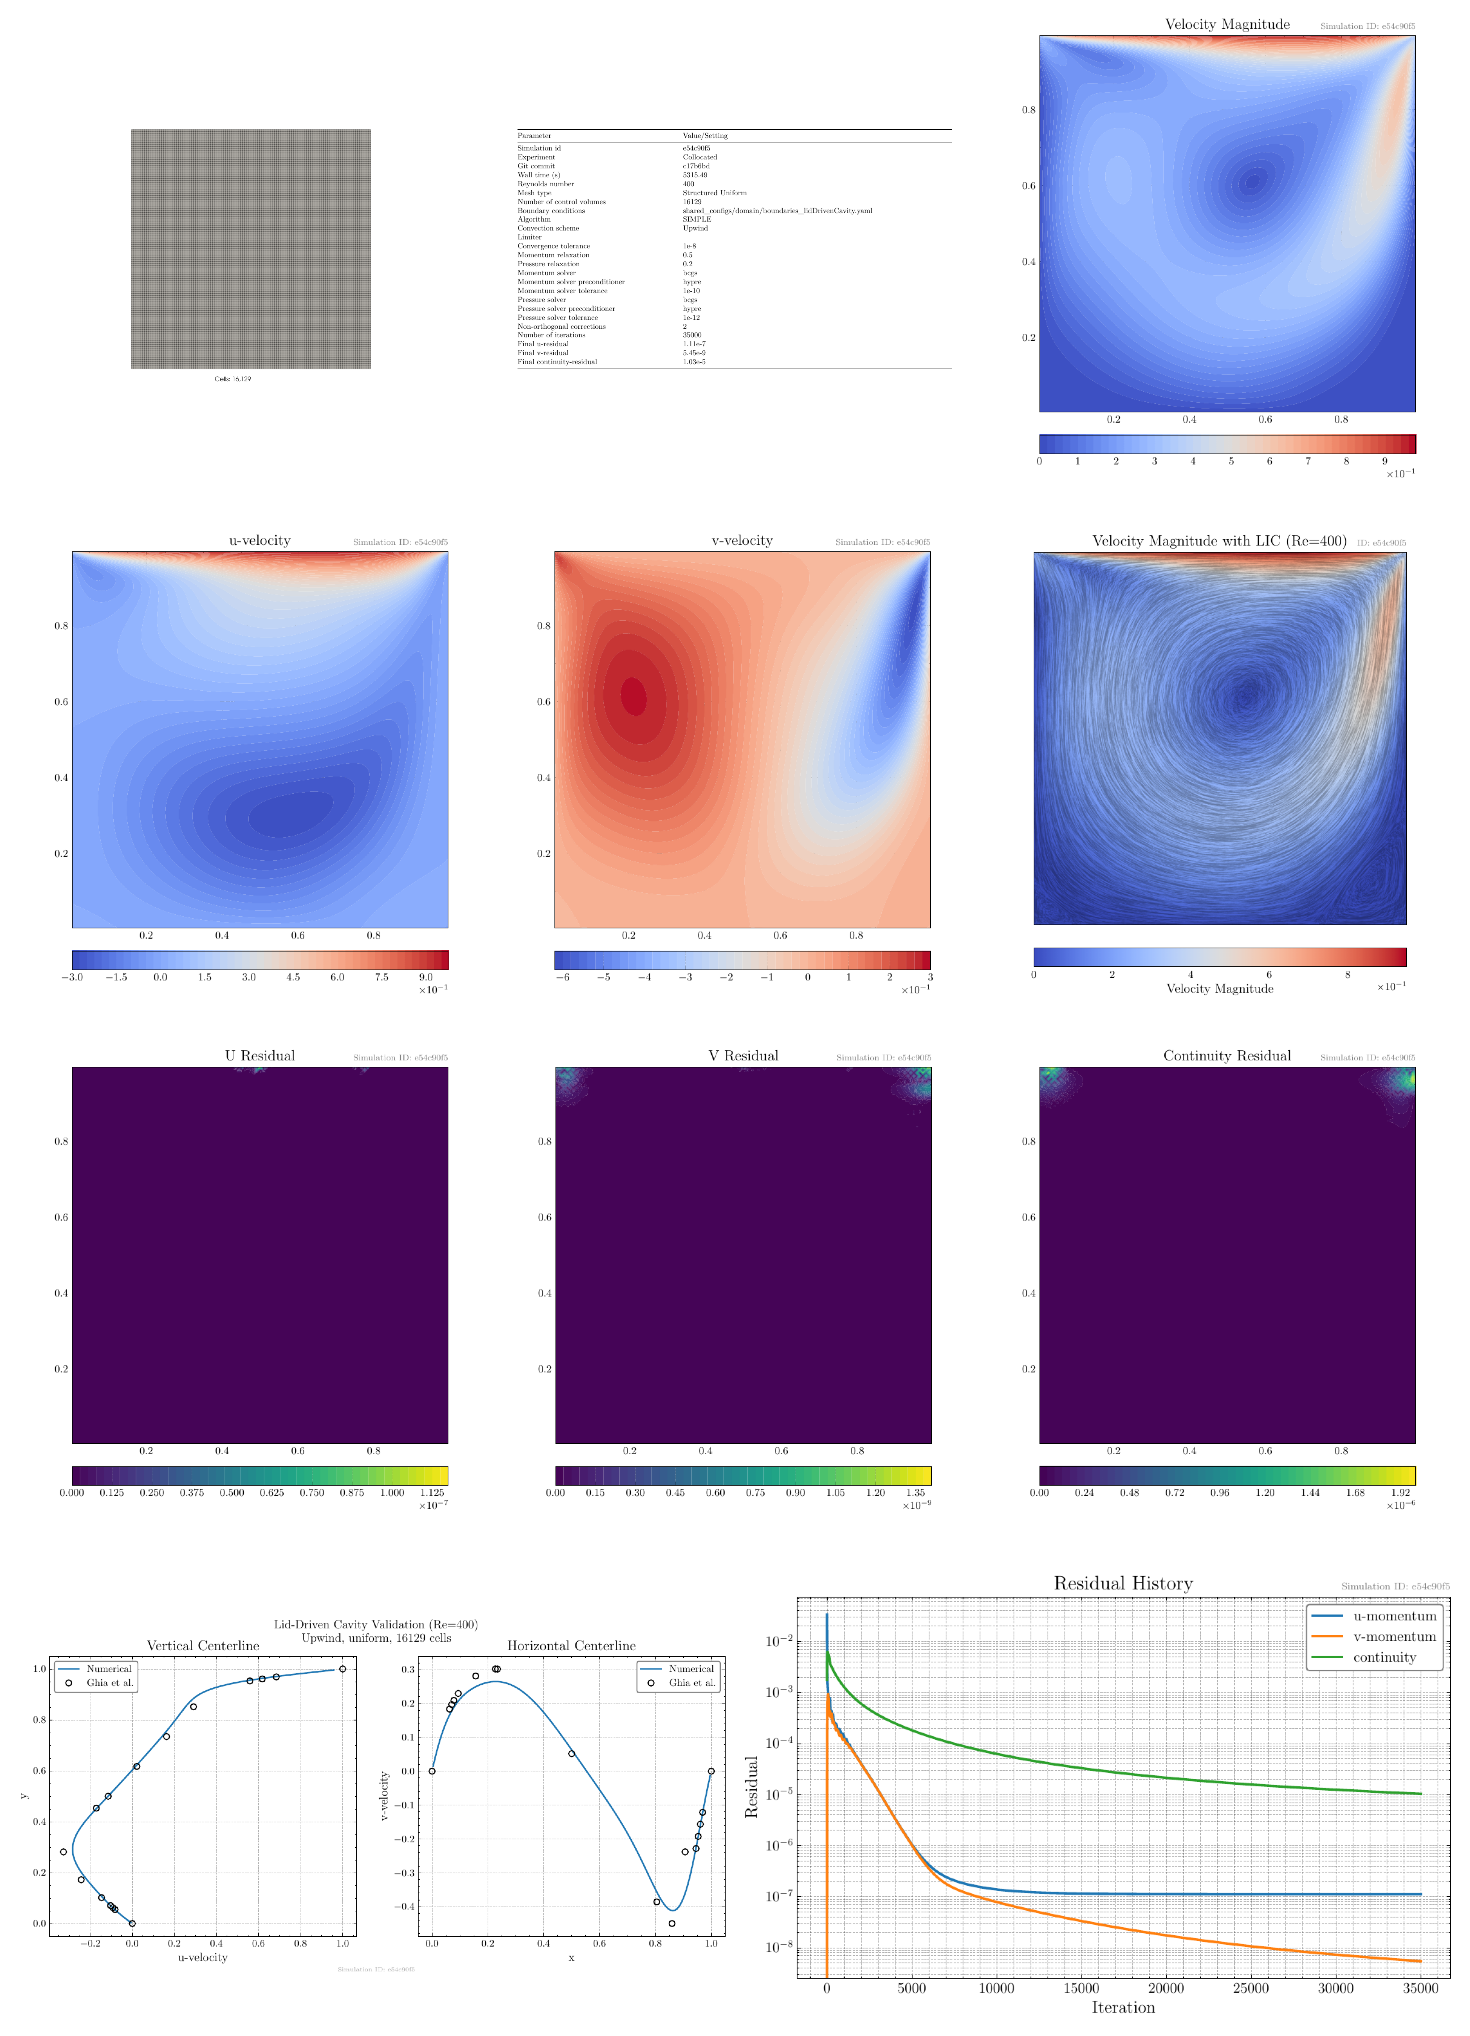
\includegraphics[width=0.85\linewidth]{AppendixPlots/lidDrivenCavity/Re_400/medium/lidDrivenCavity_Re400_uniform_medium_Upwind_e54c90f5.pdf}
    \caption{Liddrivencavity simulation at Re=400 using uniform medium mesh with Upwind discretization scheme (Simulation ID: e54c90f5)}
    \label{sim.ldc.re400.unif.med.upwind}
\end{figure}

\paragraph*{Unstructured Mesh with TVD Scheme}
\addcontentsline{toc}{paragraph}{Unstructured Mesh with TVD Scheme}
\label{para:liddrivencavity_re400_medium_unstructured_TVD}

\begin{figure}[H]
    \centering
    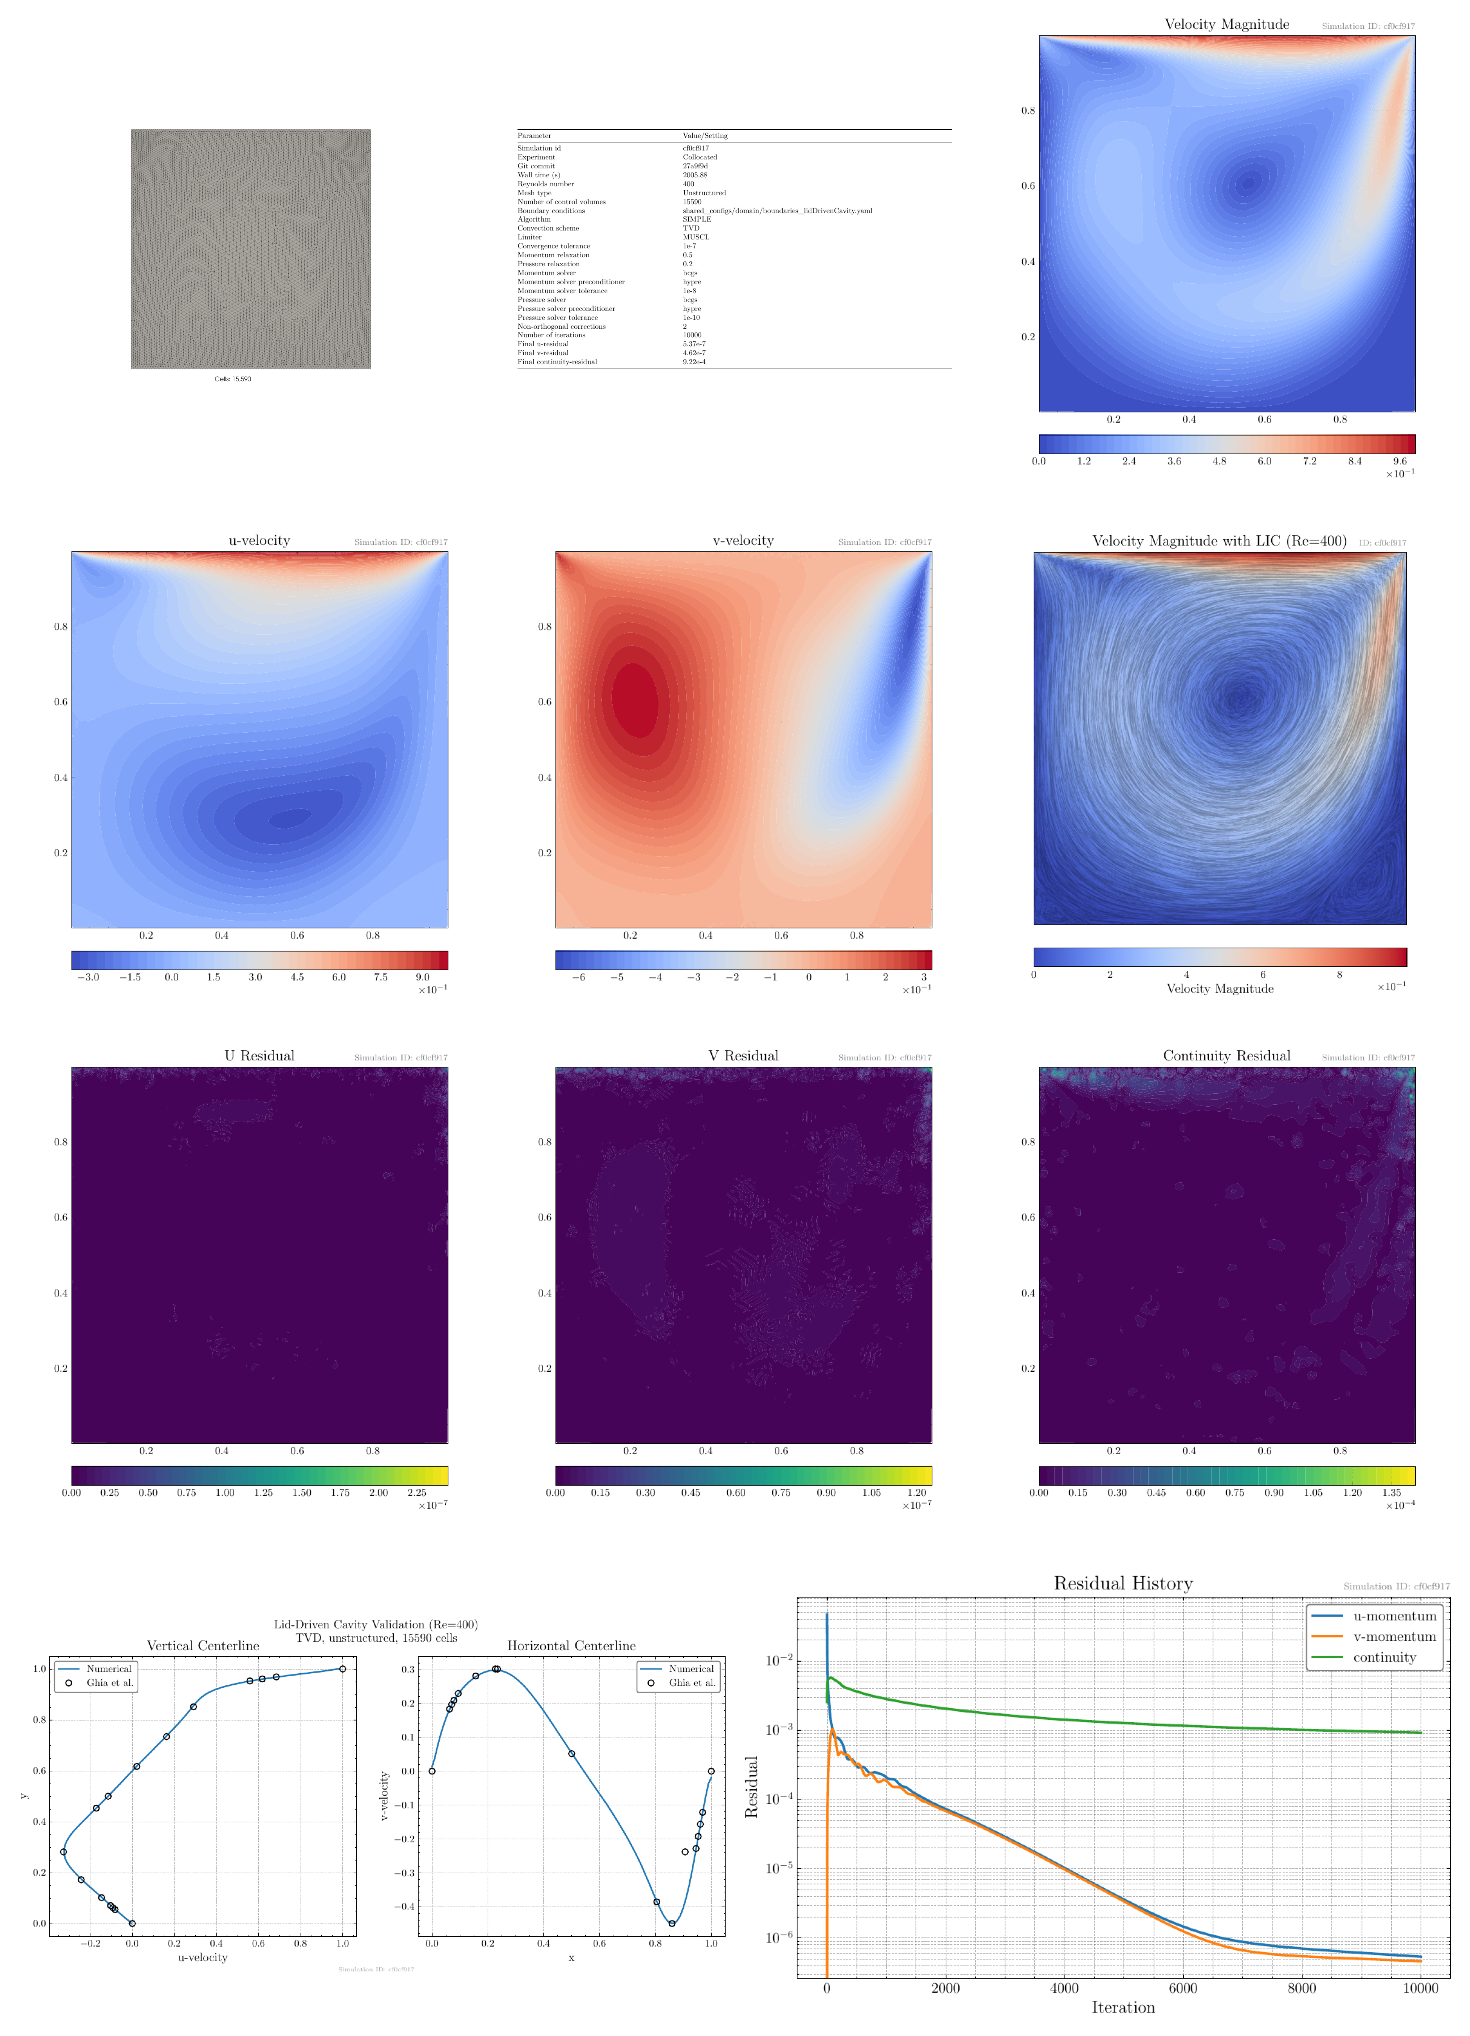
\includegraphics[width=0.85\linewidth]{AppendixPlots/lidDrivenCavity/Re_400/medium/lidDrivenCavity_Re400_unstructured_medium_TVD_cf0cf917.pdf}
    \caption{Liddrivencavity simulation at Re=400 using unstructured medium mesh with TVD discretization scheme (Simulation ID: cf0cf917)}
    \label{sim.ldc.re400.unstruct.med.tvd}
\end{figure}

\paragraph*{Unstructured Mesh with Upwind Scheme}
\addcontentsline{toc}{paragraph}{Unstructured Mesh with Upwind Scheme}
\label{para:liddrivencavity_re400_medium_unstructured_Upwind}

\begin{figure}[H]
    \centering
    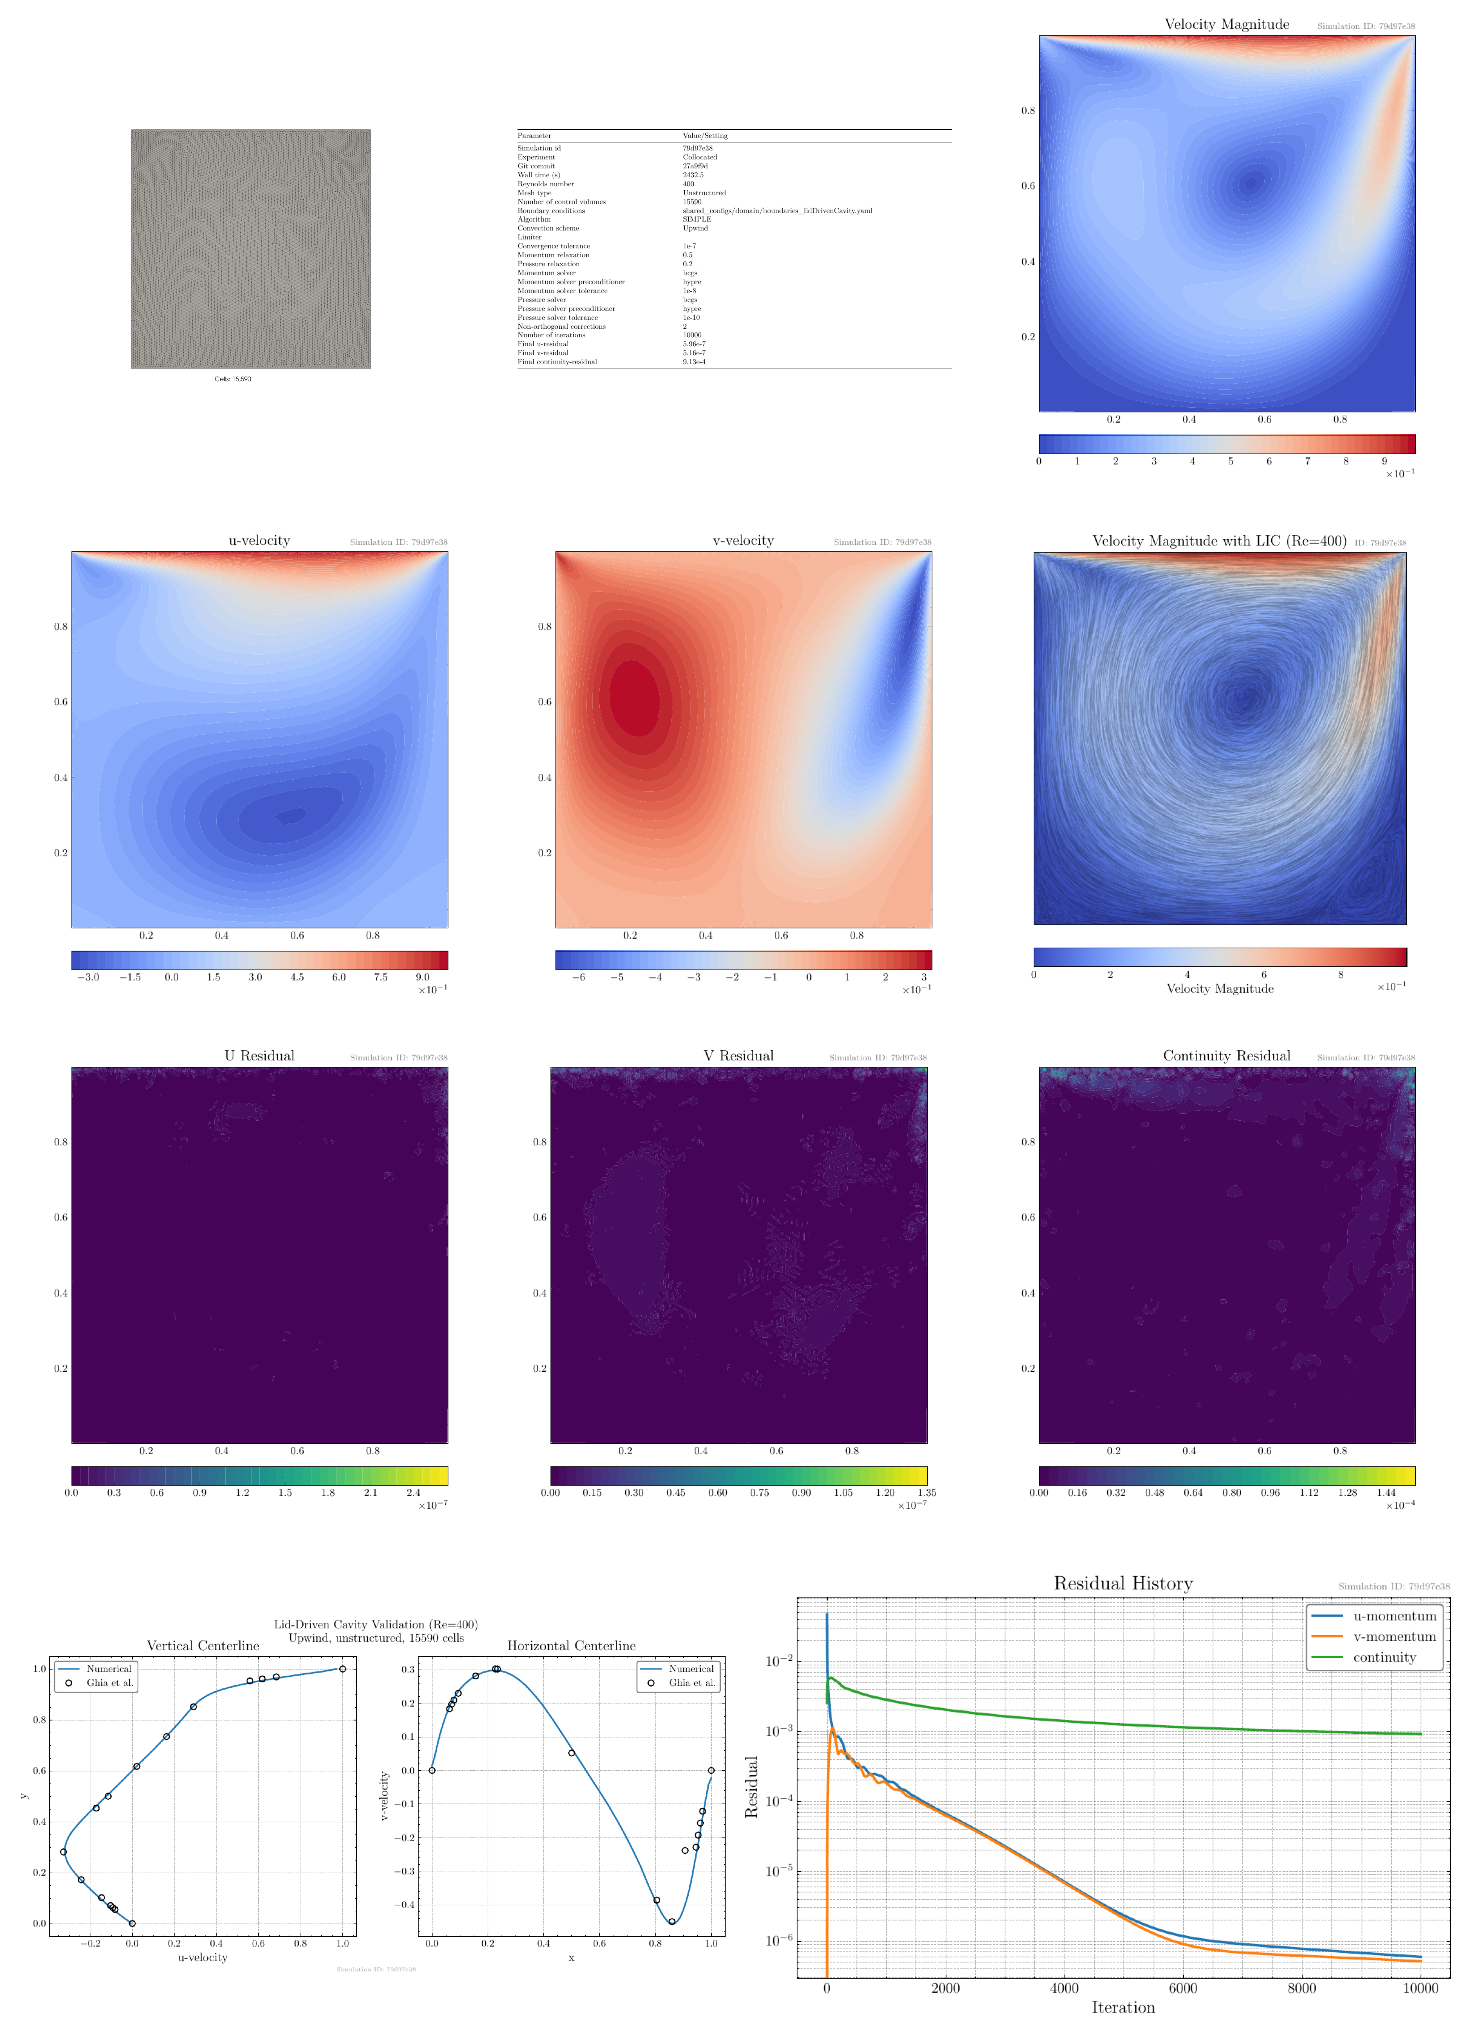
\includegraphics[width=0.85\linewidth]{AppendixPlots/lidDrivenCavity/Re_400/medium/lidDrivenCavity_Re400_unstructured_medium_Upwind_79d97e38.pdf}
    \caption{Liddrivencavity simulation at Re=400 using unstructured medium mesh with Upwind discretization scheme (Simulation ID: 79d97e38)}
    \label{sim.ldc.re400.unstruct.med.upwind}
\end{figure}

\clearpage

\subsubsection*{Fine Mesh}
\addcontentsline{toc}{subsubsection}{Fine Mesh}
\label{subsubsec:liddrivencavity_re400_fine}

\paragraph*{Uniform Mesh with TVD Scheme}
\addcontentsline{toc}{paragraph}{Uniform Mesh with TVD Scheme}
\label{para:liddrivencavity_re400_fine_uniform_TVD}

\begin{figure}[H]
    \centering
    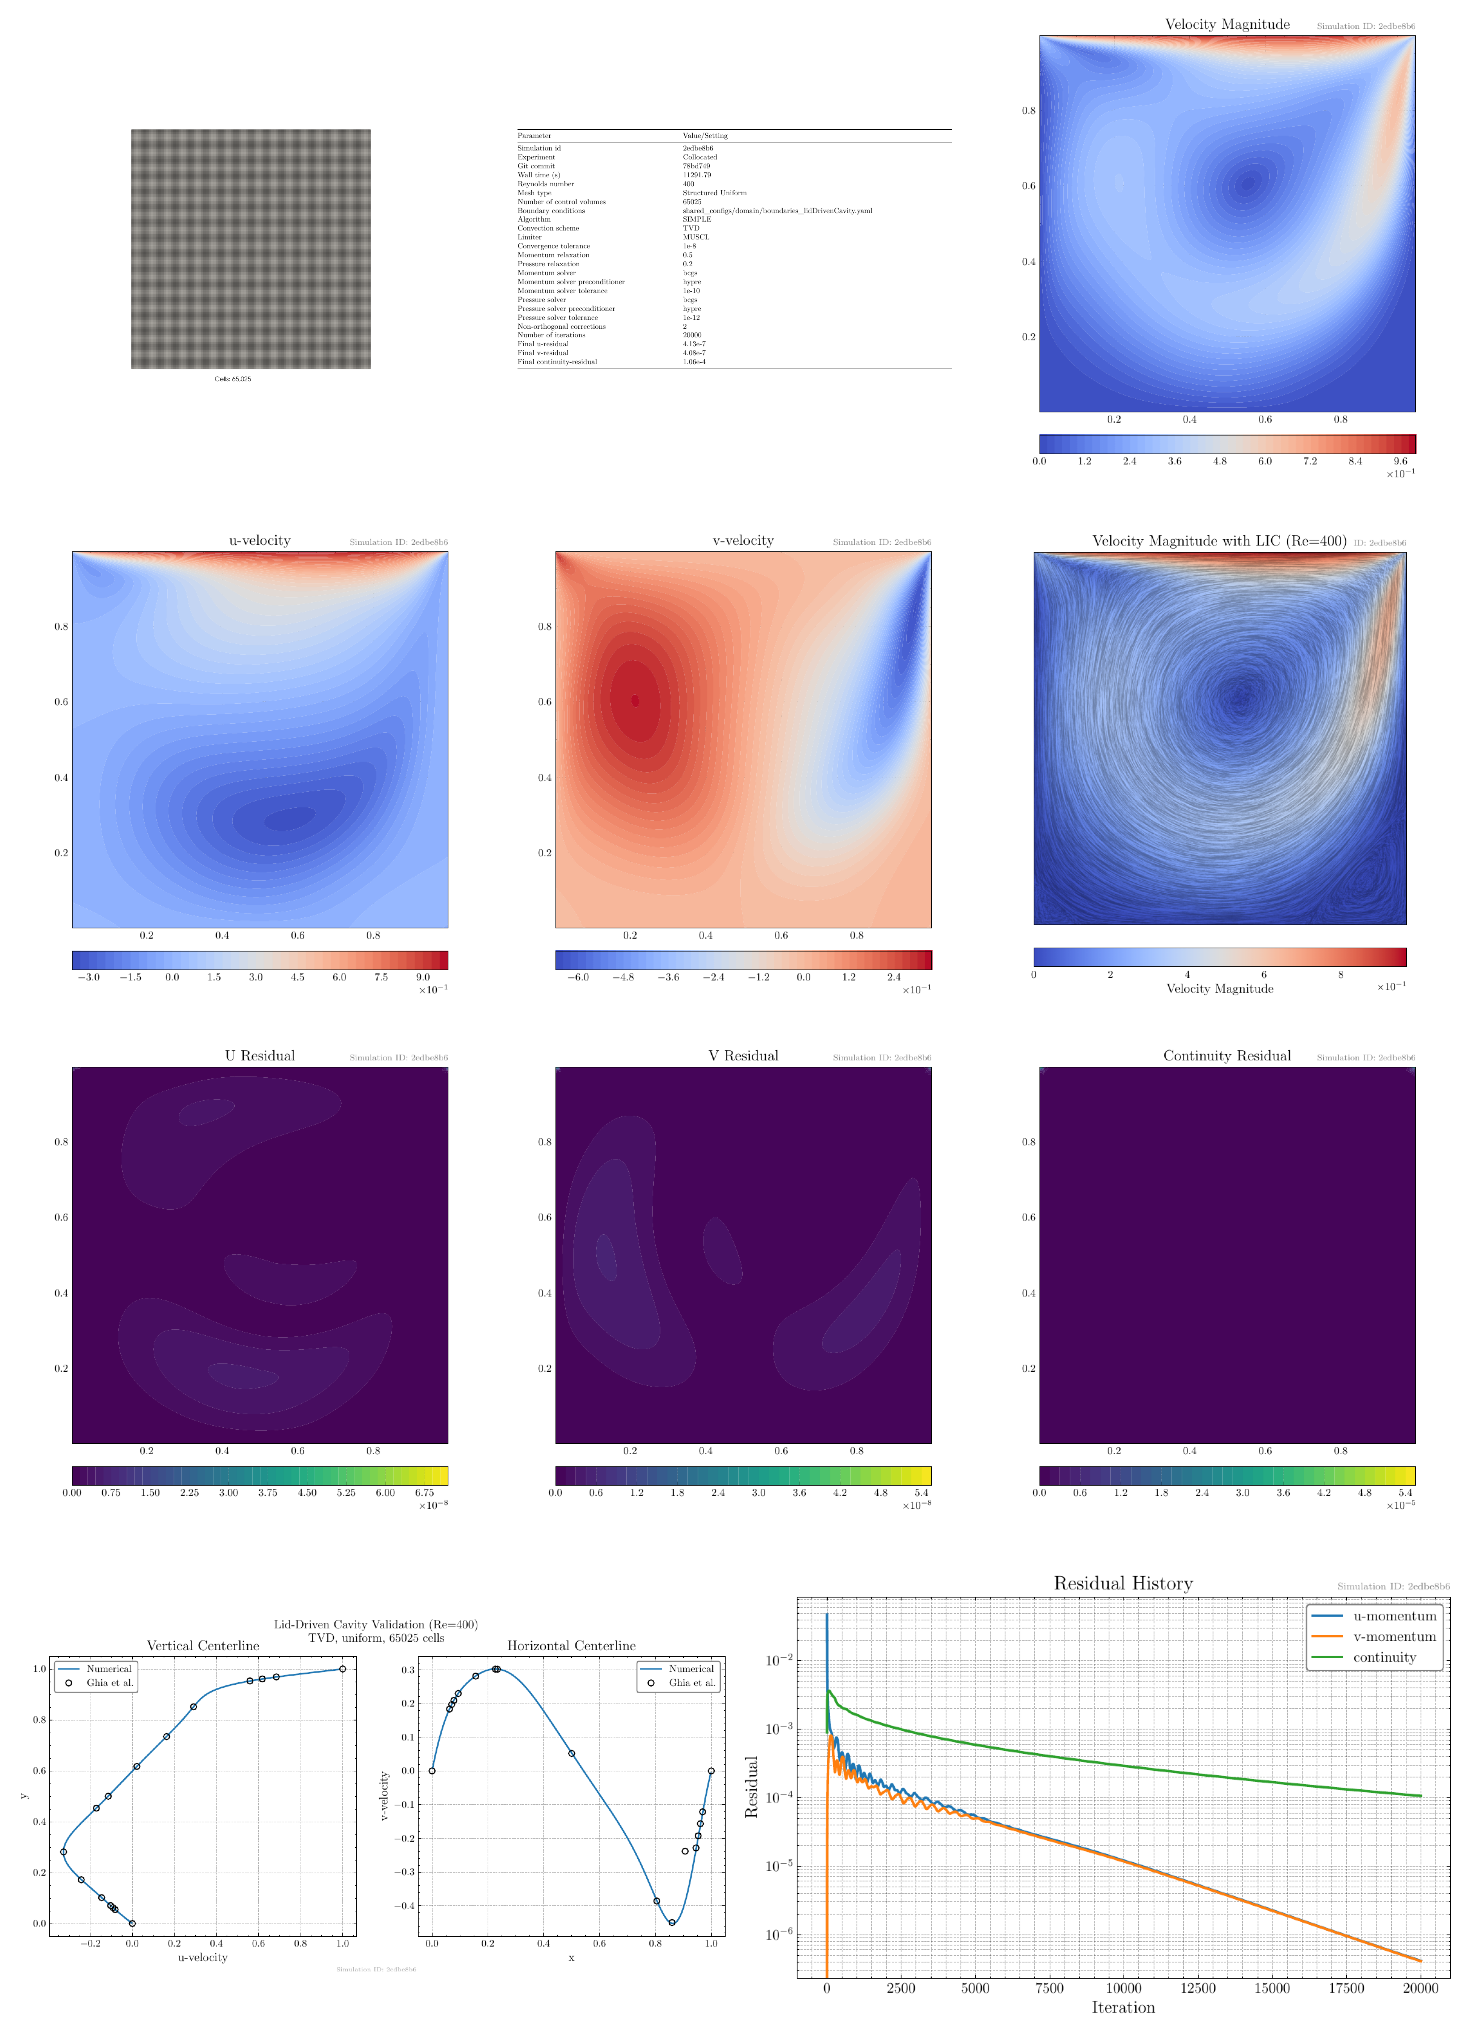
\includegraphics[width=0.85\linewidth]{AppendixPlots/lidDrivenCavity/Re_400/fine/lidDrivenCavity_Re400_uniform_fine_TVD_2edbe8b6.pdf}
    \caption{Liddrivencavity simulation at Re=400 using uniform fine mesh with TVD discretization scheme (Simulation ID: 2edbe8b6)}
    \label{sim.ldc.re400.unif.fine.tvd}
\end{figure}

\paragraph*{Uniform Mesh with Upwind Scheme}
\addcontentsline{toc}{paragraph}{Uniform Mesh with Upwind Scheme}
\label{para:liddrivencavity_re400_fine_uniform_Upwind}

\begin{figure}[H]
    \centering
    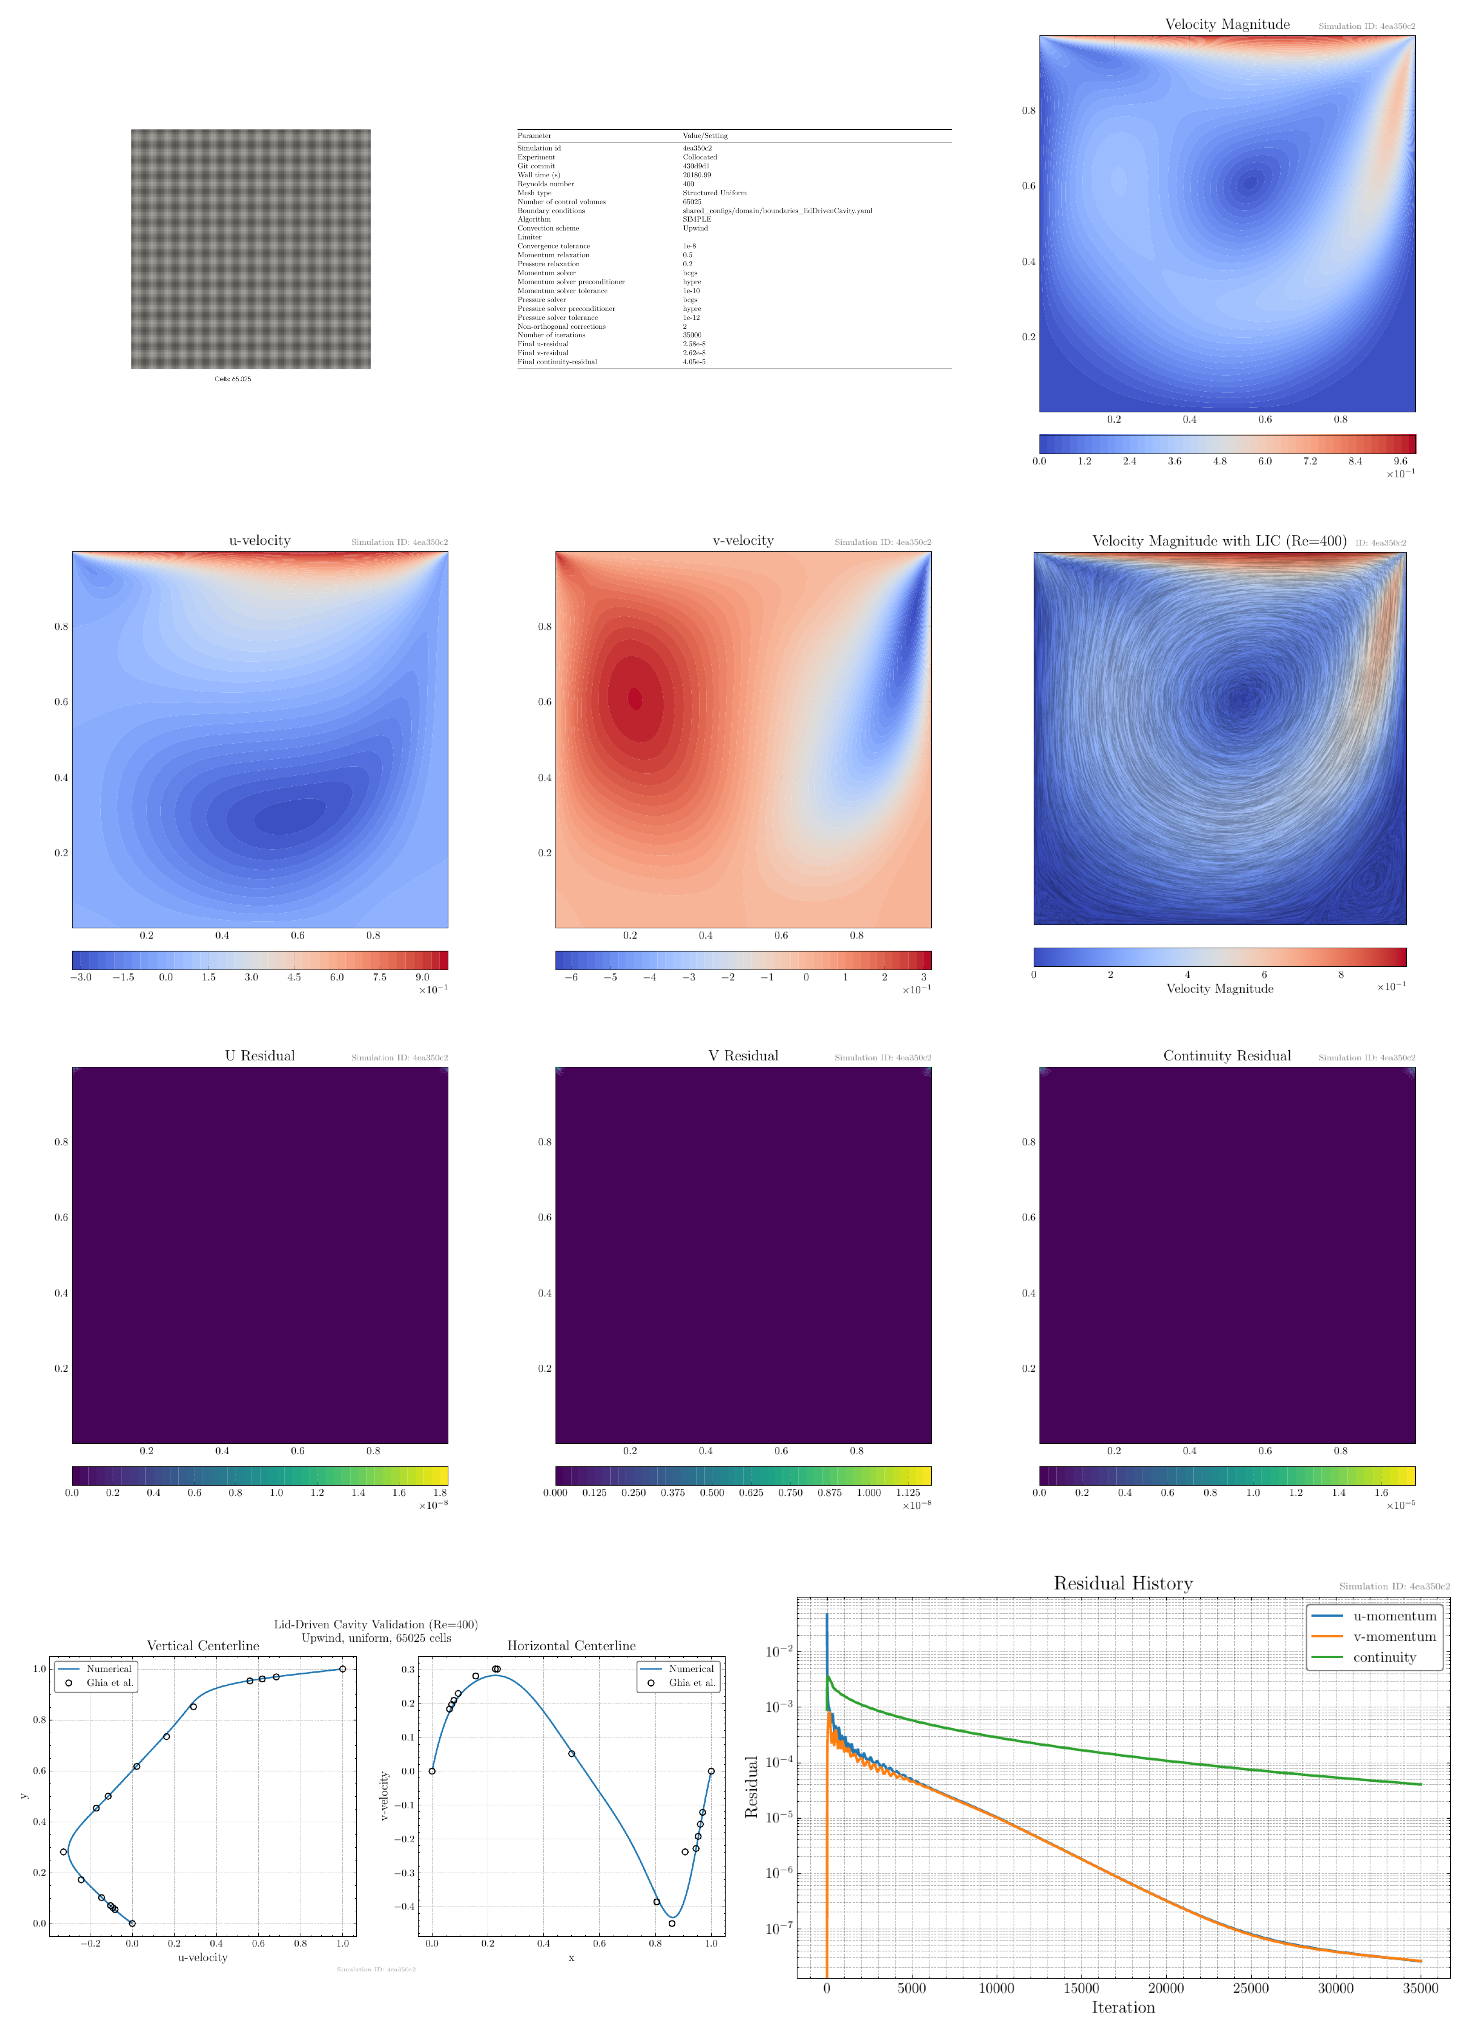
\includegraphics[width=0.85\linewidth]{AppendixPlots/lidDrivenCavity/Re_400/fine/lidDrivenCavity_Re400_uniform_fine_Upwind_4ea350c2.pdf}
    \caption{Liddrivencavity simulation at Re=400 using uniform fine mesh with Upwind discretization scheme (Simulation ID: 4ea350c2)}
    \label{sim.ldc.re400.unif.fine.upwind}
\end{figure}

\paragraph*{Unstructured Mesh with TVD Scheme}
\addcontentsline{toc}{paragraph}{Unstructured Mesh with TVD Scheme}
\label{para:liddrivencavity_re400_fine_unstructured_TVD}

\begin{figure}[H]
    \centering
    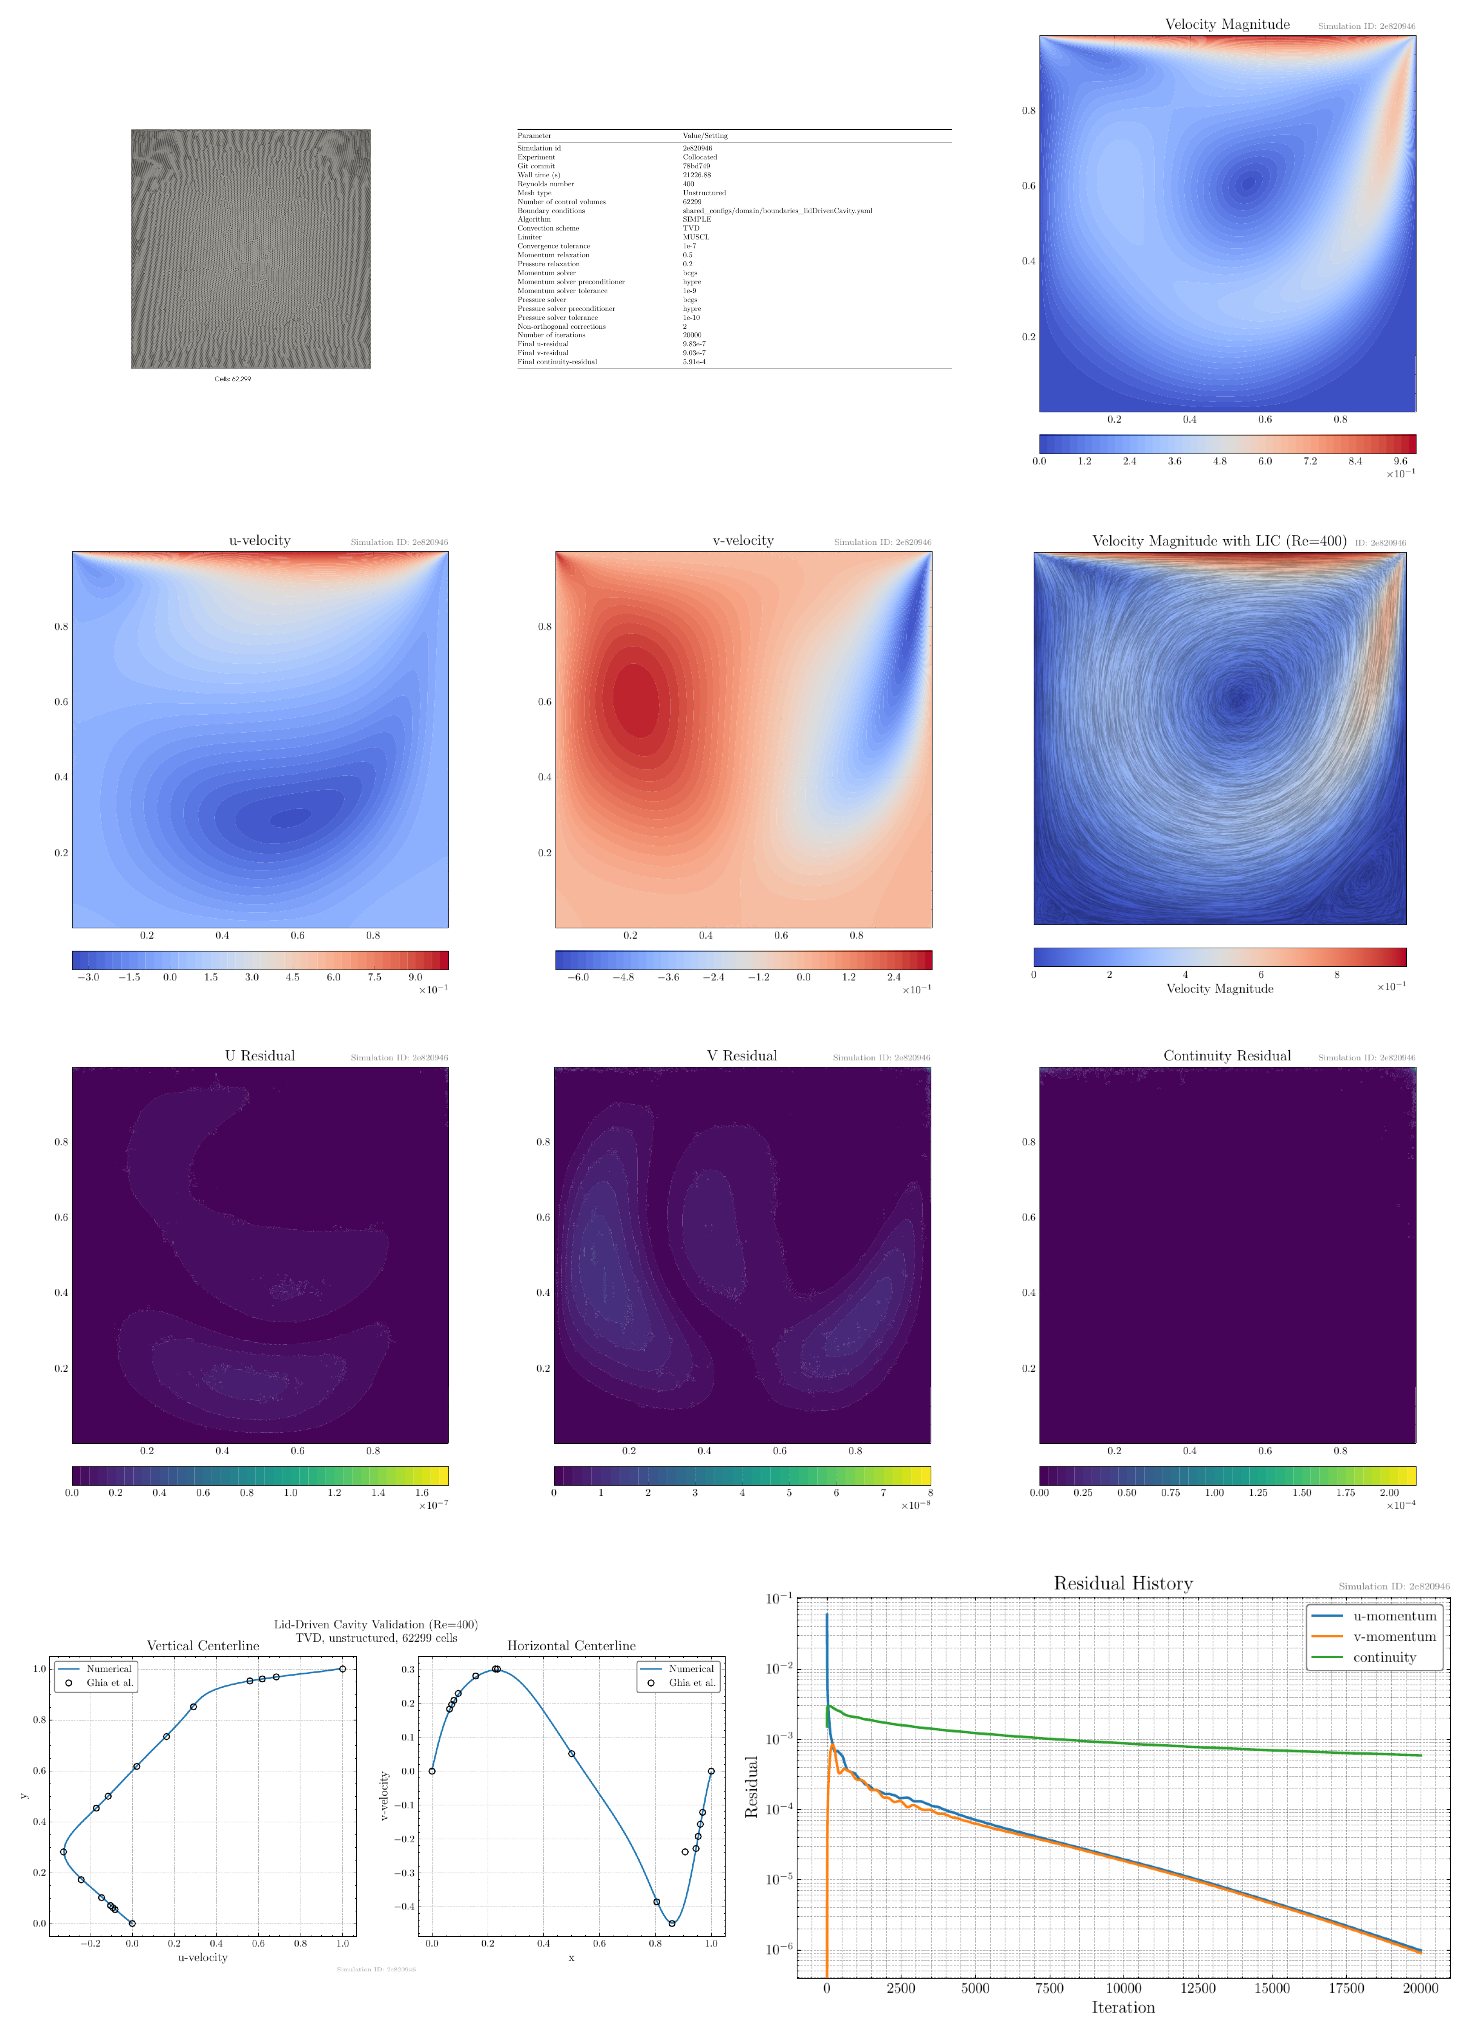
\includegraphics[width=0.85\linewidth]{AppendixPlots/lidDrivenCavity/Re_400/fine/lidDrivenCavity_Re400_unstructured_fine_TVD_2e820946.pdf}
    \caption{Liddrivencavity simulation at Re=400 using unstructured fine mesh with TVD discretization scheme (Simulation ID: 2e820946)}
    \label{sim.ldc.re400.unstruct.fine.tvd}
\end{figure}

\paragraph*{Unstructured Mesh with Upwind Scheme}
\addcontentsline{toc}{paragraph}{Unstructured Mesh with Upwind Scheme}
\label{para:liddrivencavity_re400_fine_unstructured_Upwind}

\begin{figure}[H]
    \centering
    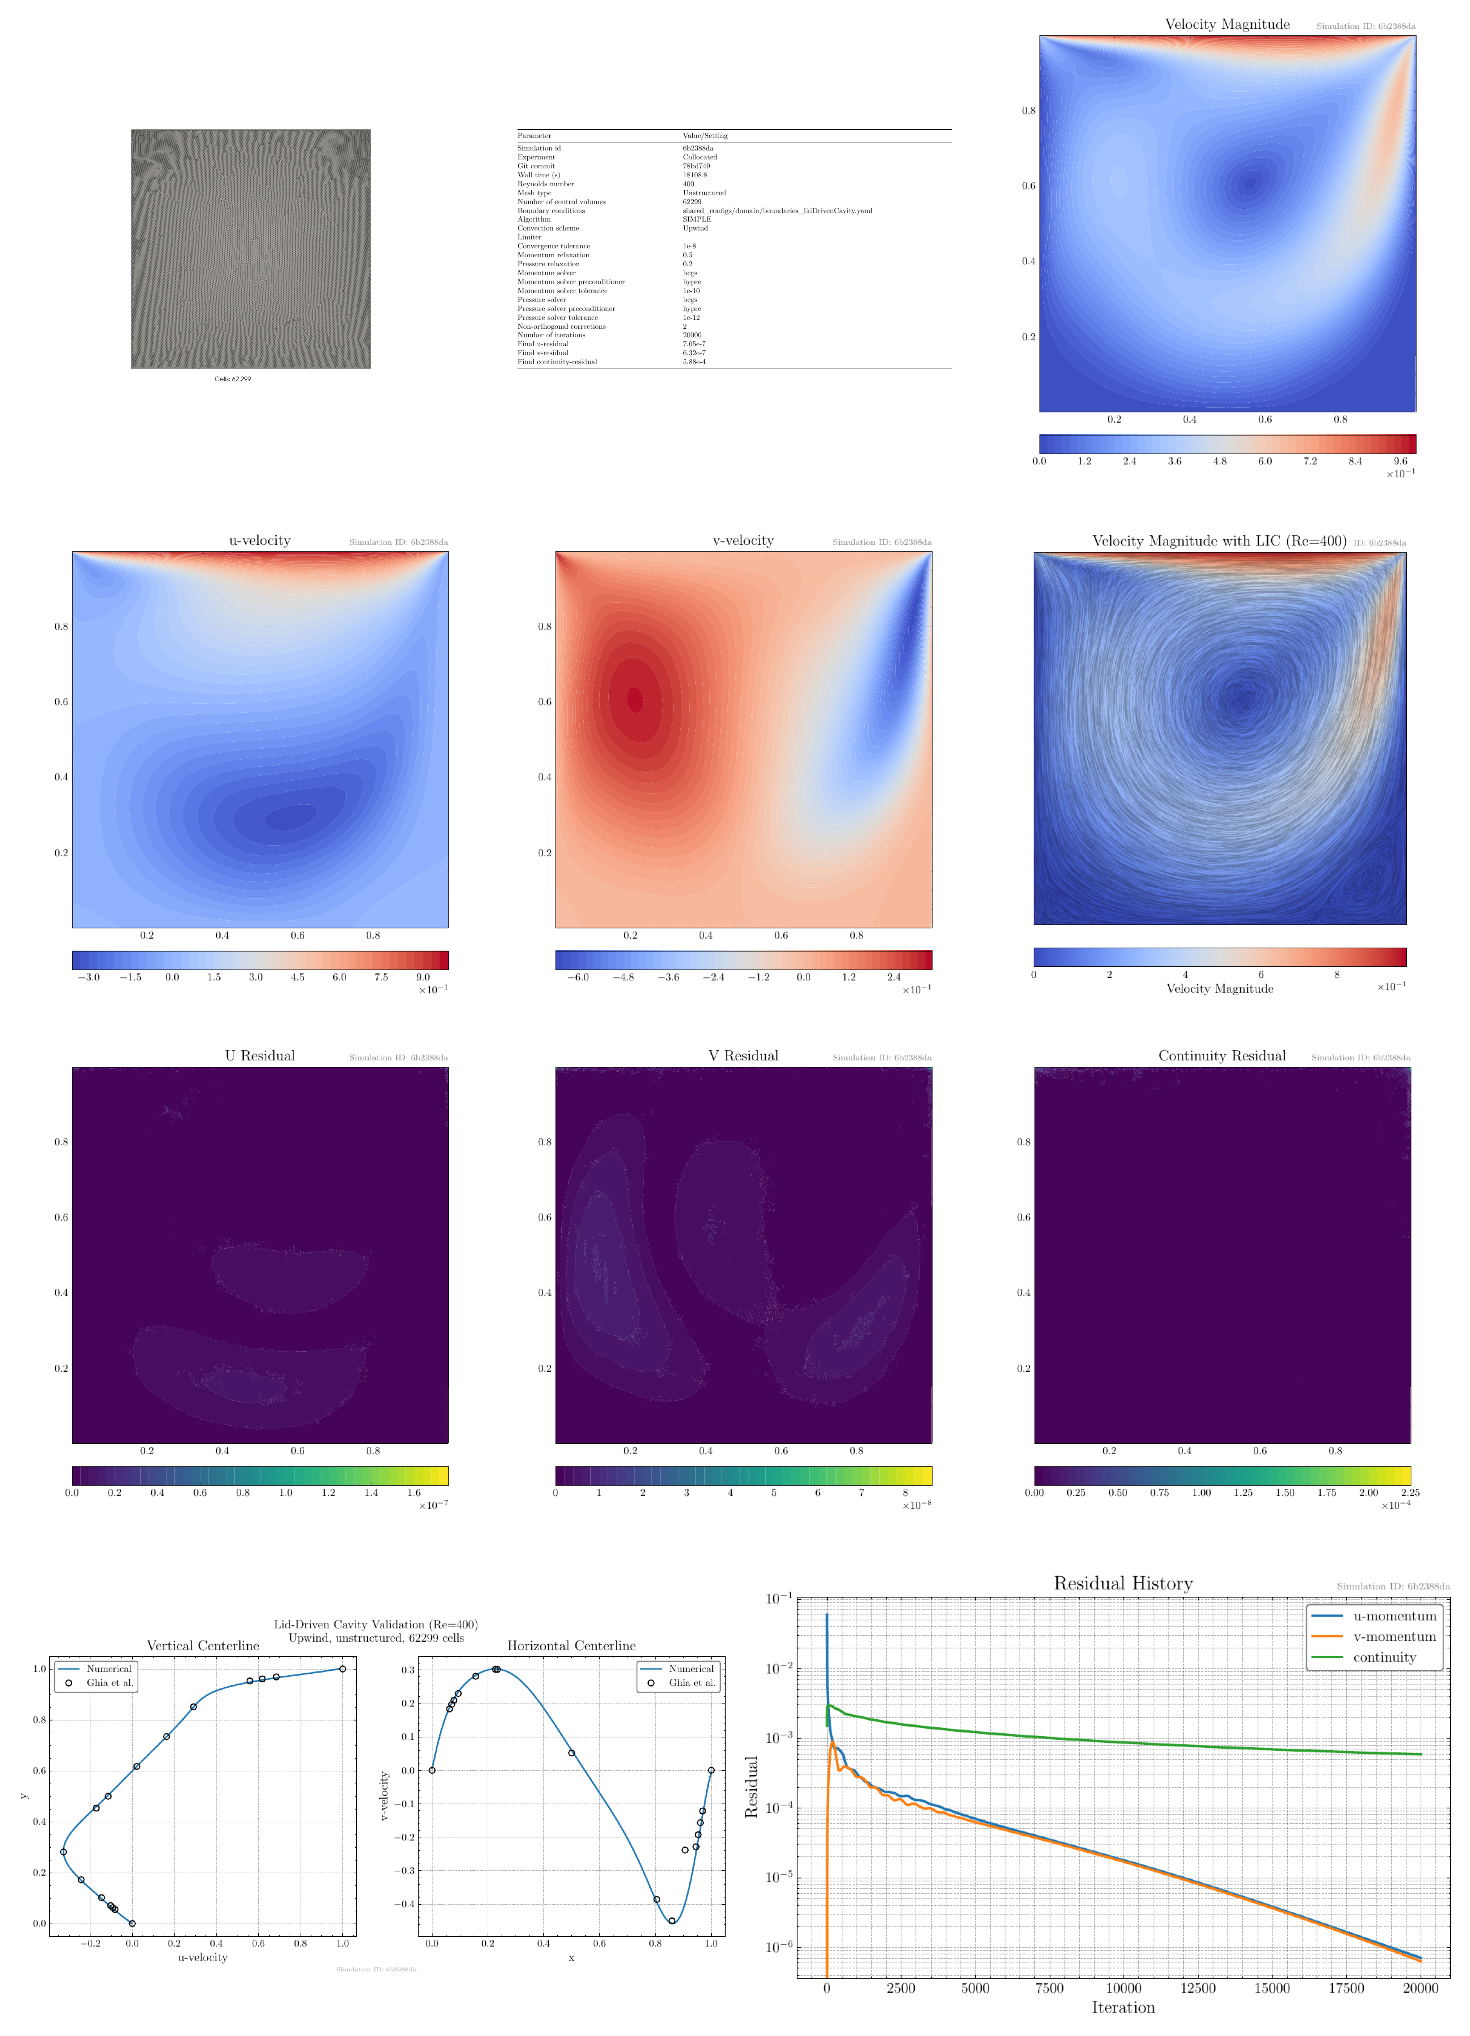
\includegraphics[width=0.85\linewidth]{AppendixPlots/lidDrivenCavity/Re_400/fine/lidDrivenCavity_Re400_unstructured_fine_Upwind_6b2388da.pdf}
    \caption{Liddrivencavity simulation at Re=400 using unstructured fine mesh with Upwind discretization scheme (Simulation ID: 6b2388da)}
    \label{sim.ldc.re400.unstruct.fine.upwind}
\end{figure}

\clearpage

\subsubsection*{127X127 Mesh}
\addcontentsline{toc}{subsubsection}{127X127 Mesh}
\label{subsubsec:liddrivencavity_re400_127x127}

\paragraph*{Structured Mesh with Power Law Scheme}
\addcontentsline{toc}{paragraph}{Structured Mesh with Power Law Scheme}
\label{para:liddrivencavity_re400_127x127_structured_Power Law}

\begin{figure}[H]
    \centering
    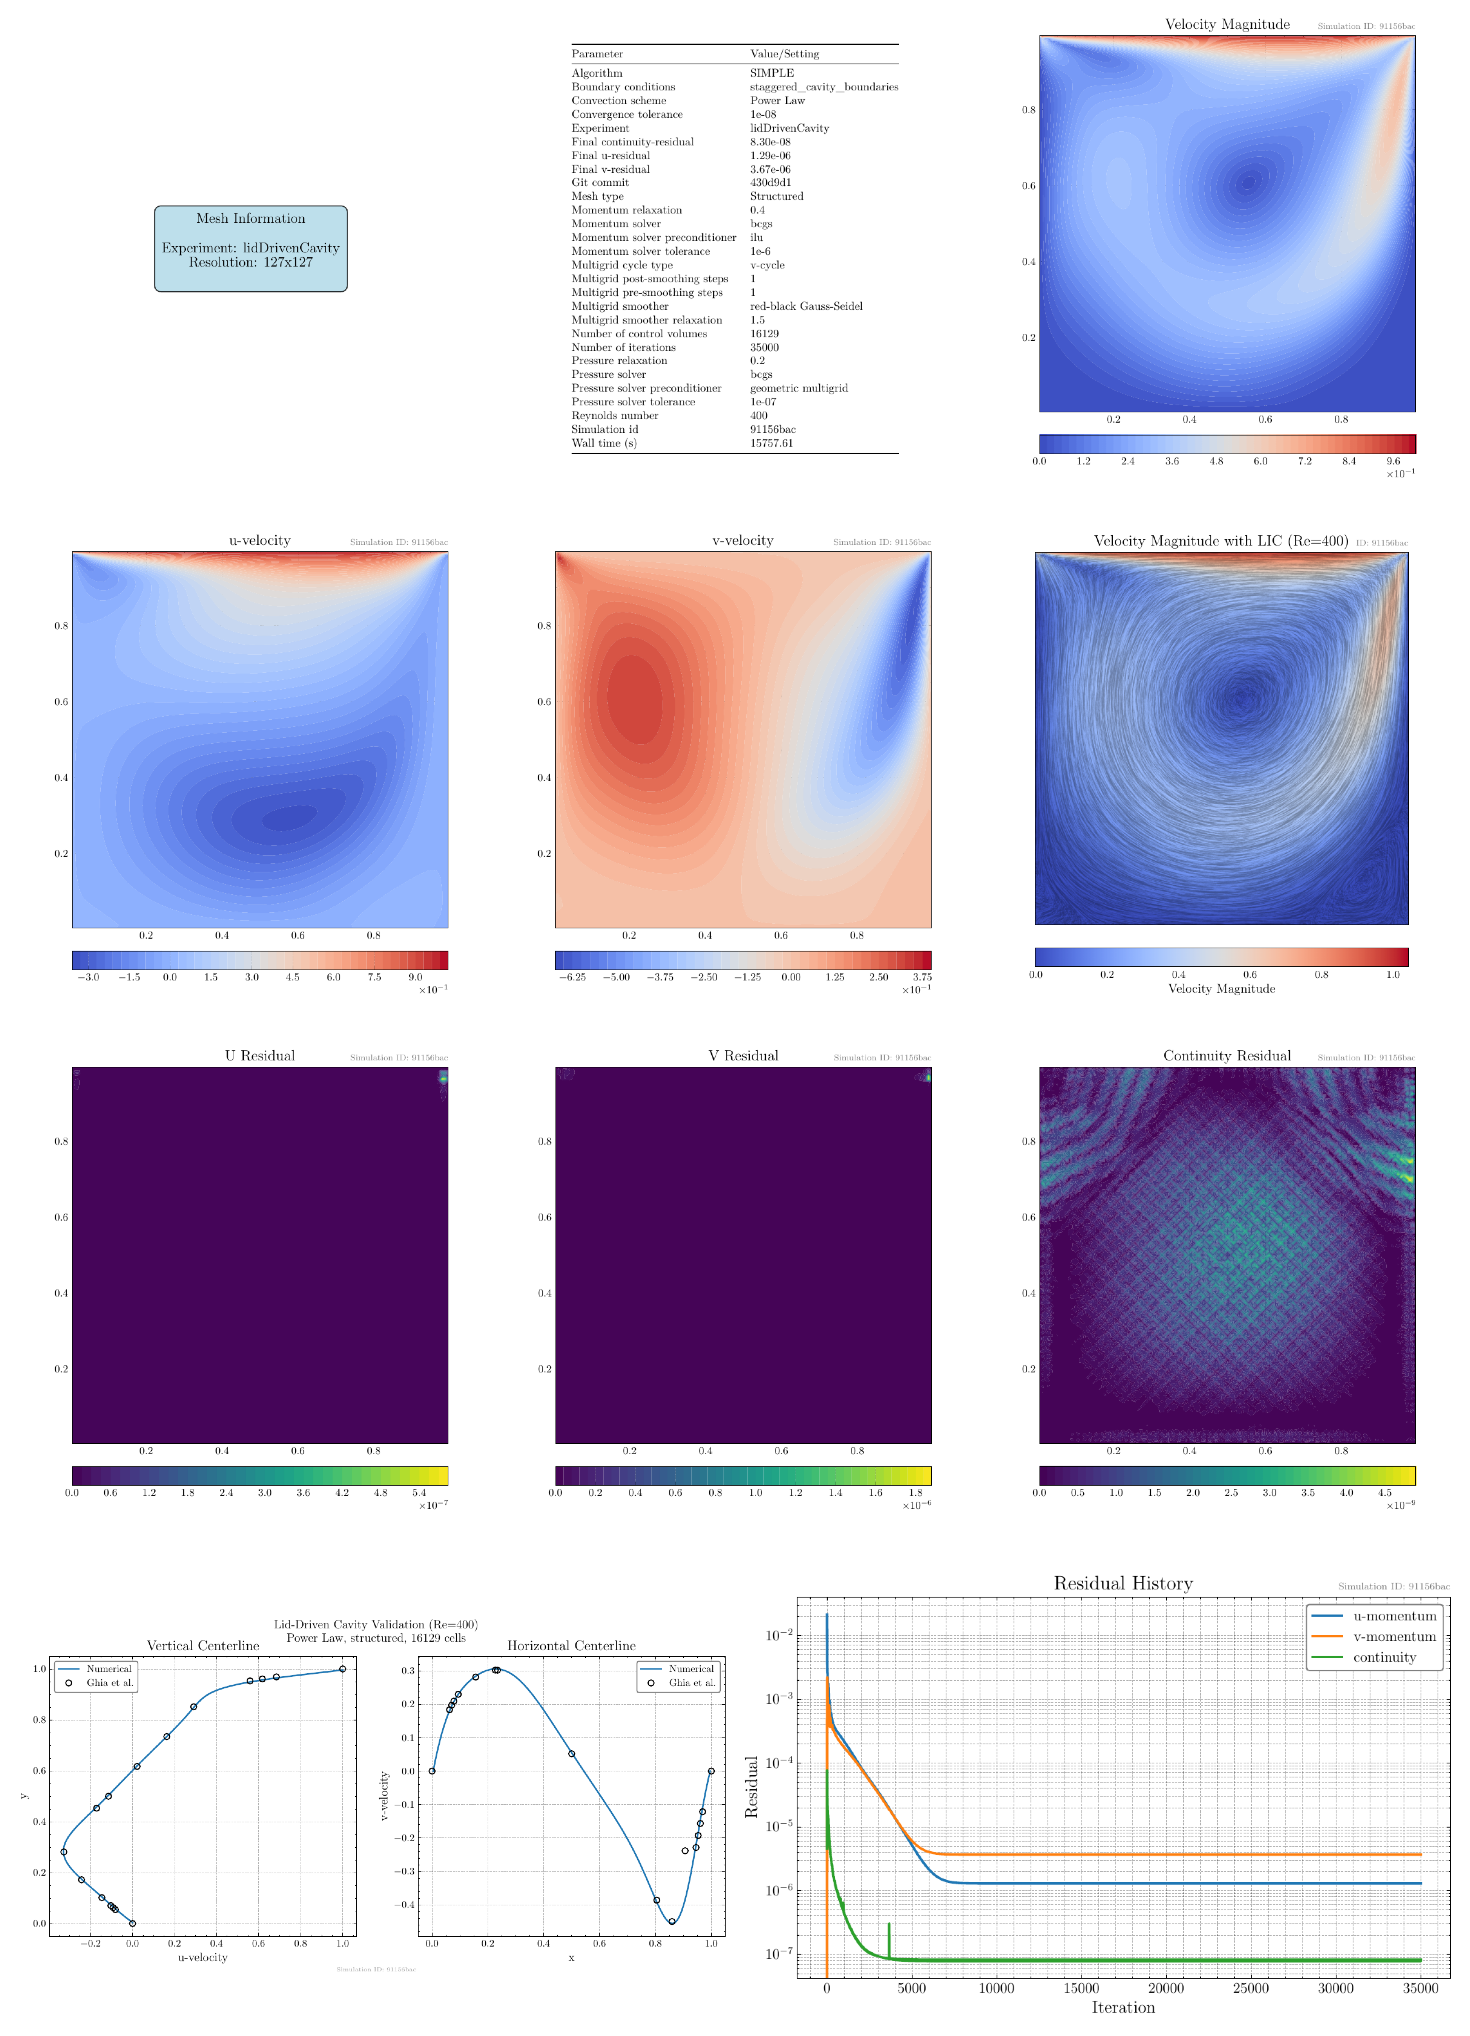
\includegraphics[width=0.85\linewidth]{AppendixPlots/lidDrivenCavity/Re_400/127x127/lidDrivenCavity_Re400_structured_127x127_Power Law_91156bac.pdf}
    \caption{Liddrivencavity simulation at Re=400 using structured 127x127 (medium) mesh with Power Law discretization scheme (Simulation ID: 91156bac)}
    \label{sim.ldc.re400.struct.med.powe}
\end{figure}

\subsection*{Reynolds Number 1000}
\addcontentsline{toc}{subsection}{Reynolds Number 1000}
\label{subsec:liddrivencavity_re1000}

\subsubsection*{Medium Mesh}
\addcontentsline{toc}{subsubsection}{Medium Mesh}
\label{subsubsec:liddrivencavity_re1000_medium}

\paragraph*{Uniform Mesh with QUICK Scheme}
\addcontentsline{toc}{paragraph}{Uniform Mesh with QUICK Scheme}
\label{para:liddrivencavity_re1000_medium_uniform_QUICK}

\begin{figure}[H]
    \centering
    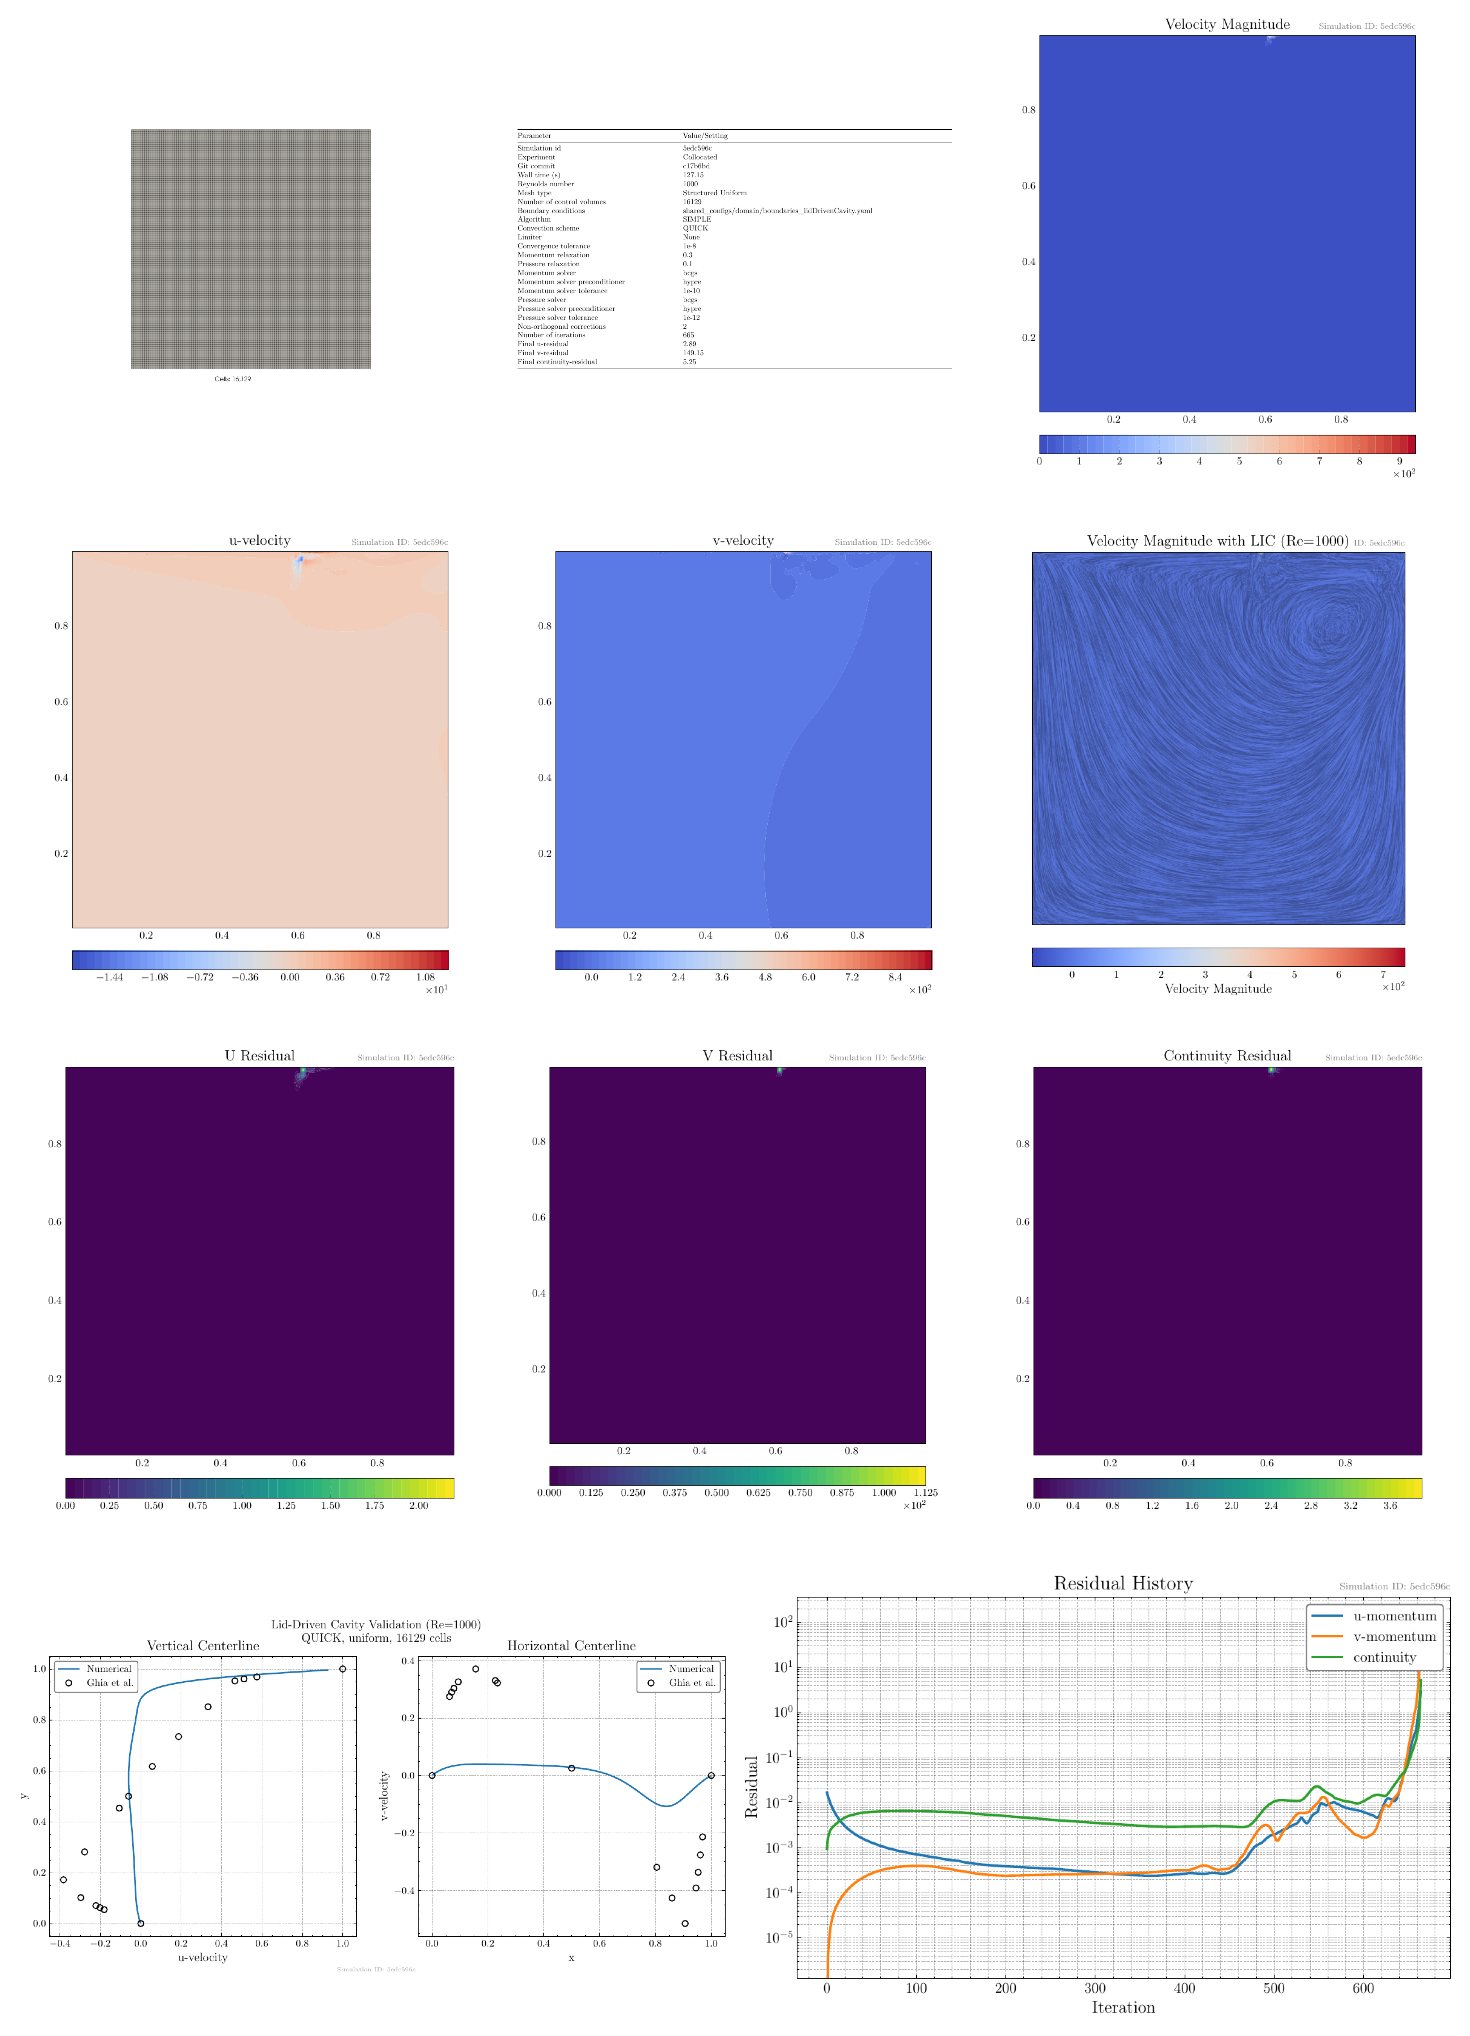
\includegraphics[width=0.85\linewidth]{AppendixPlots/lidDrivenCavity/Re_1000/medium/lidDrivenCavity_Re1000_uniform_medium_QUICK_5edc596c.pdf}
    \caption{Liddrivencavity simulation at Re=1000 using uniform medium mesh with QUICK discretization scheme (Simulation ID: 5edc596c)}
    \label{sim.ldc.re1000.unif.med.quick}
\end{figure}

\paragraph*{Uniform Mesh with TVD Scheme}
\addcontentsline{toc}{paragraph}{Uniform Mesh with TVD Scheme}
\label{para:liddrivencavity_re1000_medium_uniform_TVD}

\begin{figure}[H]
    \centering
    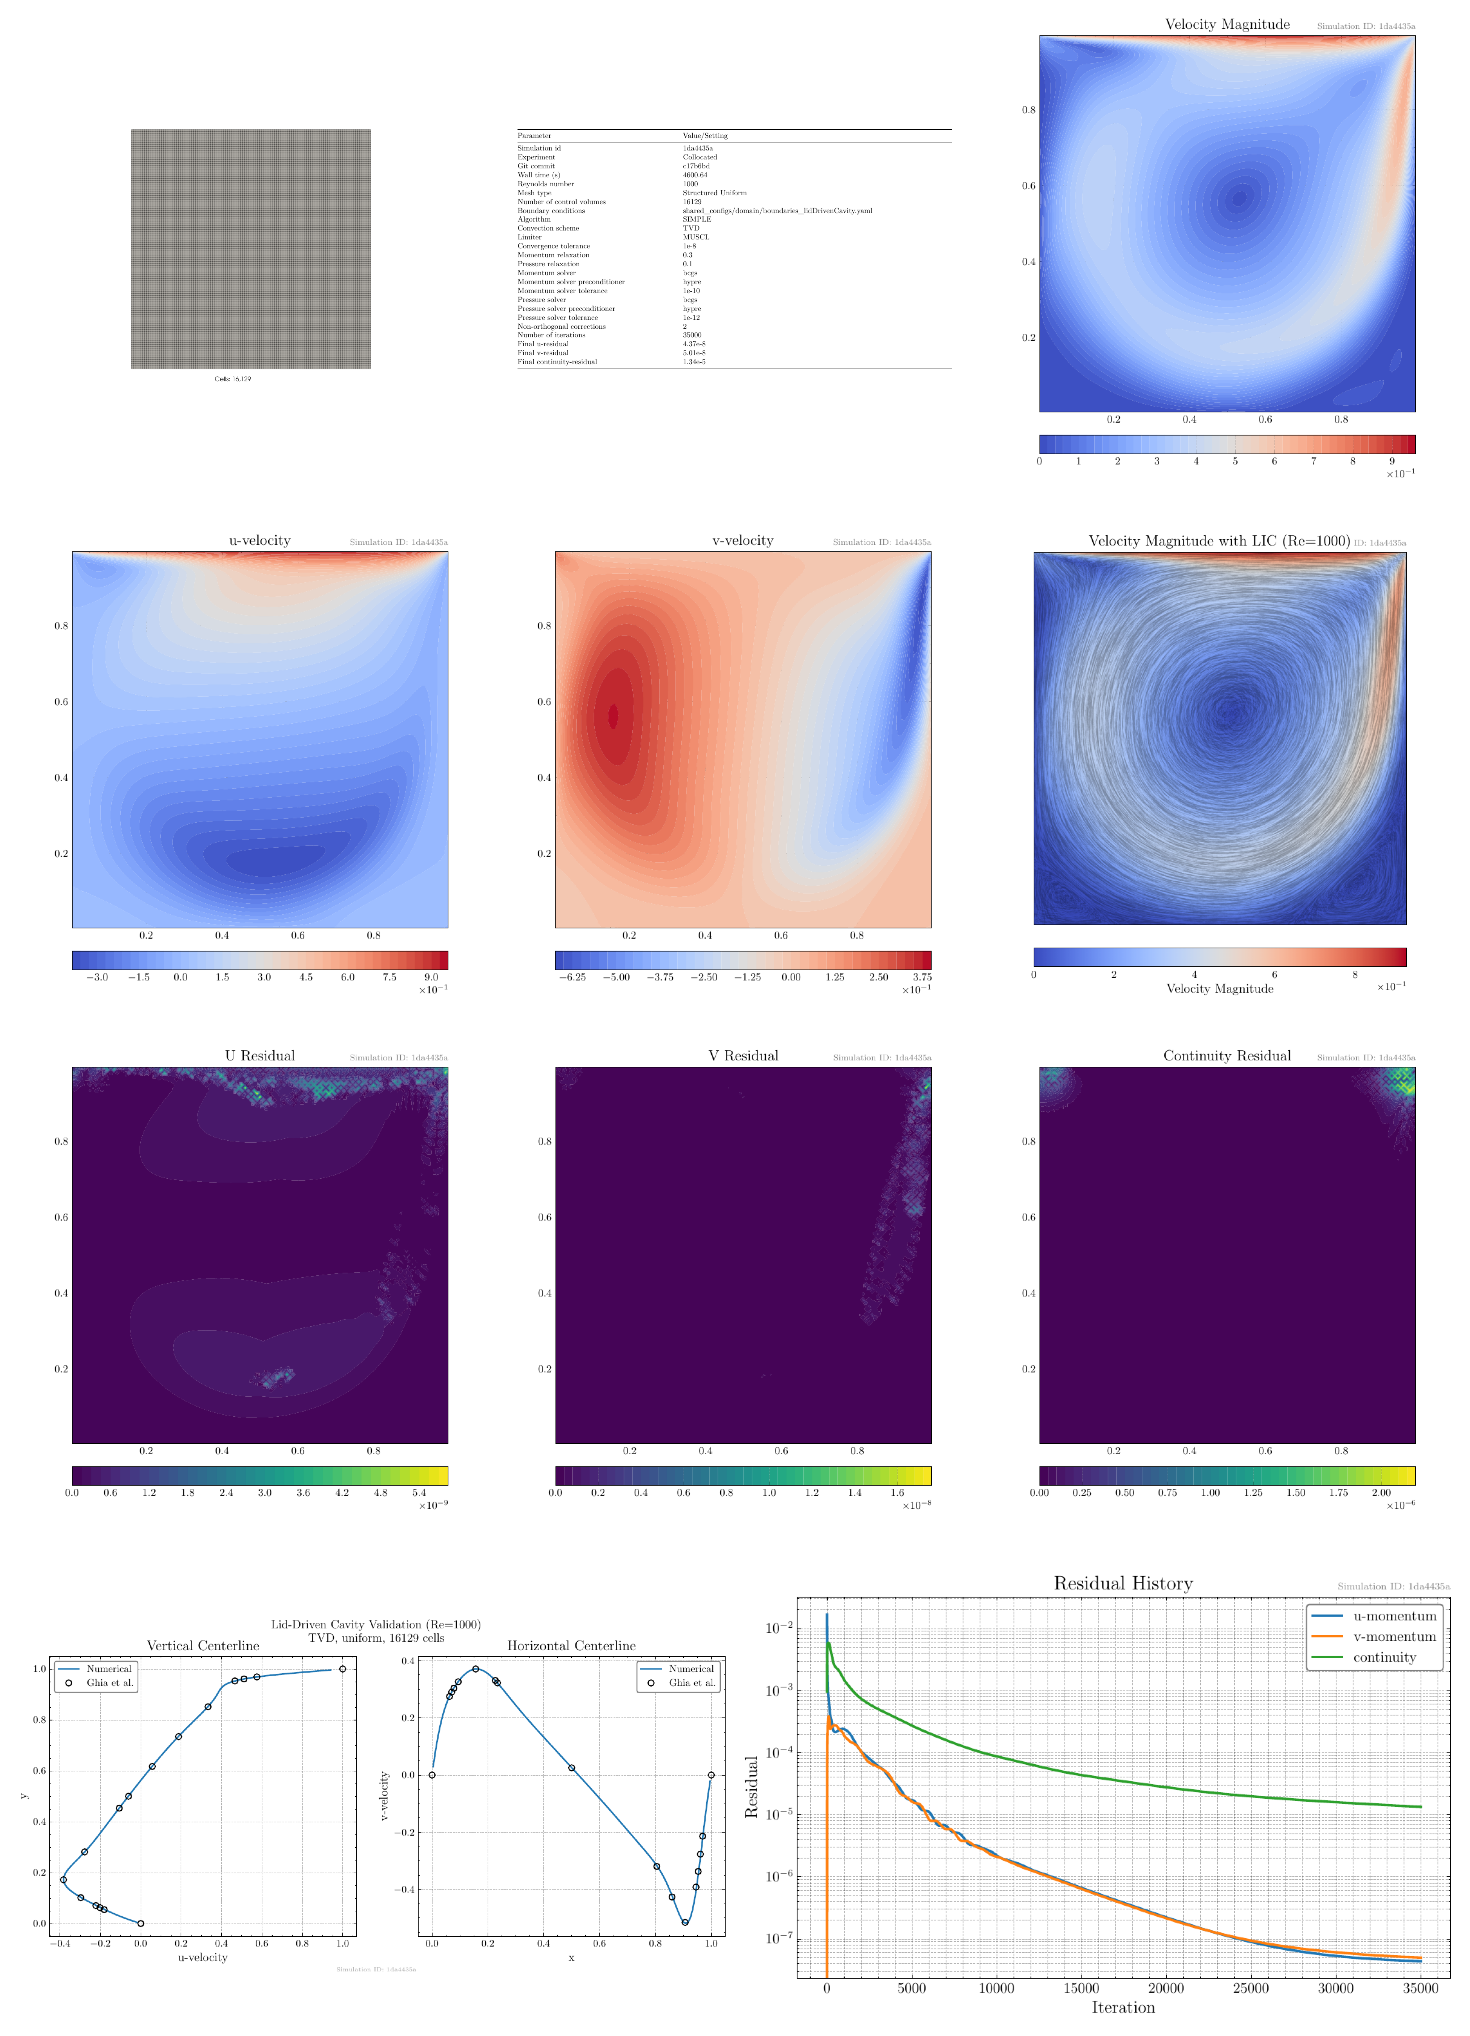
\includegraphics[width=0.85\linewidth]{AppendixPlots/lidDrivenCavity/Re_1000/medium/lidDrivenCavity_Re1000_uniform_medium_TVD_1da4435a.pdf}
    \caption{Liddrivencavity simulation at Re=1000 using uniform medium mesh with TVD discretization scheme (Simulation ID: 1da4435a)}
    \label{sim.ldc.re1000.unif.med.tvd}
\end{figure}

\paragraph*{Uniform Mesh with Upwind Scheme}
\addcontentsline{toc}{paragraph}{Uniform Mesh with Upwind Scheme}
\label{para:liddrivencavity_re1000_medium_uniform_Upwind}

\begin{figure}[H]
    \centering
    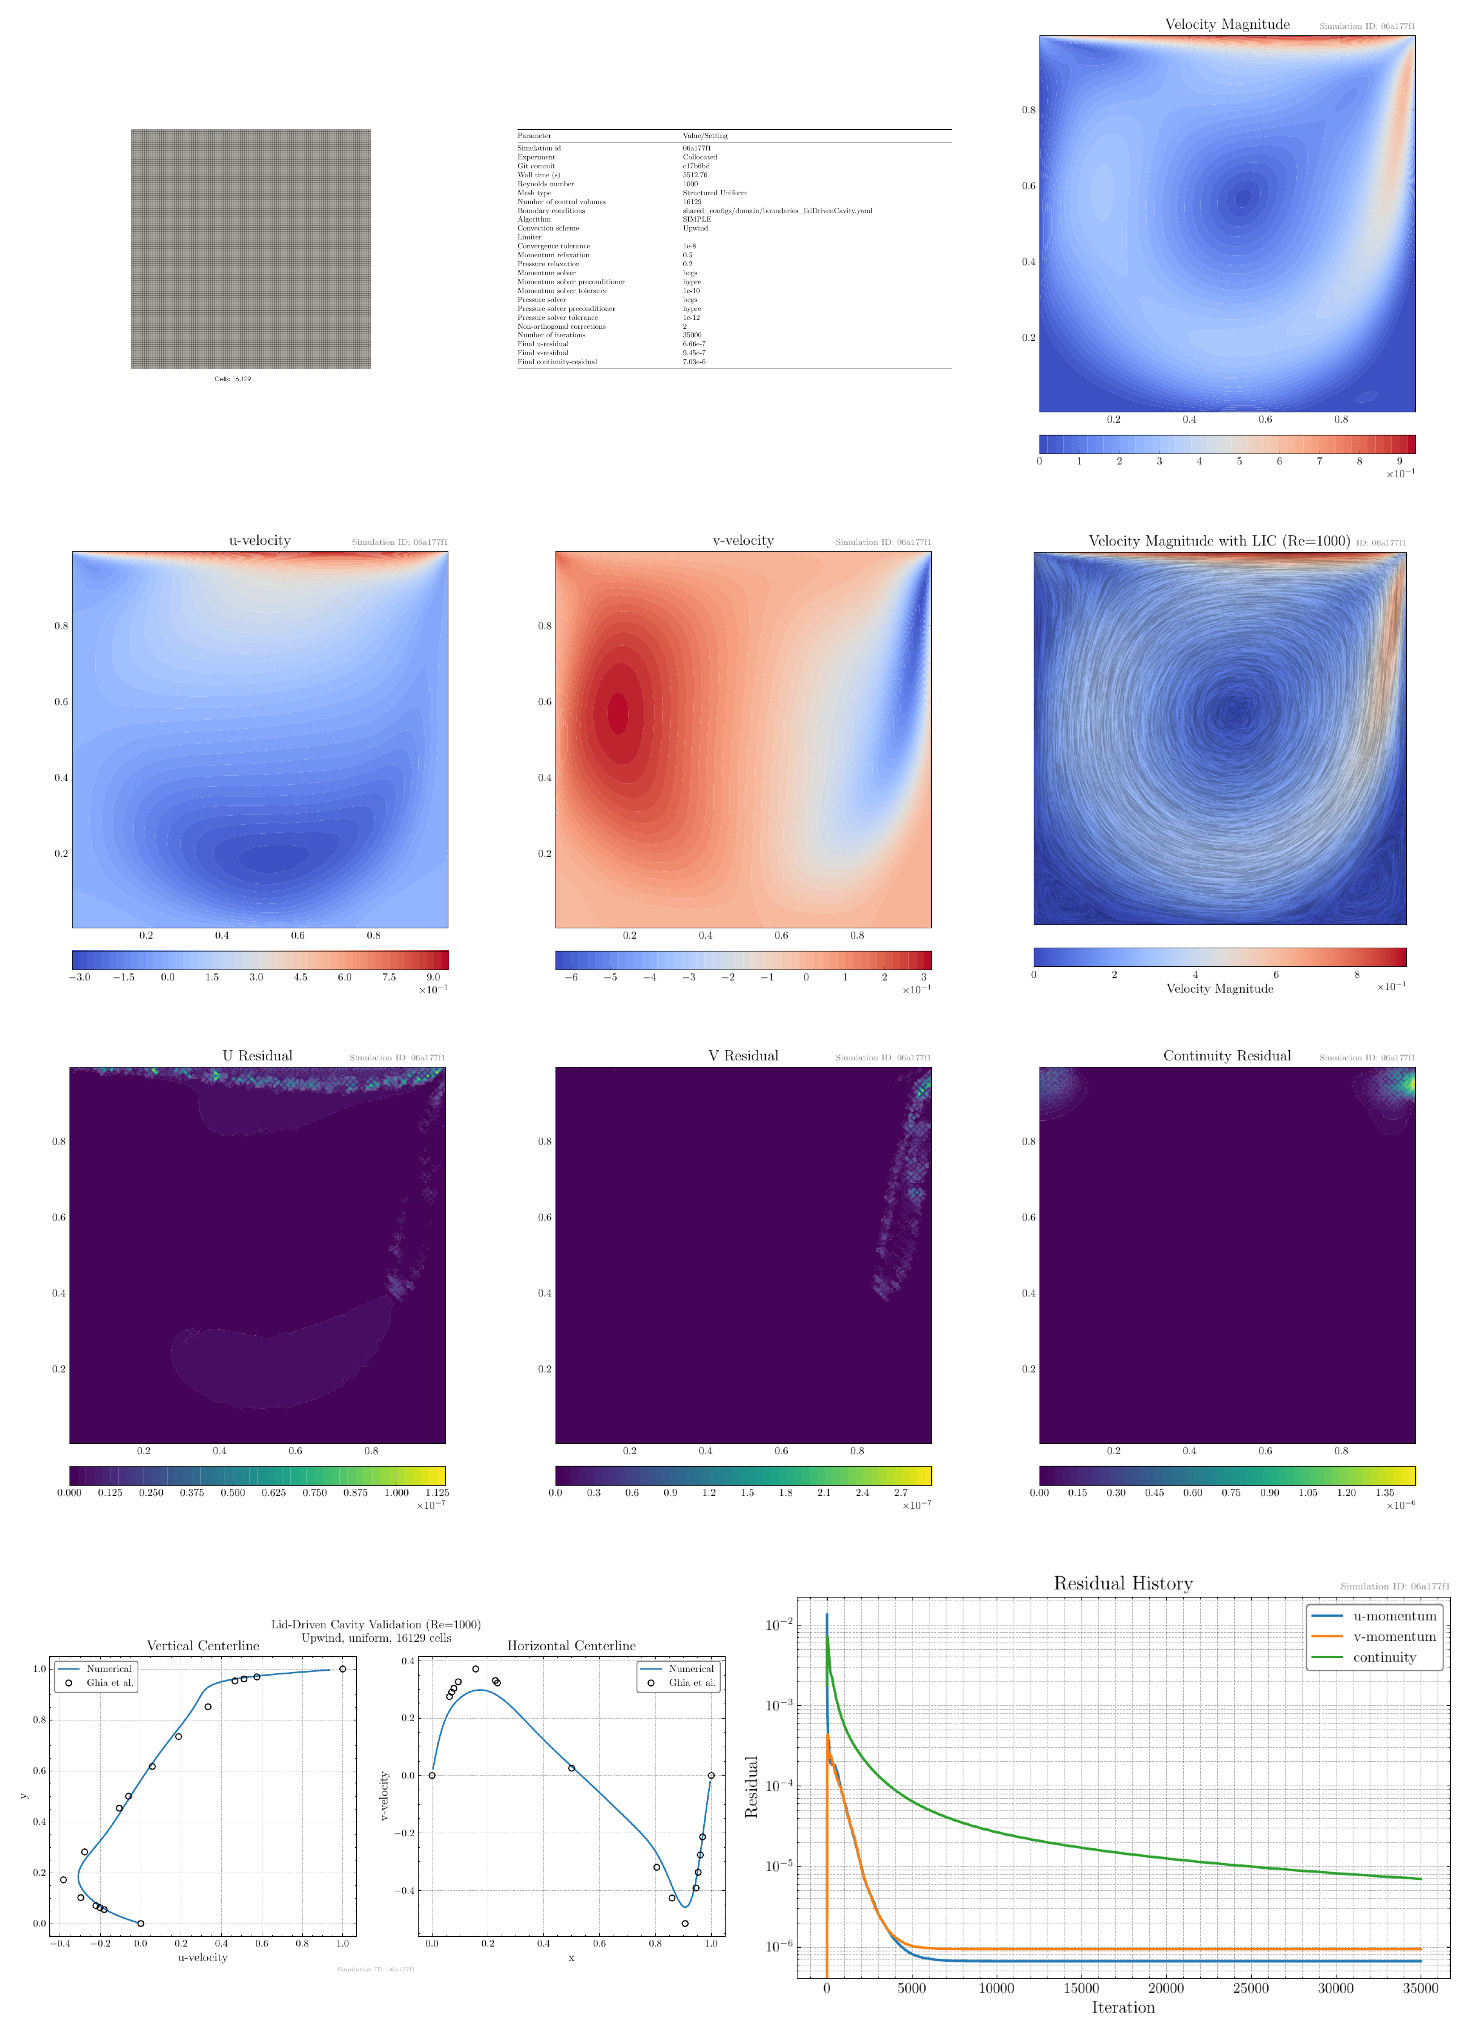
\includegraphics[width=0.85\linewidth]{AppendixPlots/lidDrivenCavity/Re_1000/medium/lidDrivenCavity_Re1000_uniform_medium_Upwind_06a177f1.pdf}
    \caption{Liddrivencavity simulation at Re=1000 using uniform medium mesh with Upwind discretization scheme (Simulation ID: 06a177f1)}
    \label{sim.ldc.re1000.unif.med.upwind}
\end{figure}

\paragraph*{Unstructured Mesh with QUICK Scheme}
\addcontentsline{toc}{paragraph}{Unstructured Mesh with QUICK Scheme}
\label{para:liddrivencavity_re1000_medium_unstructured_QUICK}

\begin{figure}[H]
    \centering
    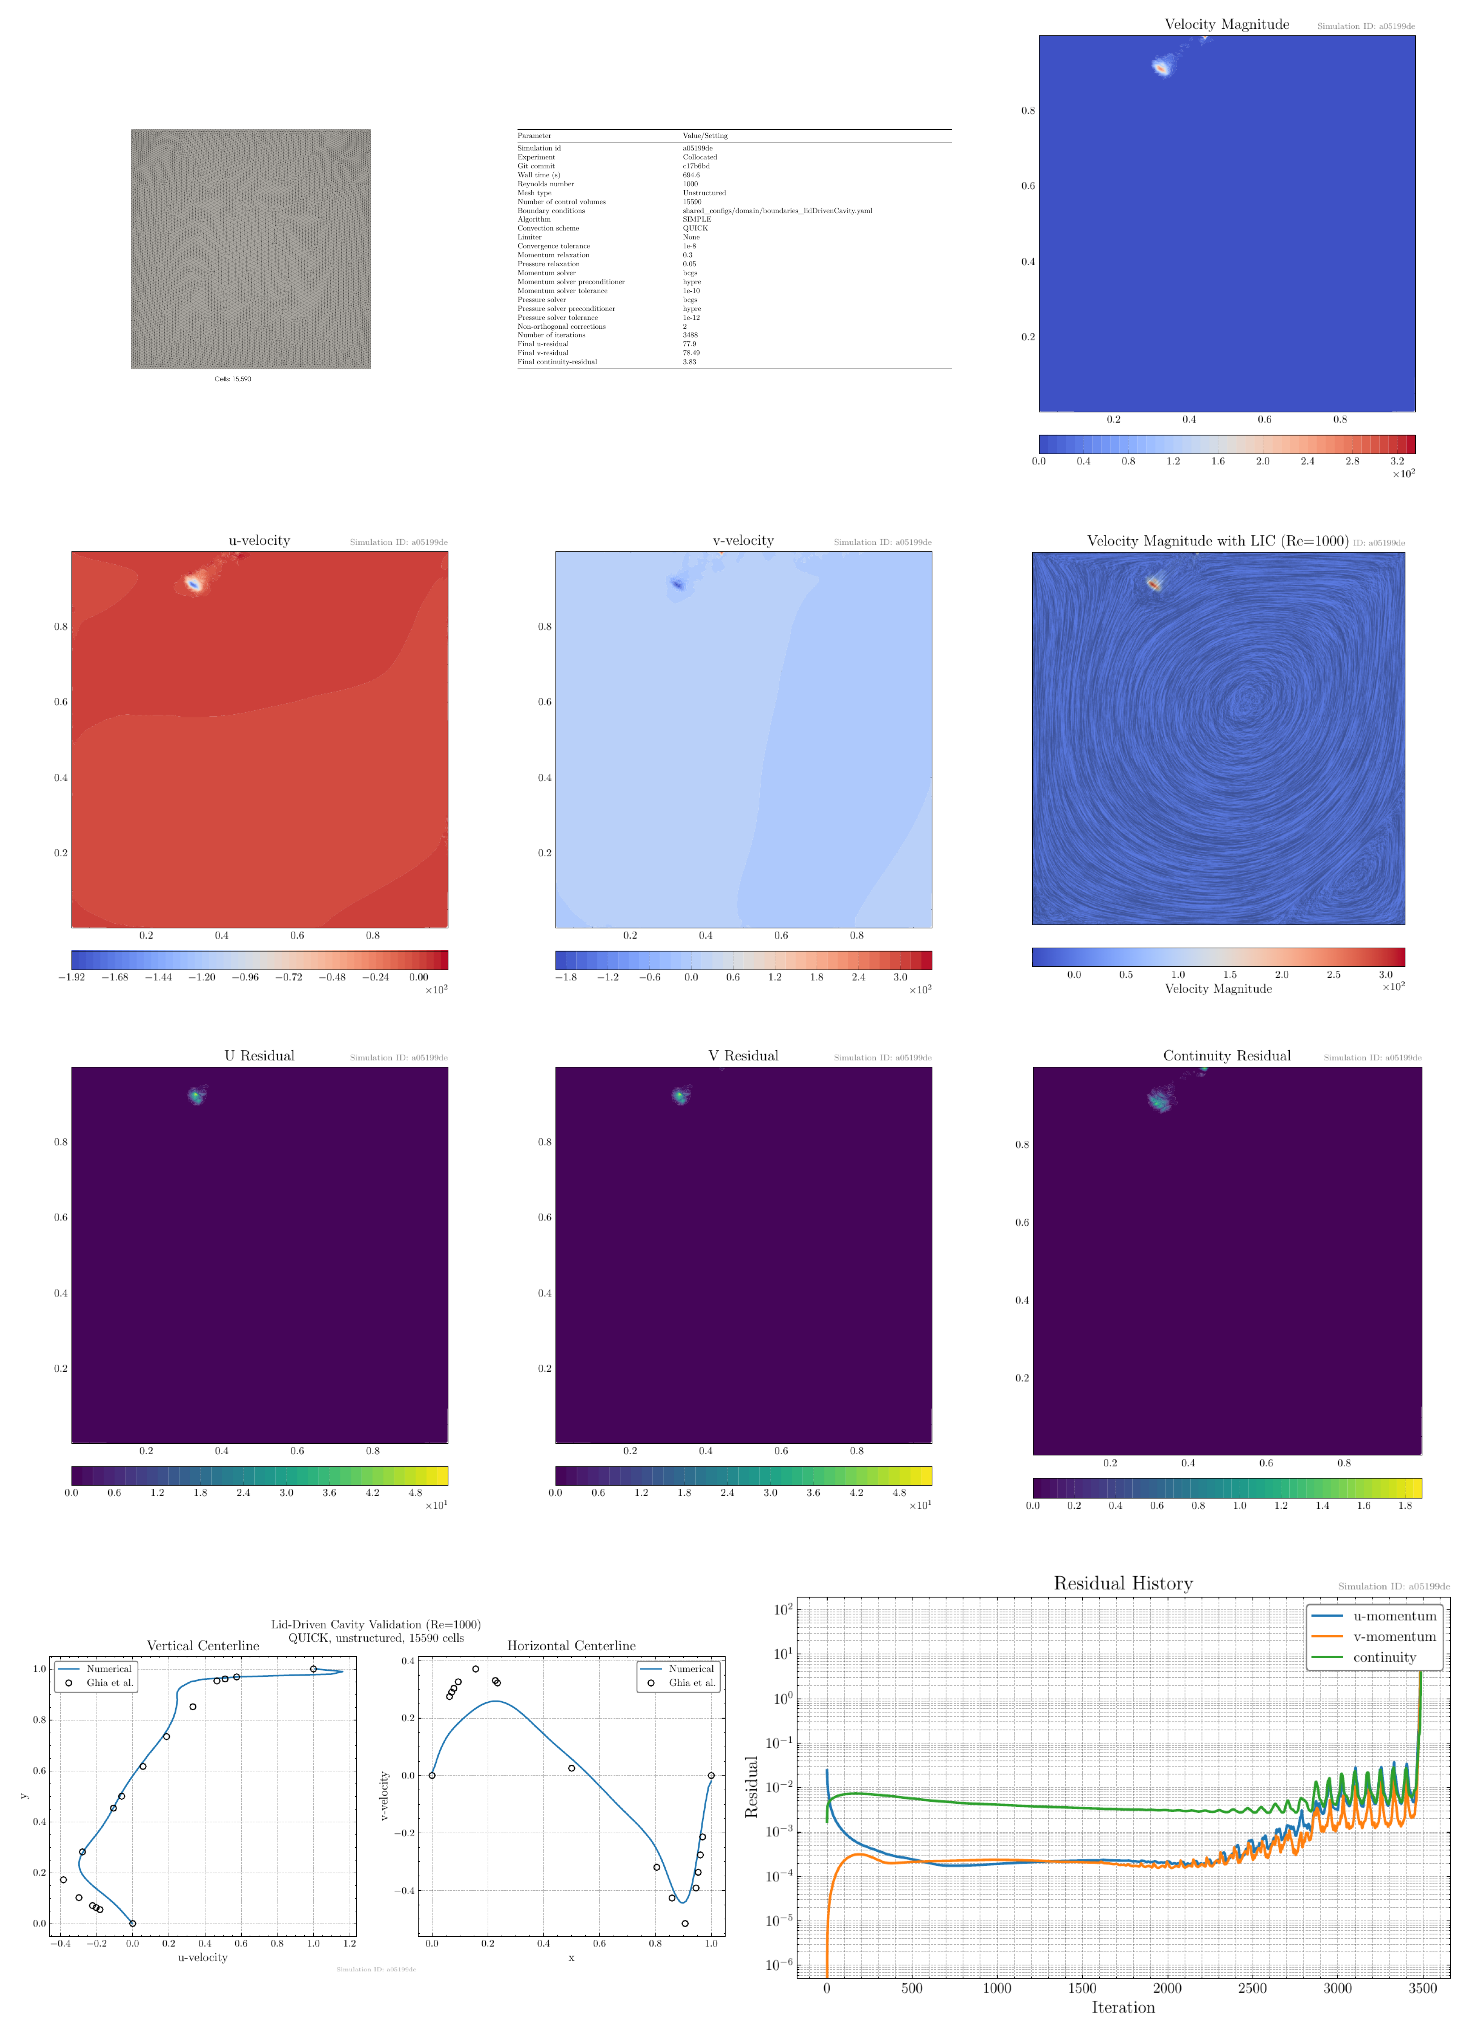
\includegraphics[width=0.85\linewidth]{AppendixPlots/lidDrivenCavity/Re_1000/medium/lidDrivenCavity_Re1000_unstructured_medium_QUICK_a05199de.pdf}
    \caption{Liddrivencavity simulation at Re=1000 using unstructured medium mesh with QUICK discretization scheme (Simulation ID: a05199de)}
    \label{sim.ldc.re1000.unstruct.med.quick}
\end{figure}

\paragraph*{Unstructured Mesh with Upwind Scheme}
\addcontentsline{toc}{paragraph}{Unstructured Mesh with Upwind Scheme}
\label{para:liddrivencavity_re1000_medium_unstructured_Upwind}

\begin{figure}[H]
    \centering
    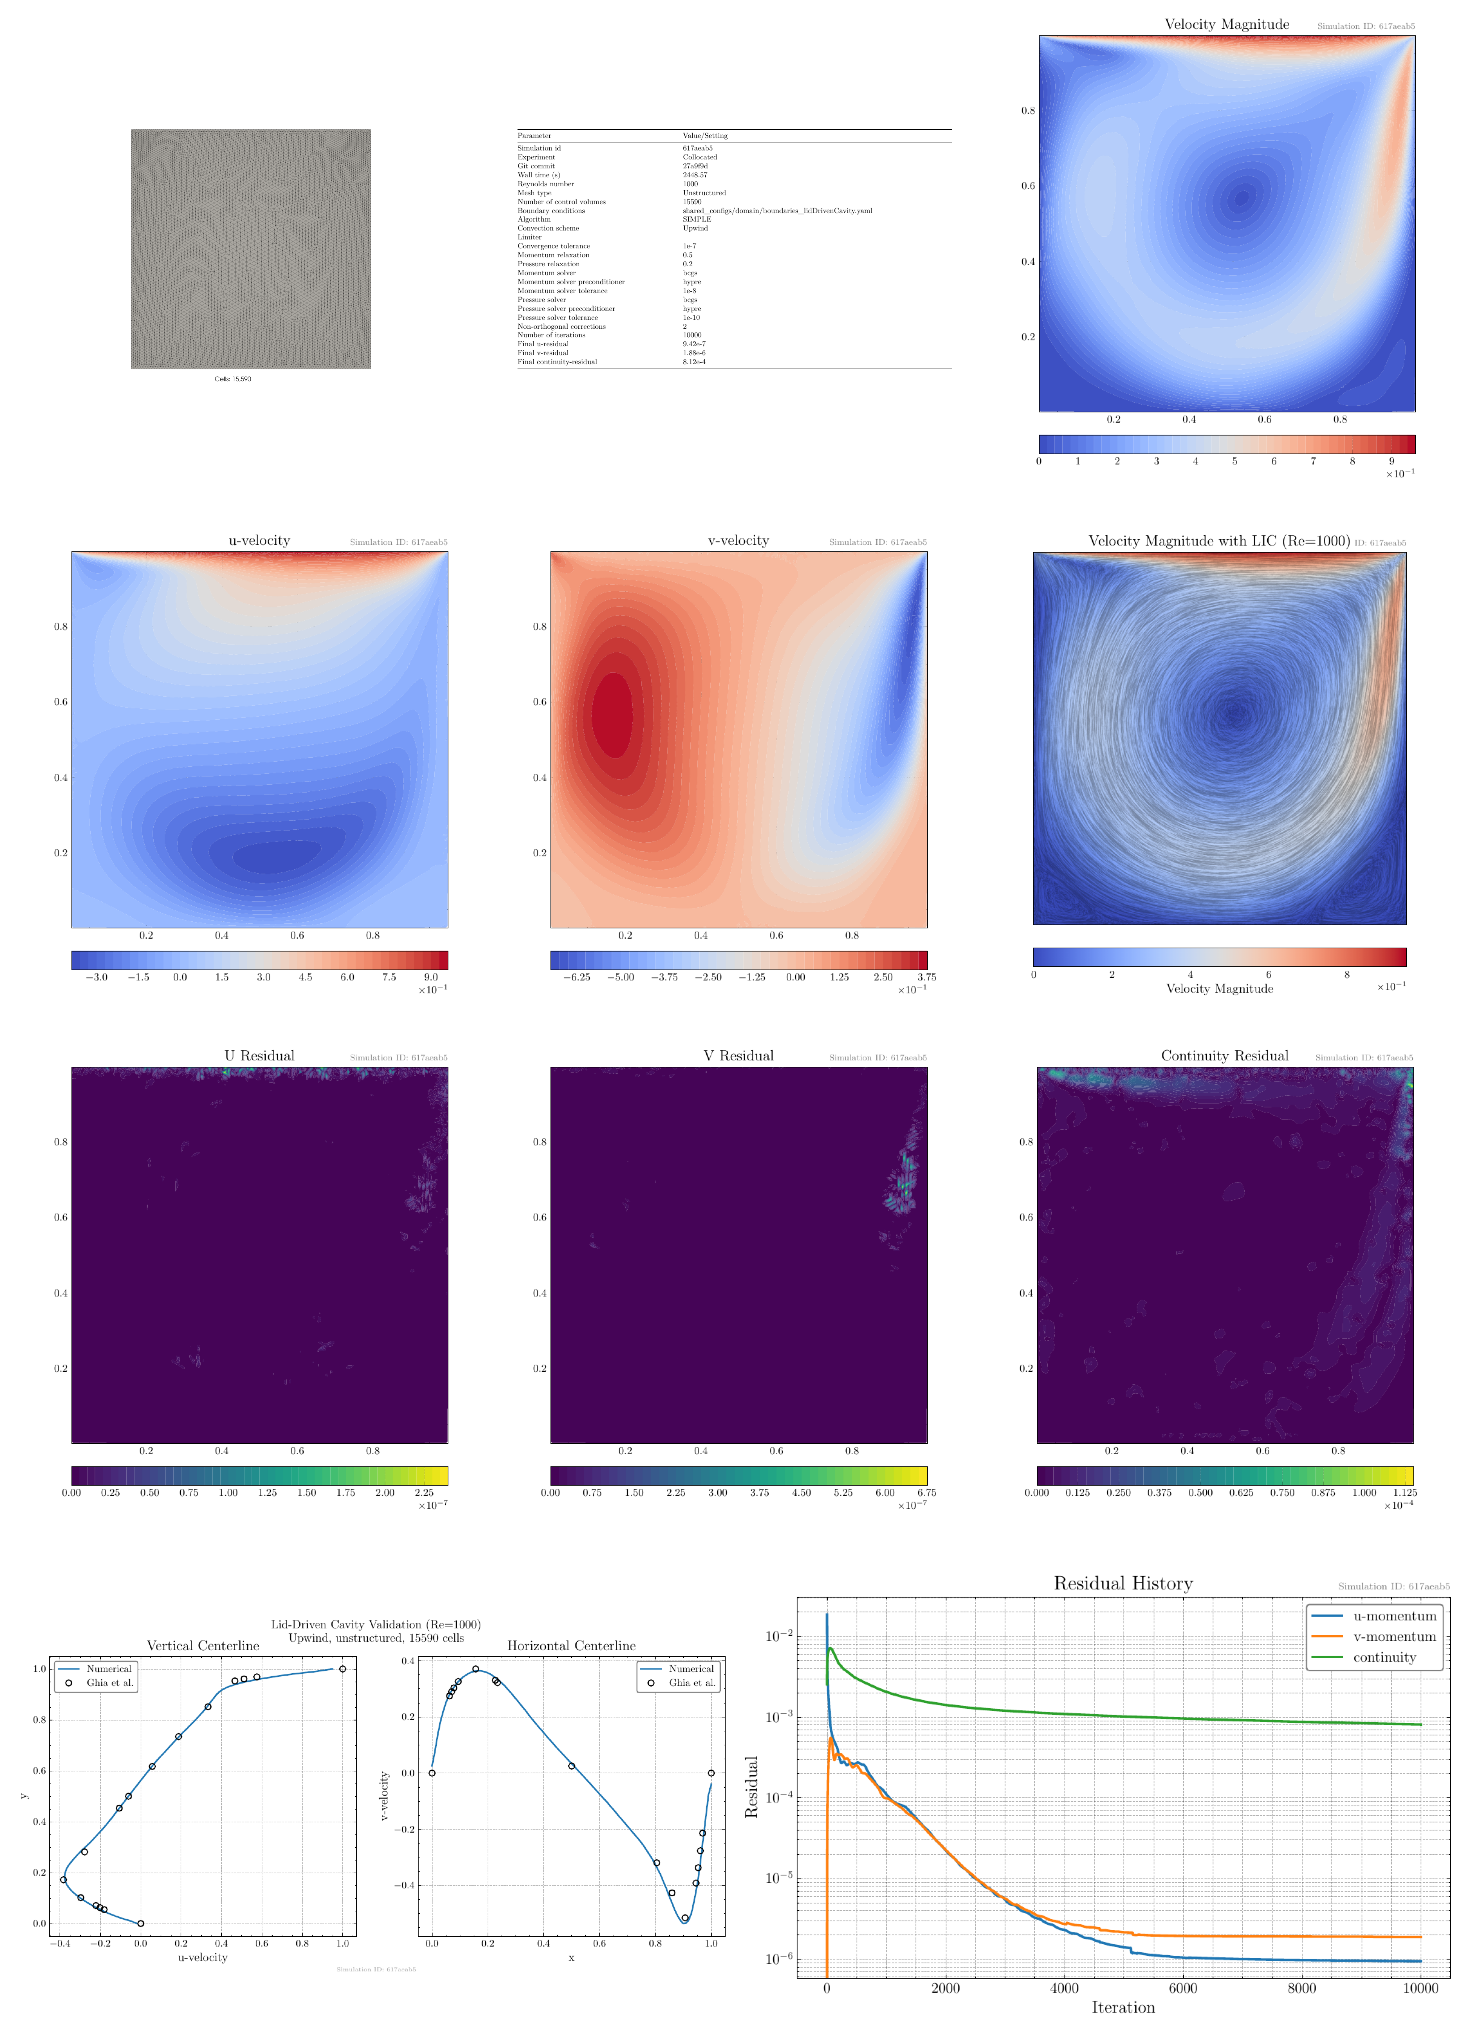
\includegraphics[width=0.85\linewidth]{AppendixPlots/lidDrivenCavity/Re_1000/medium/lidDrivenCavity_Re1000_unstructured_medium_Upwind_617aeab5.pdf}
    \caption{Liddrivencavity simulation at Re=1000 using unstructured medium mesh with Upwind discretization scheme (Simulation ID: 617aeab5)}
    \label{sim.ldc.re1000.unstruct.med.upwind}
\end{figure}

\clearpage

\subsubsection*{Fine Mesh}
\addcontentsline{toc}{subsubsection}{Fine Mesh}
\label{subsubsec:liddrivencavity_re1000_fine}

\paragraph*{Uniform Mesh with TVD Scheme}
\addcontentsline{toc}{paragraph}{Uniform Mesh with TVD Scheme}
\label{para:liddrivencavity_re1000_fine_uniform_TVD}

\begin{figure}[H]
    \centering
    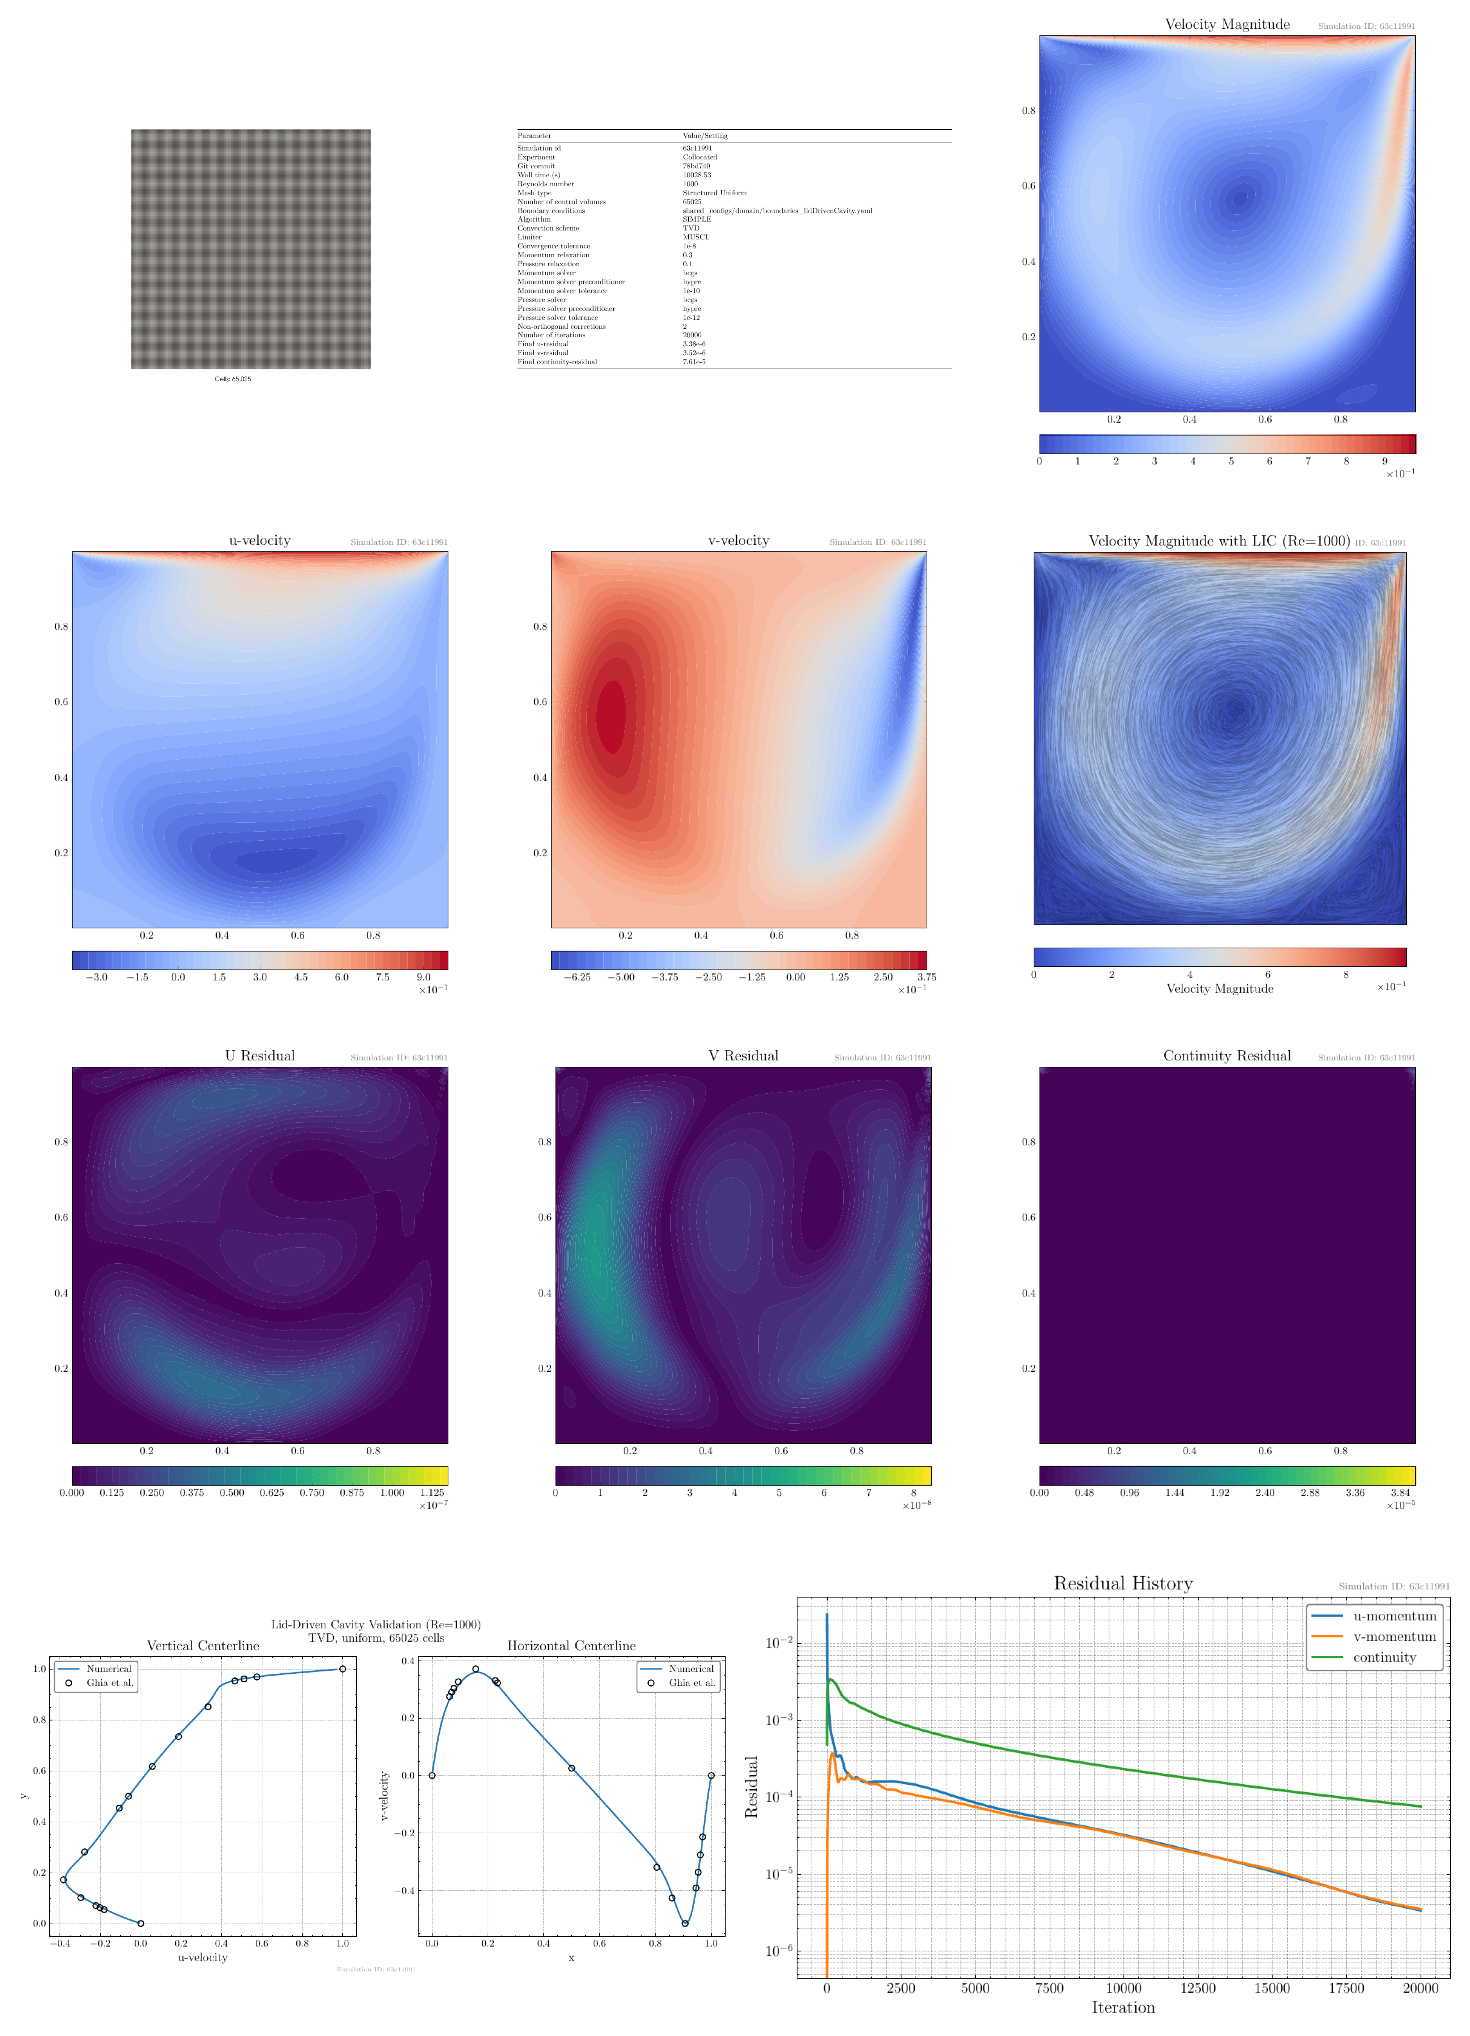
\includegraphics[width=0.85\linewidth]{AppendixPlots/lidDrivenCavity/Re_1000/fine/lidDrivenCavity_Re1000_uniform_fine_TVD_63c11991.pdf}
    \caption{Liddrivencavity simulation at Re=1000 using uniform fine mesh with TVD discretization scheme (Simulation ID: 63c11991)}
    \label{sim.ldc.re1000.unif.fine.tvd}
\end{figure}

\paragraph*{Uniform Mesh with Upwind Scheme}
\addcontentsline{toc}{paragraph}{Uniform Mesh with Upwind Scheme}
\label{para:liddrivencavity_re1000_fine_uniform_Upwind}

\begin{figure}[H]
    \centering
    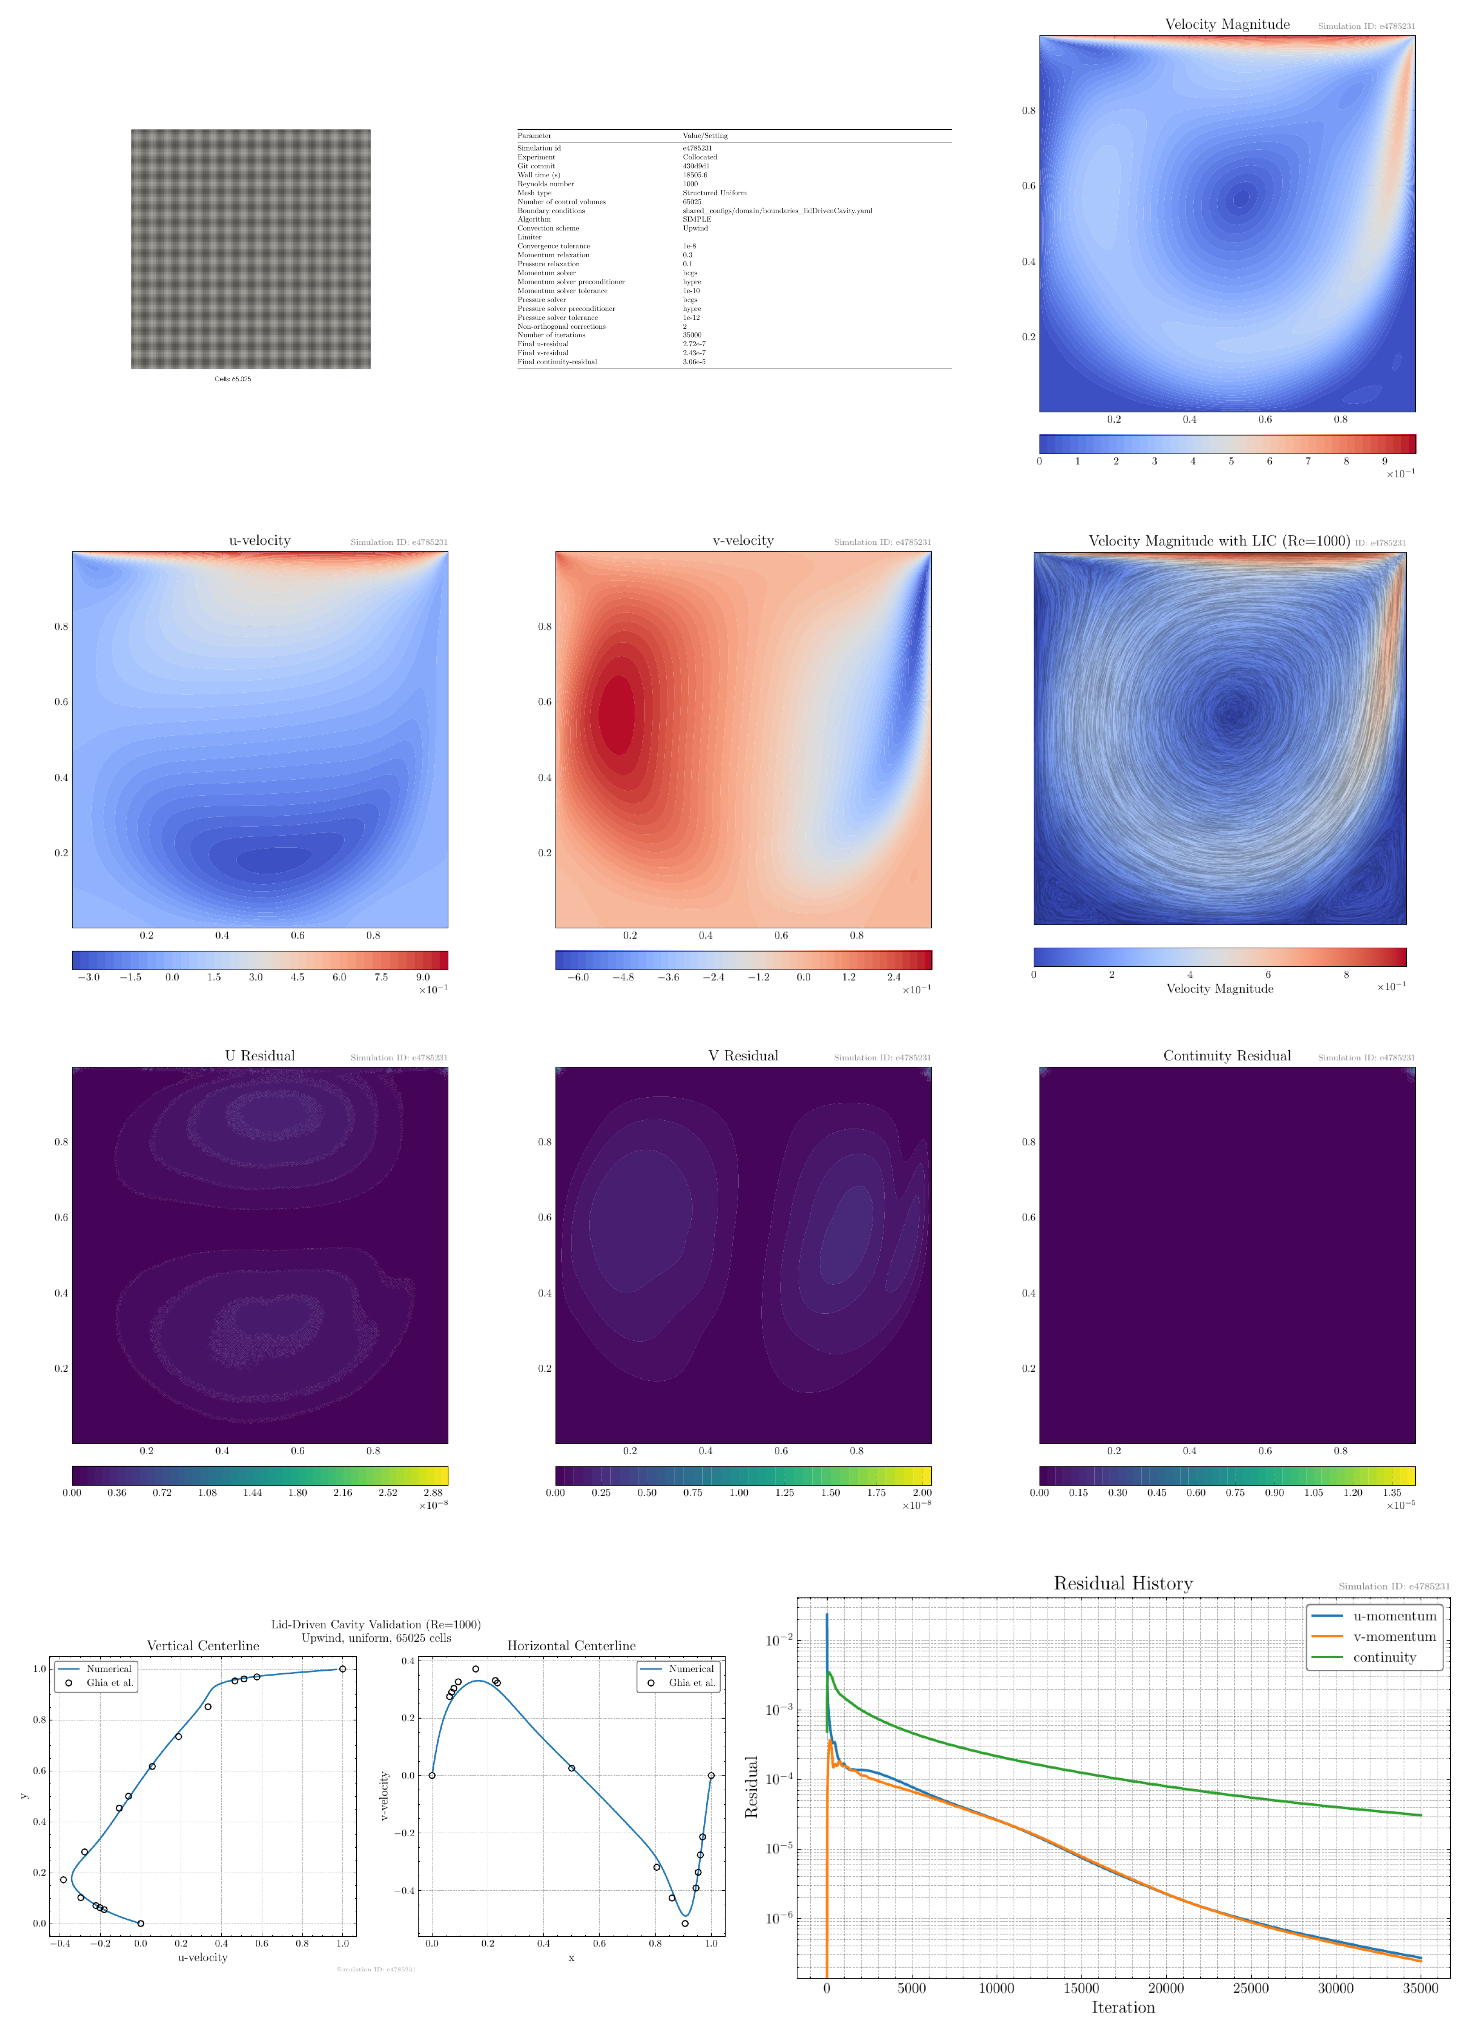
\includegraphics[width=0.85\linewidth]{AppendixPlots/lidDrivenCavity/Re_1000/fine/lidDrivenCavity_Re1000_uniform_fine_Upwind_e4785231.pdf}
    \caption{Liddrivencavity simulation at Re=1000 using uniform fine mesh with Upwind discretization scheme (Simulation ID: e4785231)}
    \label{sim.ldc.re1000.unif.fine.upwind}
\end{figure}

\paragraph*{Unstructured Mesh with TVD Scheme}
\addcontentsline{toc}{paragraph}{Unstructured Mesh with TVD Scheme}
\label{para:liddrivencavity_re1000_fine_unstructured_TVD}

\begin{figure}[H]
    \centering
    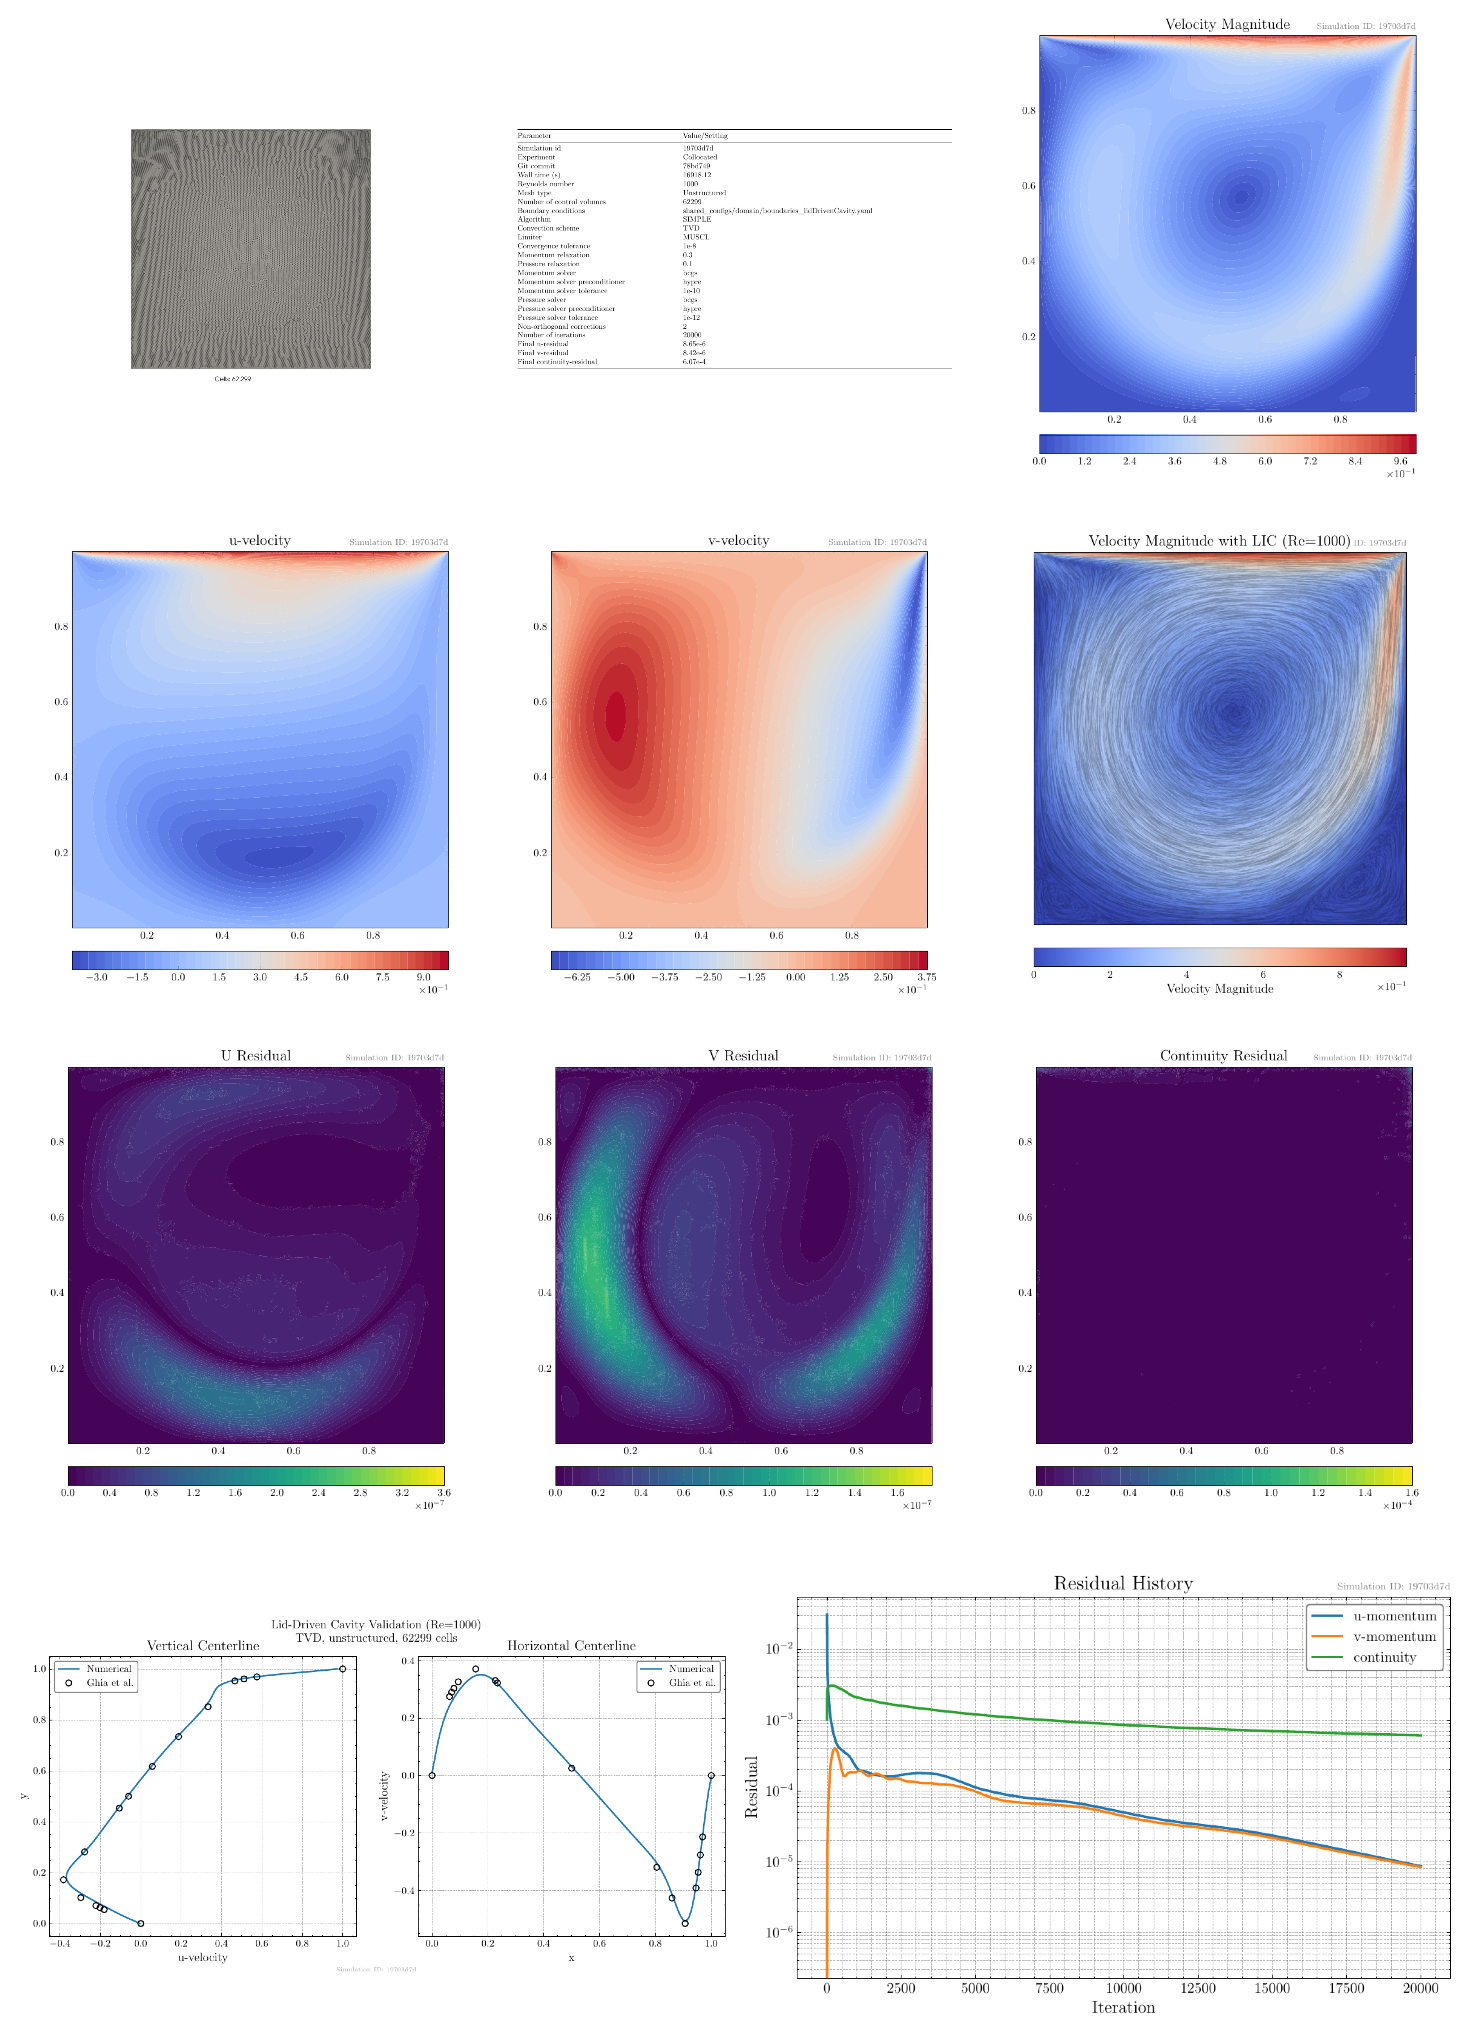
\includegraphics[width=0.85\linewidth]{AppendixPlots/lidDrivenCavity/Re_1000/fine/lidDrivenCavity_Re1000_unstructured_fine_TVD_19703d7d.pdf}
    \caption{Liddrivencavity simulation at Re=1000 using unstructured fine mesh with TVD discretization scheme (Simulation ID: 19703d7d)}
    \label{sim.ldc.re1000.unstruct.fine.tvd}
\end{figure}

\paragraph*{Unstructured Mesh with Upwind Scheme}
\addcontentsline{toc}{paragraph}{Unstructured Mesh with Upwind Scheme}
\label{para:liddrivencavity_re1000_fine_unstructured_Upwind}

\begin{figure}[H]
    \centering
    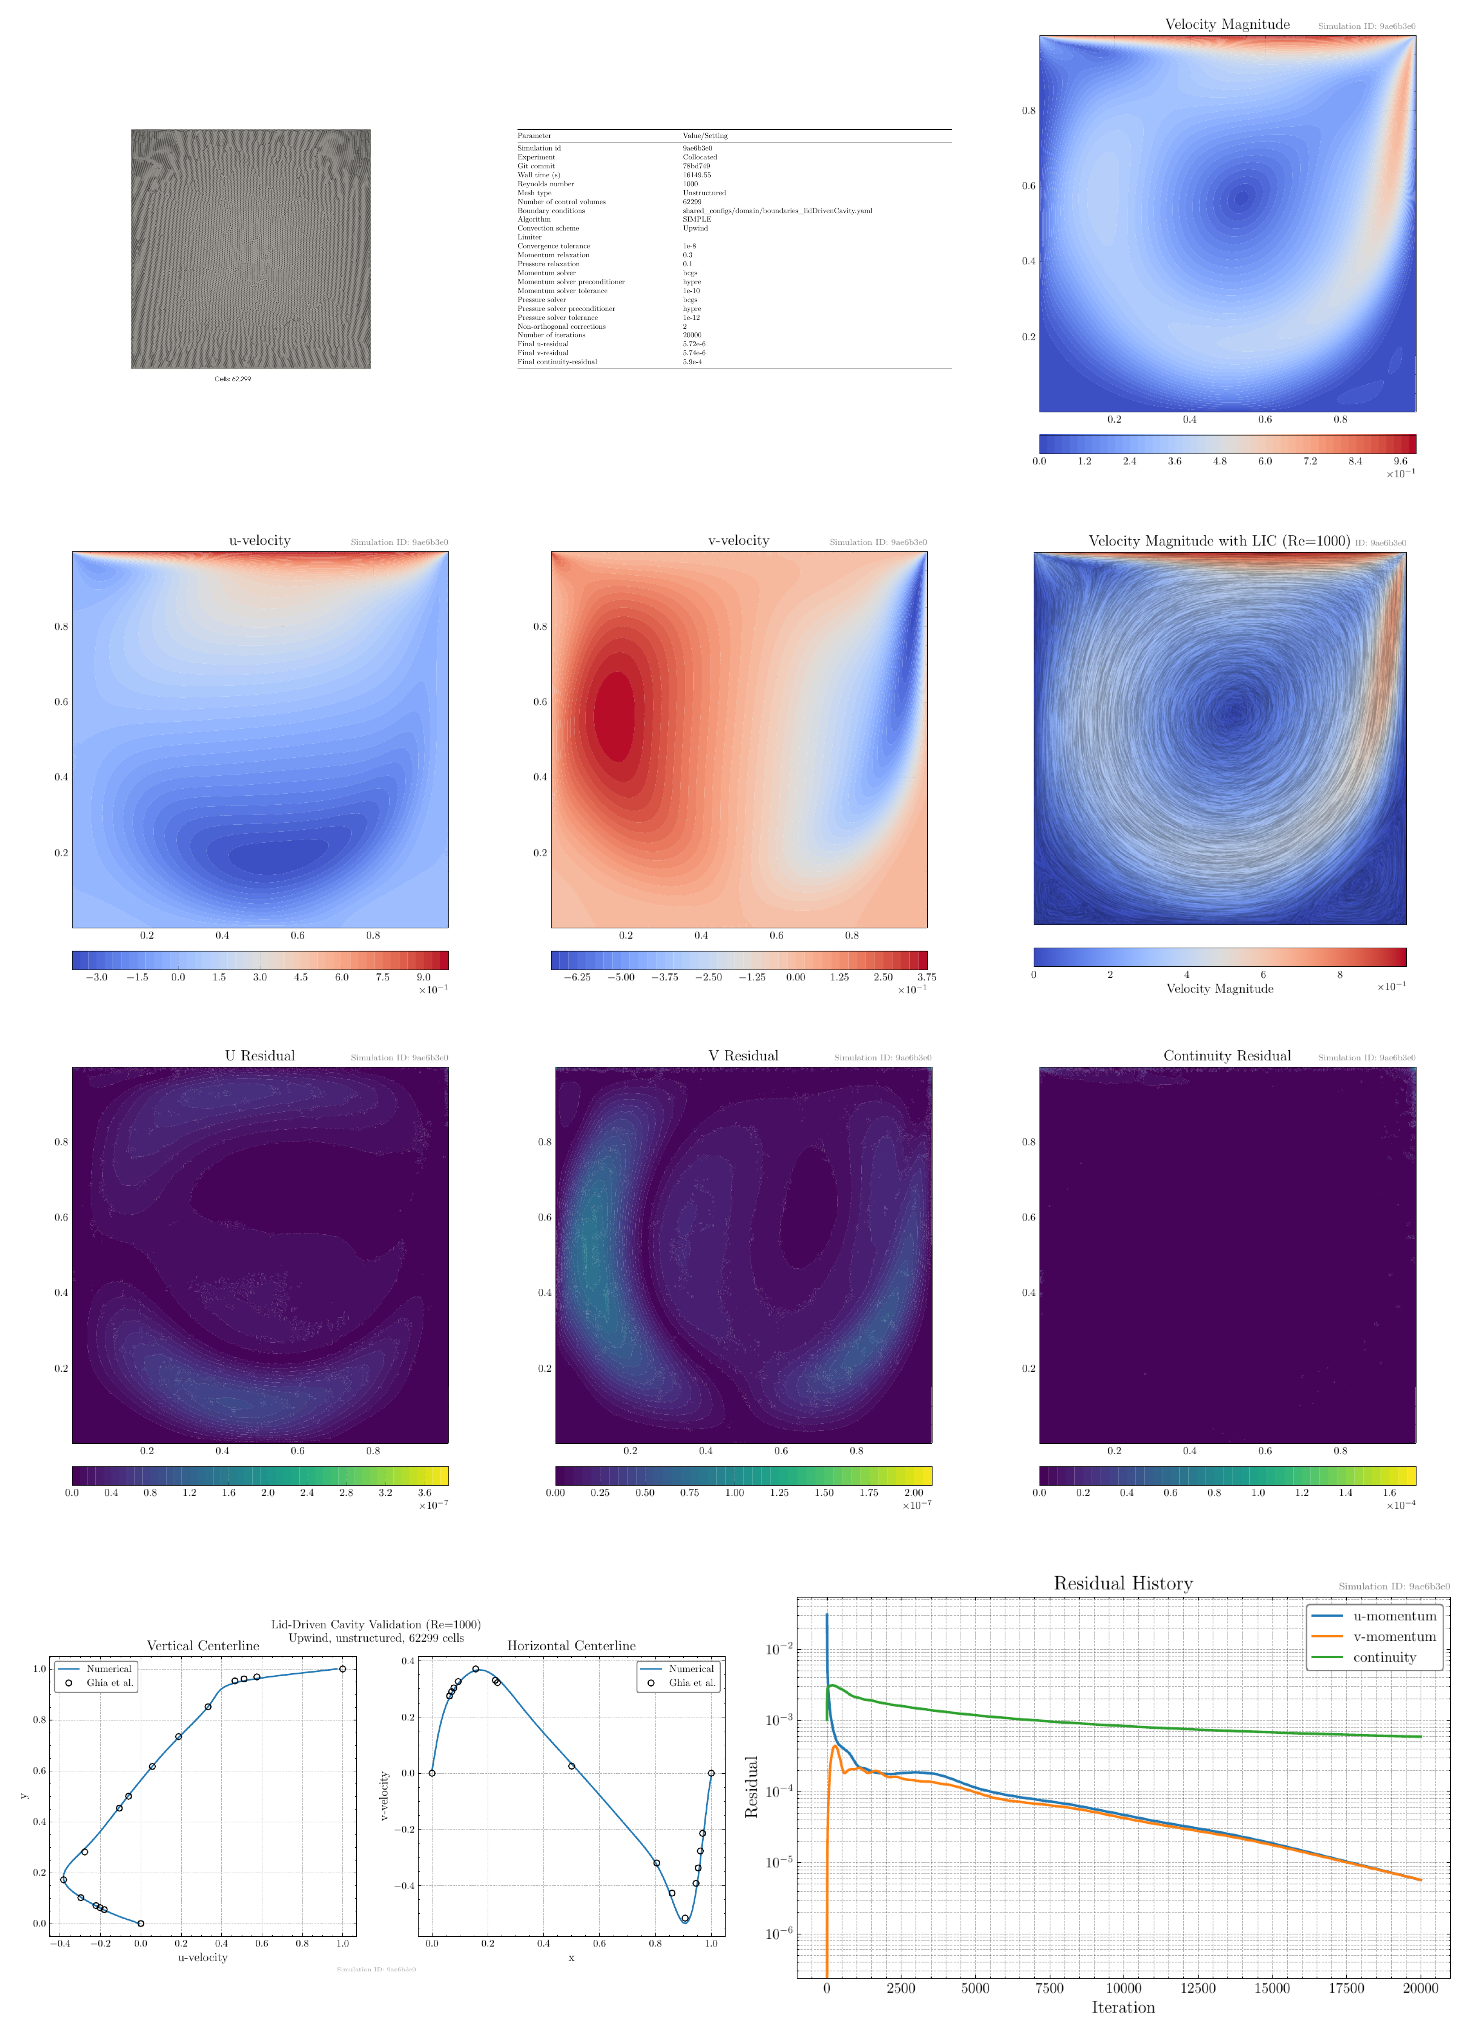
\includegraphics[width=0.85\linewidth]{AppendixPlots/lidDrivenCavity/Re_1000/fine/lidDrivenCavity_Re1000_unstructured_fine_Upwind_9ae6b3e0.pdf}
    \caption{Liddrivencavity simulation at Re=1000 using unstructured fine mesh with Upwind discretization scheme (Simulation ID: 9ae6b3e0)}
    \label{sim.ldc.re1000.unstruct.fine.upwind}
\end{figure}

\clearpage

\subsubsection*{127X127 Mesh}
\addcontentsline{toc}{subsubsection}{127X127 Mesh}
\label{subsubsec:liddrivencavity_re1000_127x127}

\paragraph*{Structured Mesh with Power Law Scheme}
\addcontentsline{toc}{paragraph}{Structured Mesh with Power Law Scheme}
\label{para:liddrivencavity_re1000_127x127_structured_Power Law}

\begin{figure}[H]
    \centering
    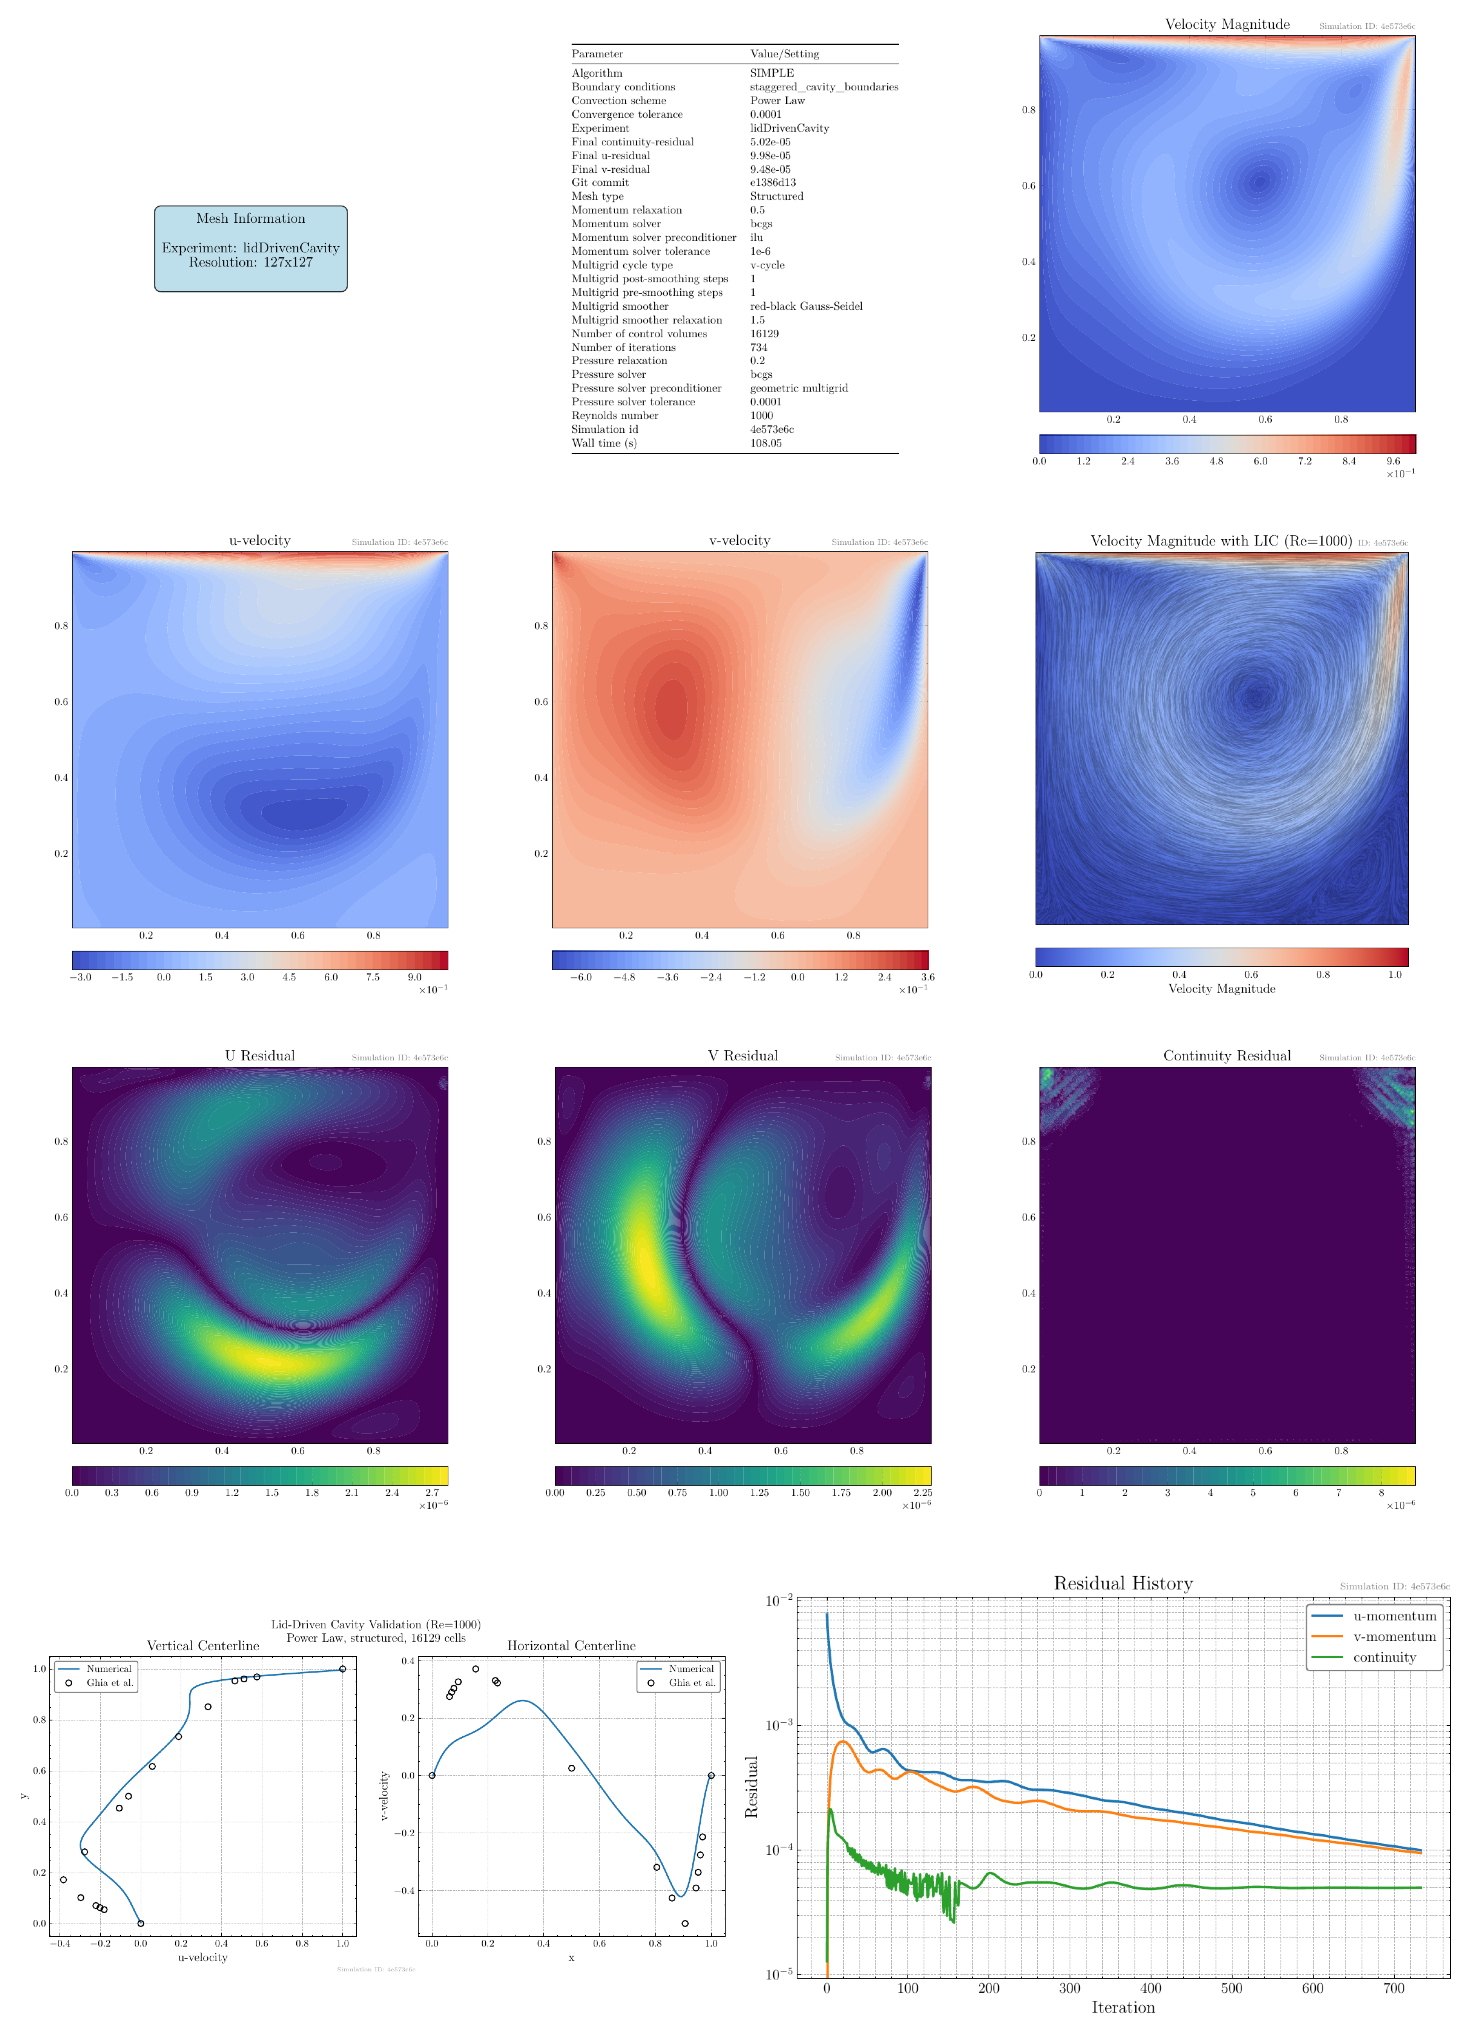
\includegraphics[width=0.85\linewidth]{AppendixPlots/lidDrivenCavity/Re_1000/127x127/lidDrivenCavity_Re1000_structured_127x127_Power Law_4e573e6c.pdf}
    \caption{Liddrivencavity simulation at Re=1000 using structured 127x127 (medium) mesh with Power Law discretization scheme (Simulation ID: 4e573e6c)}
    \label{sim.ldc.re1000.struct.med.powe}
\end{figure}

\begin{figure}[H]
    \centering
    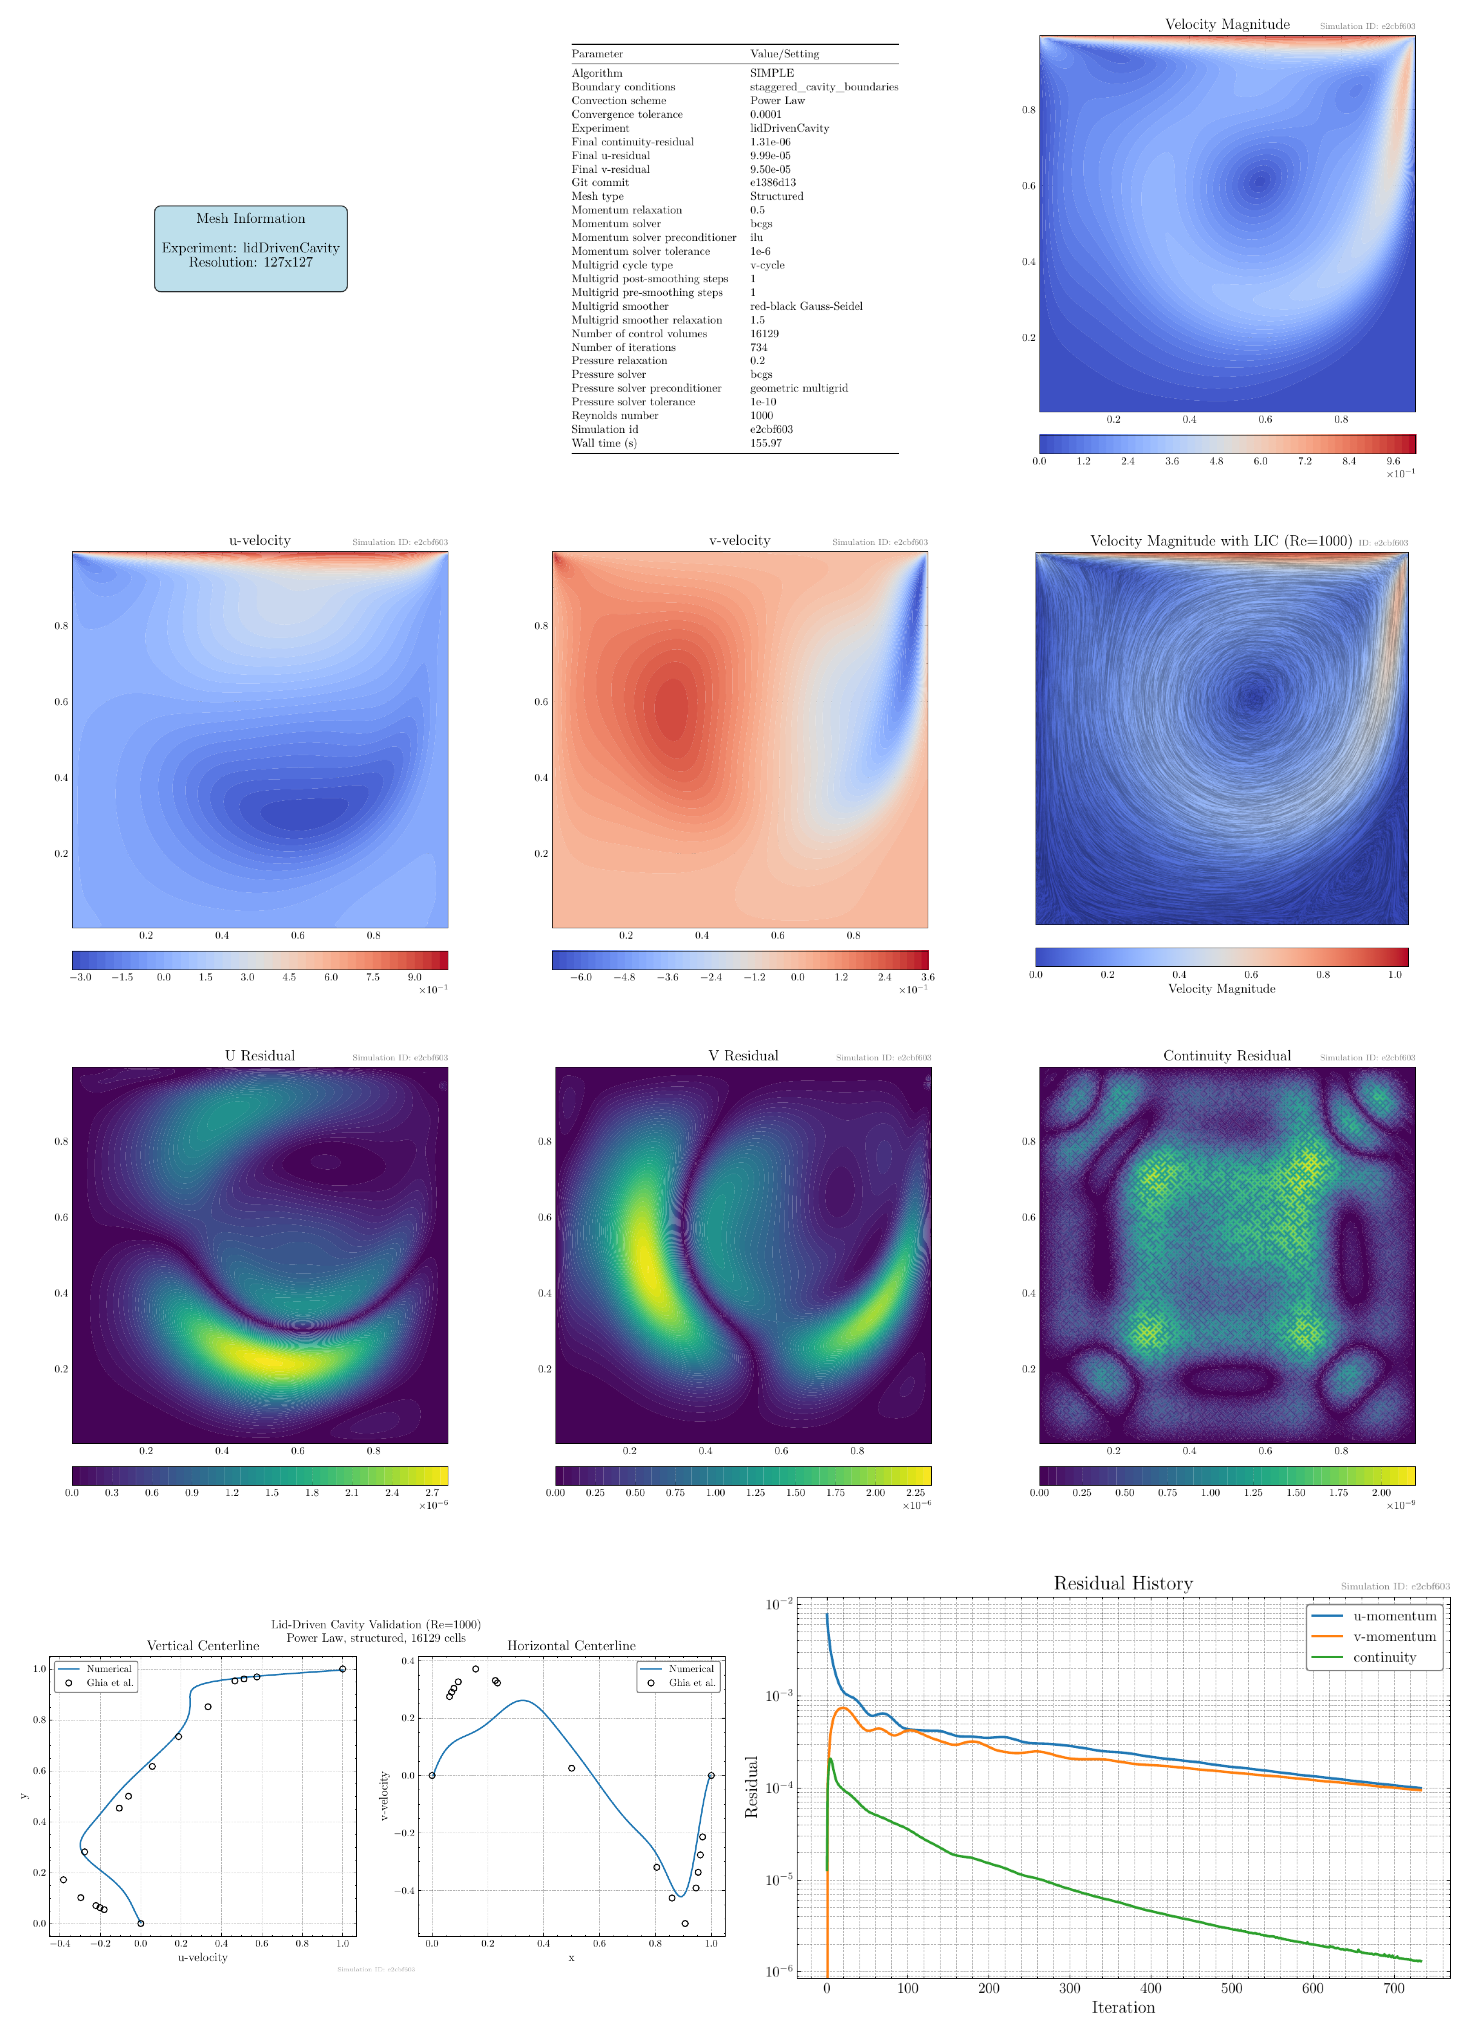
\includegraphics[width=0.85\linewidth]{AppendixPlots/lidDrivenCavity/Re_1000/127x127/lidDrivenCavity_Re1000_structured_127x127_Power Law_e2cbf603.pdf}
    \caption{Liddrivencavity simulation at Re=1000 using structured 127x127 (medium) mesh with Power Law discretization scheme (Simulation ID: e2cbf603)}
    \label{sim.ldc.re1000.struct.med.powe}
\end{figure}

\clearpage

\subsubsection*{63X63 Mesh}
\addcontentsline{toc}{subsubsection}{63X63 Mesh}
\label{subsubsec:liddrivencavity_re1000_63x63}

\paragraph*{Structured Mesh with Power Law Scheme}
\addcontentsline{toc}{paragraph}{Structured Mesh with Power Law Scheme}
\label{para:liddrivencavity_re1000_63x63_structured_Power Law}

\begin{figure}[H]
    \centering
    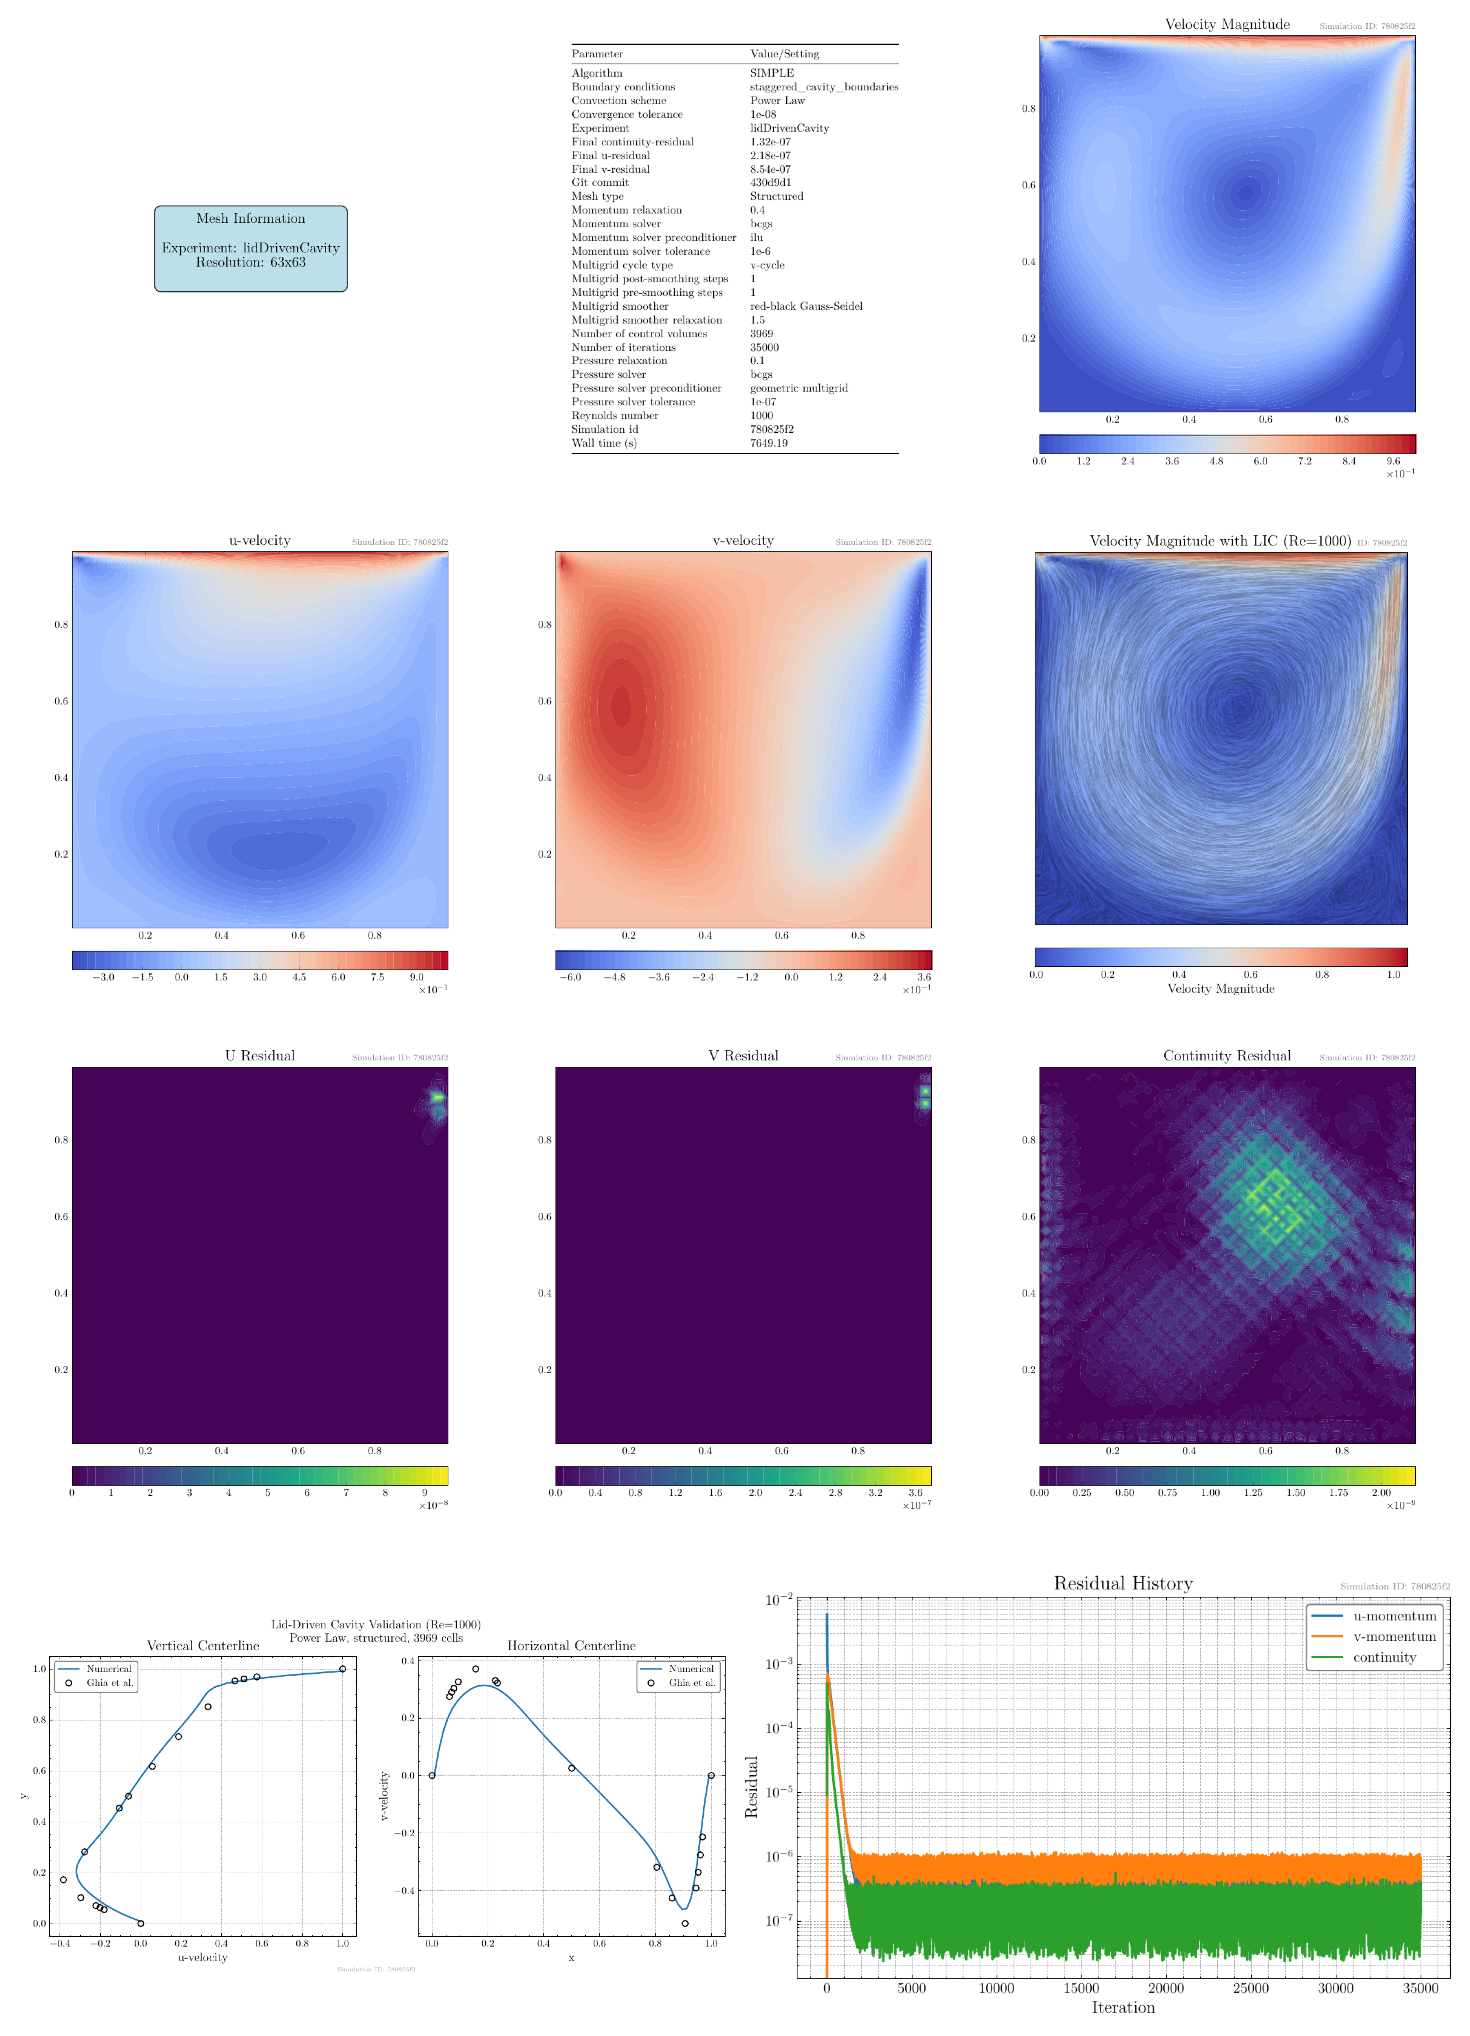
\includegraphics[width=0.85\linewidth]{AppendixPlots/lidDrivenCavity/Re_1000/63x63/lidDrivenCavity_Re1000_structured_63x63_Power Law_780825f2.pdf}
    \caption{Liddrivencavity simulation at Re=1000 using structured 63x63 (coarse) mesh with Power Law discretization scheme (Simulation ID: 780825f2)}
    \label{sim.ldc.re1000.struct.coarse.powe}
\end{figure}

\subsection*{Reynolds Number 3200}
\addcontentsline{toc}{subsection}{Reynolds Number 3200}
\label{subsec:liddrivencavity_re3200}

\subsubsection*{Medium Mesh}
\addcontentsline{toc}{subsubsection}{Medium Mesh}
\label{subsubsec:liddrivencavity_re3200_medium}

\paragraph*{Uniform Mesh with QUICK Scheme}
\addcontentsline{toc}{paragraph}{Uniform Mesh with QUICK Scheme}
\label{para:liddrivencavity_re3200_medium_uniform_QUICK}

\begin{figure}[H]
    \centering
    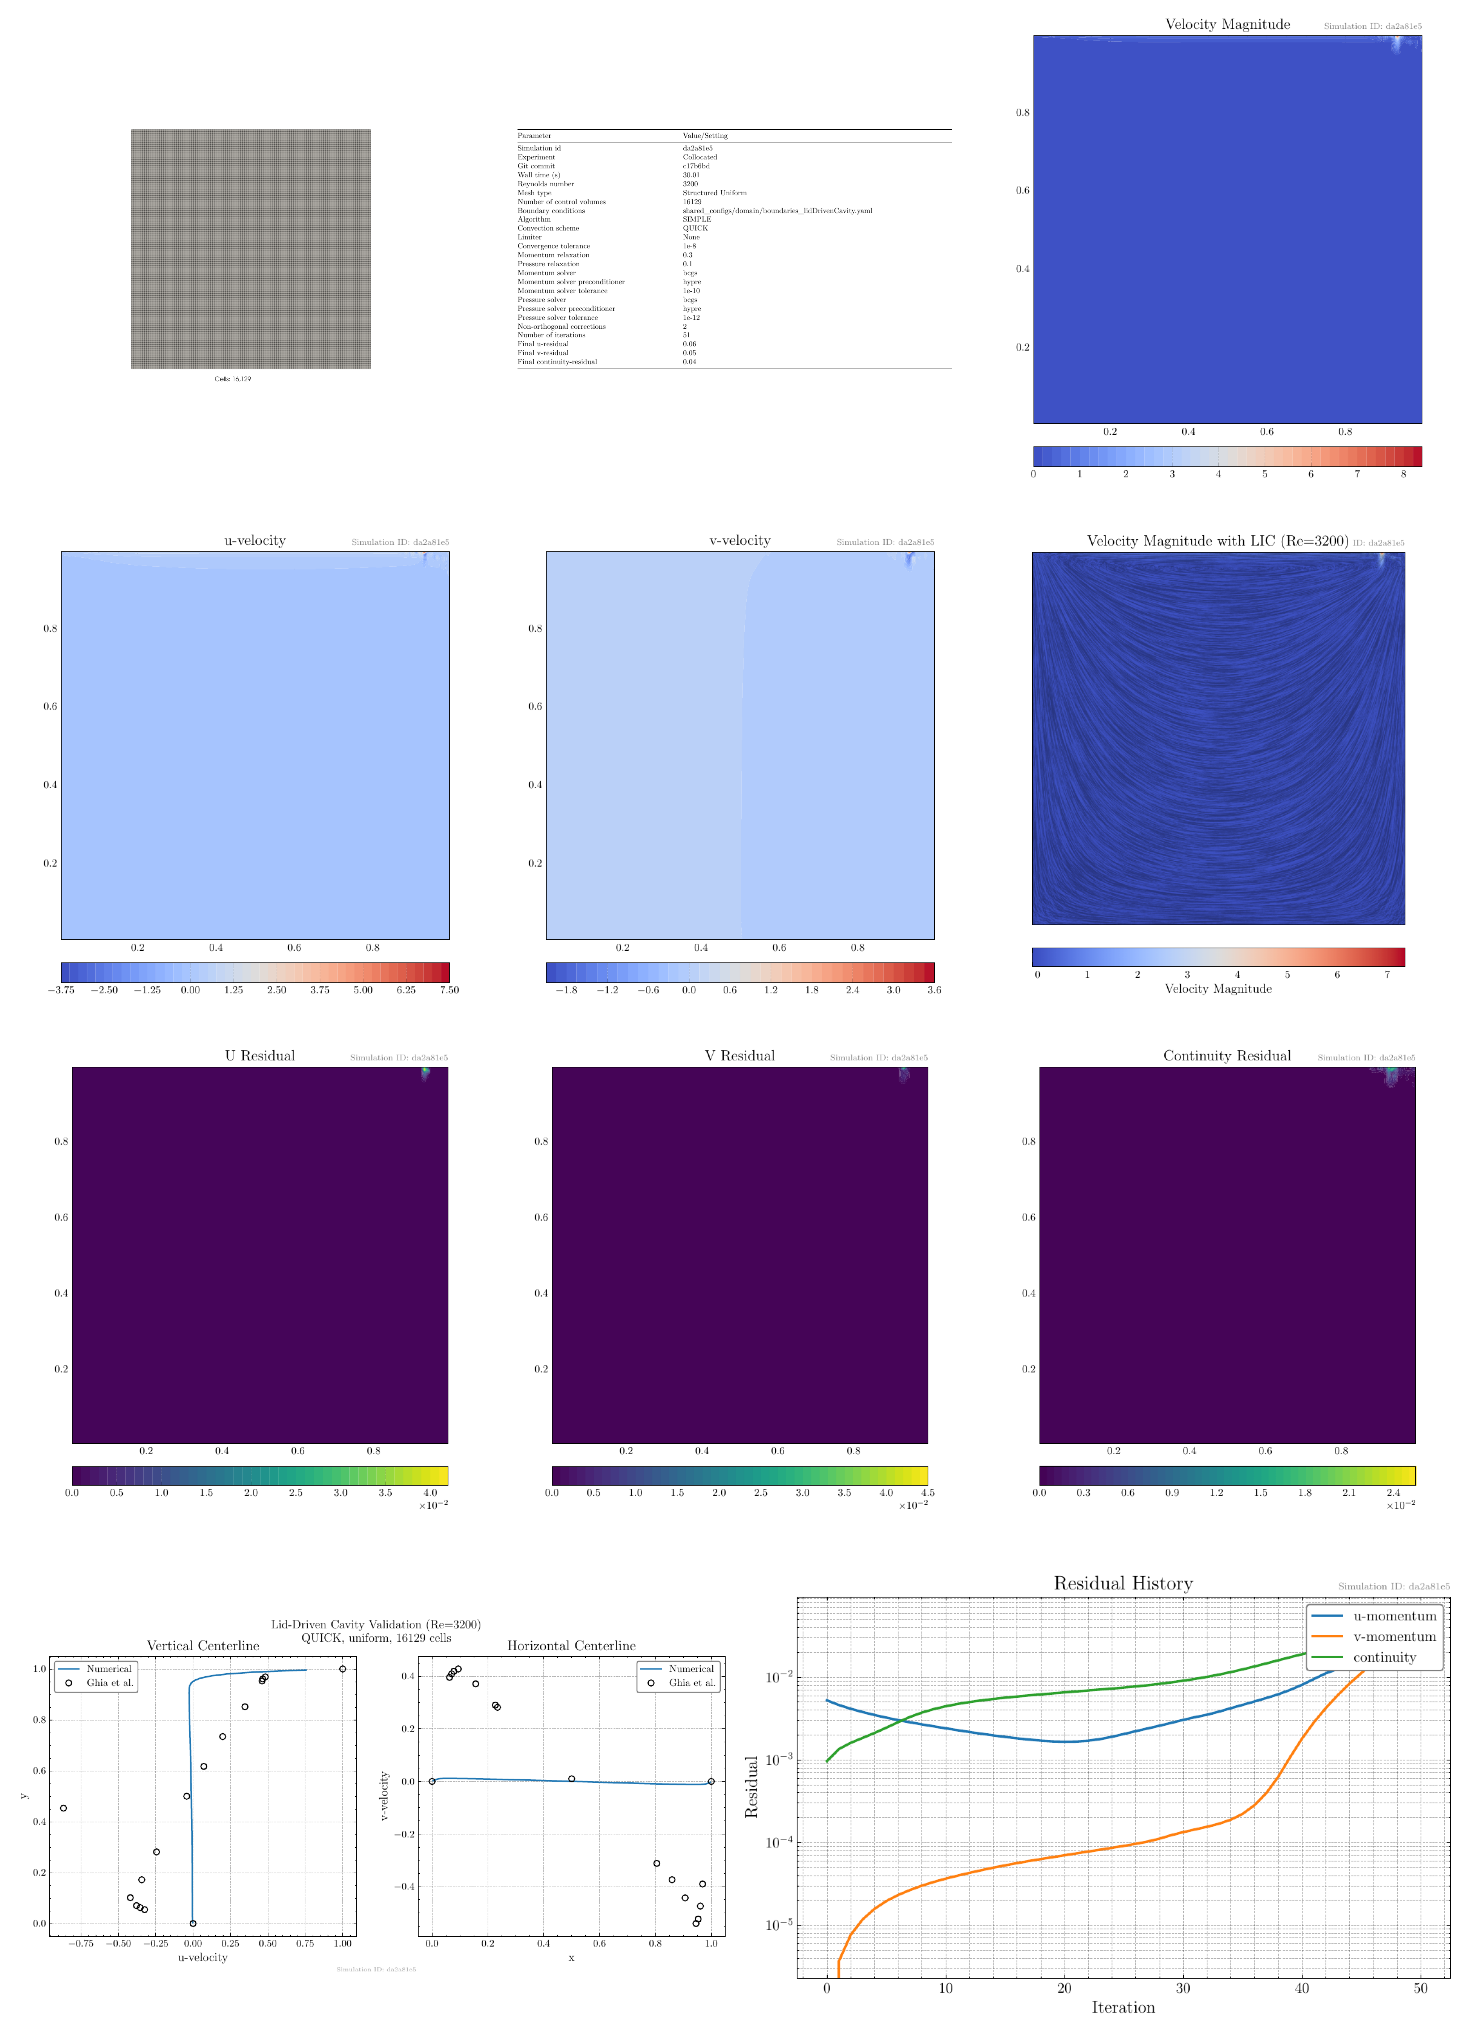
\includegraphics[width=0.85\linewidth]{AppendixPlots/lidDrivenCavity/Re_3200/medium/lidDrivenCavity_Re3200_uniform_medium_QUICK_da2a81e5.pdf}
    \caption{Liddrivencavity simulation at Re=3200 using uniform medium mesh with QUICK discretization scheme (Simulation ID: da2a81e5)}
    \label{sim.ldc.re3200.unif.med.quick}
\end{figure}

\paragraph*{Uniform Mesh with TVD Scheme}
\addcontentsline{toc}{paragraph}{Uniform Mesh with TVD Scheme}
\label{para:liddrivencavity_re3200_medium_uniform_TVD}

\begin{figure}[H]
    \centering
    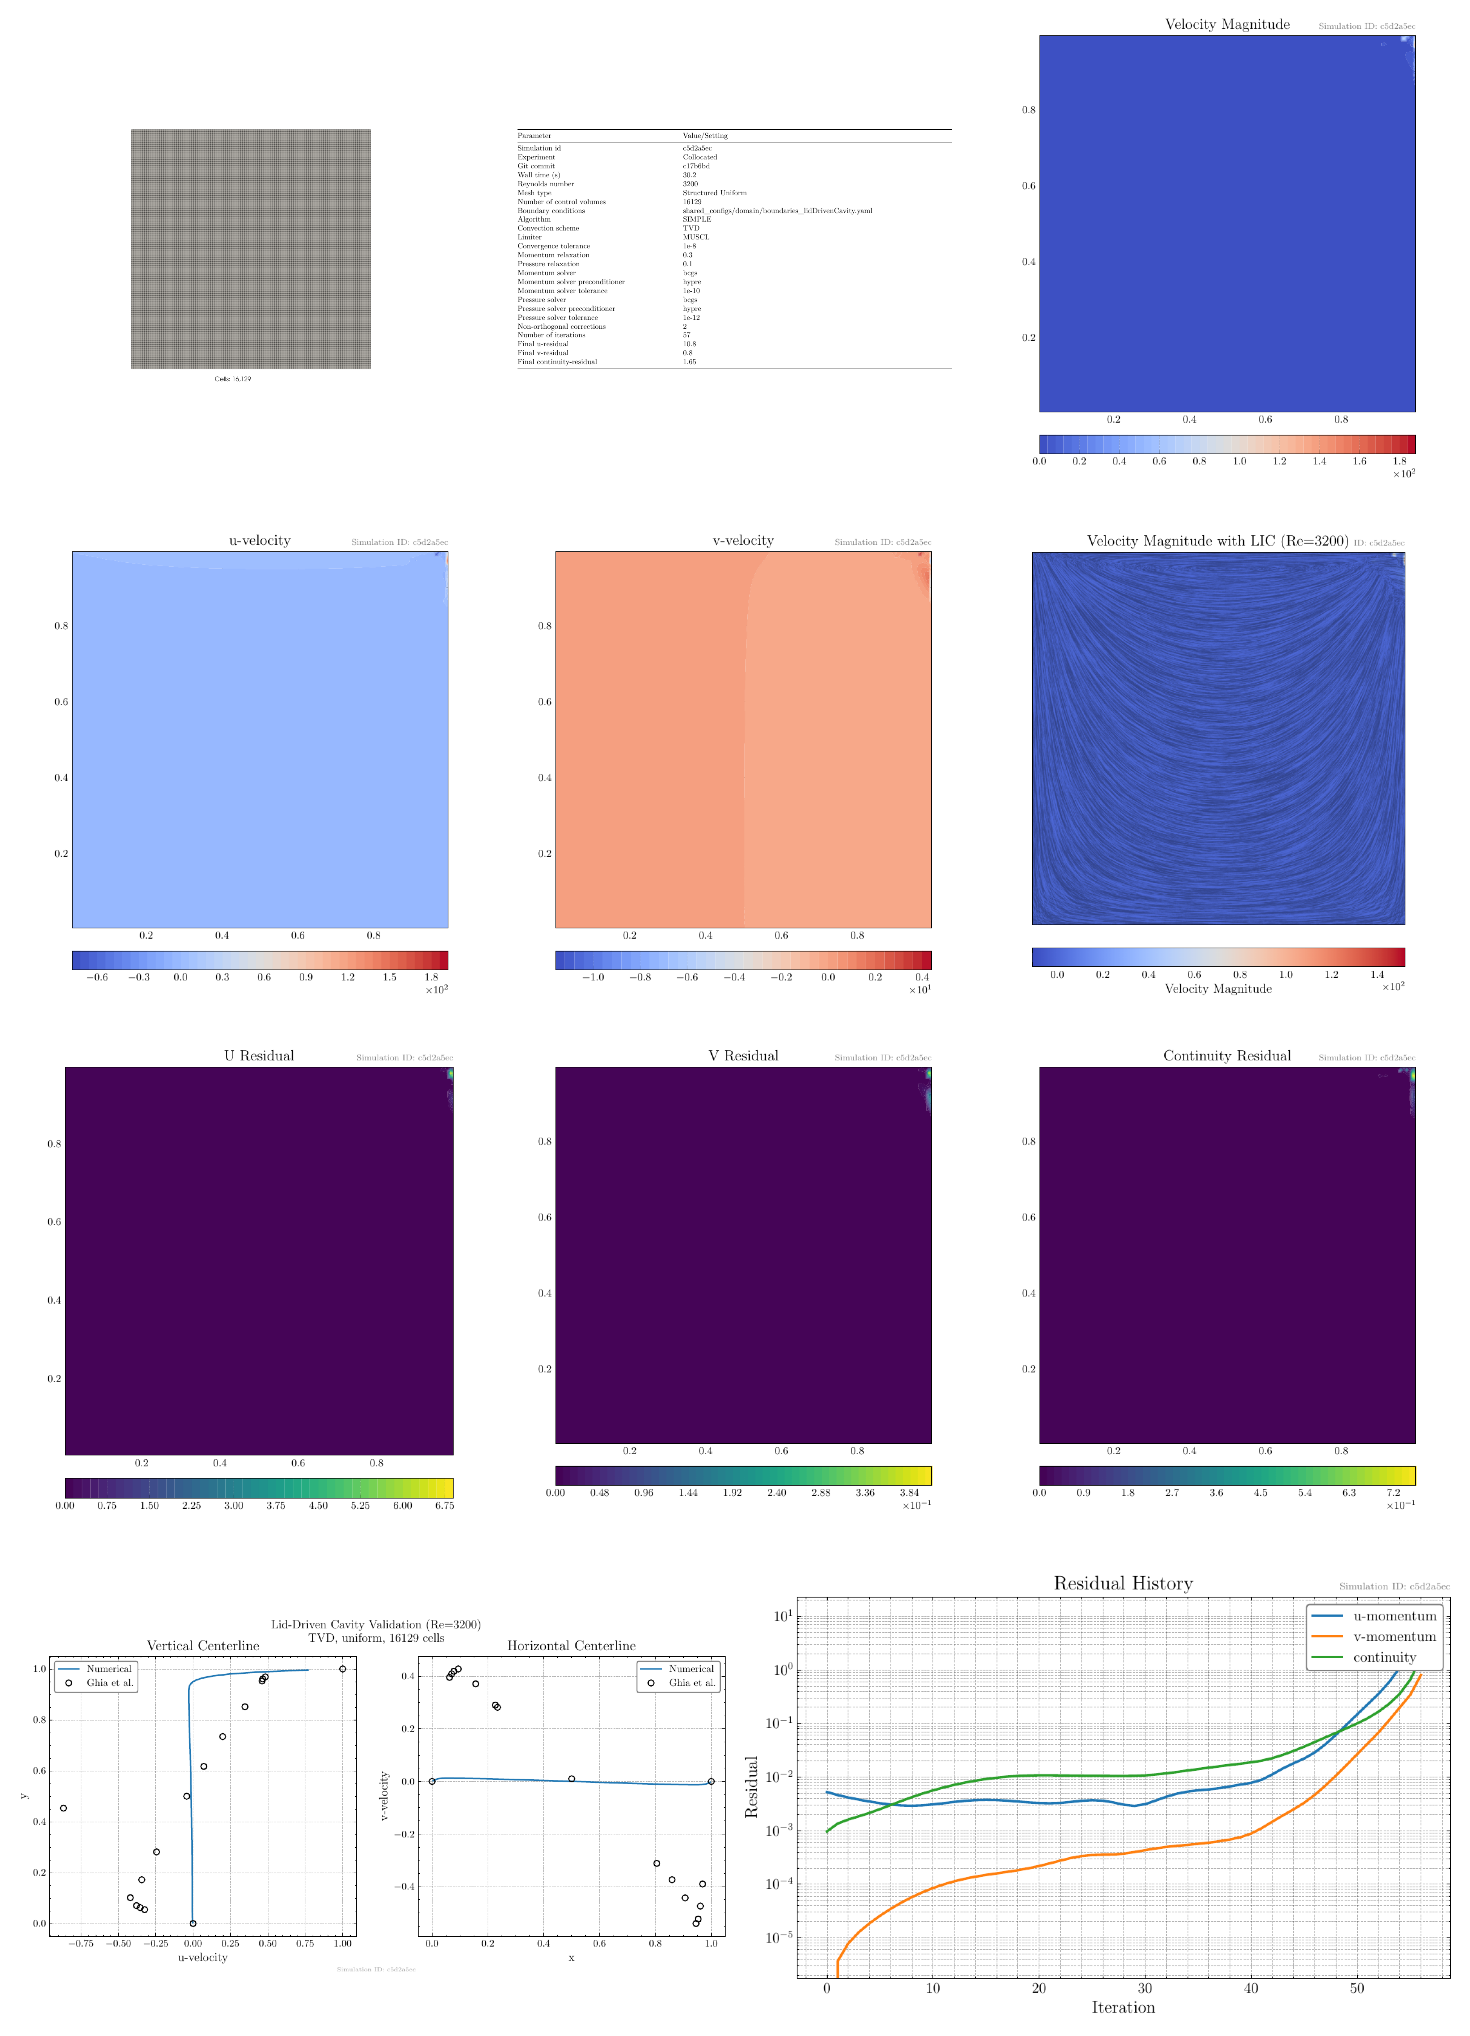
\includegraphics[width=0.85\linewidth]{AppendixPlots/lidDrivenCavity/Re_3200/medium/lidDrivenCavity_Re3200_uniform_medium_TVD_c5d2a5ec.pdf}
    \caption{Liddrivencavity simulation at Re=3200 using uniform medium mesh with TVD discretization scheme (Simulation ID: c5d2a5ec)}
    \label{sim.ldc.re3200.unif.med.tvd}
\end{figure}

\paragraph*{Uniform Mesh with Upwind Scheme}
\addcontentsline{toc}{paragraph}{Uniform Mesh with Upwind Scheme}
\label{para:liddrivencavity_re3200_medium_uniform_Upwind}

\begin{figure}[H]
    \centering
    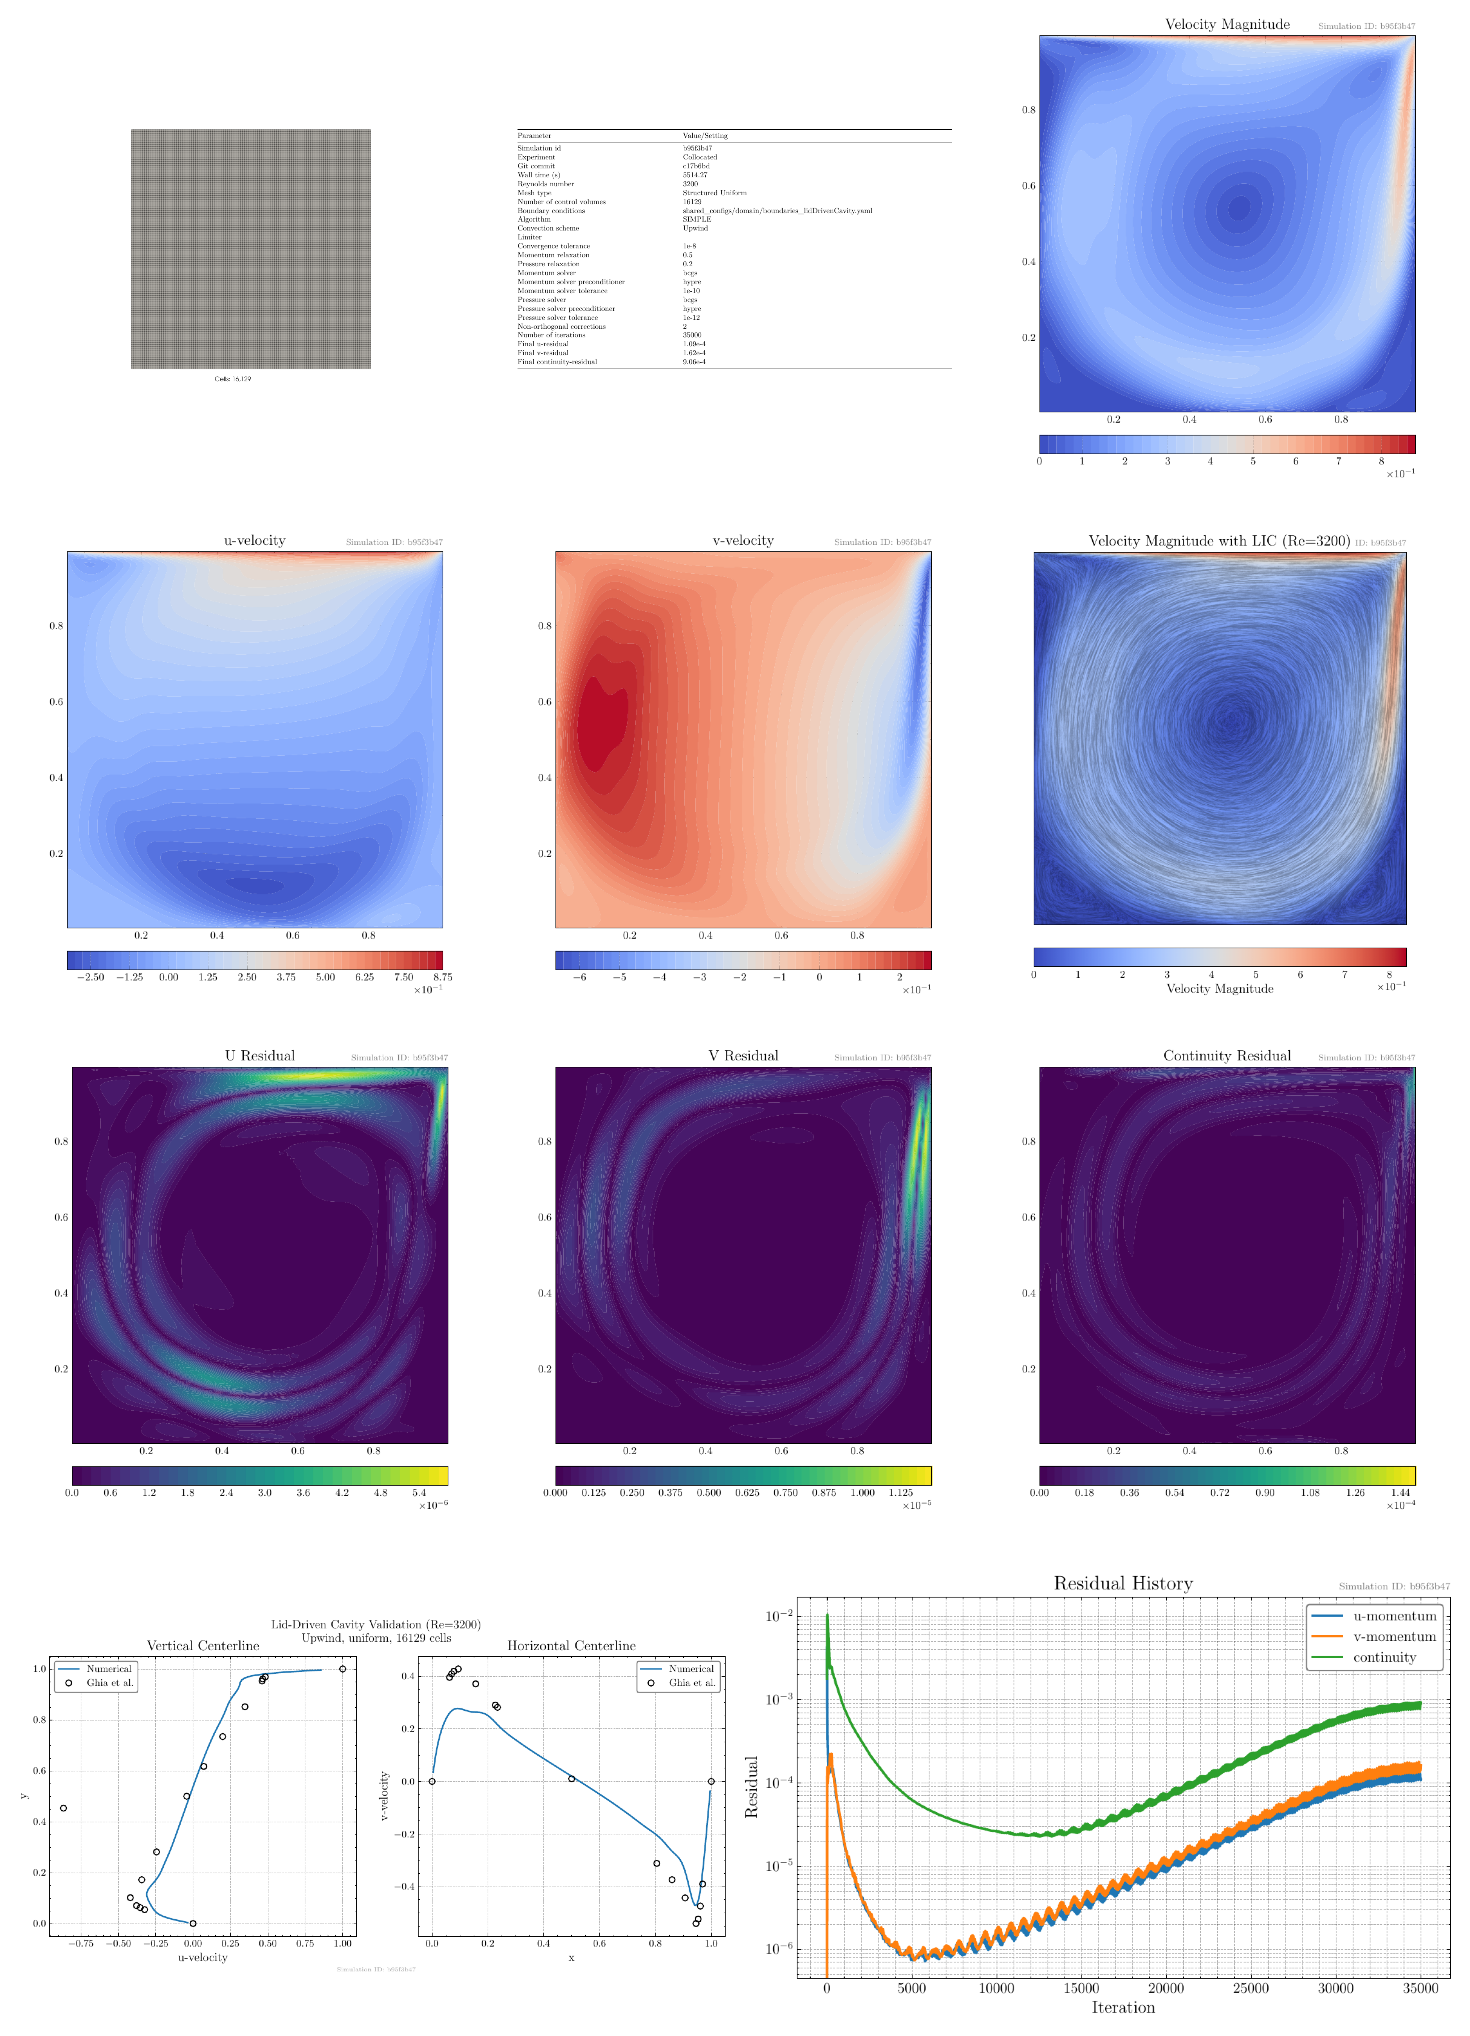
\includegraphics[width=0.85\linewidth]{AppendixPlots/lidDrivenCavity/Re_3200/medium/lidDrivenCavity_Re3200_uniform_medium_Upwind_b95f3b47.pdf}
    \caption{Liddrivencavity simulation at Re=3200 using uniform medium mesh with Upwind discretization scheme (Simulation ID: b95f3b47)}
    \label{sim.ldc.re3200.unif.med.upwind}
\end{figure}

\paragraph*{Unstructured Mesh with Upwind Scheme}
\addcontentsline{toc}{paragraph}{Unstructured Mesh with Upwind Scheme}
\label{para:liddrivencavity_re3200_medium_unstructured_Upwind}

\begin{figure}[H]
    \centering
    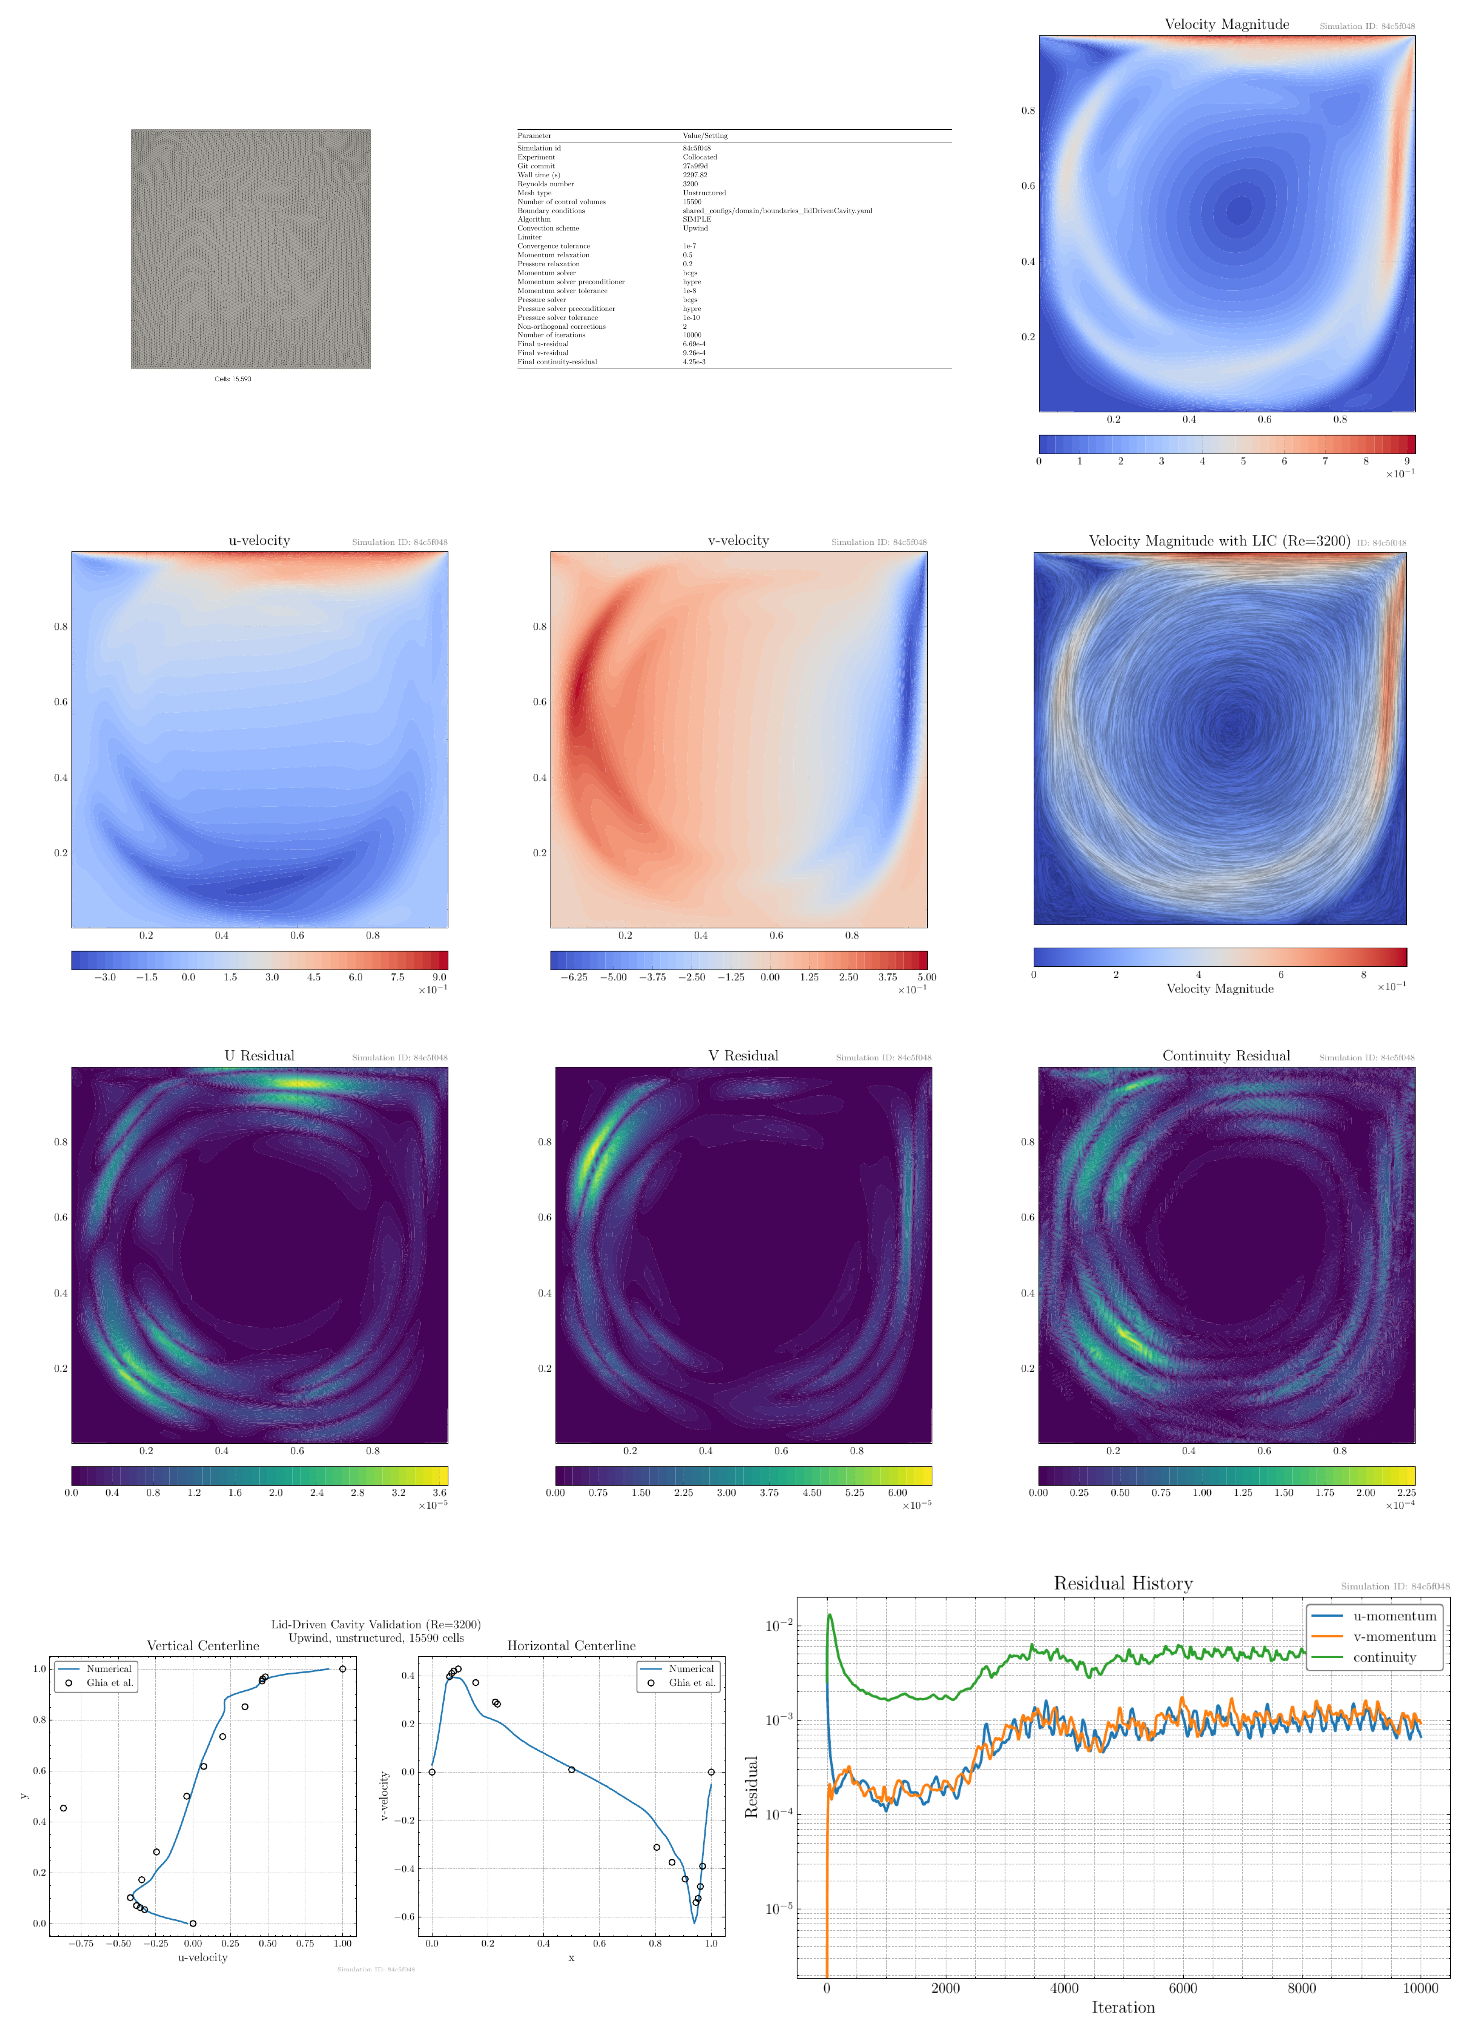
\includegraphics[width=0.85\linewidth]{AppendixPlots/lidDrivenCavity/Re_3200/medium/lidDrivenCavity_Re3200_unstructured_medium_Upwind_84c5f048.pdf}
    \caption{Liddrivencavity simulation at Re=3200 using unstructured medium mesh with Upwind discretization scheme (Simulation ID: 84c5f048)}
    \label{sim.ldc.re3200.unstruct.med.upwind}
\end{figure}

\clearpage

\subsubsection*{Fine Mesh}
\addcontentsline{toc}{subsubsection}{Fine Mesh}
\label{subsubsec:liddrivencavity_re3200_fine}

\paragraph*{Uniform Mesh with TVD Scheme}
\addcontentsline{toc}{paragraph}{Uniform Mesh with TVD Scheme}
\label{para:liddrivencavity_re3200_fine_uniform_TVD}

\begin{figure}[H]
    \centering
    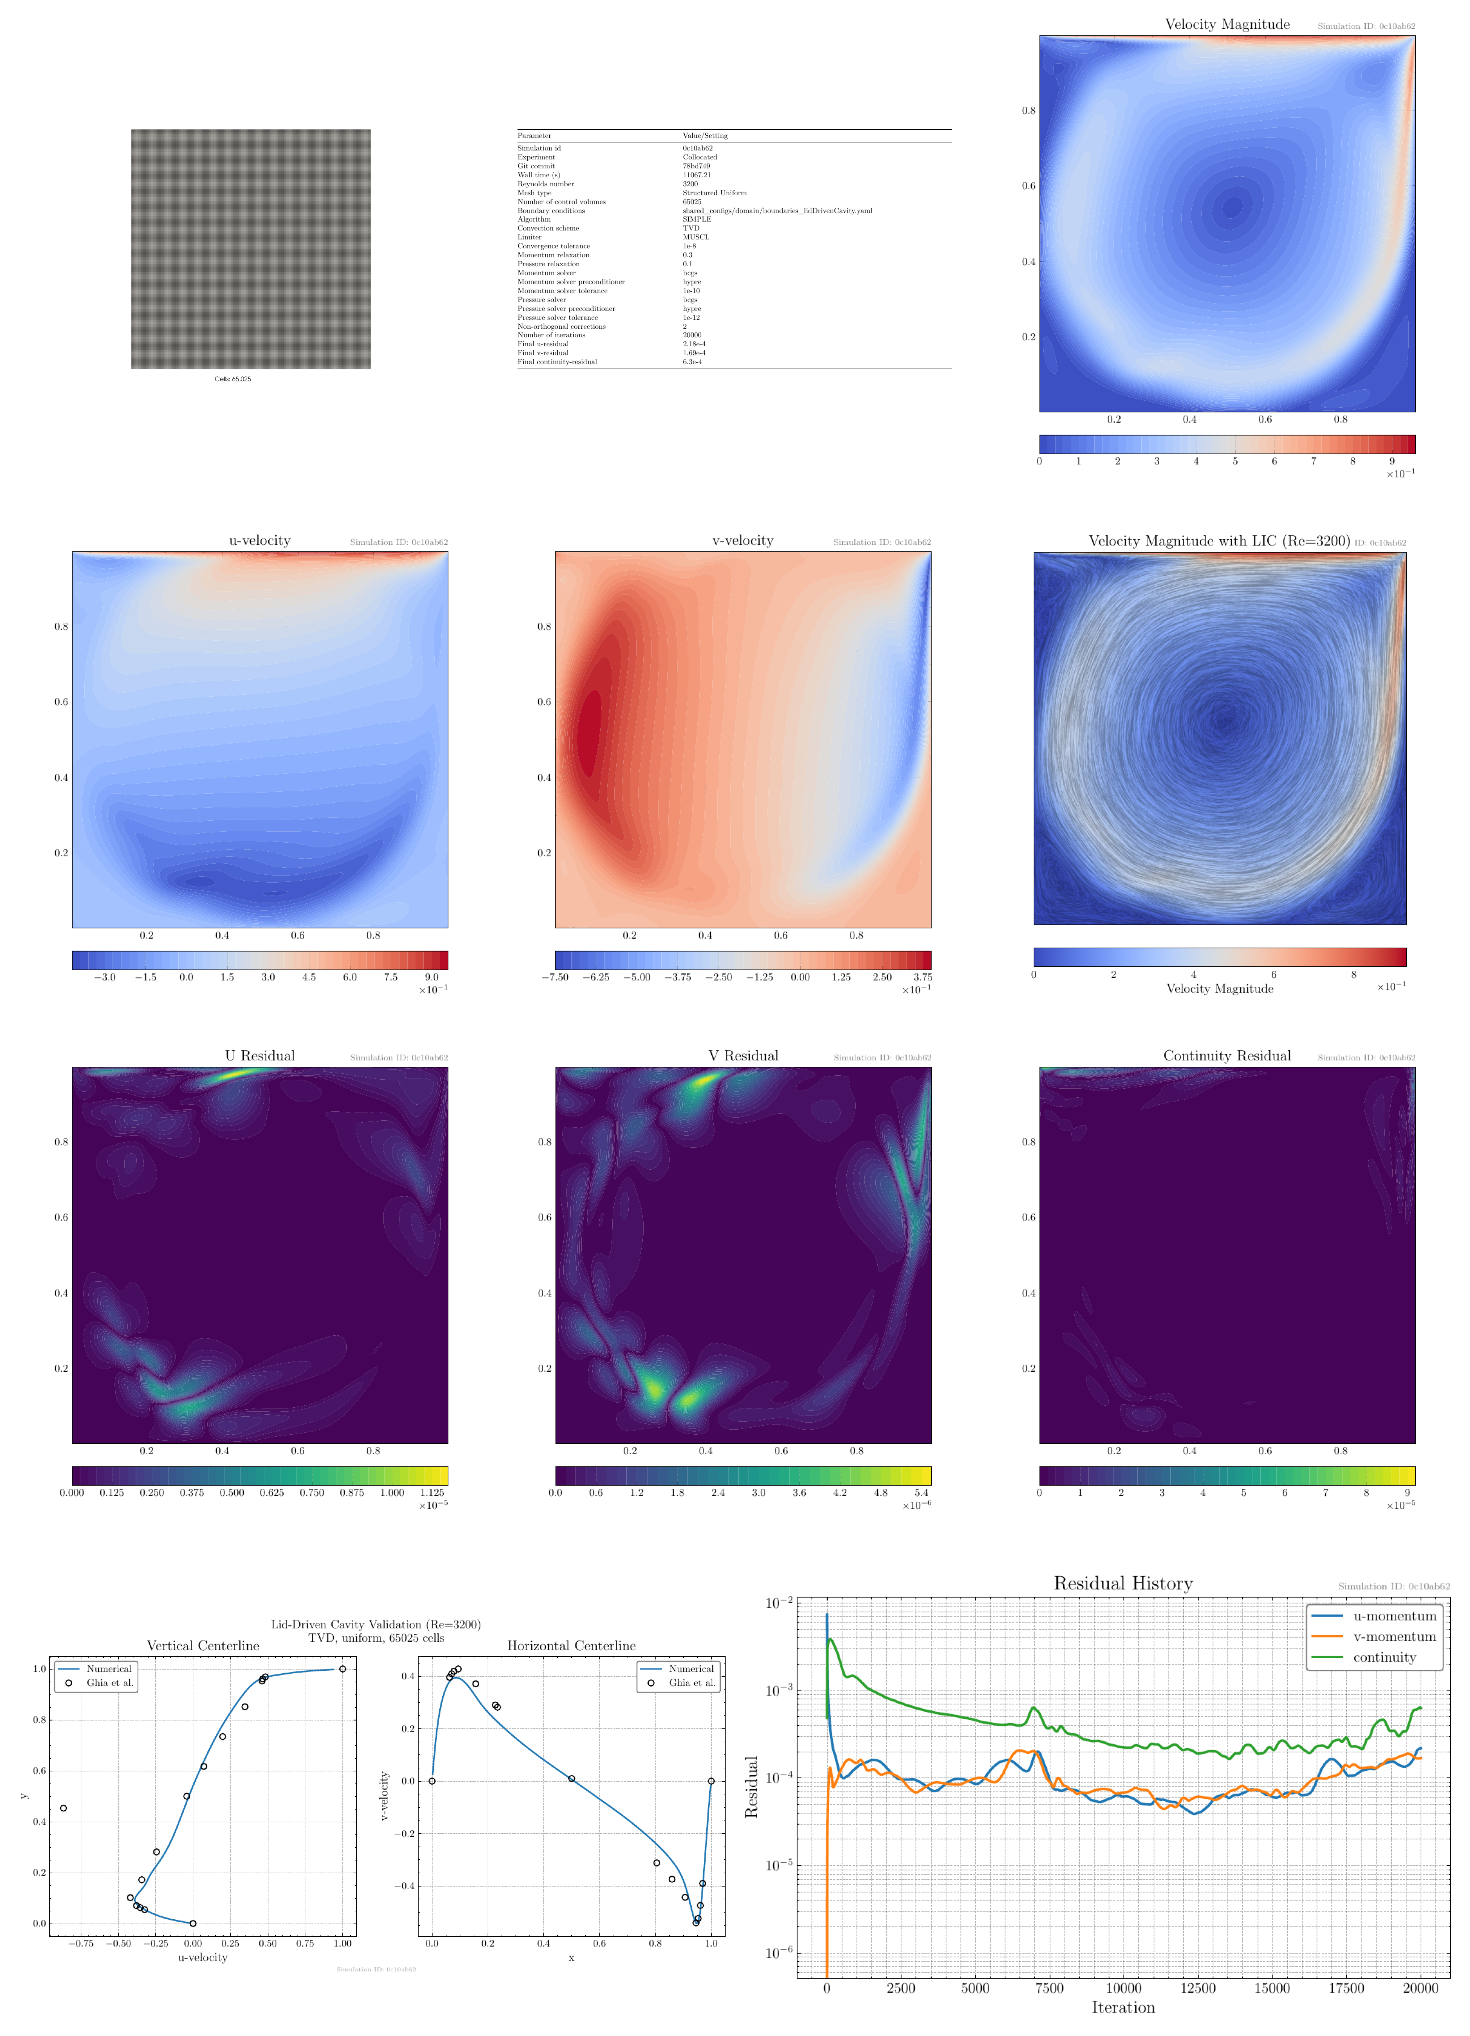
\includegraphics[width=0.85\linewidth]{AppendixPlots/lidDrivenCavity/Re_3200/fine/lidDrivenCavity_Re3200_uniform_fine_TVD_0c10ab62.pdf}
    \caption{Liddrivencavity simulation at Re=3200 using uniform fine mesh with TVD discretization scheme (Simulation ID: 0c10ab62)}
    \label{sim.ldc.re3200.unif.fine.tvd}
\end{figure}

\paragraph*{Uniform Mesh with Upwind Scheme}
\addcontentsline{toc}{paragraph}{Uniform Mesh with Upwind Scheme}
\label{para:liddrivencavity_re3200_fine_uniform_Upwind}

\begin{figure}[H]
    \centering
    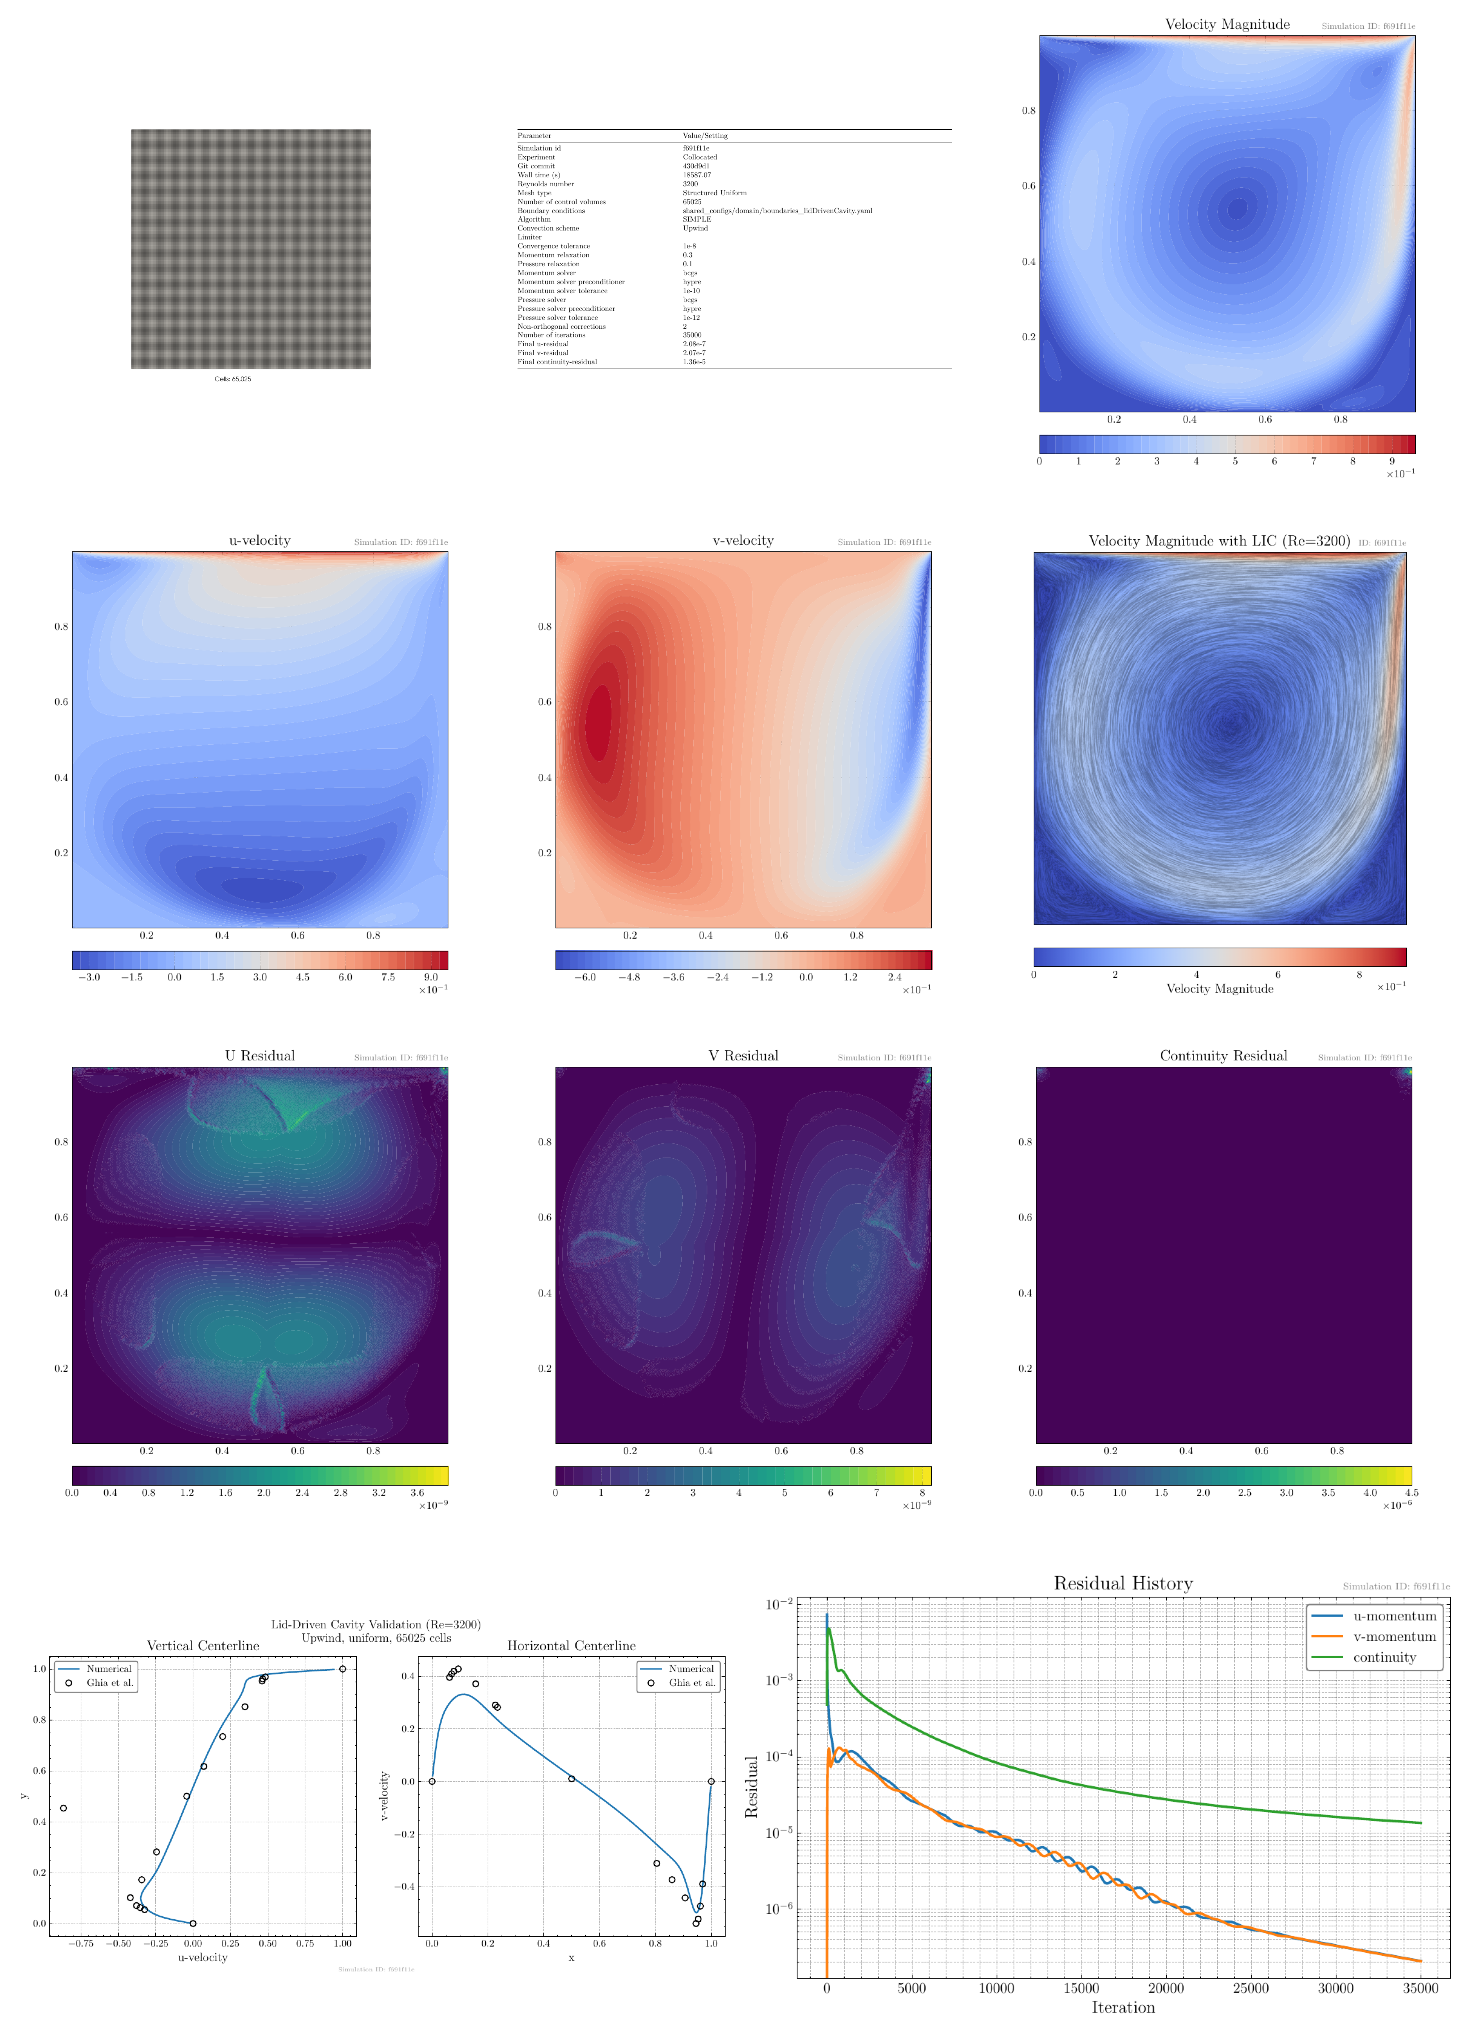
\includegraphics[width=0.85\linewidth]{AppendixPlots/lidDrivenCavity/Re_3200/fine/lidDrivenCavity_Re3200_uniform_fine_Upwind_f691f11e.pdf}
    \caption{Liddrivencavity simulation at Re=3200 using uniform fine mesh with Upwind discretization scheme (Simulation ID: f691f11e)}
    \label{sim.ldc.re3200.unif.fine.upwind}
\end{figure}

\paragraph*{Unstructured Mesh with Upwind Scheme}
\addcontentsline{toc}{paragraph}{Unstructured Mesh with Upwind Scheme}
\label{para:liddrivencavity_re3200_fine_unstructured_Upwind}

\begin{figure}[H]
    \centering
    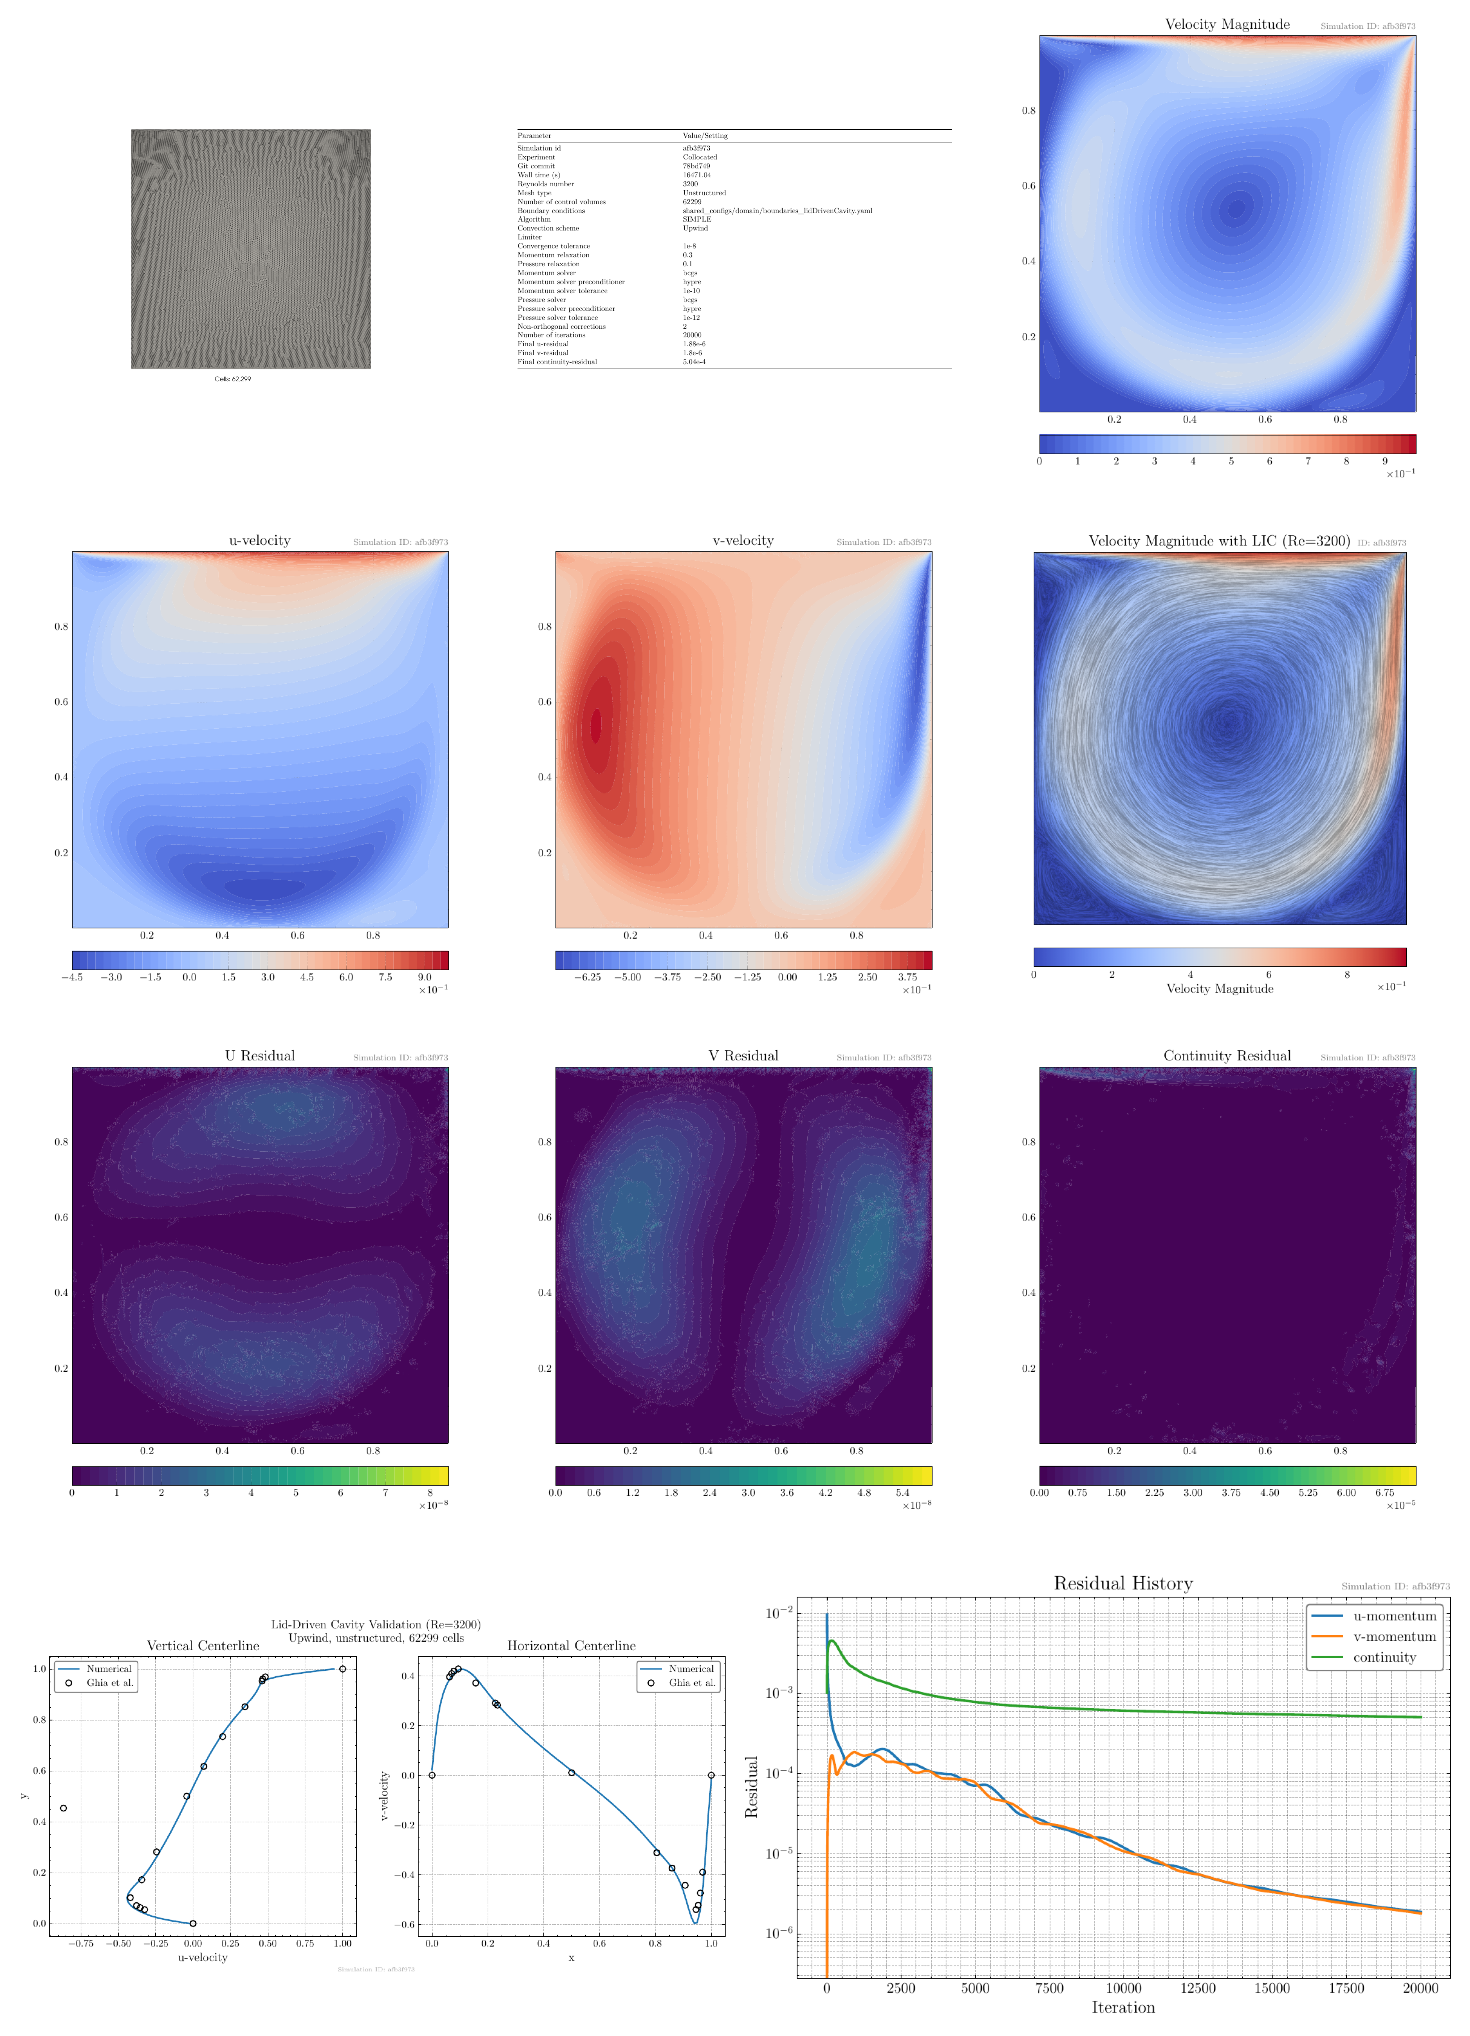
\includegraphics[width=0.85\linewidth]{AppendixPlots/lidDrivenCavity/Re_3200/fine/lidDrivenCavity_Re3200_unstructured_fine_Upwind_afb3f973.pdf}
    \caption{Liddrivencavity simulation at Re=3200 using unstructured fine mesh with Upwind discretization scheme (Simulation ID: afb3f973)}
    \label{sim.ldc.re3200.unstruct.fine.upwind}
\end{figure}

\clearpage

\subsubsection*{127X127 Mesh}
\addcontentsline{toc}{subsubsection}{127X127 Mesh}
\label{subsubsec:liddrivencavity_re3200_127x127}

\paragraph*{Structured Mesh with Power Law Scheme}
\addcontentsline{toc}{paragraph}{Structured Mesh with Power Law Scheme}
\label{para:liddrivencavity_re3200_127x127_structured_Power Law}

\begin{figure}[H]
    \centering
    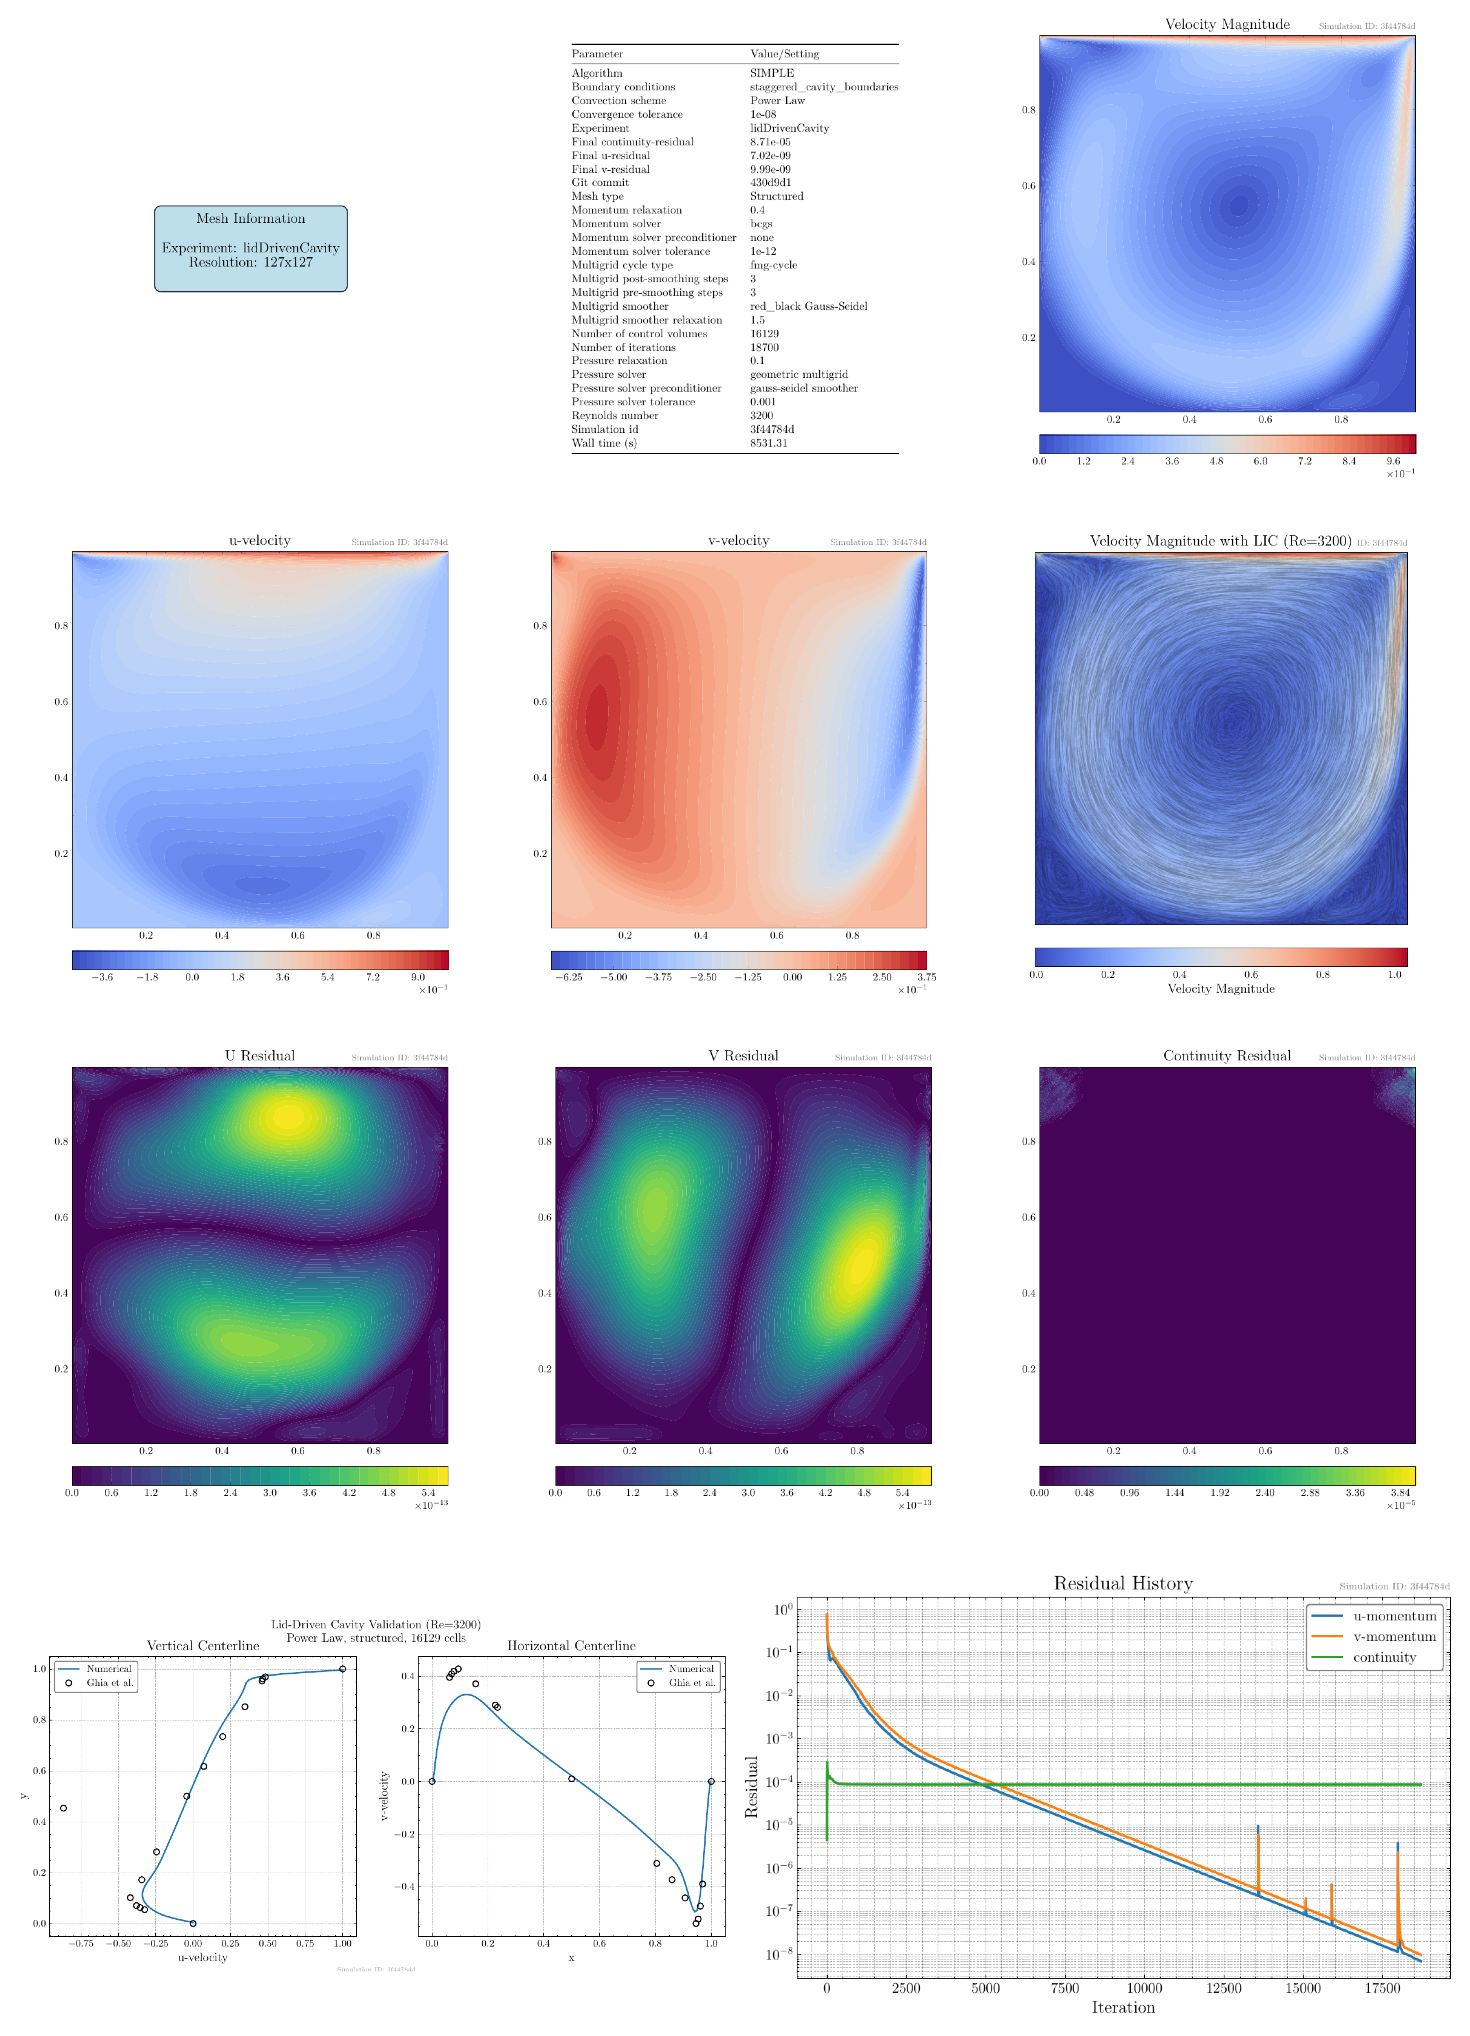
\includegraphics[width=0.85\linewidth]{AppendixPlots/lidDrivenCavity/Re_3200/127x127/lidDrivenCavity_Re3200_structured_127x127_Power Law_3f44784d.pdf}
    \caption{Liddrivencavity simulation at Re=3200 using structured 127x127 (medium) mesh with Power Law discretization scheme with FMG (Simulation ID: 3f44784d)}
    \label{sim.ldc.re3200.struct.med.powe}
\end{figure}

\begin{figure}[H]
    \centering
    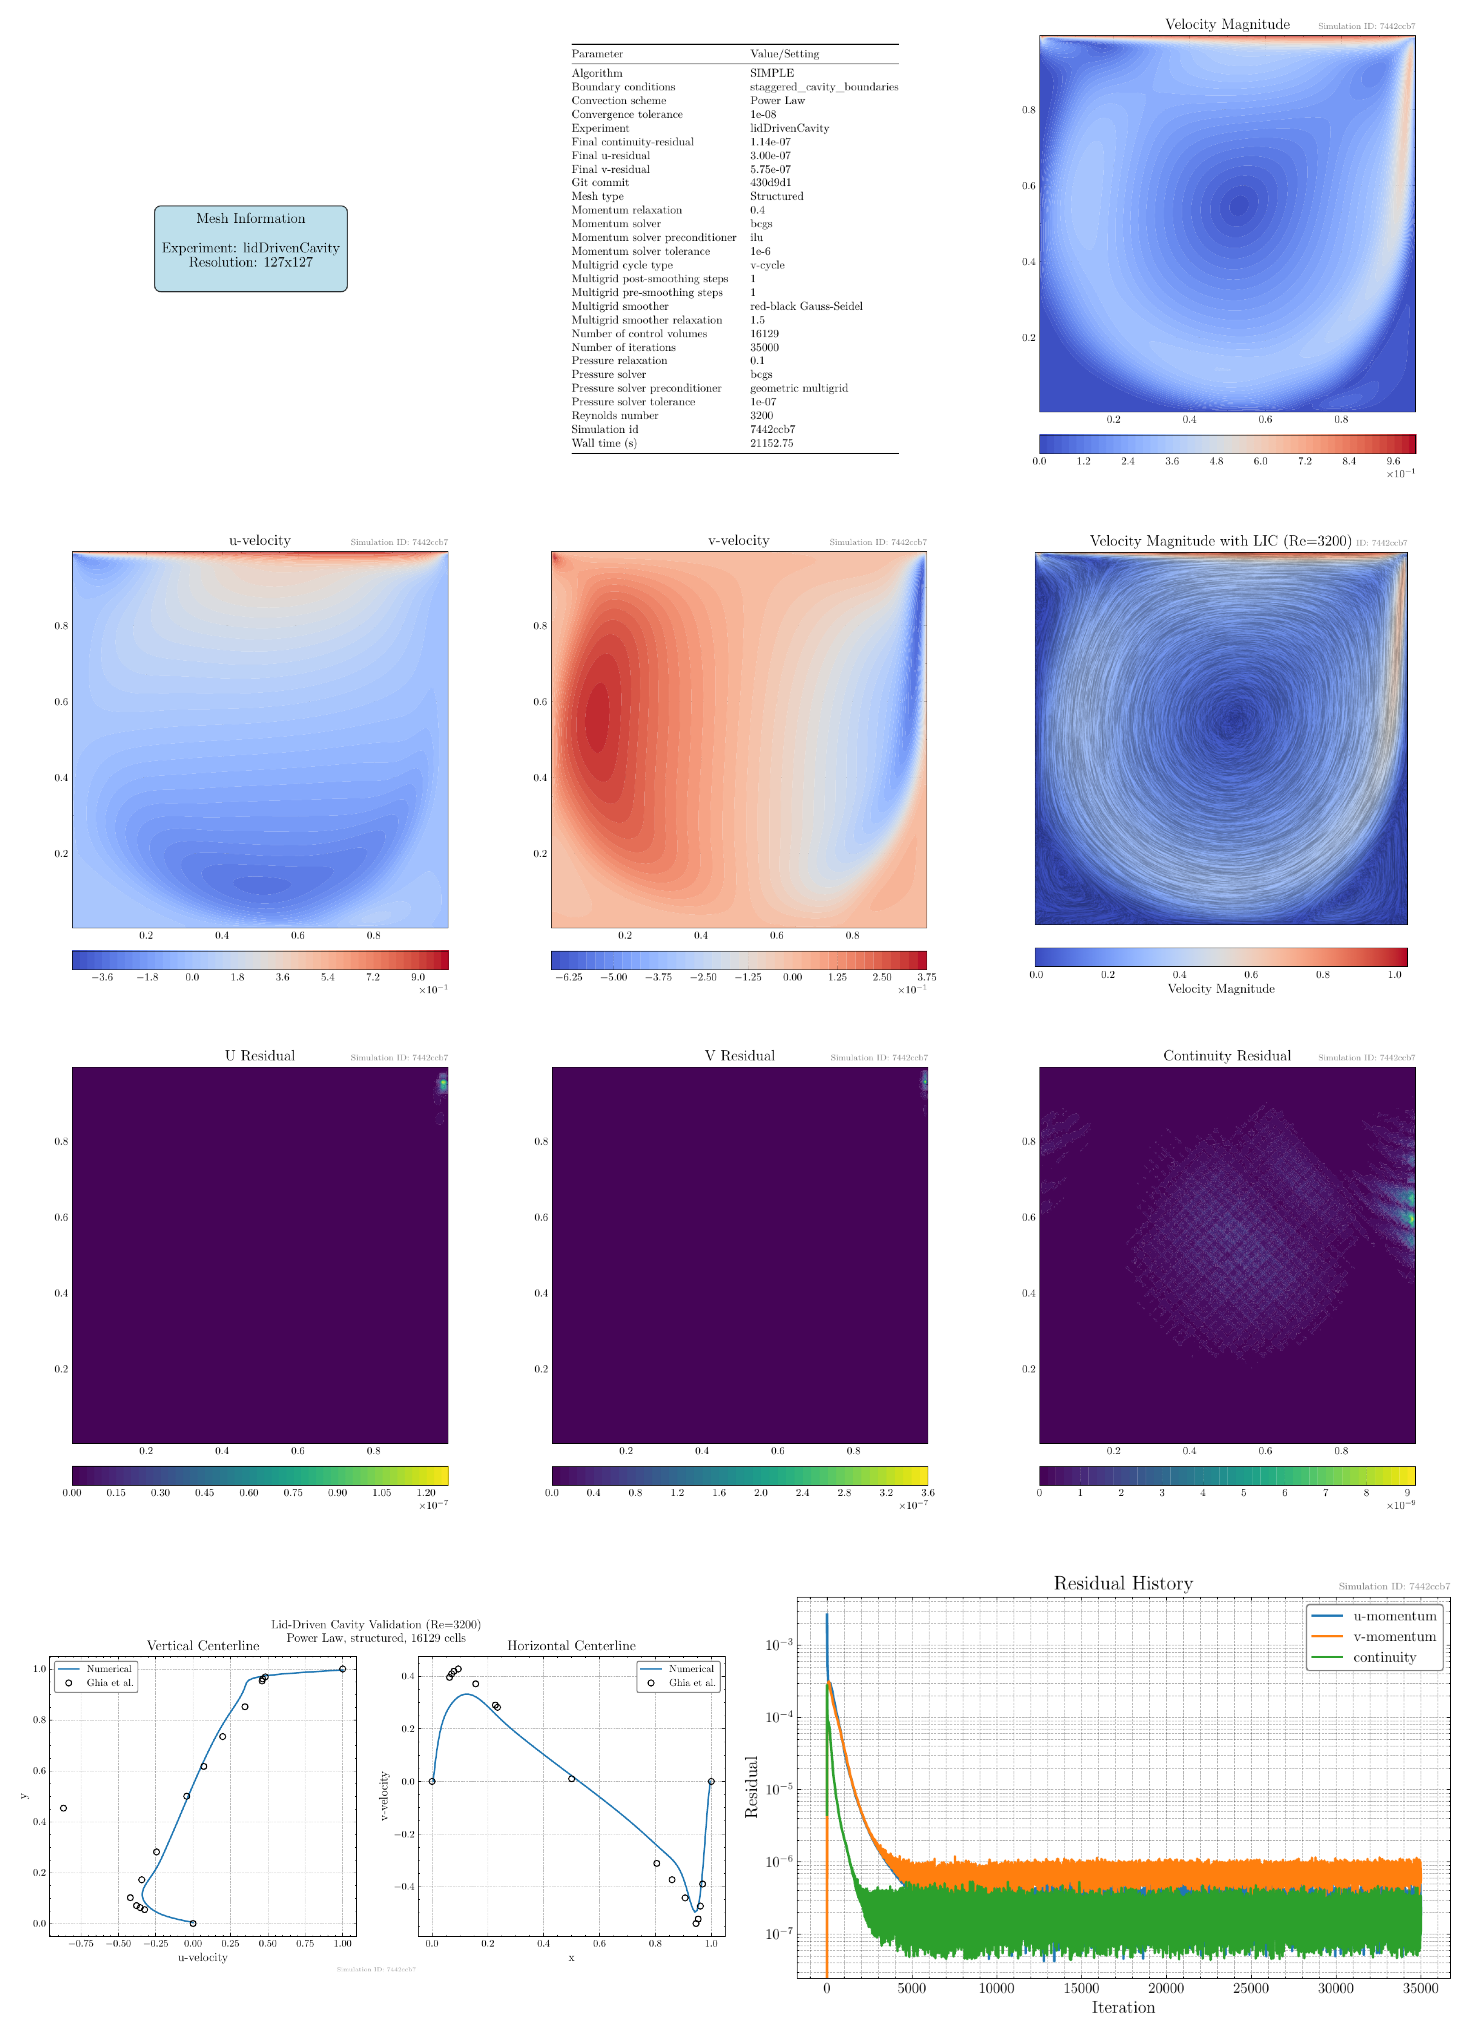
\includegraphics[width=0.85\linewidth]{AppendixPlots/lidDrivenCavity/Re_3200/127x127/lidDrivenCavity_Re3200_structured_127x127_Power Law_7442ccb7.pdf}
    \caption{Liddrivencavity simulation at Re=3200 using structured 127x127 (medium) mesh with Power Law discretization scheme with FMG (Simulation ID: 7442ccb7)}
    \label{sim.ldc.re3200.struct.med.powe}
\end{figure}

\subsection*{Reynolds Number 5000}
\addcontentsline{toc}{subsection}{Reynolds Number 5000}
\label{subsec:liddrivencavity_re5000}

\subsubsection*{Medium Mesh}
\addcontentsline{toc}{subsubsection}{Medium Mesh}
\label{subsubsec:liddrivencavity_re5000_medium}

\paragraph*{Uniform Mesh with QUICK Scheme}
\addcontentsline{toc}{paragraph}{Uniform Mesh with QUICK Scheme}
\label{para:liddrivencavity_re5000_medium_uniform_QUICK}

\begin{figure}[H]
    \centering
    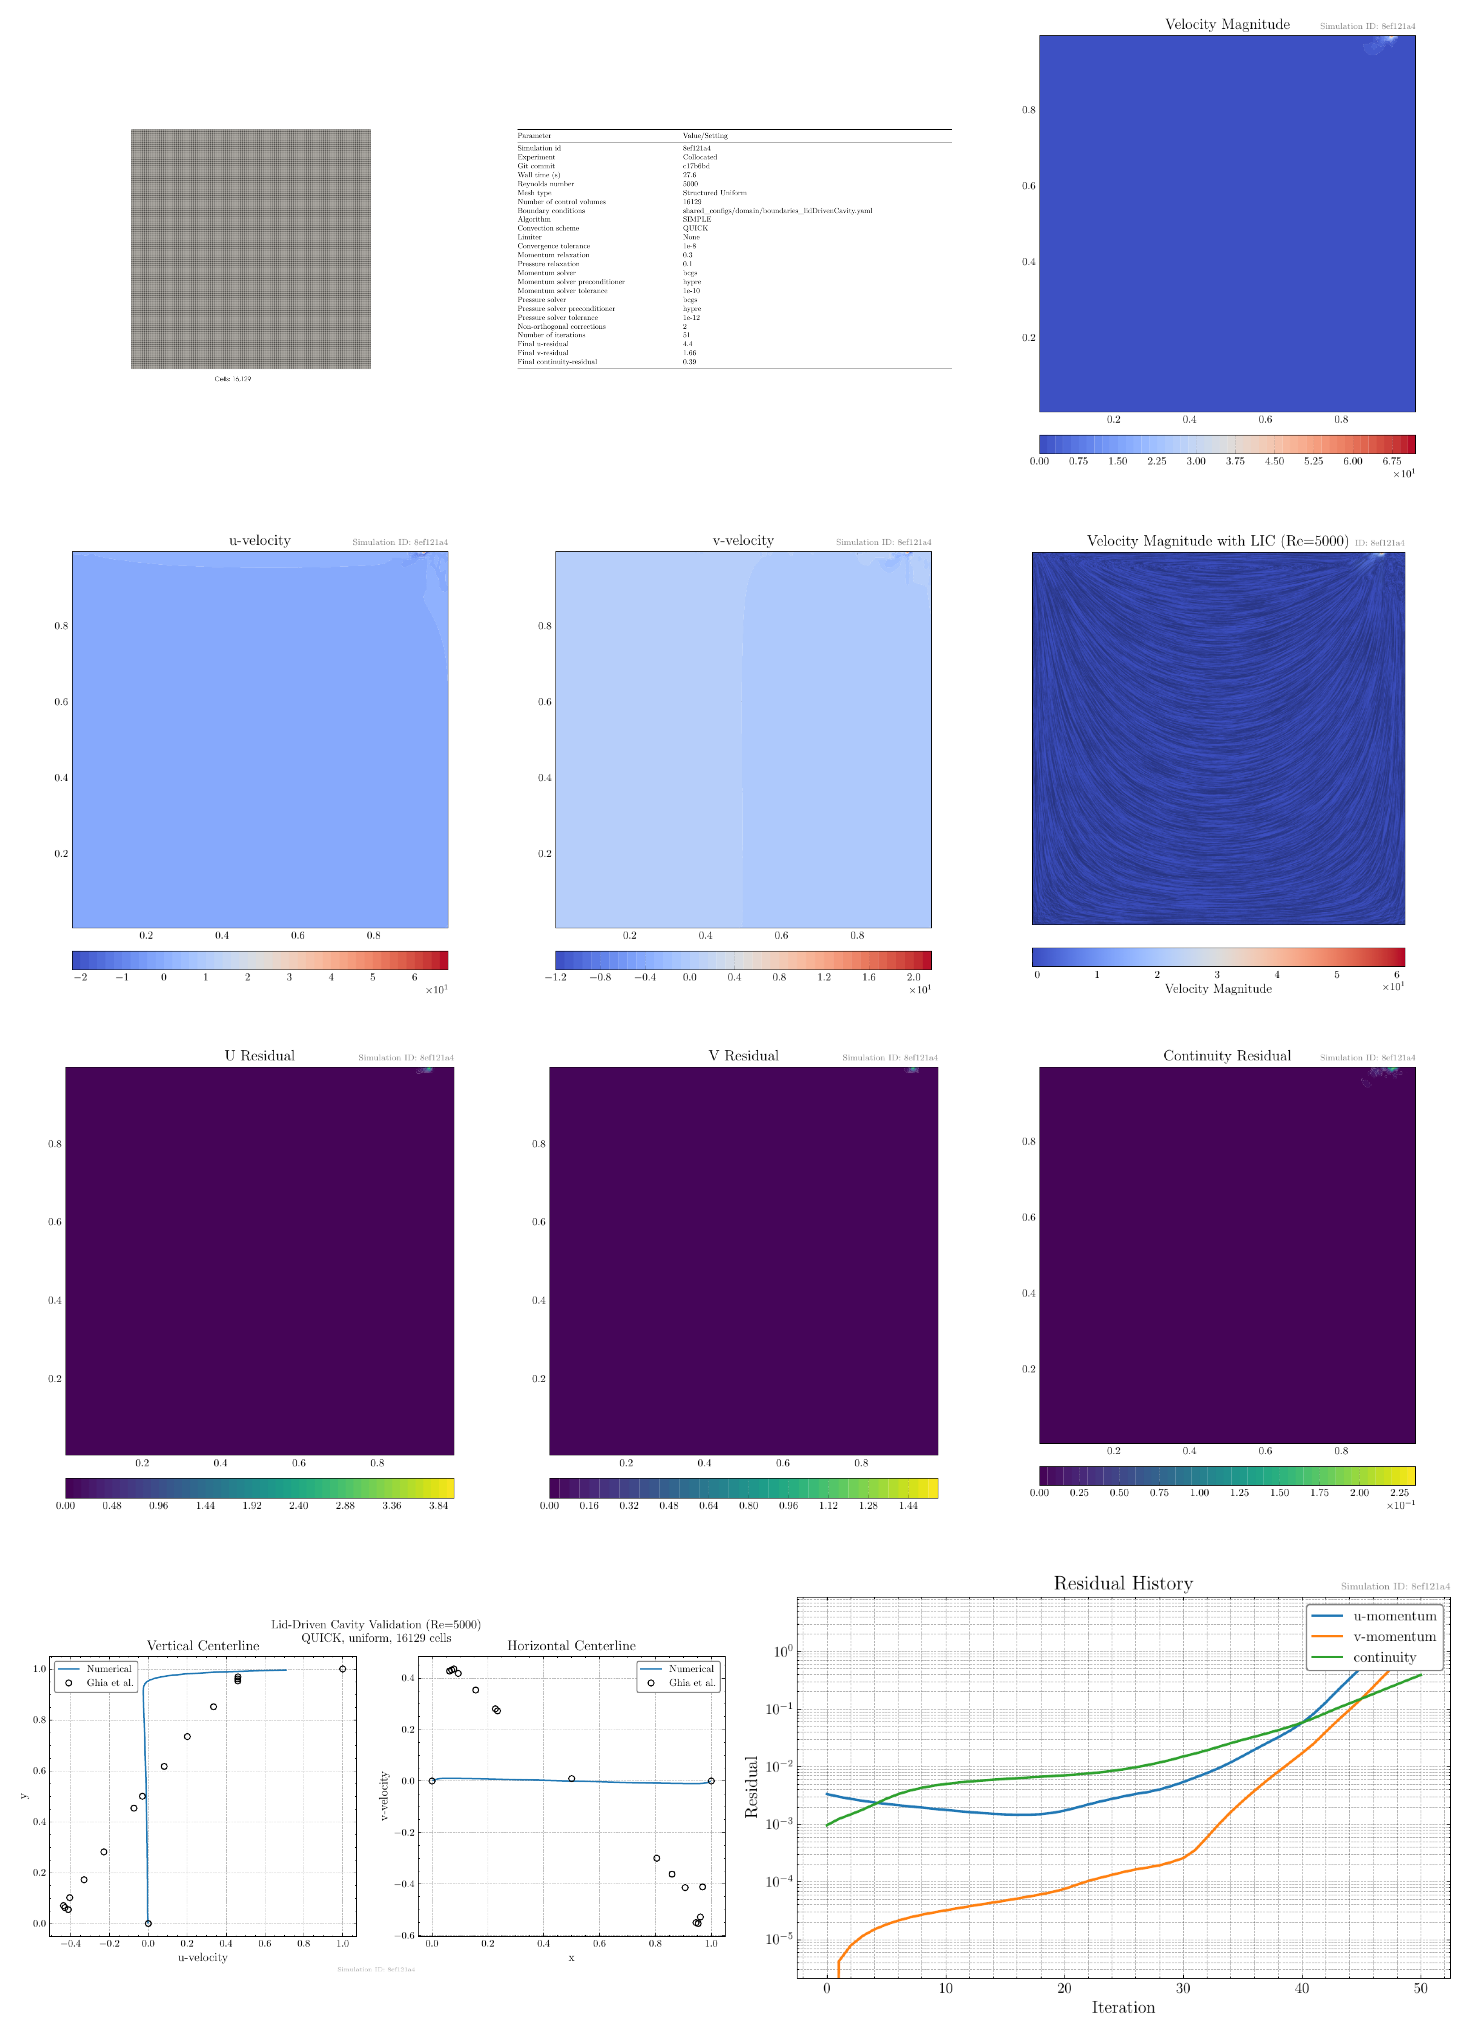
\includegraphics[width=0.85\linewidth]{AppendixPlots/lidDrivenCavity/Re_5000/medium/lidDrivenCavity_Re5000_uniform_medium_QUICK_8ef121a4.pdf}
    \caption{Liddrivencavity simulation at Re=5000 using uniform medium mesh with QUICK discretization scheme (Simulation ID: 8ef121a4)}
    \label{sim.ldc.re5000.unif.med.quick}
\end{figure}

\paragraph*{Uniform Mesh with TVD Scheme}
\addcontentsline{toc}{paragraph}{Uniform Mesh with TVD Scheme}
\label{para:liddrivencavity_re5000_medium_uniform_TVD}

\begin{figure}[H]
    \centering
    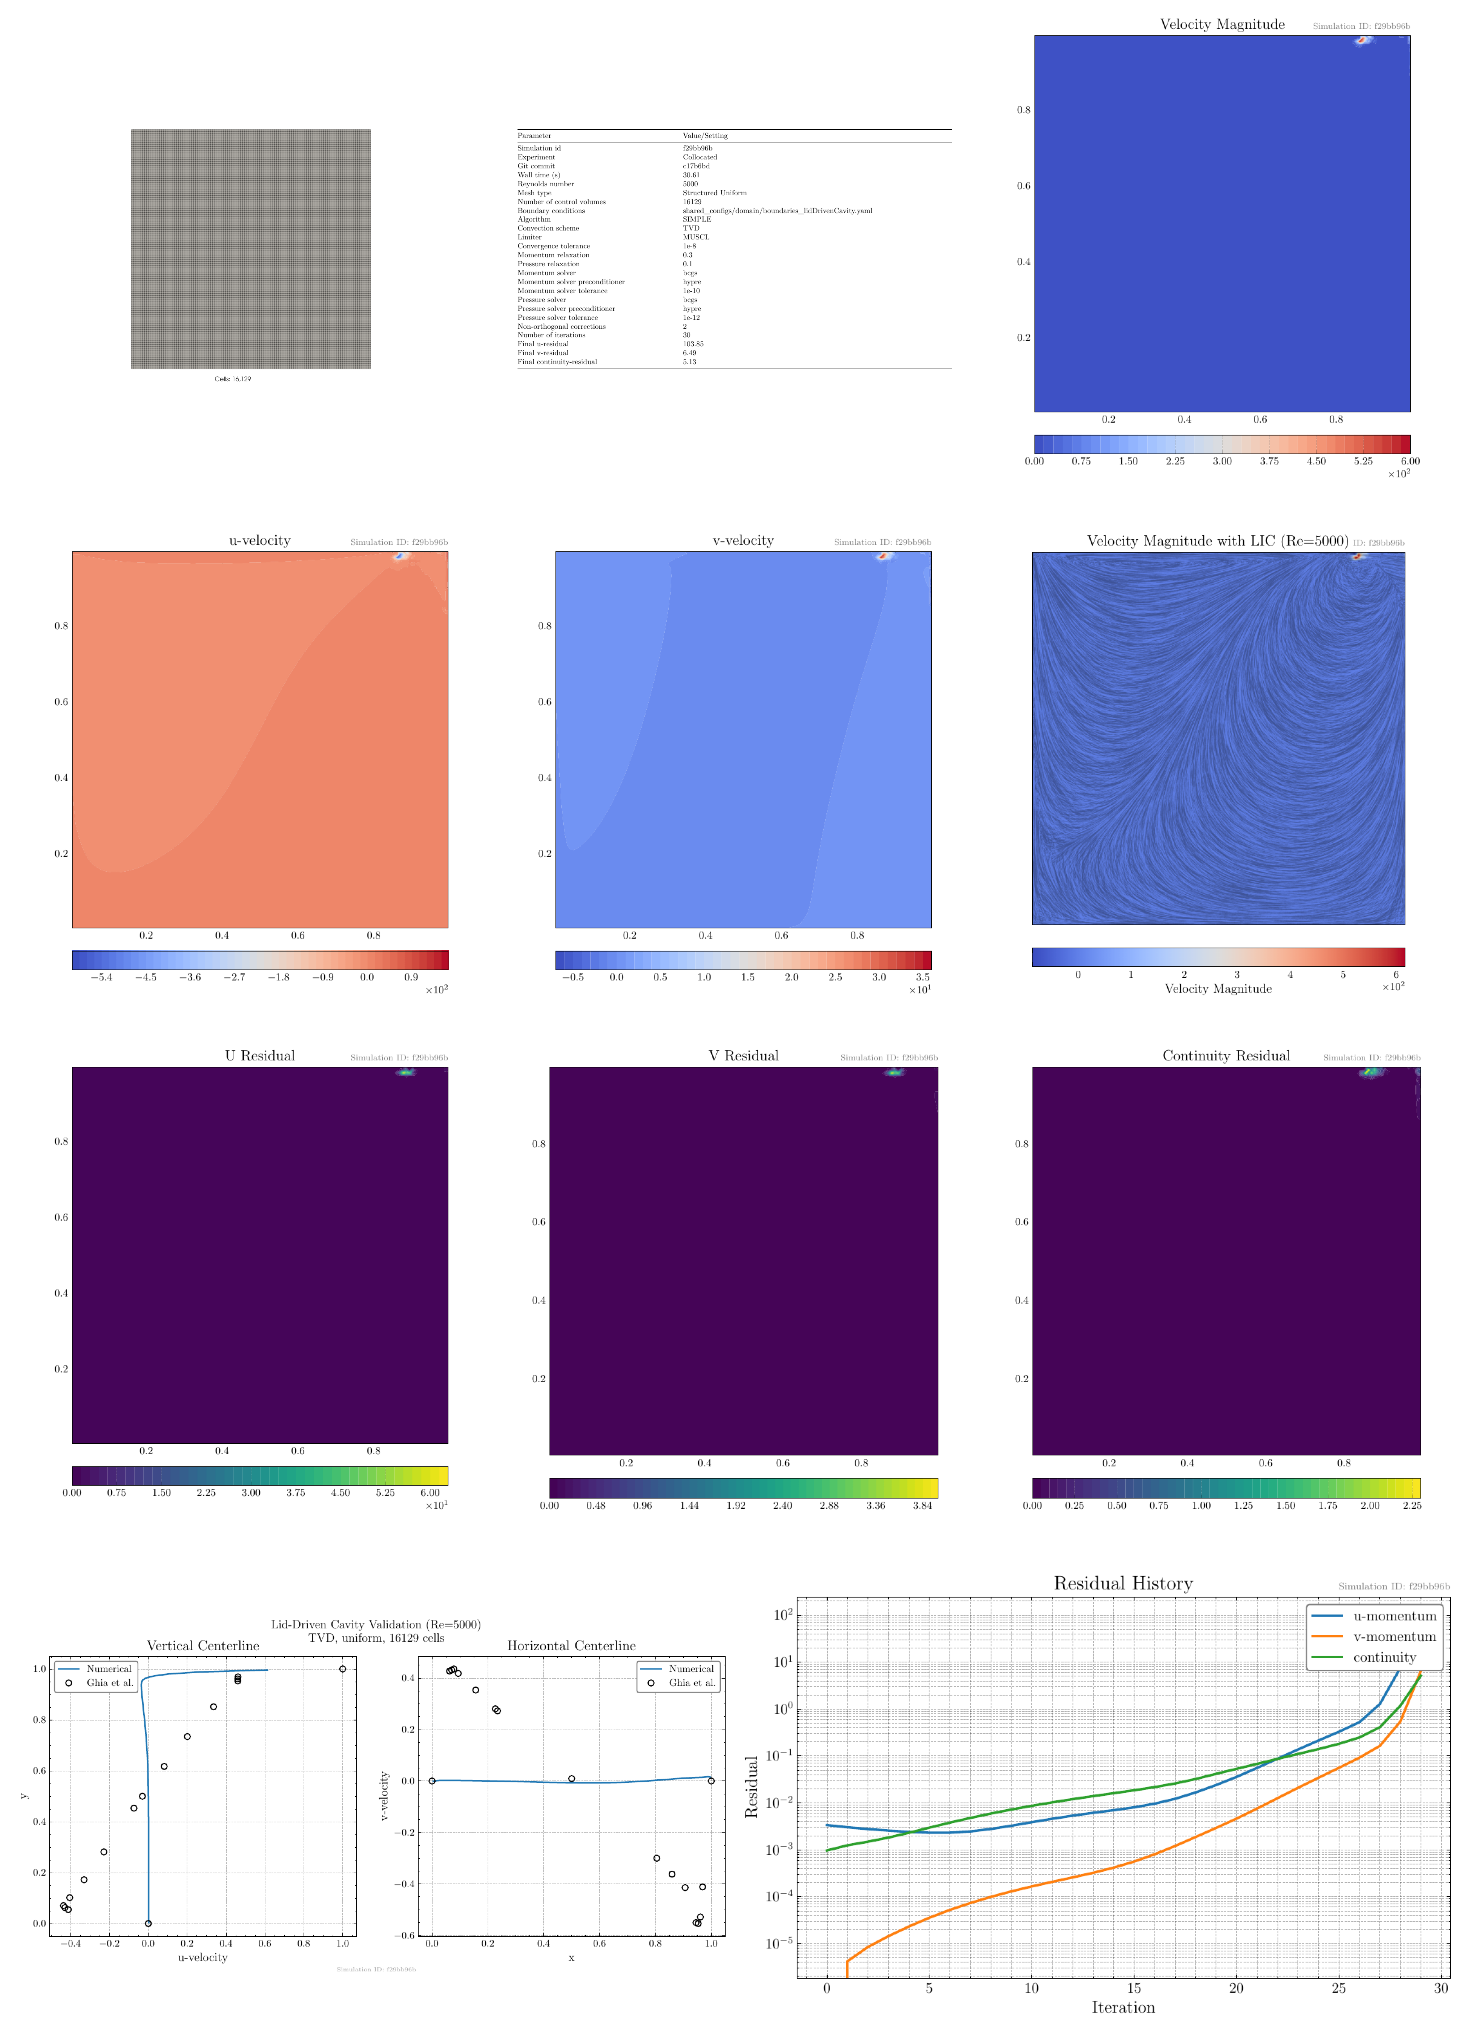
\includegraphics[width=0.85\linewidth]{AppendixPlots/lidDrivenCavity/Re_5000/medium/lidDrivenCavity_Re5000_uniform_medium_TVD_f29bb96b.pdf}
    \caption{Liddrivencavity simulation at Re=5000 using uniform medium mesh with TVD discretization scheme (Simulation ID: f29bb96b)}
    \label{sim.ldc.re5000.unif.med.tvd}
\end{figure}

\paragraph*{Uniform Mesh with Upwind Scheme}
\addcontentsline{toc}{paragraph}{Uniform Mesh with Upwind Scheme}
\label{para:liddrivencavity_re5000_medium_uniform_Upwind}

\begin{figure}[H]
    \centering
    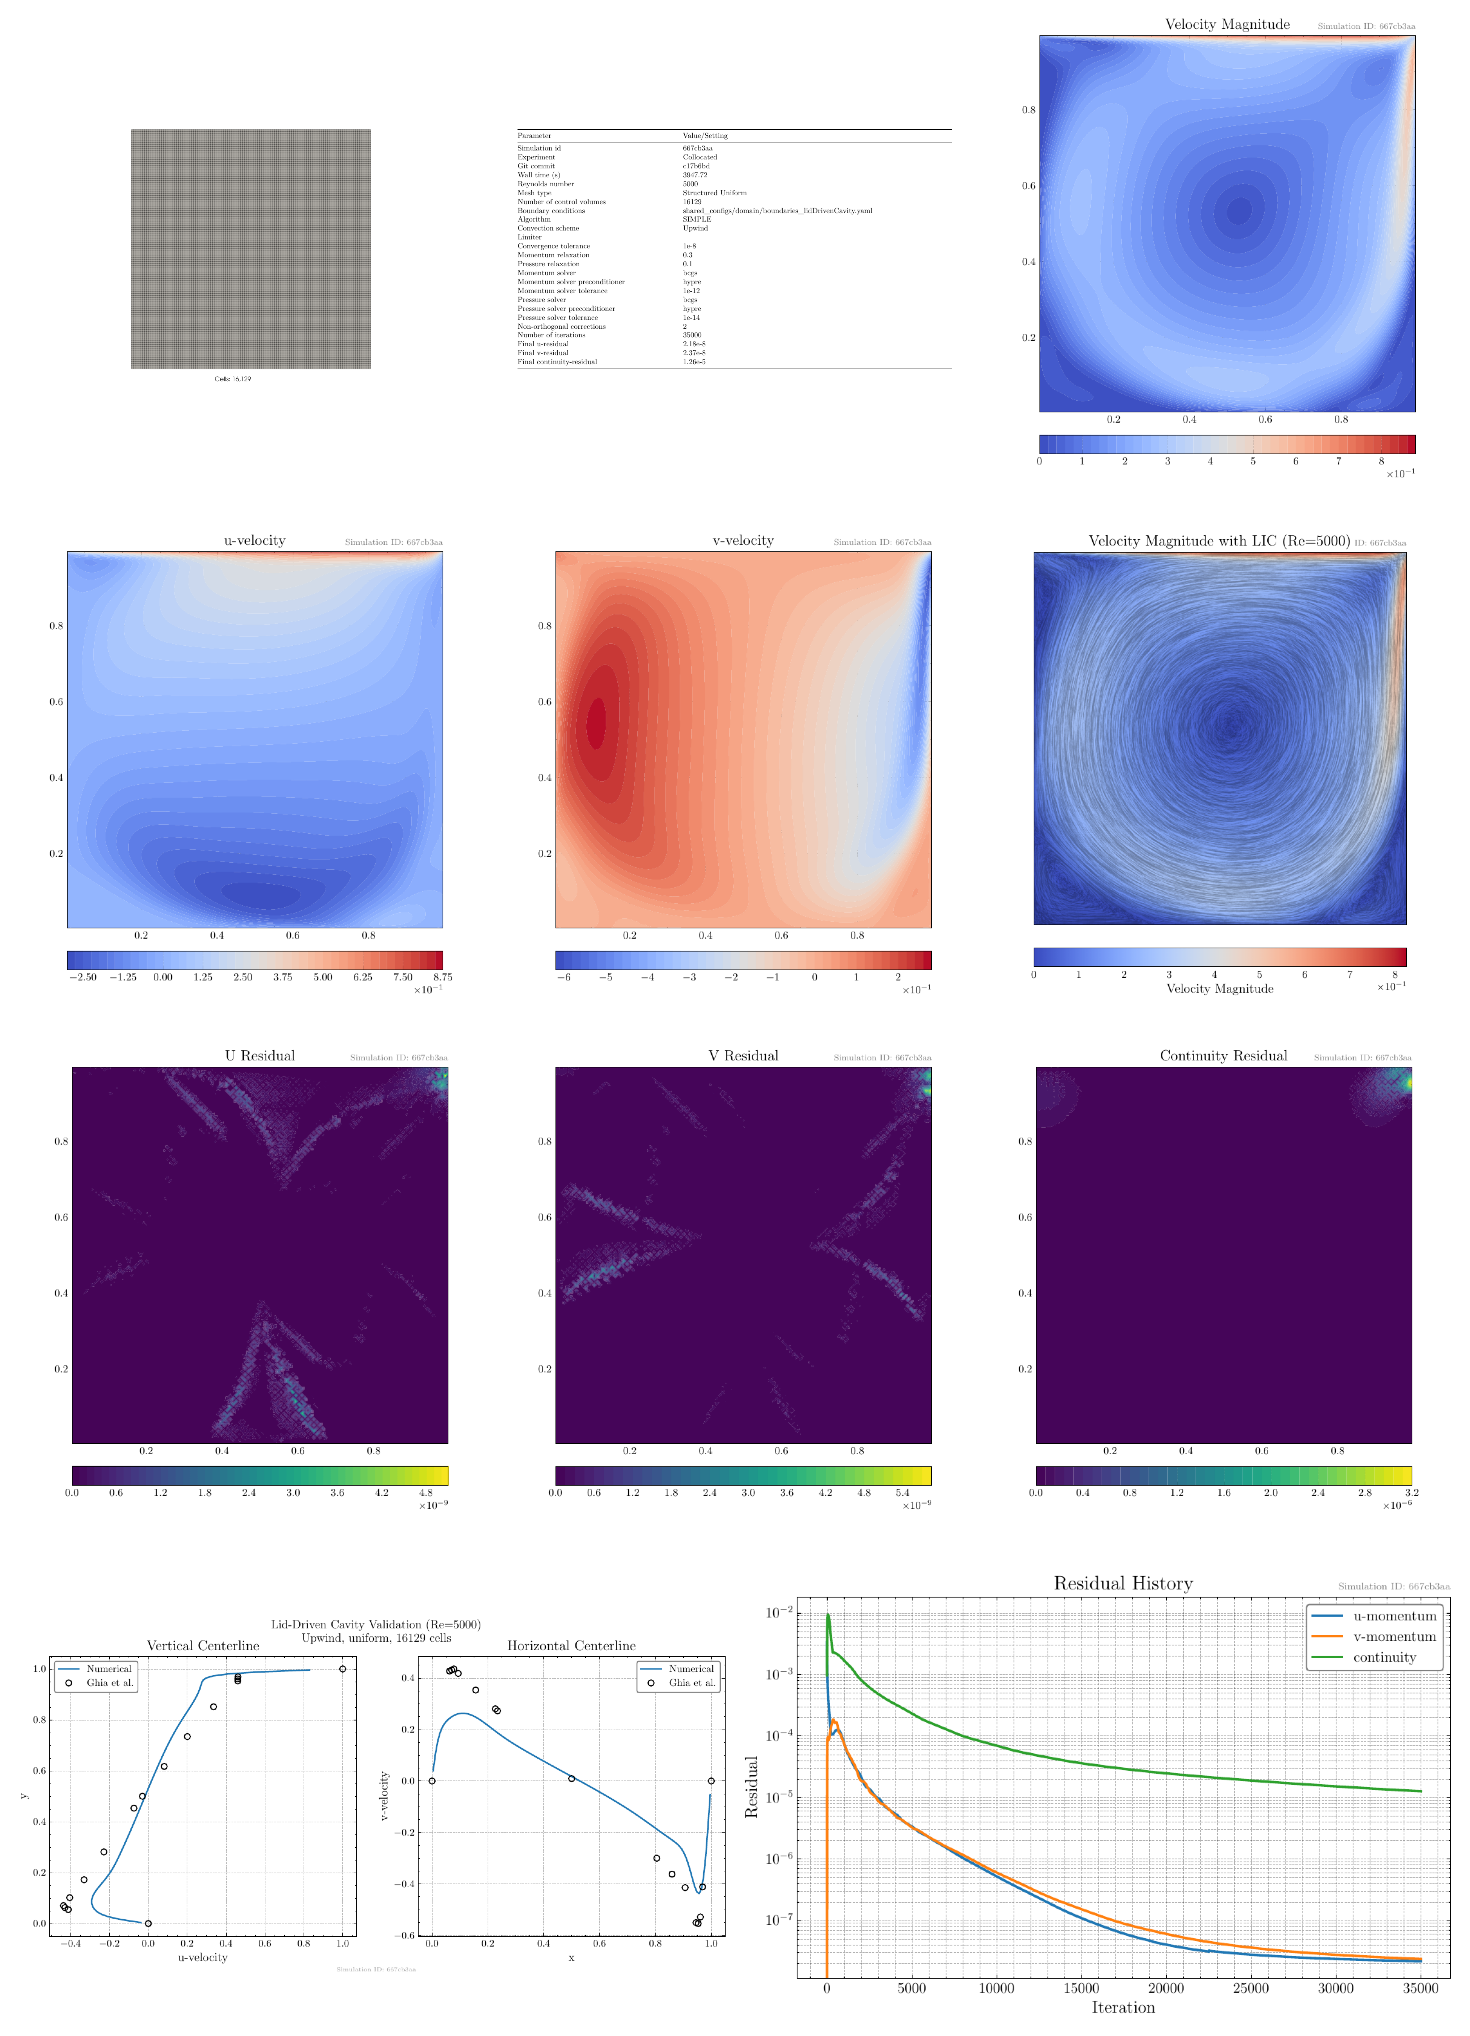
\includegraphics[width=0.85\linewidth]{AppendixPlots/lidDrivenCavity/Re_5000/medium/lidDrivenCavity_Re5000_uniform_medium_Upwind_667cb3aa.pdf}
    \caption{Liddrivencavity simulation at Re=5000 using uniform medium mesh with Upwind discretization scheme (Simulation ID: 667cb3aa)}
    \label{sim.ldc.re5000.unif.med.upwind}
\end{figure}

\paragraph*{Unstructured Mesh with QUICK Scheme}
\addcontentsline{toc}{paragraph}{Unstructured Mesh with QUICK Scheme}
\label{para:liddrivencavity_re5000_medium_unstructured_QUICK}

\begin{figure}[H]
    \centering
    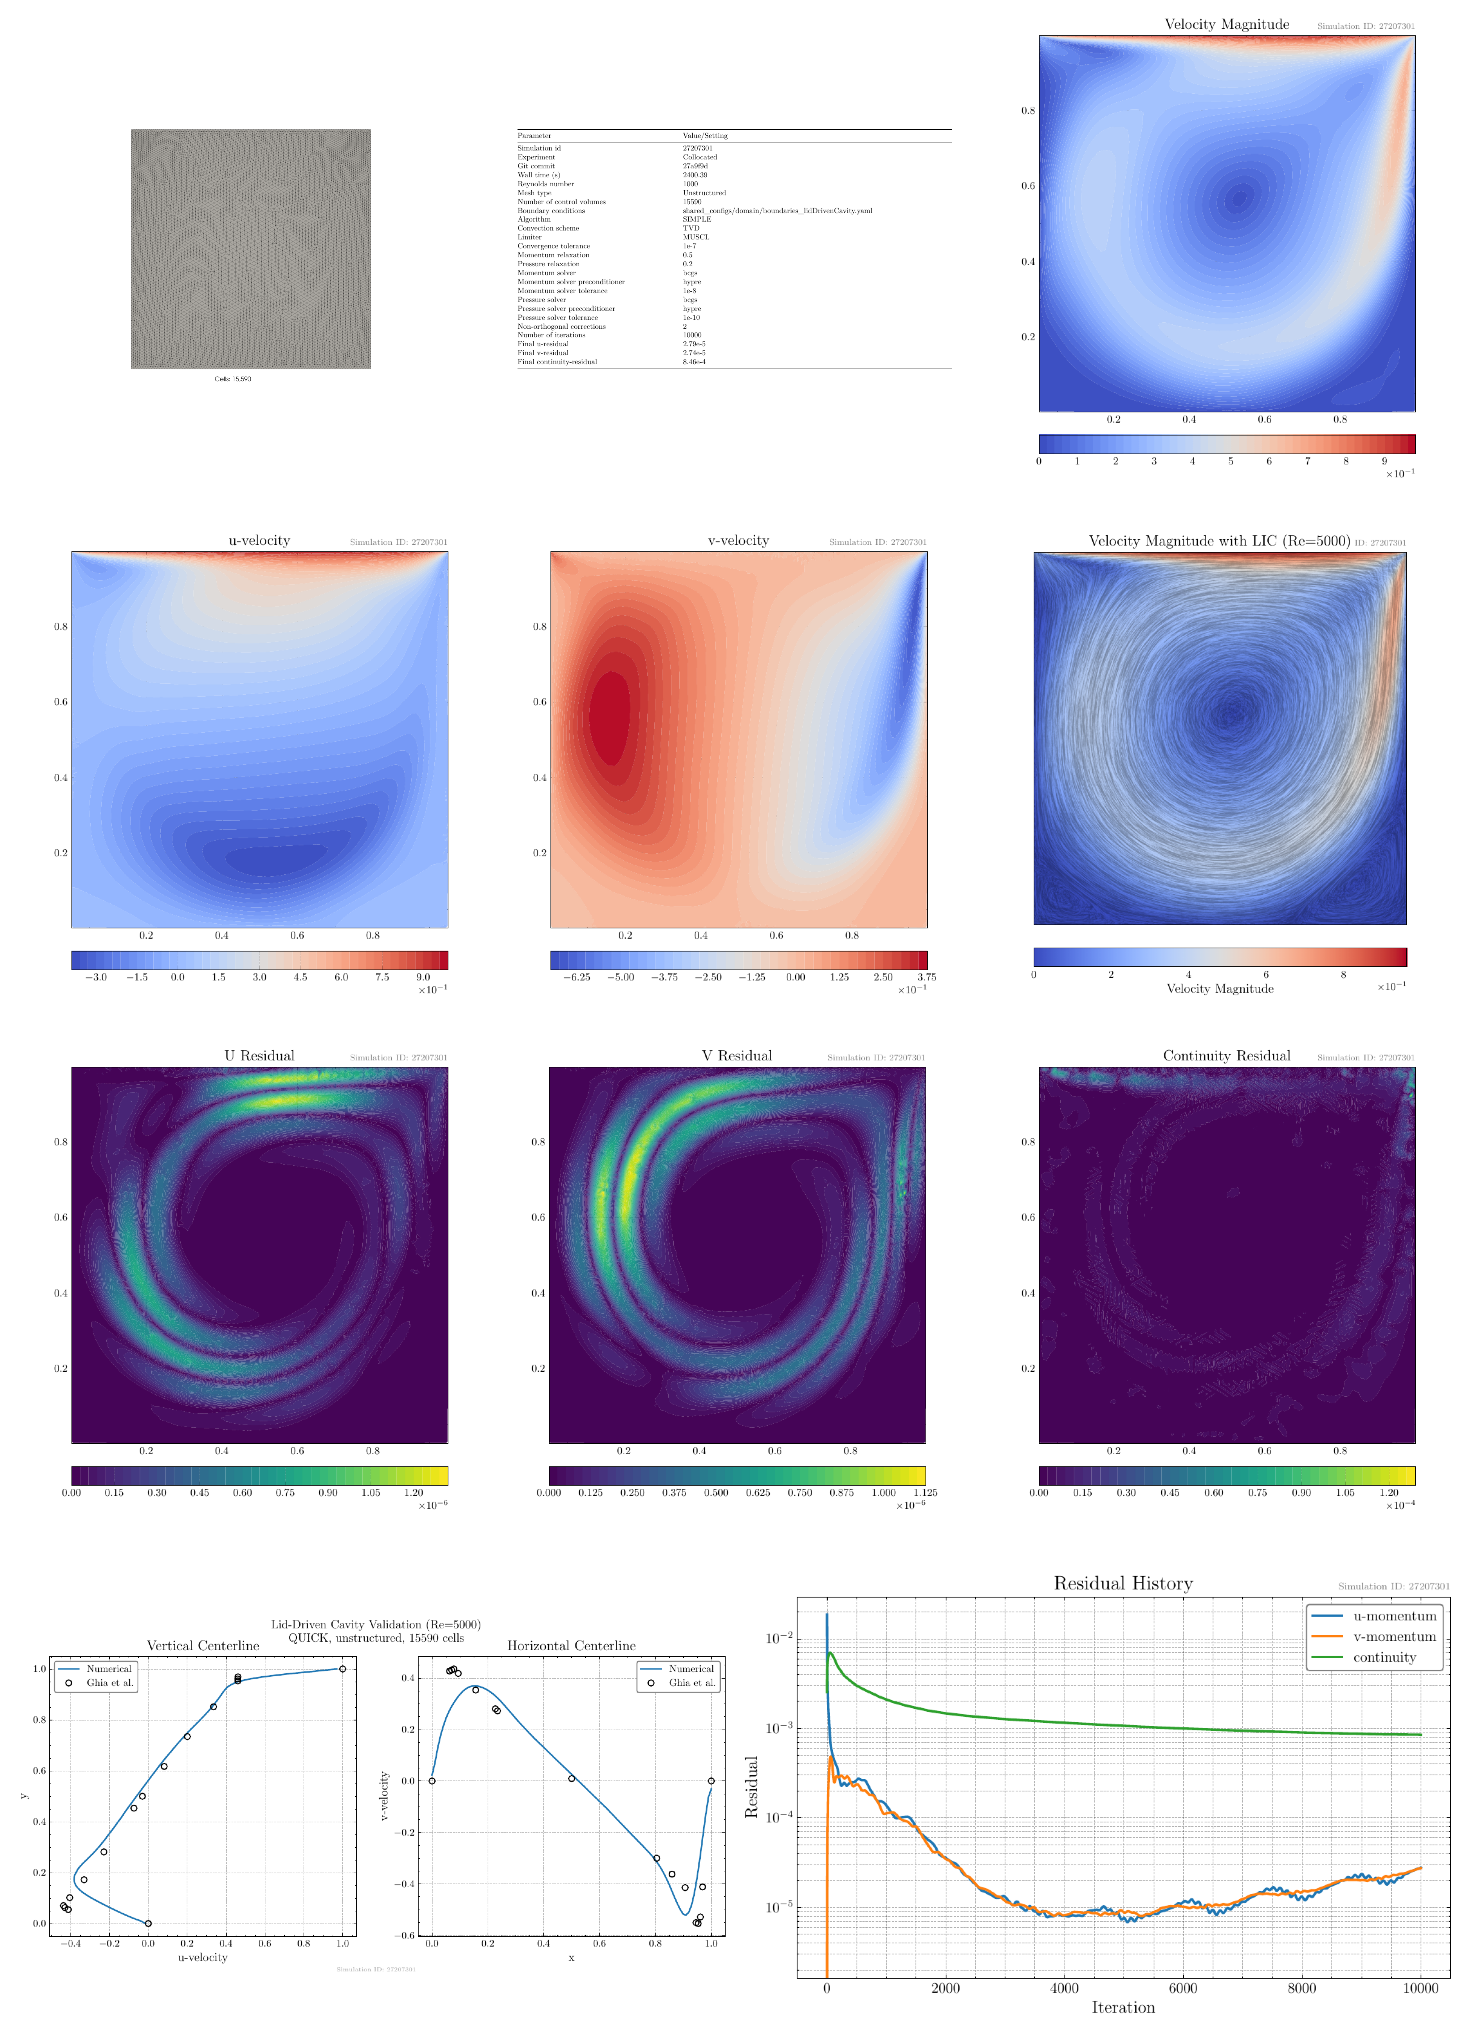
\includegraphics[width=0.85\linewidth]{AppendixPlots/lidDrivenCavity/Re_5000/medium/lidDrivenCavity_Re5000_unstructured_medium_QUICK_27207301.pdf}
    \caption{Liddrivencavity simulation at Re=5000 using unstructured medium mesh with QUICK discretization scheme (Simulation ID: 27207301)}
    \label{sim.ldc.re5000.unstruct.med.quick}
\end{figure}

\paragraph*{Unstructured Mesh with TVD Scheme}
\addcontentsline{toc}{paragraph}{Unstructured Mesh with TVD Scheme}
\label{para:liddrivencavity_re5000_medium_unstructured_TVD}

\begin{figure}[H]
    \centering
    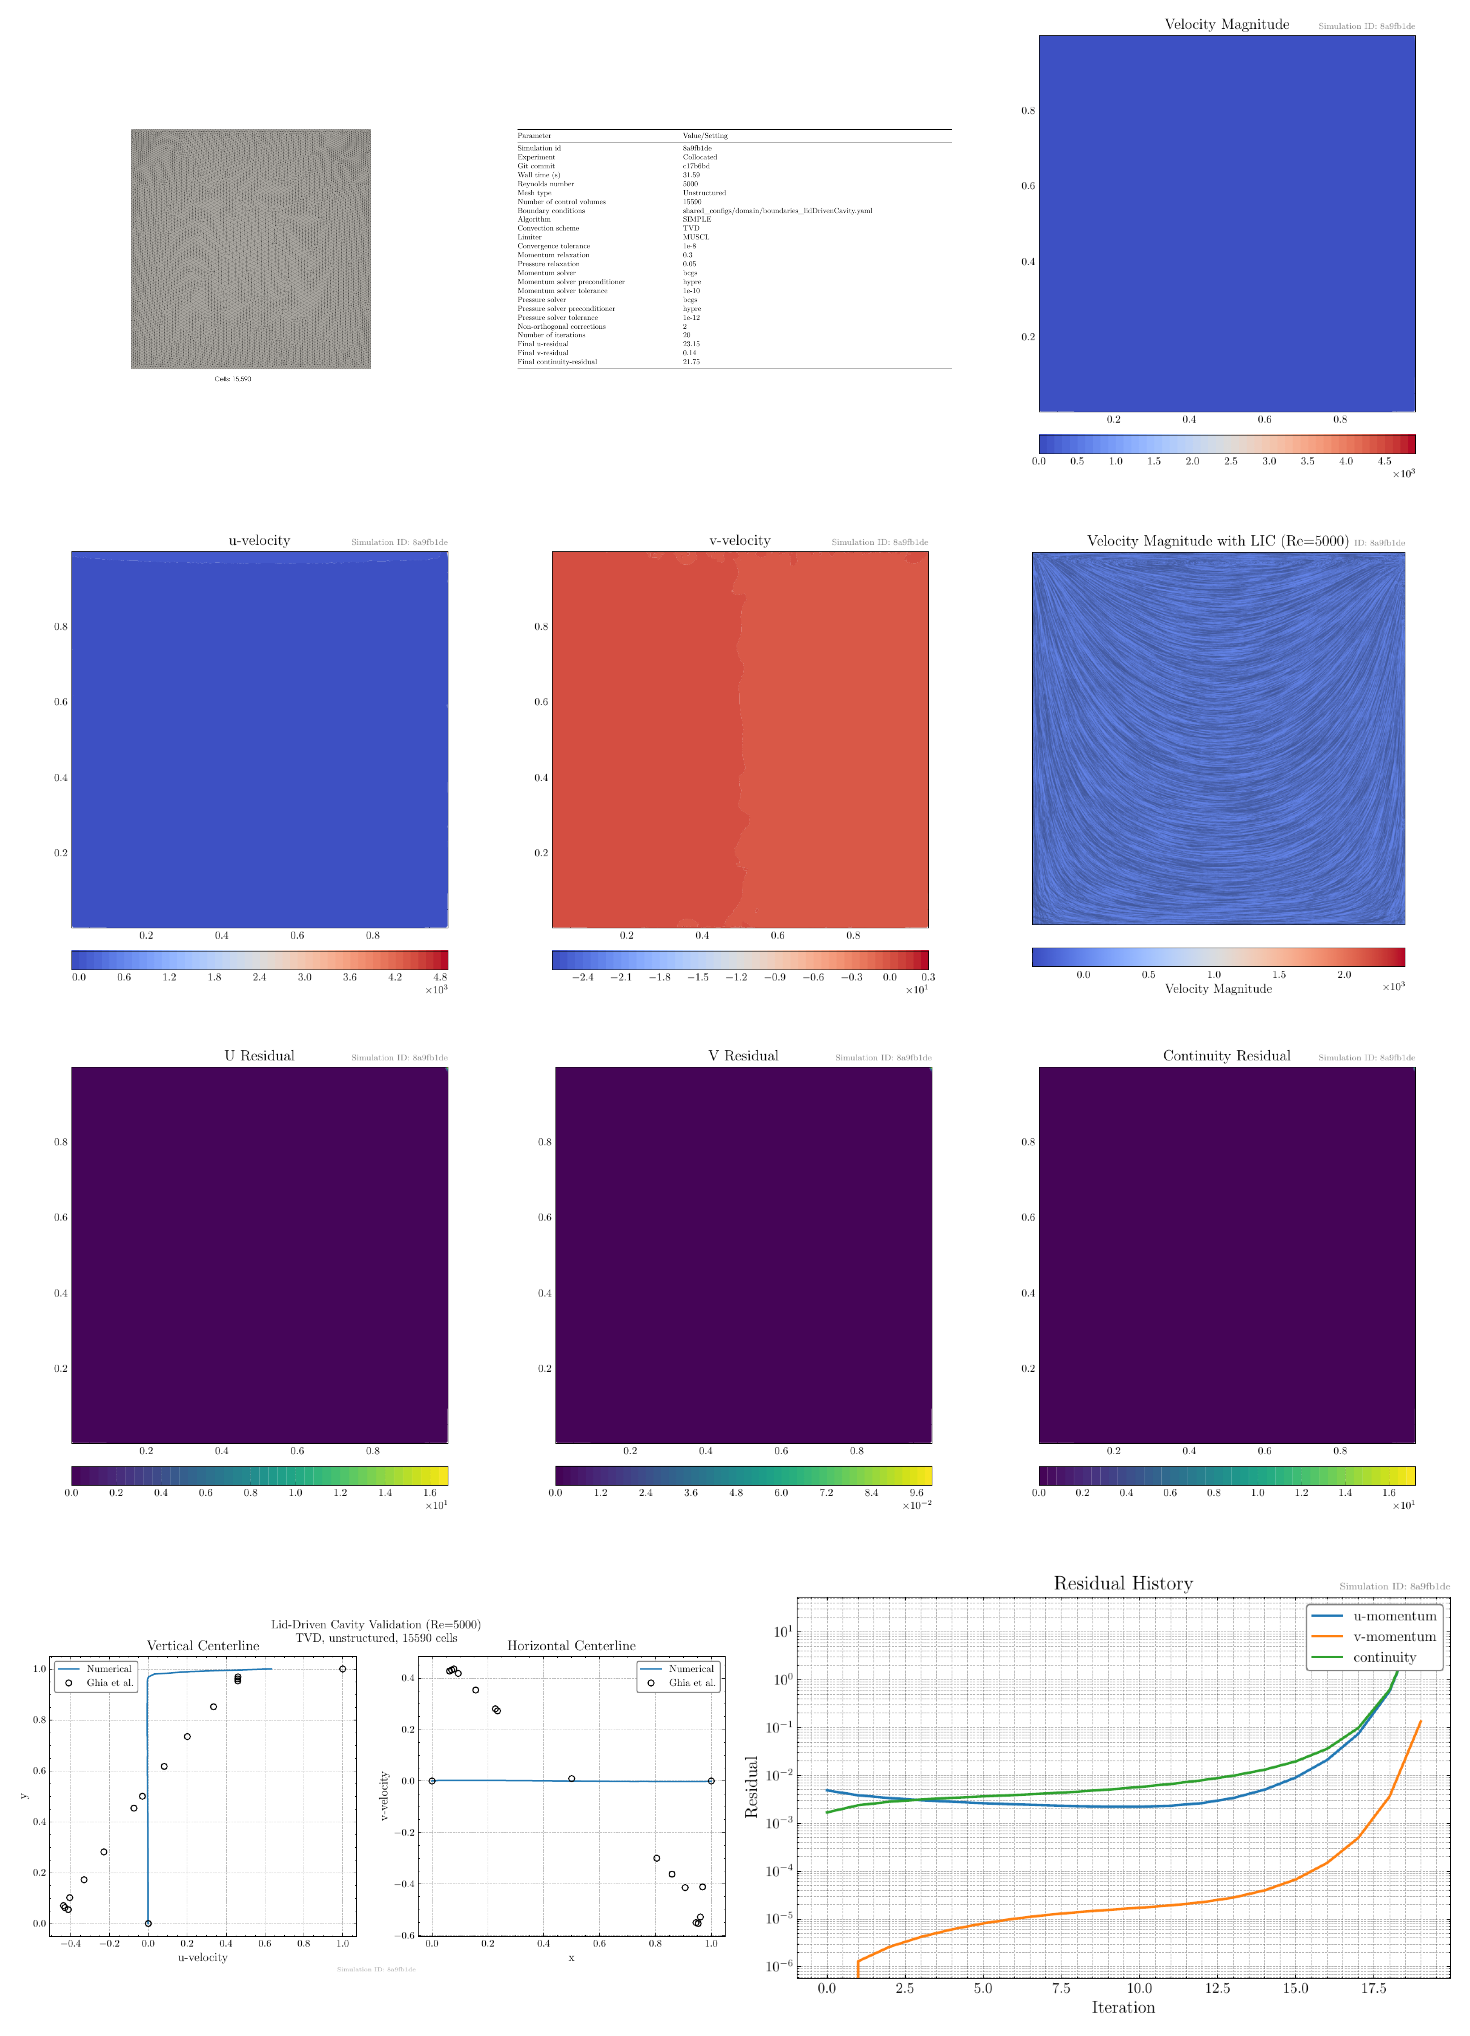
\includegraphics[width=0.85\linewidth]{AppendixPlots/lidDrivenCavity/Re_5000/medium/lidDrivenCavity_Re5000_unstructured_medium_TVD_8a9fb1de.pdf}
    \caption{Liddrivencavity simulation at Re=5000 using unstructured medium mesh with TVD discretization scheme (Simulation ID: 8a9fb1de)}
    \label{sim.ldc.re5000.unstruct.med.tvd}
\end{figure}

\paragraph*{Unstructured Mesh with Upwind Scheme}
\addcontentsline{toc}{paragraph}{Unstructured Mesh with Upwind Scheme}
\label{para:liddrivencavity_re5000_medium_unstructured_Upwind}

\begin{figure}[H]
    \centering
    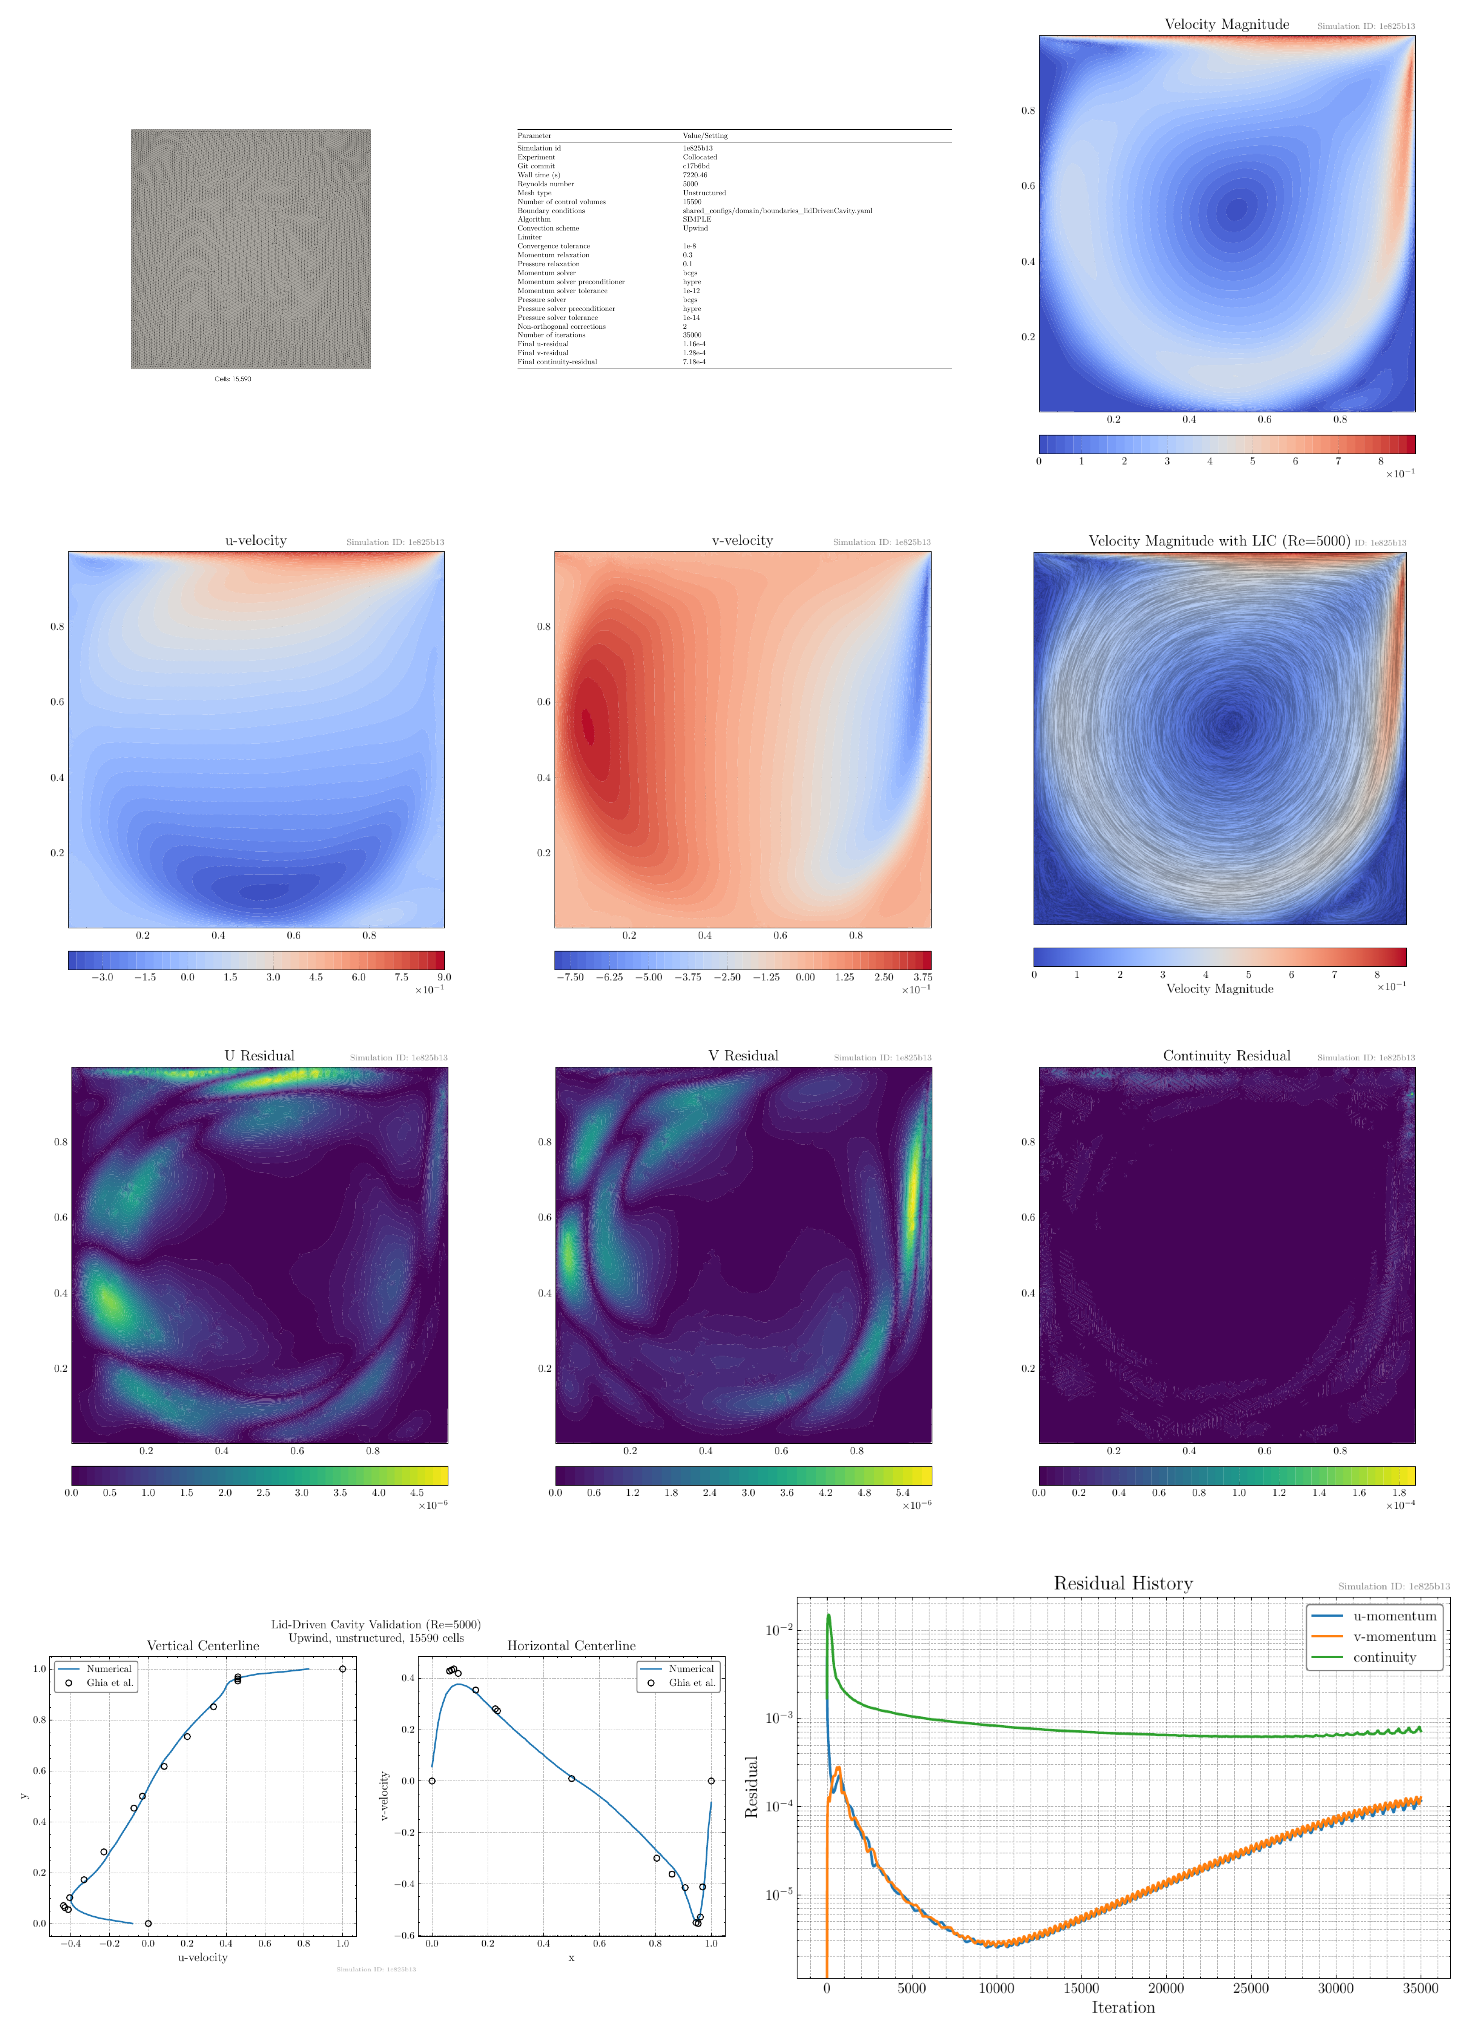
\includegraphics[width=0.85\linewidth]{AppendixPlots/lidDrivenCavity/Re_5000/medium/lidDrivenCavity_Re5000_unstructured_medium_Upwind_1e825b13.pdf}
    \caption{Liddrivencavity simulation at Re=5000 using unstructured medium mesh with Upwind discretization scheme (Simulation ID: 1e825b13)}
    \label{sim.ldc.re5000.unstruct.med.upwind}
\end{figure}

\clearpage

\subsubsection*{Fine Mesh}
\addcontentsline{toc}{subsubsection}{Fine Mesh}
\label{subsubsec:liddrivencavity_re5000_fine}

\paragraph*{Uniform Mesh with Upwind Scheme}
\addcontentsline{toc}{paragraph}{Uniform Mesh with Upwind Scheme}
\label{para:liddrivencavity_re5000_fine_uniform_Upwind}

\begin{figure}[H]
    \centering
    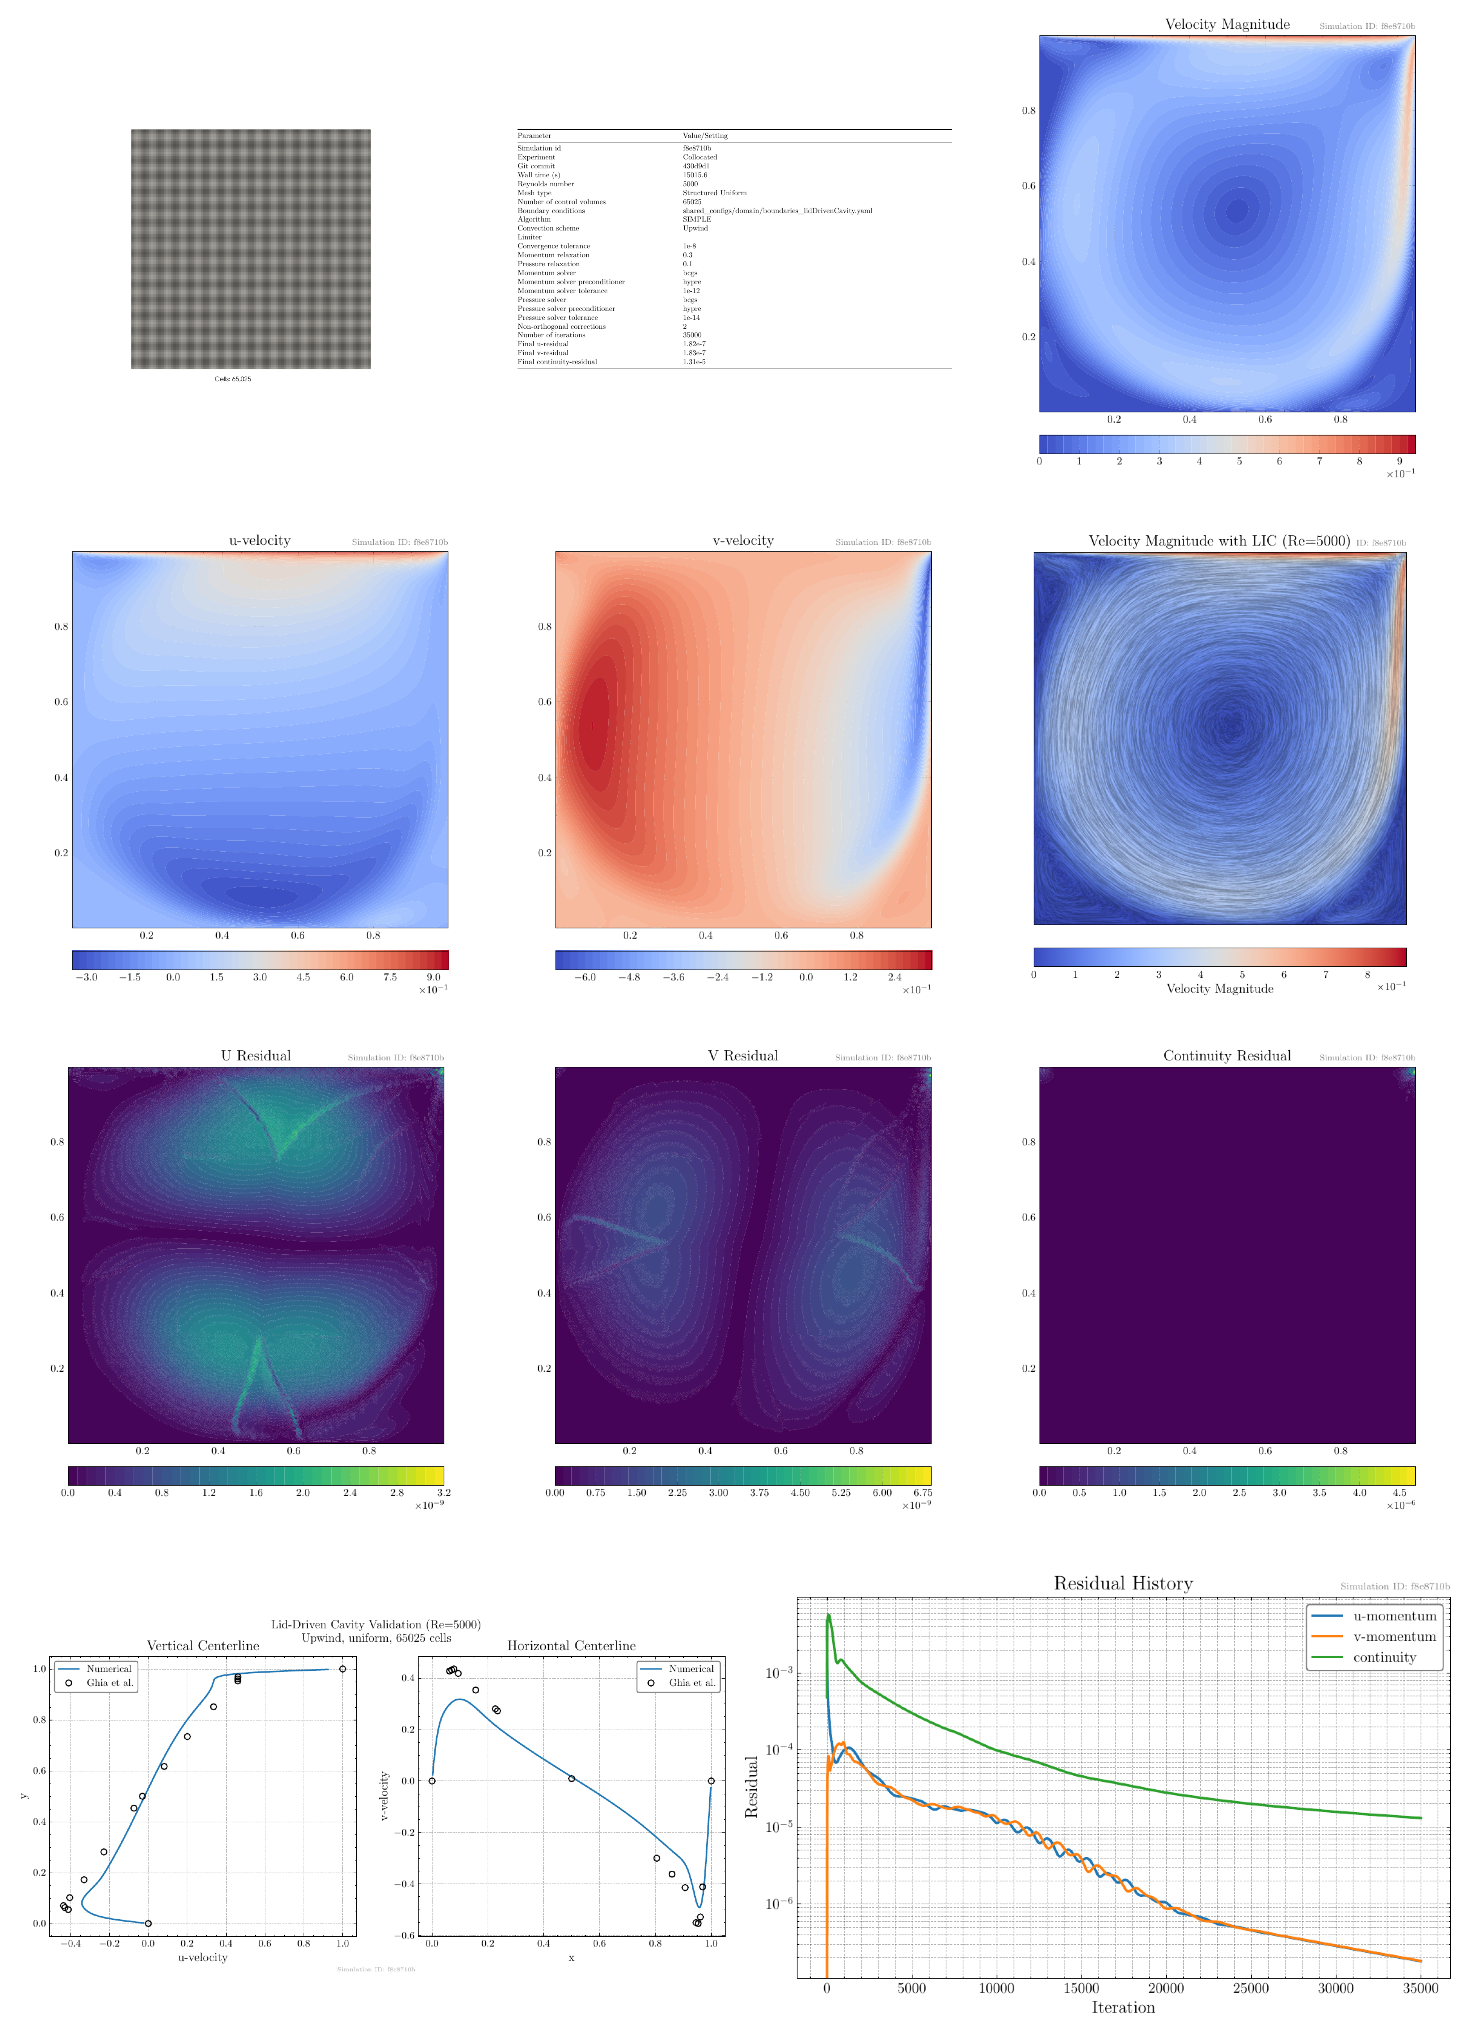
\includegraphics[width=0.85\linewidth]{AppendixPlots/lidDrivenCavity/Re_5000/fine/lidDrivenCavity_Re5000_uniform_fine_Upwind_f8e8710b.pdf}
    \caption{Liddrivencavity simulation at Re=5000 using uniform fine mesh with Upwind discretization scheme (Simulation ID: f8e8710b)}
    \label{sim.ldc.re5000.unif.fine.upwind}
\end{figure}

\paragraph*{Unstructured Mesh with Upwind Scheme}
\addcontentsline{toc}{paragraph}{Unstructured Mesh with Upwind Scheme}
\label{para:liddrivencavity_re5000_fine_unstructured_Upwind}

\begin{figure}[H]
    \centering
    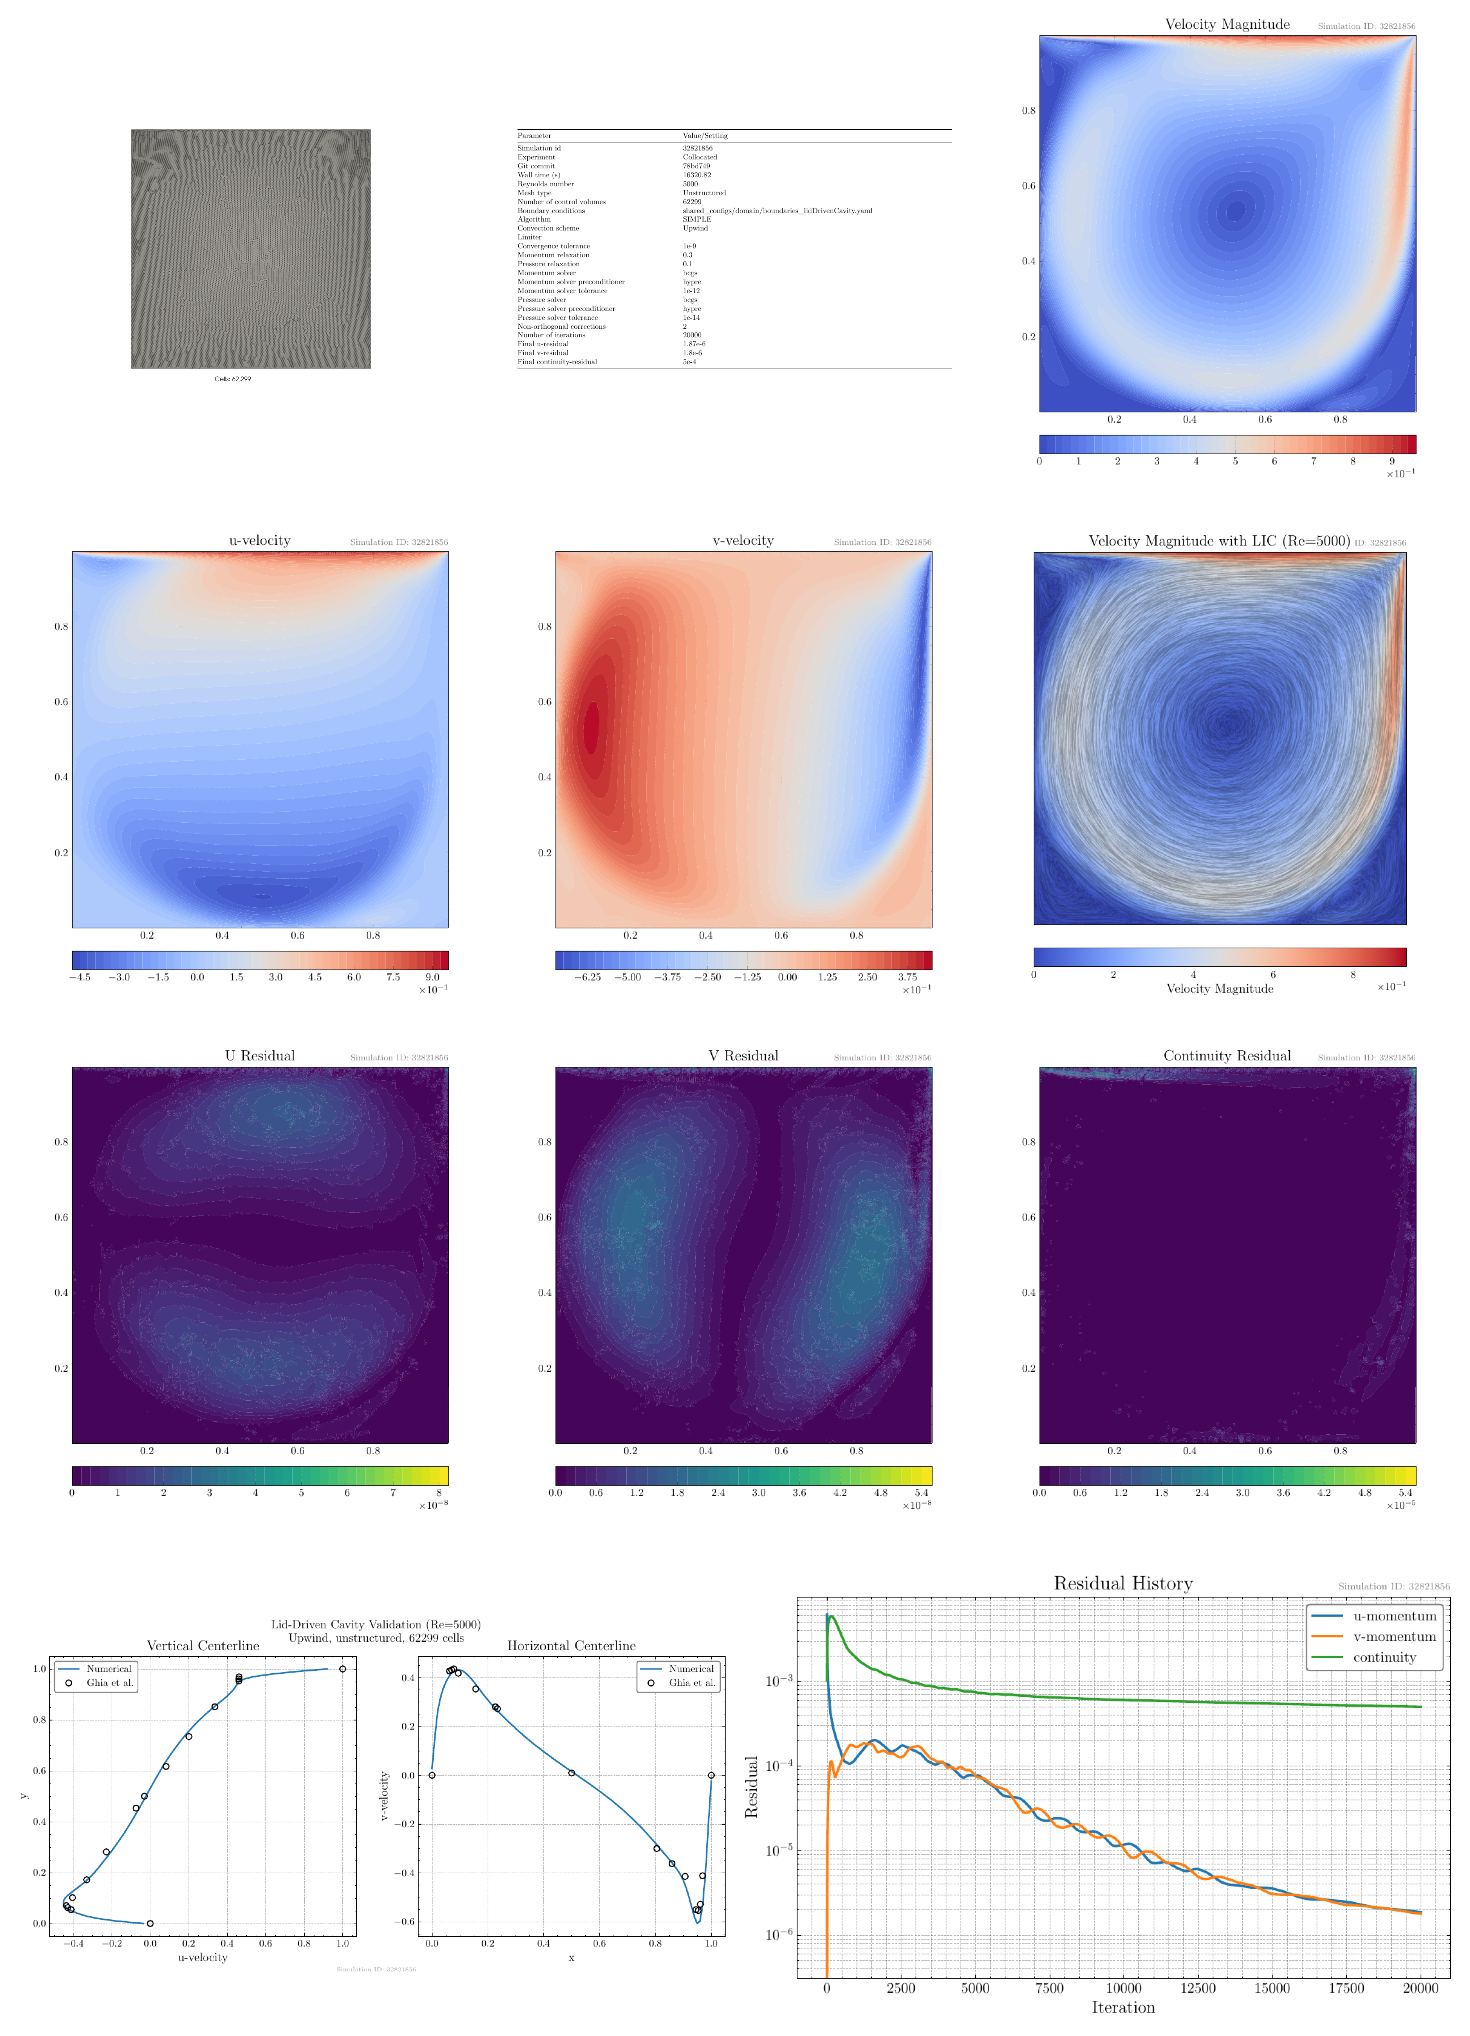
\includegraphics[width=0.85\linewidth]{AppendixPlots/lidDrivenCavity/Re_5000/fine/lidDrivenCavity_Re5000_unstructured_fine_Upwind_32821856.pdf}
    \caption{Liddrivencavity simulation at Re=5000 using unstructured fine mesh with Upwind discretization scheme (Simulation ID: 32821856)}
    \label{sim.ldc.re5000.unstruct.fine.upwind}
\end{figure}

\clearpage

\subsubsection*{127X127 Mesh}
\addcontentsline{toc}{subsubsection}{127X127 Mesh}
\label{subsubsec:liddrivencavity_re5000_127x127}

\paragraph*{Structured Mesh with Power Law Scheme}
\addcontentsline{toc}{paragraph}{Structured Mesh with Power Law Scheme}
\label{para:liddrivencavity_re5000_127x127_structured_Power Law}

\begin{figure}[H]
    \centering
    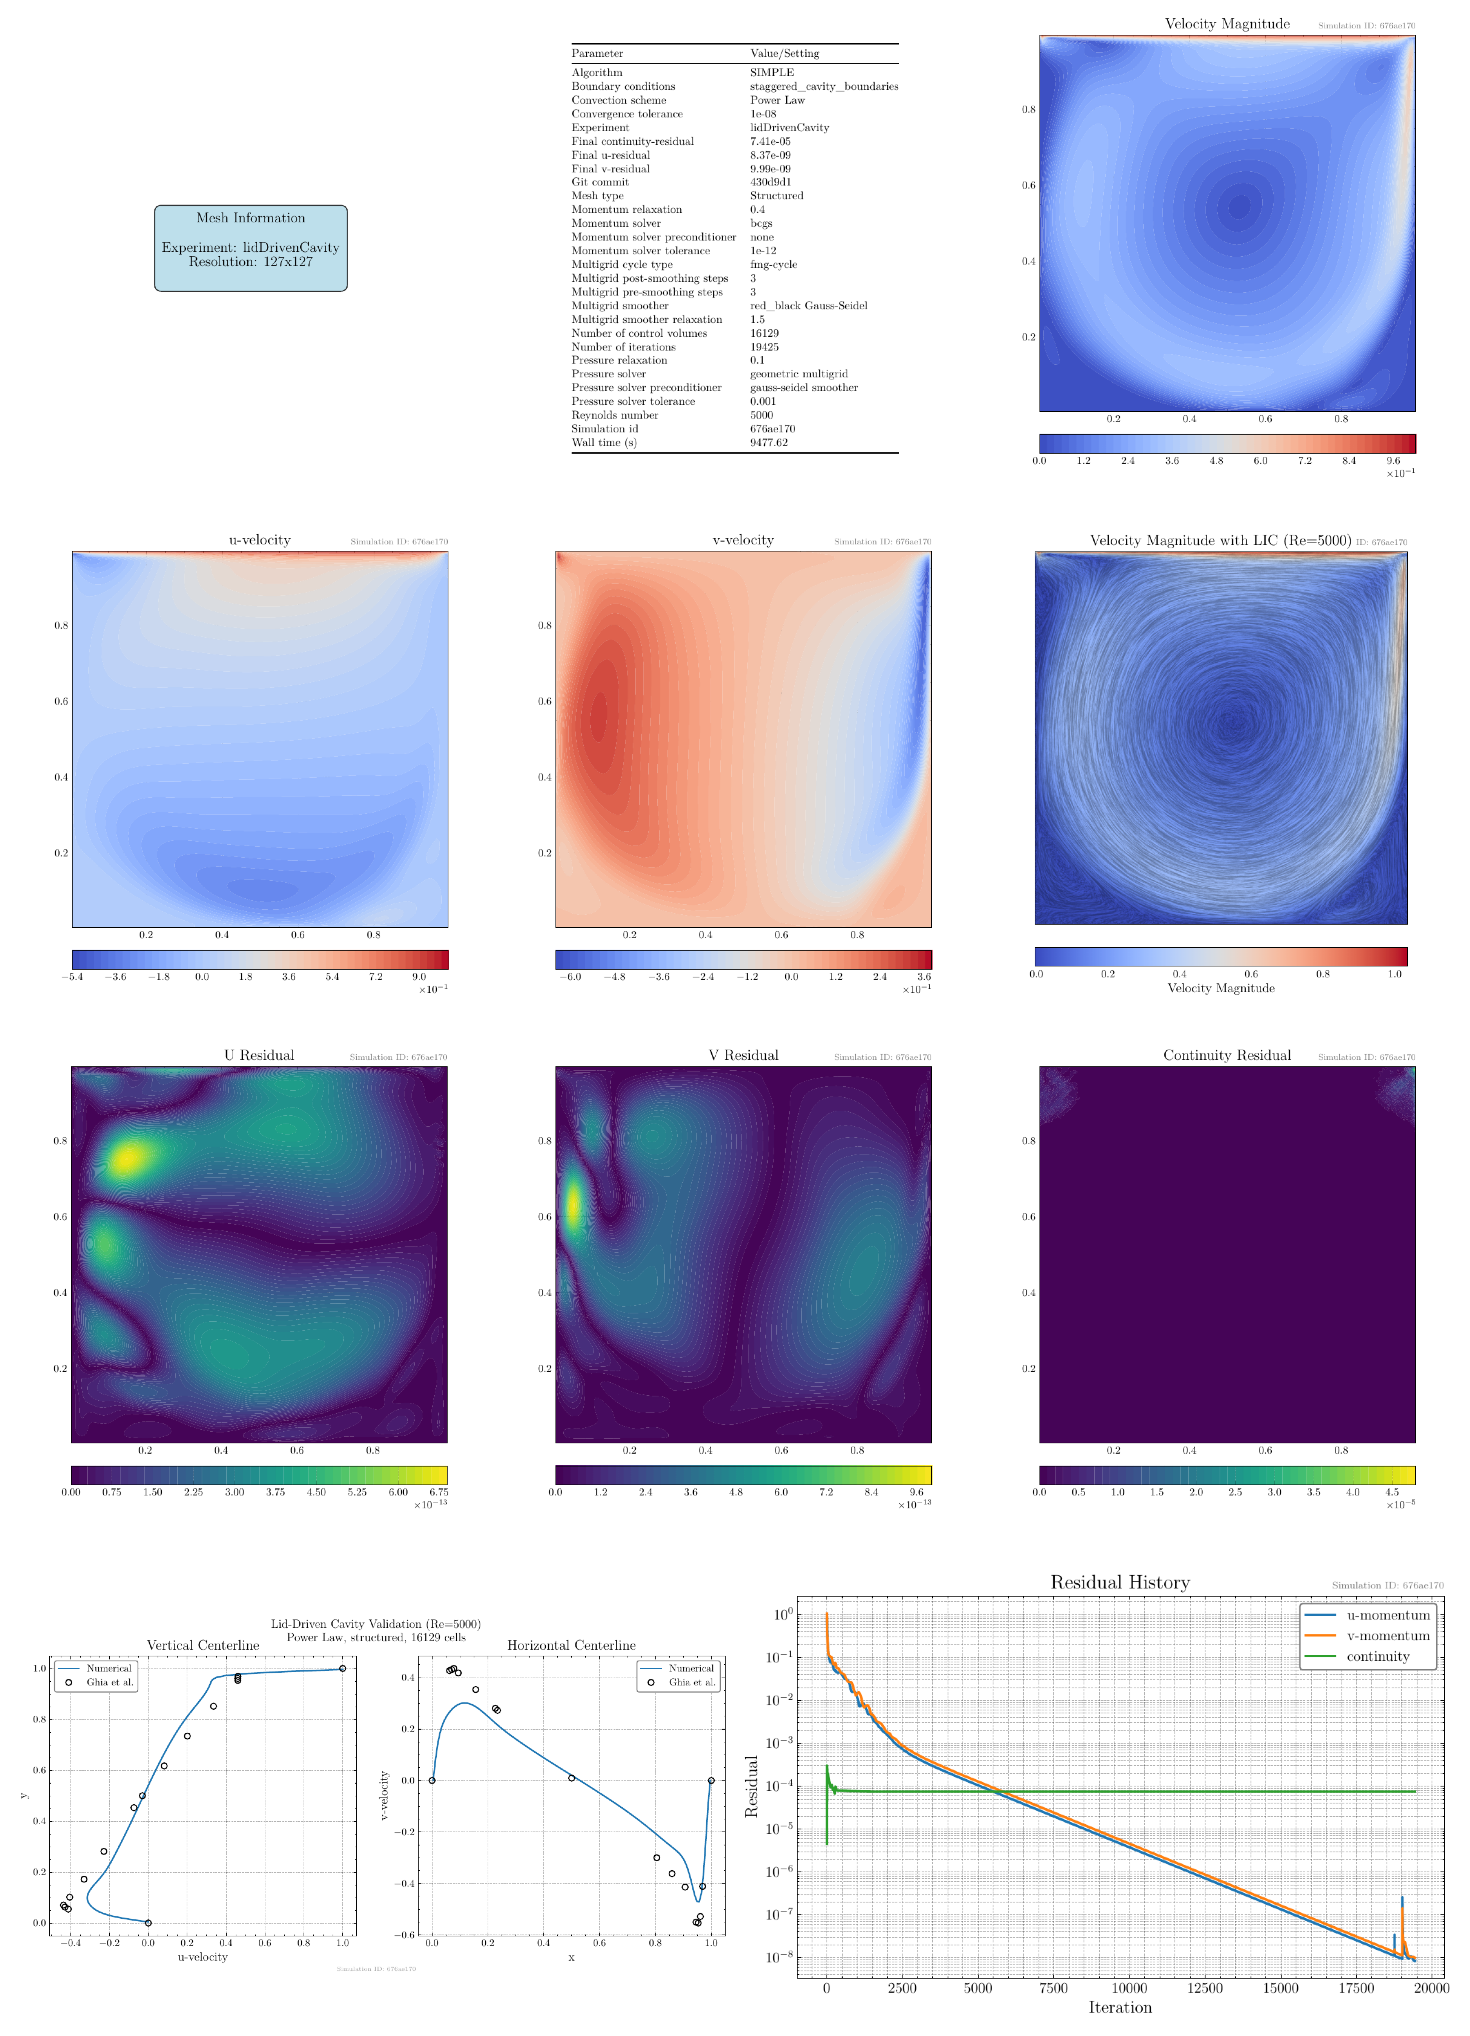
\includegraphics[width=0.85\linewidth]{AppendixPlots/lidDrivenCavity/Re_5000/127x127/lidDrivenCavity_Re5000_structured_127x127_Power Law_676ae170.pdf}
    \caption{Liddrivencavity simulation at Re=5000 using structured 127x127 (medium) mesh with Power Law discretization scheme with FMG (Simulation ID: 676ae170)}
    \label{sim.ldc.re5000.struct.med.powe}
\end{figure}

\begin{figure}[H]
    \centering
    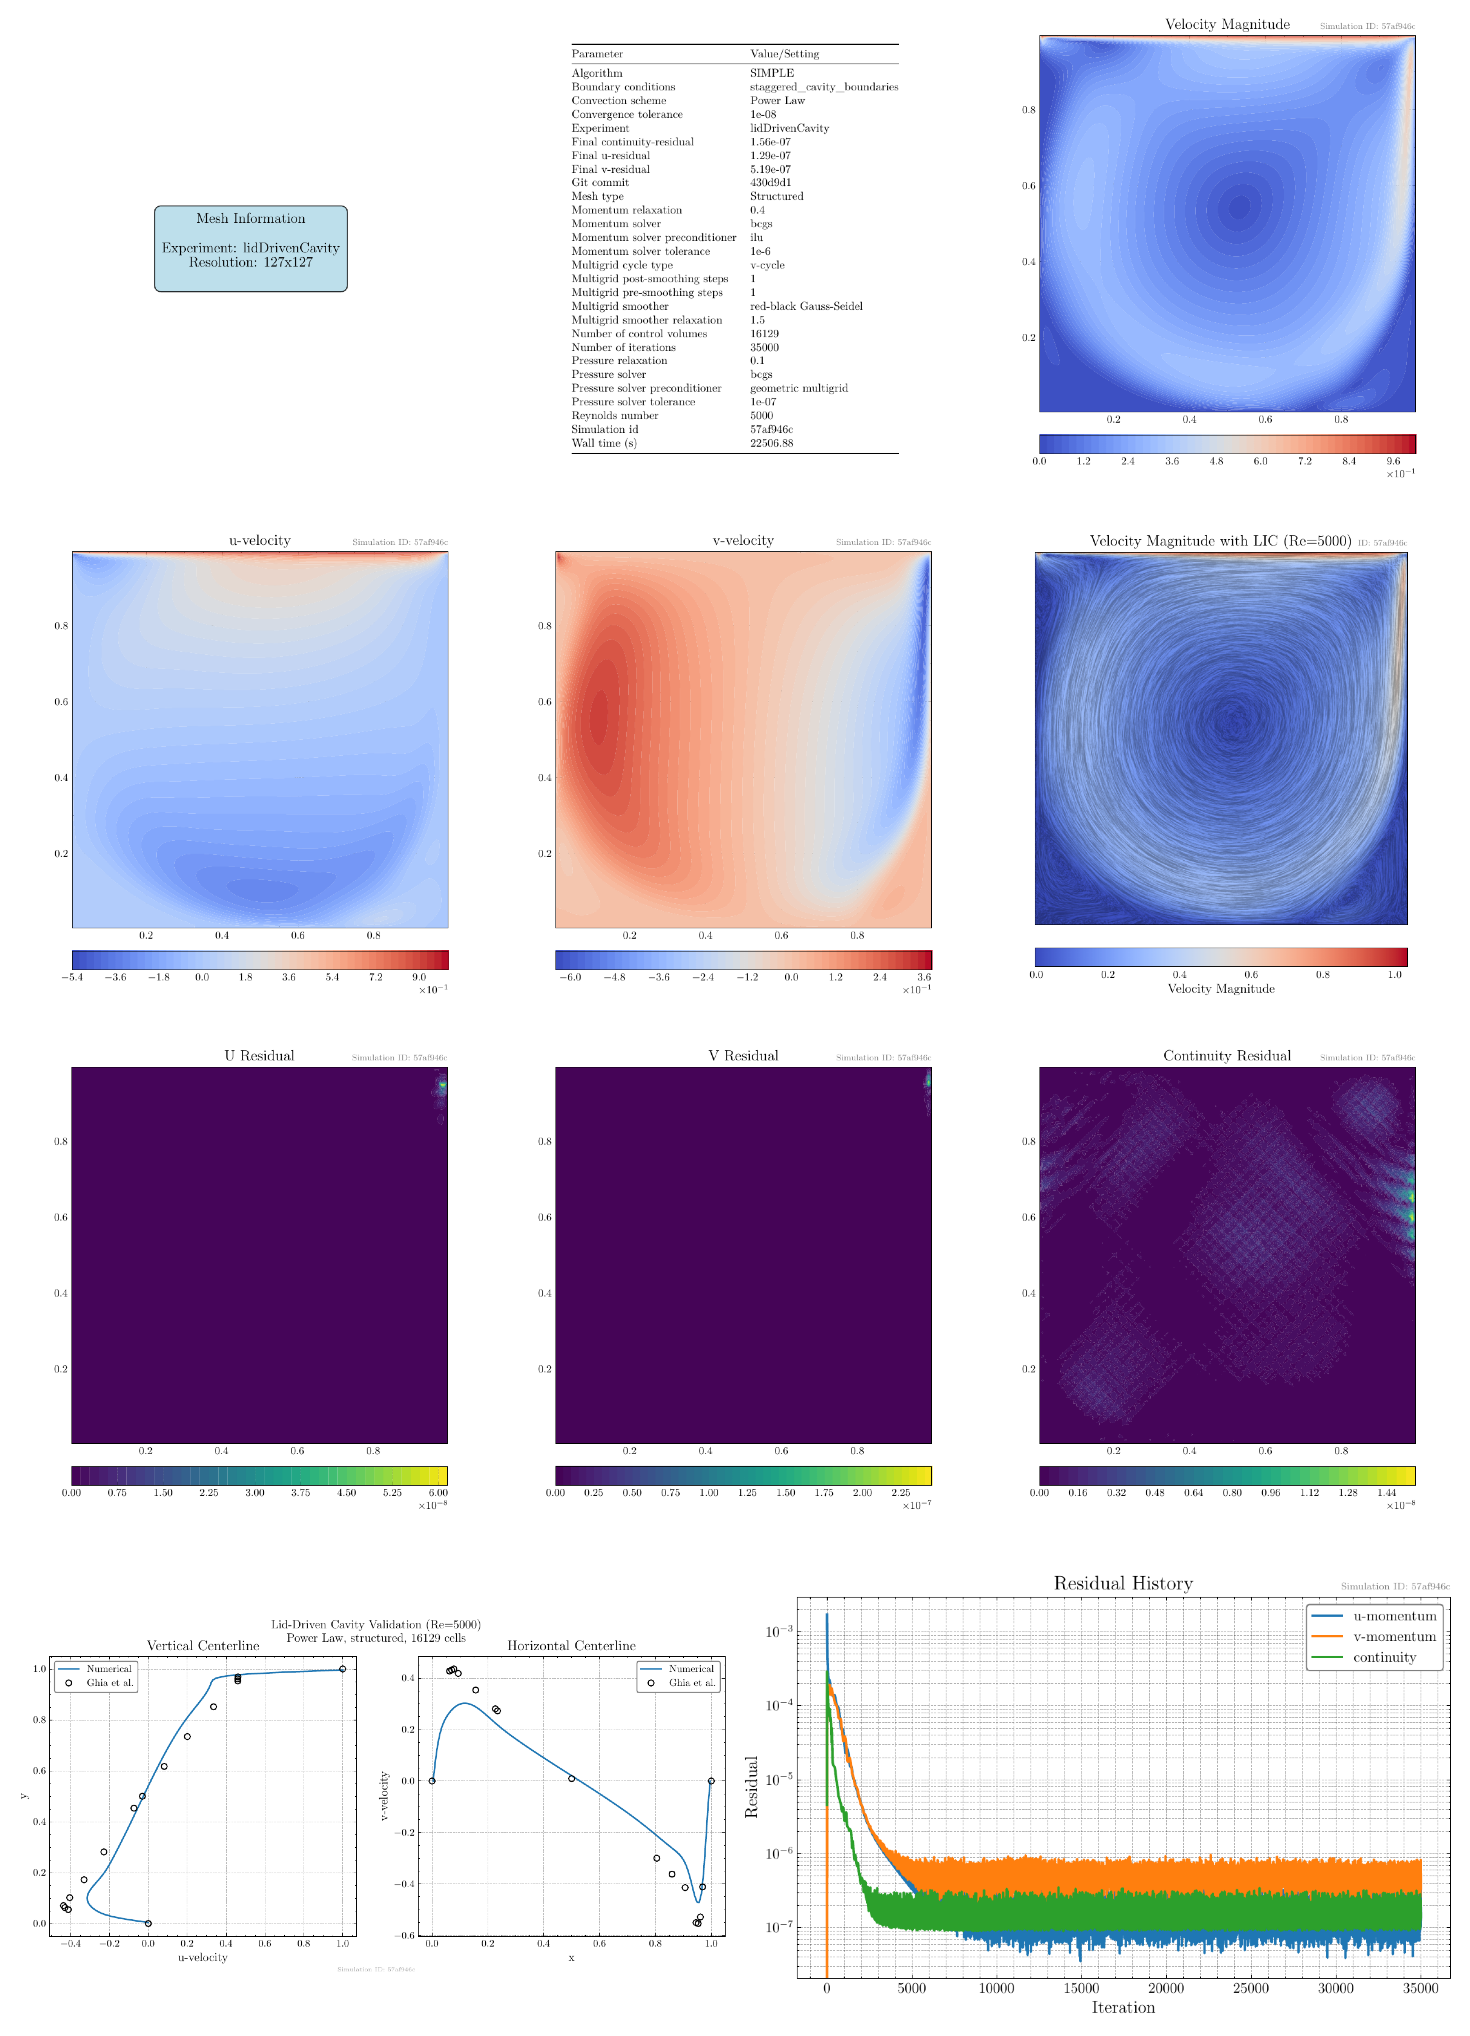
\includegraphics[width=0.85\linewidth]{AppendixPlots/lidDrivenCavity/Re_5000/127x127/lidDrivenCavity_Re5000_structured_127x127_Power Law_57af946c.pdf}
    \caption{Liddrivencavity simulation at Re=5000 using structured 127x127 (medium) mesh with Power Law discretization scheme with FMG (Simulation ID: 57af946c)}
    \label{sim.ldc.re5000.struct.med.powe}
\end{figure}
